%#!uplatex main.tex

\section{Kleinian Groups}

クライン群の学習には書籍『インドラの真珠』\cite{komori-indra201303}
(原著:~\cite{MumfordSeriesWright200204})を勧める.
インドラの真珠は数学者以外にもクライン群の魅力を伝えるために書かれた.
中には研究者レベルの高度な内容を扱う部分もあるが,高校レベルの数学と簡単なプロ
グラムを組む能力があれば,自分で図をレンダリングしながら読み進めることができる.
この章ではクライン群に関する用語を確認した後にその可視化手法と『イン
ドラの真珠』では言及のないクライン群の話題をまとめる.

\subsection{Conjugation}

クライン群を考えるうえで,我々は様々な変換を扱う.
変換に関する操作において重要となるのが\emph{共役}(\textit{Conjugation})
である.
共役を用いることで,ある変換をその性質を変えずに異なる座標において作
用させることができる.
そうすることで,複雑な変換をよりわかりやすい座標における変換としてみ
ることができる.

例えば,図\ref{fig:conju1}に示された緑色の正方形の中心における回転$\hat{T}$を
求めたいとする.
原点を中心とした回転行列はよく知られているため,これを$T$とおく.
正方形の中心までの平行移動を表わす変換を$S$とすると,$\hat{T}$
は$\hat{T} = STS^{-1}$となる.
この合成変換は次の操作と等しい.
\begin{enumerate}
 \item 図\ref{fig:conju2}のように正方形の中心を$S^{-1}$で原点へと移す.
 \item 移された正方形に回転$T$を作用させる.
 \item $S$で正方形を元の位置に戻す.これによって,$\hat{T}$で変換された正方
       形が得られる.これを図\ref{fig:conju3}に示した.
\end{enumerate}

ここで,変換$\hat{T}$を$T$の共役,$S$を共役変換とよぶ.
また,$\hat{T}$は回転と共役であるともいう.
このとき,$\hat{T}$は$T$の回転という性質を保っている.

\begin{figure}[htbp]
 \begin{minipage}{0.33\hsize}
  \center
  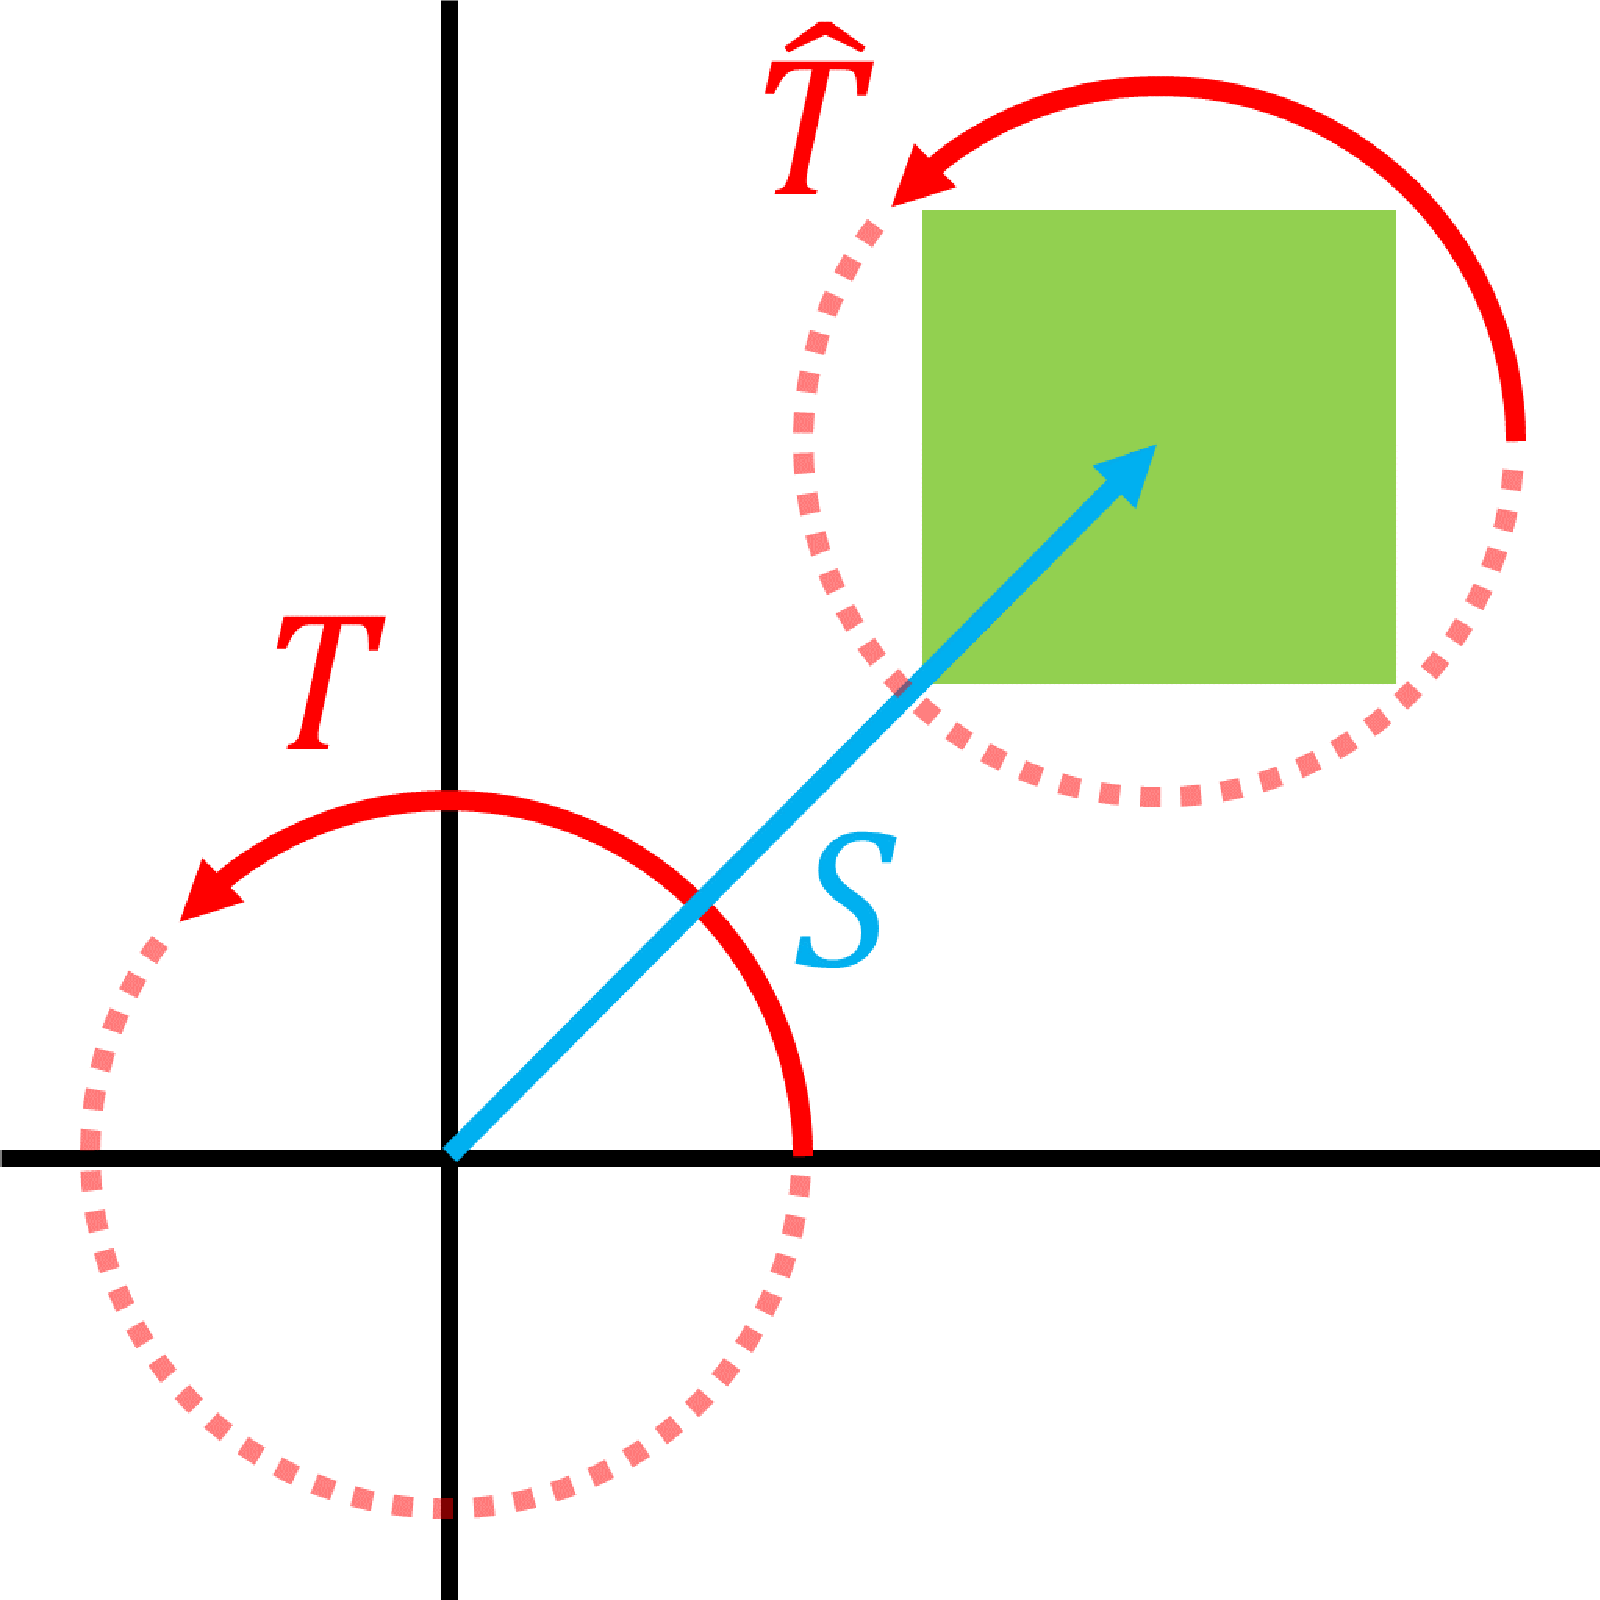
\includegraphics[width=2in, height=2in, keepaspectratio]{../img/klein/conjugation1.pdf}
   \subcaption{}
  \label{fig:conju1}
 \end{minipage}
 \begin{minipage}{0.33\hsize}
  \center
  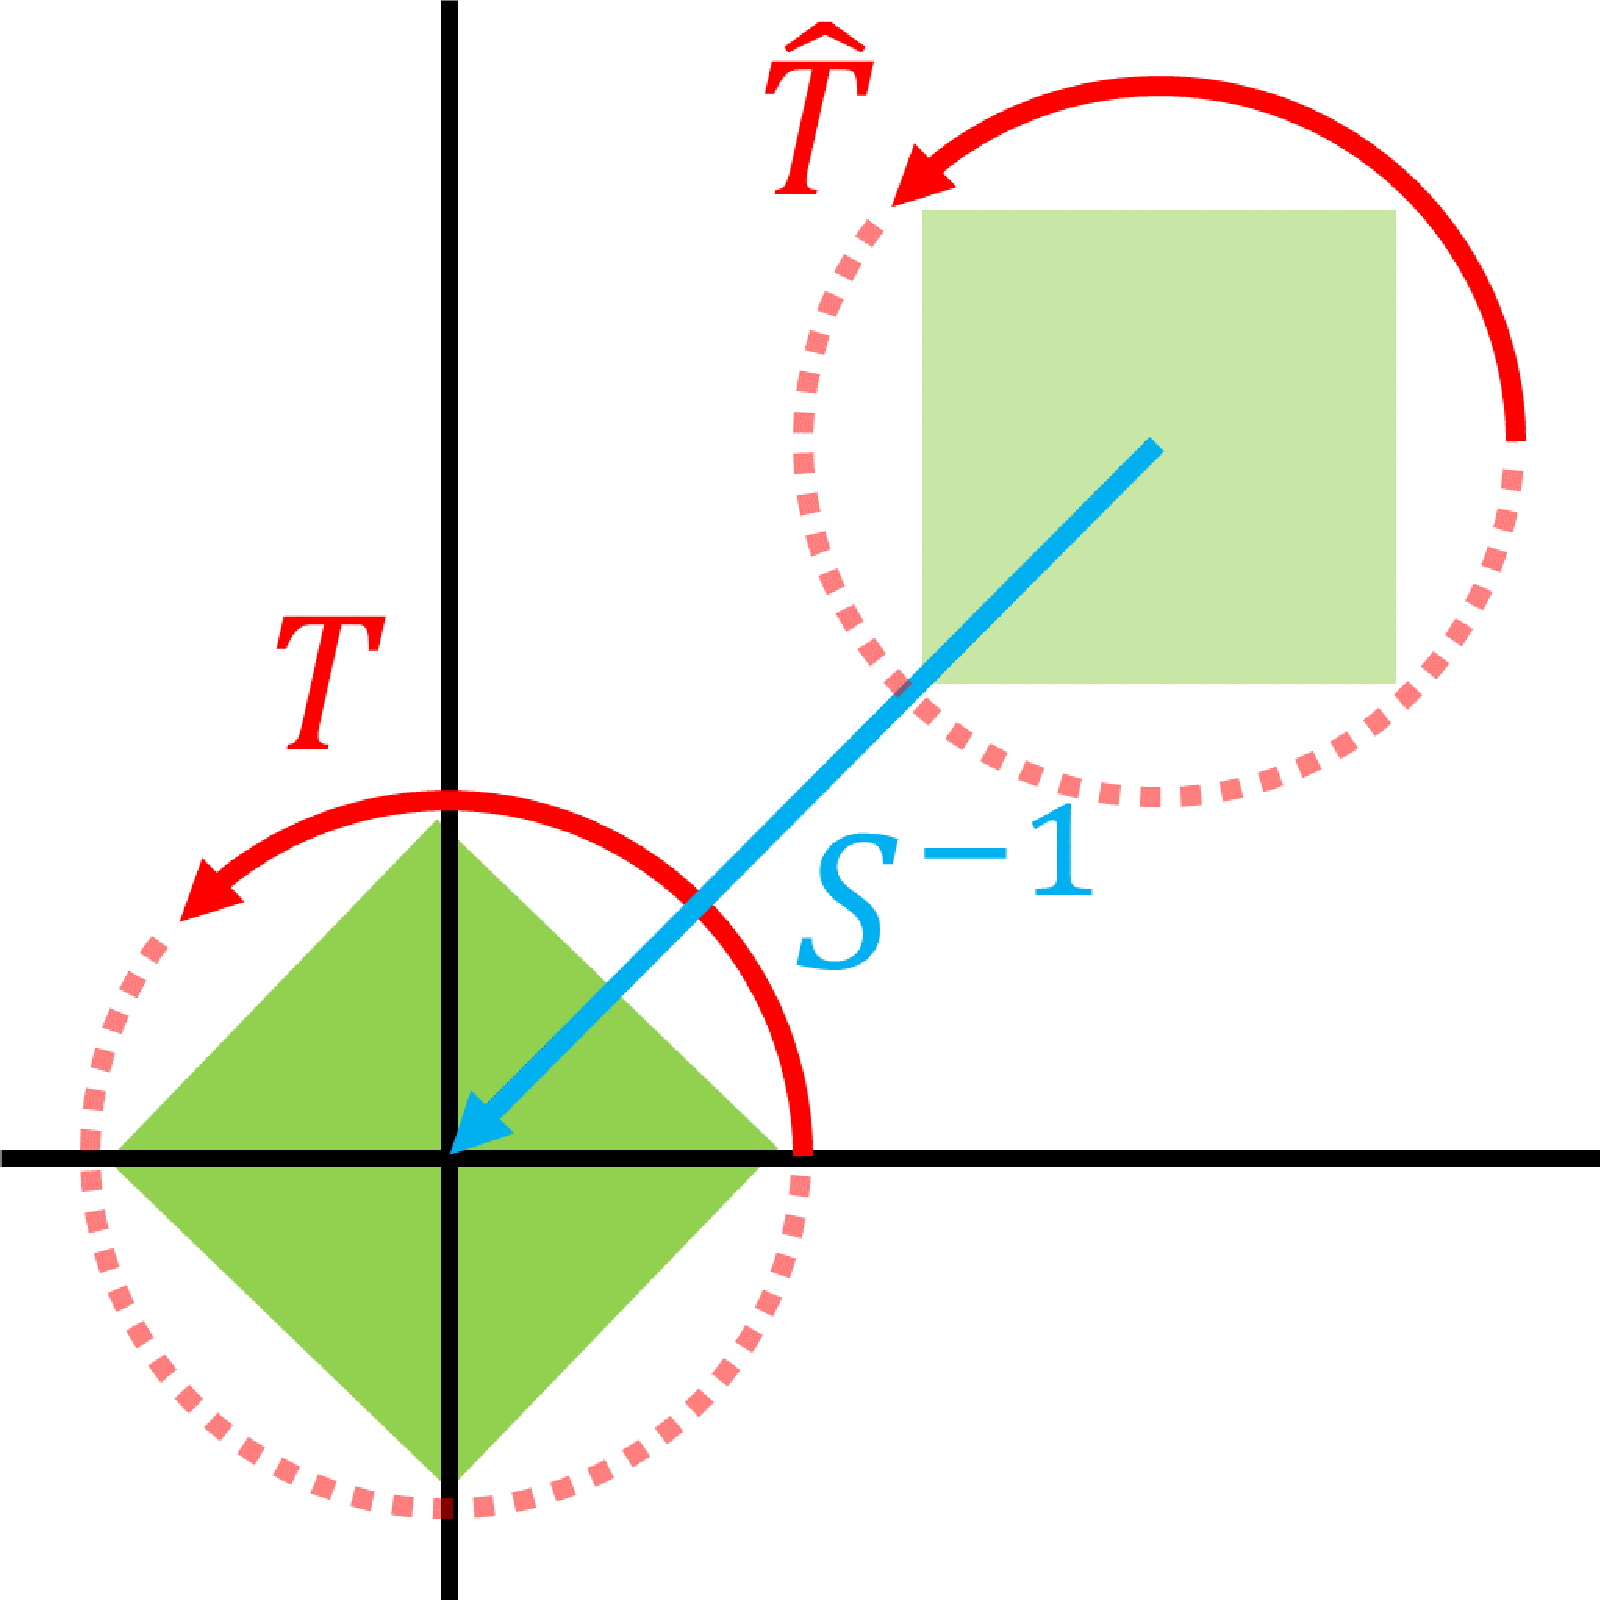
\includegraphics[width=2in, height=2in, keepaspectratio]{../img/klein/conjugation2.pdf}
  \subcaption{}
   \label{fig:conju2}
 \end{minipage}
 \begin{minipage}{0.33\hsize}
  \center
  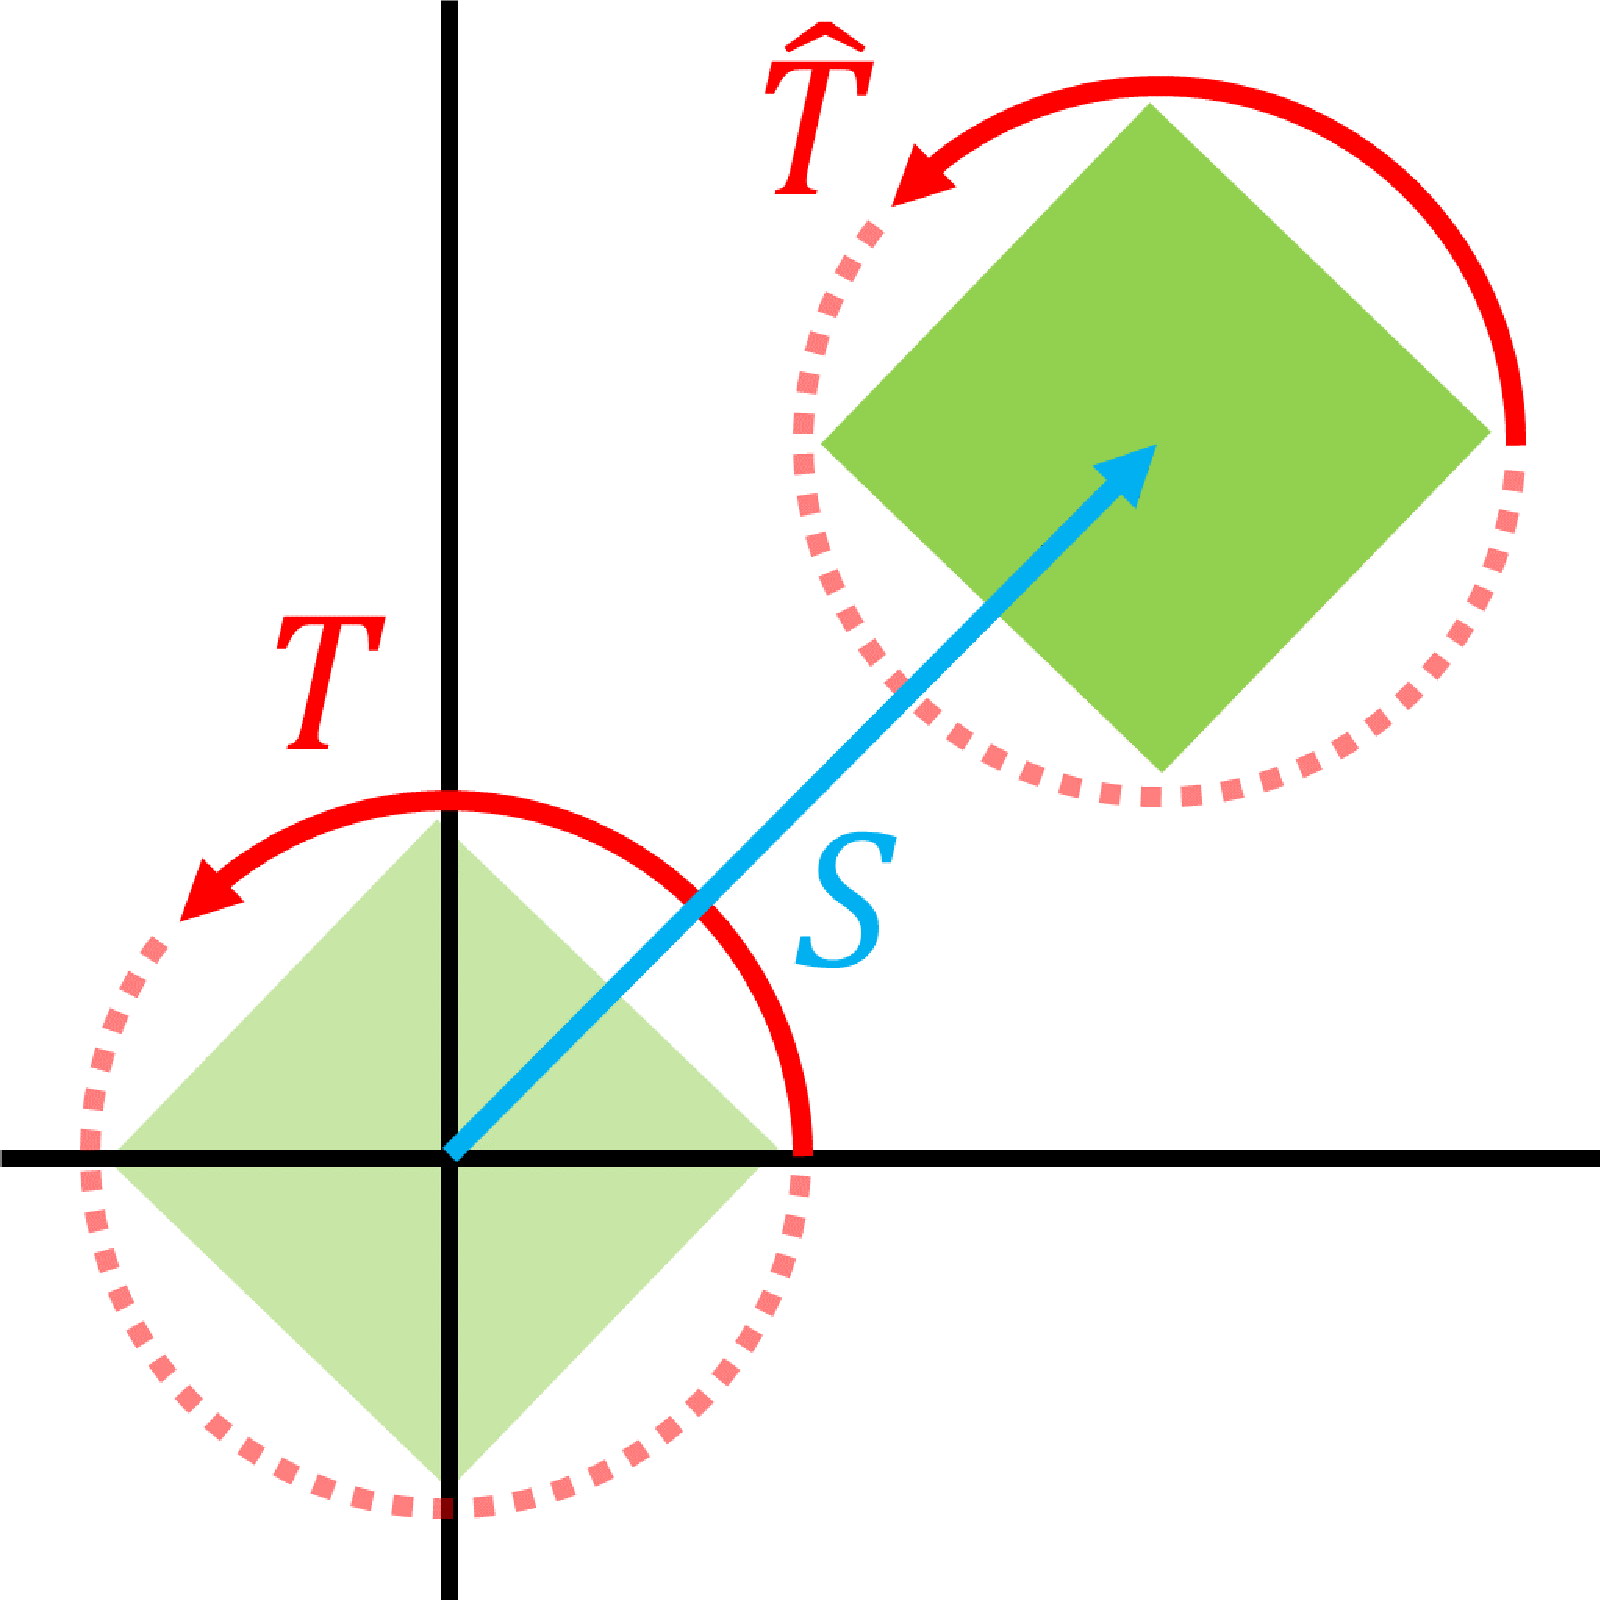
\includegraphics[width=2in, height=2in, keepaspectratio]{../img/klein/conjugation3.pdf}
  \subcaption{}
   \label{fig:conju3}
 \end{minipage}
 \caption{Conjugation}
\end{figure}

\subsection{Group}

クライン群の\emph{群}(\textit{Group})という語は変換群のことを指す.
ここでは変換の集まりだと考えるとわかりやすい.
例えば,ある変換$f(z)$,$g(z)$とそれらの逆変換という4つの変換を考える
とき,これらの変換を合成することで得られる変換の集合を群とよぶ.
また,ここで群を構成した四つの変換を\emph{生成元}(\textit{Generator})とよ
ぶ.
いま例示した群は二つの変換から生成されるので\emph{二元生成群}とよばれる
こともある.
クライン群は\emph{メビウス変換}(M\"obius Transformations)を生成元にもつ
群のなかで離散性という性質を持つものをいう.

変換の組み合わせをより扱いやすくするため,これよりそれぞれの変換を小文字
のアルファベットで表し,その逆変換を大文字で綴ることにする.
例えば,$f(z)$を$a$,$g(z)$を$b$とおくと,逆変換はそれぞれ$A$,$B$となる.
変換の合成はアルファベットを並べて書くことで表す.
例えば合成変換$f(f(g(f(p))))$は$aaba$という語で表される.
また,上付文字はその変換の無限列とする.
例えば,$\overline{a}$は$aaaaa...$というような変換$a$の無限列となる.
この無限列に対応する合成変換はどの点に作用させてもその点を変換$a$の
\emph{固定点}に移す.
変換$f(z)$の固定点とは$f(a) = a$となるような変換の前後で動くことのない点
を指す.
 \begin{align*}
  Generators =
   \begin{cases}
    a \colon f(z) \\
    A \colon f^{-1}(z) \\
    b \colon g(z) \\
    B \colon g^{-1}(z)
   \end{cases}
  \quad
  Group =
   \begin{cases}
    aab\\
    abbbaB \\
    ABBAbba \\
    baBBAbaaa \\
    ...
   \end{cases}
 \end{align*}

\subsection{M\"obius Transformations}

二次元のメビウス変換は複素平面上に,一つの無限遠点を付け加えた拡張複素
平面$\hat{\mathbb{C}}$上で定義される等角写像である.
拡張複素平面はリーマン球面とも呼ばれ,その平面全体を球面として扱うことができ
る.

メビウス変換は$a,~b,~c,~d$を$ad - bc \neq 0$を満たす任意の複素数とすると
,次のように表される.
\begin{align*}
 f(z) = \frac{az + b}{cz + d}
\end{align*}
メビウス変換はその形から,一次分数変換ともよばれる.
我々になじみの深い平行移動,拡縮や回転といった変換もメビウス変換に含まれる.

メビウス変換は以下のように係数を2×2の複素数行列として扱うことで,
代数として操作することができる.
例えば,次のように合成変換を行列の積として表すことができる.
\begin{align*}
  m = \left(
 \begin{array}{ccc}
  a & b \\
  c & d
 \end{array}
 \right),~
 n = \left(
 \begin{array}{ccc}
  e & f \\
  g & h
 \end{array}
 \right),~
 mn = \left(
 \begin{array}{ccc}
  a & b \\
  c & d
 \end{array}
 \right)
\left(
 \begin{array}{ccc}
  e & f \\
  g & h
 \end{array}
 \right)
\end{align*}

メビウス変換はおおまかに\emph{放物型}(\textit{Parabolic}),\emph{斜航
型}(\textit{Loxodromic}),\emph{楕円型}(\textit{Elliptic})の三種類に分
類される.
斜航型変換と楕円型変換は二つの固定点をもち,放物型変換は一つの固定点をもつ.
斜航型変換は単純な回転を除いた複素数による拡縮と共役である.
また斜航型変換の中でも正の実数による拡縮と共役である
変換を\emph{双曲型}(\textit{Hyperbolic})変換とよぶ場合もある.
放物型変換は平行移動と共役で,楕円型変換は回転と共役である.

クライン群の描画において,メビウス変換の分類は重要である.
なぜならば,楕円型変換を含む群の多くはクライン群にはなりえない.
また,放物型変換は固定点への収束が遅いという特徴をもつ.
これは後述する極限集合の描画の際に考慮することになる.

\subsection{Circle Inversion}

円は複素平面に作用するメビウス変換を考えるうえで重要な図形である.
メビウス変換は円円対応という性質をもち,任意の円を円に移す.
ここでは\emph{円に関する反転}(\textit{Circle Inversion})という操作をみる.
これは円弧を軸とみた鏡映変換であり,円の中心と無限遠点が入れ替えられる.

点aを中心とする半径rの円に関する反転を$I(z)$とすると,式は次のようになる.
\begin{align*}
I(z) =
 \begin{cases}
  \frac{r^2}{\overline{z - a}} + a \quad & z \in \mathbb{C} - \{a\} \\
  a \quad & z = \infty\\
  \infty \quad & z = a
 \end{cases}
\end{align*}
また,半径が無限大の円は直線と考えることができるので,その円に関する反転
は直線に関する反転と考えることができる.

図\ref{fig:circleInversion}は中央の黒の円弧をもつ円に関する反転によって
移される図形を可視化したものである.
緑色の矩形を観察すると,変換の前後で大きく形を歪められているが,その角は直
角が保たれている.
直線は無限遠点が円の中心へと移るため,反転円の中心を通る円となる.
また,赤の円は操作の前後で形が保たれている.

円に関する反転は複素平面の向き付けを逆にしてしまうため,メビウス変換では
ない.
しかし,二つの円の反転の組が双曲型のメビウス変換となる.
さらに,偶数個の円の反転を組み合わせることでその他の種類のメビウス
変換を構成することができる.
円に関する反転はメビウス変換を構成する変換の最小単位ともいえる.

また,円を球に拡張することで球に関する反転を考えることができる.
これを用いて三次元空間に作用するメビウス変換を構成することもできる.

\begin{figure}[htbp]
 \center
 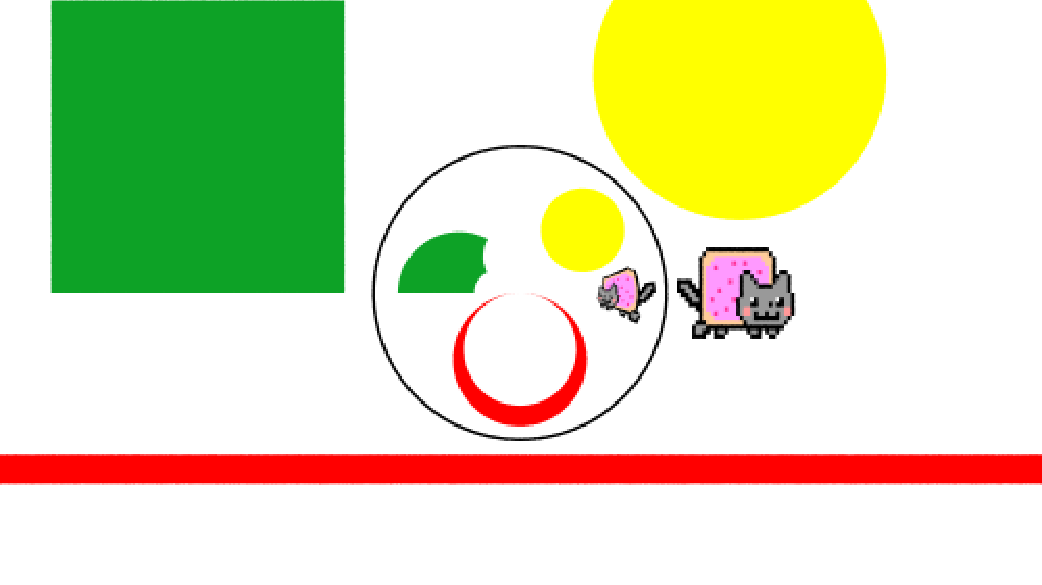
\includegraphics[width=3in, height=3in, keepaspectratio]{../img/klein/circleInversion.pdf}
 \caption{Circle inversion}
 \label{fig:circleInversion}
\end{figure}

\subsection{Stereographic Projection}

球面上の点を拡張複素平面へと写像するためには,\emph{立体射影}({\it
stereographic projection})とよばれる方法がよく使われる.
地図の制作のため,地球のような球面を平面に投影する方法が様々に考えられて
きたが,それらの手法の中でも立体射影は角度と円を保つため,メビウス変換と相性が良い.
複素平面を球面でみることによって,メビウス変換の作用全体をよくみることが
できる.
図\ref{fig:stereoProject}に立体射影を図示した.赤の円は単位円,
青の直線はX軸を表している.

立体射影の操作は非常に簡単である.球の断面による模式図を図
\ref{fig:stereoProjectSlice}に示した.
緑の円が球の断面を表し,黒の直線が平面の断面を表している.
球の北極を$N$,球面上の点を$P$,$P$を立体射影で移した複素平面上の点を
$P'$とおく.
$P'$は$N$から$P$へと引いた直線と平面との交点となる.

直径1の球面を南極が$(0,~0,~0)$に,北極が$(0,~0,~1)$になるようにおき,複
素平面を複素数$x + yi$が$(x,~y,~0)$となるようにおく.
球面上の任意の点を$(u,~v,~w)$とし,立体射影によって移る点を$(x,~y,~0)$と
すると,立体射影の公式は次のようになる.
\begin{align*}
 x = \frac{u}{1 - w},~y = \frac{v}{1 - w}
\end{align*}
また,立体射影の逆は次のようになる.
\begin{align*}
 u = \frac{x}{x^2 + y^2 + 1},~v = \frac{y}{x^2 + y^2 + 1},~
 w = \frac{x^2 + y^2}{x^2 + y^2 + 1}
\end{align*}

\begin{figure}[htbp]
 \begin{minipage}{0.5\hsize}
  \center
  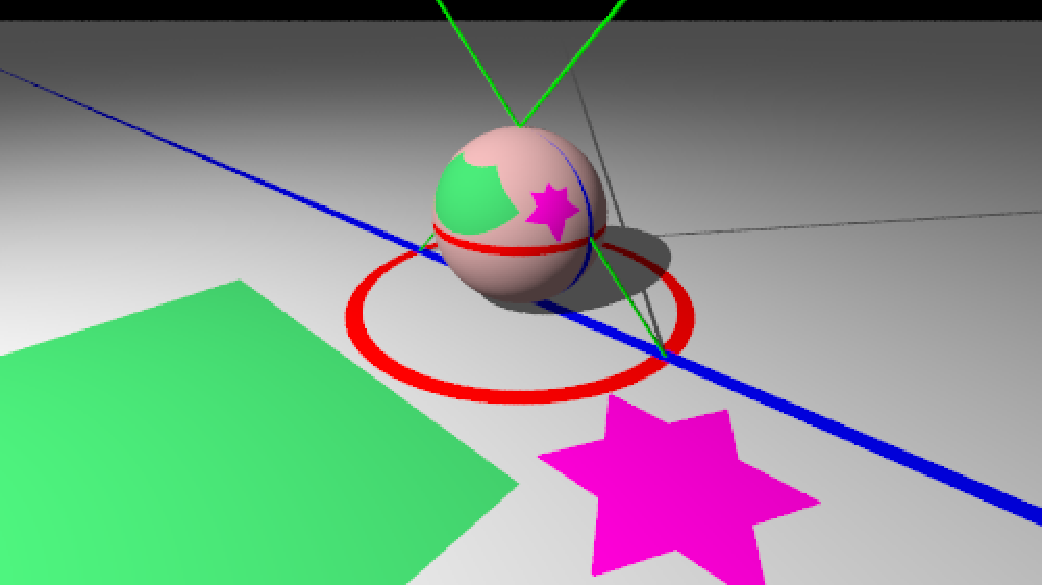
\includegraphics[width=3in, height=3in, keepaspectratio]{../img/klein/stereoProject.pdf}
  \caption{Stereographic Projection}
  \label{fig:stereoProject}  
 \end{minipage}
 \begin{minipage}{0.5\hsize}
  \center
  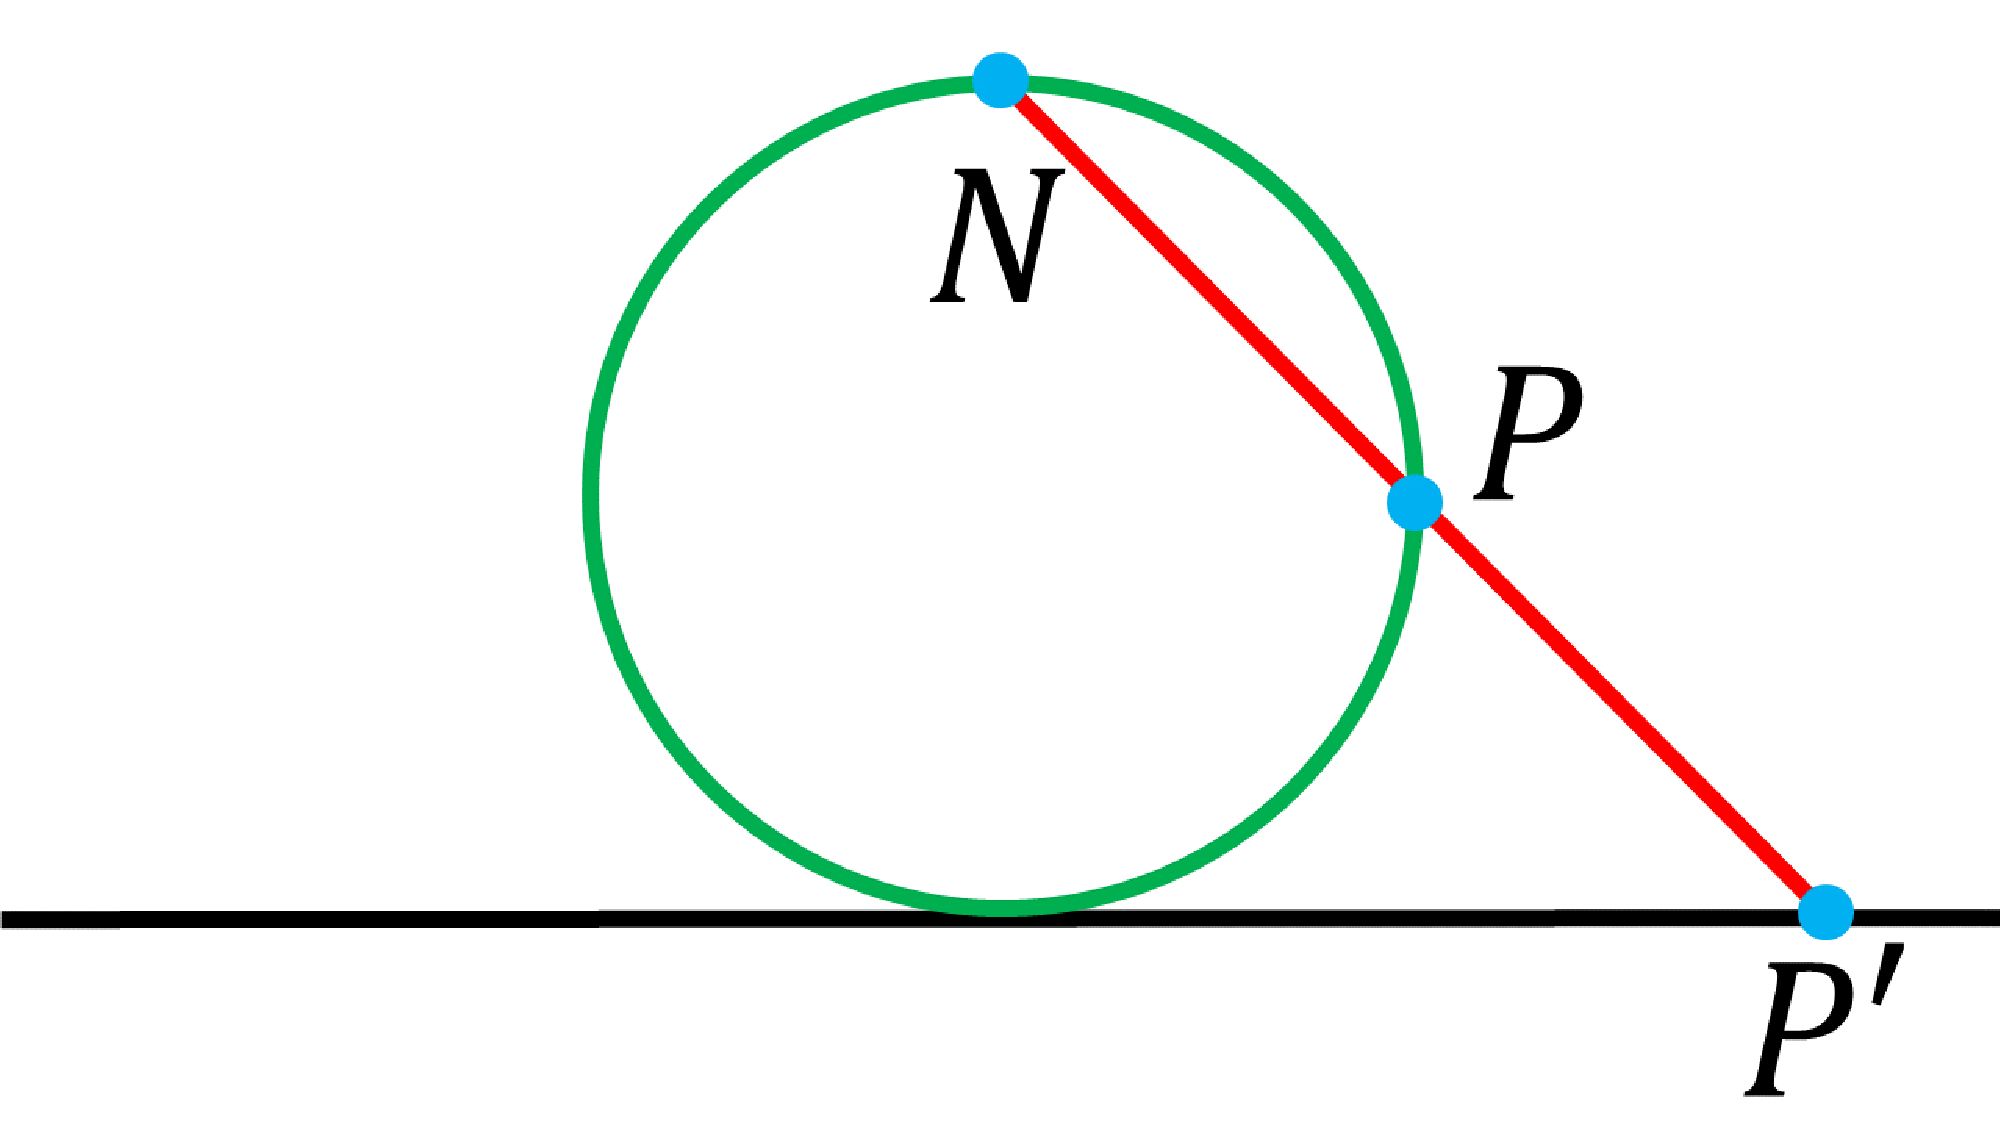
\includegraphics[width=3in, height=3in, keepaspectratio]{../img/klein/stereoProjectSlice.pdf}
  \caption{slice}
  \label{fig:stereoProjectSlice}
 \end{minipage}
\end{figure}

Saul Schleimer,Henry Segermanはメビウス変換を利用して全天球画像(上下左
右360度パノラマ写真)を編集することを考案した\cite{bridges2016-15}.
彼らは\emph{ドロステ効果}(\textit{Droste-effect})をもつ再
帰的な画像をメビウス変換を用いてつくる手法を提案している
\footnote{Spherical Droste video:
\url{https://www.youtube.com/watch?v=qvh-EAipIUk}}.

全天球画像はその名の通り球面に張り付けられた画像であるので,メビウス変
換で角度を保ったまま編集を加えることができる.
また,全天球画像は正距円筒図法(Equirectangular map)で扱われることも多い.
この図法は縦軸に緯度,横軸に経度をとり,球面をそのまま写像するものである.
メビウス変換で球面の画像を変形したものを正距円筒図法で写像すると興味深い
効果をみることができる.

図\ref{fig:sphericalRotation},\ref{fig:sphericalTranslation},
\ref{fig:sphericalScaling}は図\ref{fig:sphericalStandard}の格子模様
に対して簡単なメビウス変換を作用させたものである.
複素平面,リーマン球面,その正距円筒図,そして全天球画像の一部を注視した
図を示した.

\begin{figure}[htbp]
 \begin{minipage}{0.5\hsize}
  \center
  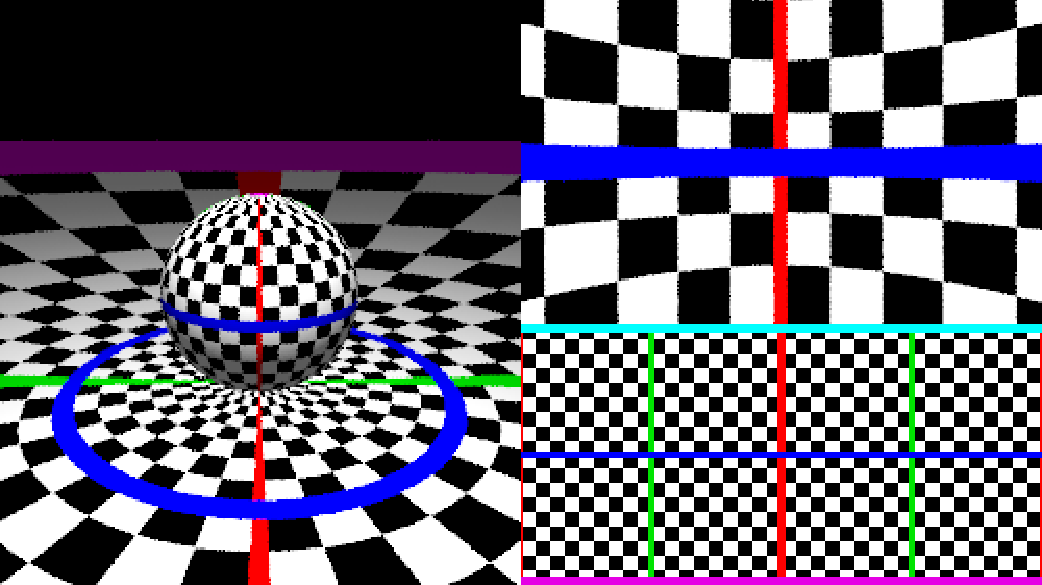
\includegraphics[width=3in, height=3in, keepaspectratio]{../img/klein/spherical.pdf}
  \subcaption{Standard}
  \label{fig:sphericalStandard}
 \end{minipage}
 \begin{minipage}{0.5\hsize}
  \center
  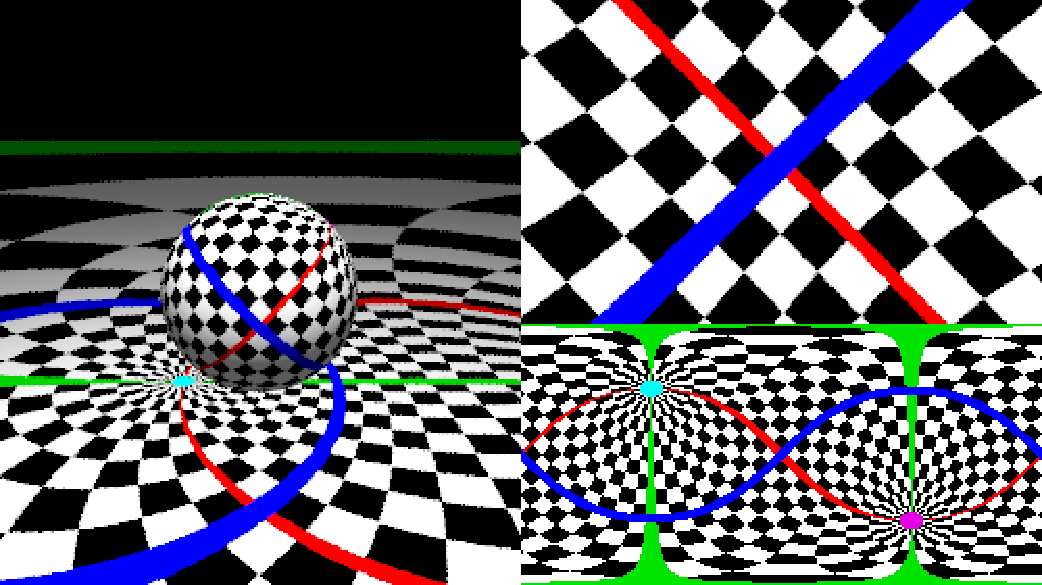
\includegraphics[width=3in, height=3in, keepaspectratio]{../img/klein/sphericalRotation.pdf}
  \subcaption{Rotation}
  \label{fig:sphericalRotation}
 \end{minipage}
 \begin{minipage}{0.5\hsize}
  \center
  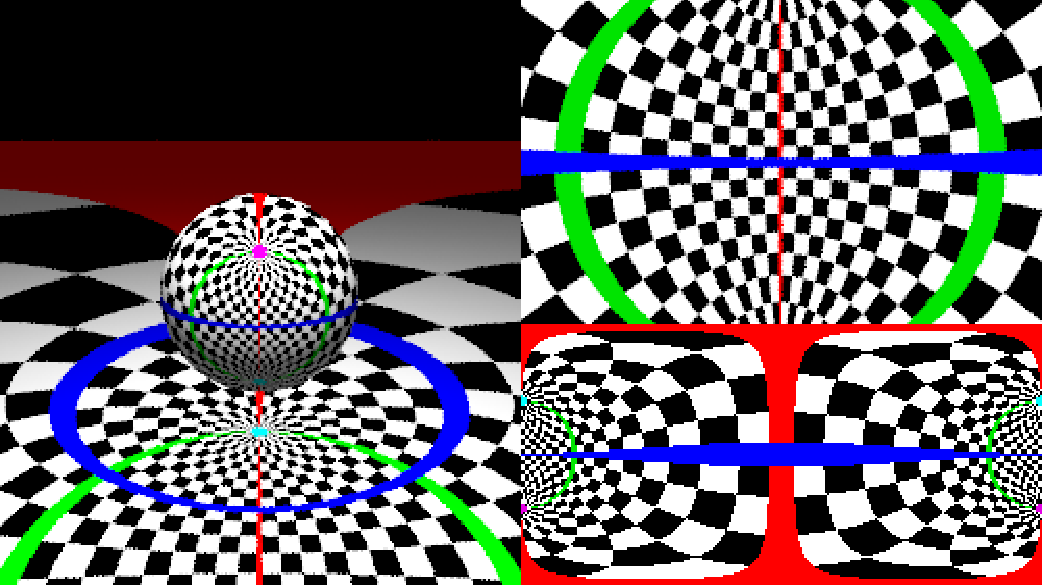
\includegraphics[width=3in, height=3in, keepaspectratio]{../img/klein/sphericalTranslation.pdf}
  \subcaption{Translation}
  \label{fig:sphericalTranslation}
 \end{minipage}
 \begin{minipage}{0.5\hsize}
  \center
  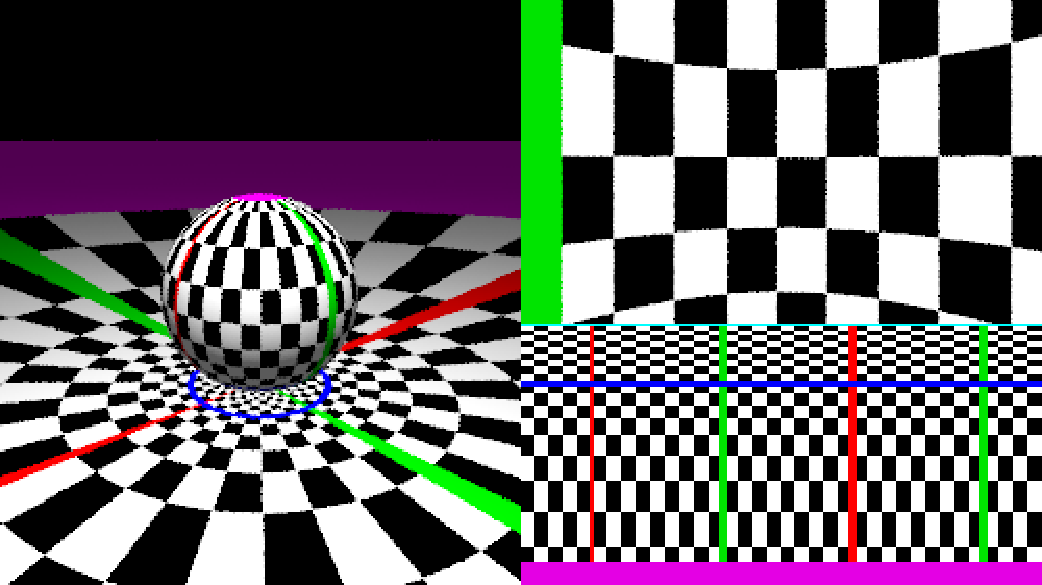
\includegraphics[width=3in, height=3in, keepaspectratio]{../img/klein/sphericalScaling.pdf}
  \subcaption{Scaling}
  \label{fig:sphericalScaling}
 \end{minipage}
 \caption{Spherical images}
 \label{fig:spherical}
\end{figure}

\subsection{Visualization with Graph Traversal Approach}

群を構成する合成変換の全組み合わせは変換の語で構成される有向グラフで表現
することができる.
図\ref{fig:wordTree}にそのようなグラフの例を示した.
この図では変換$a$,$b$とそれらの逆変換である4種類の変換の合成の組合せを表
わしている.
例えば,$a$というラベルがふられたノードには外側へ3本のエッジが
張られ$ab,~aa,~aB$という合成変換を表すノードへとつながっている.
また,$aA$は逆変換を合成することになるので,このグラフ上では逆戻りを表し
ている.
このようなグラフは\emph{ケーリーグラフ}(\textit{Cayley graph})とよばれる.
このグラフを探索することで群の構成要素である合成変換を列挙していくことが
できる.この節ではケーリーグラフを探索することで得られる合成変換を用いて
群の作用を可視化する方法をみる.

群を構成するためには複数のメビウス変換が必要である.しかし,メビウス変換
は四つの複素数で構成されているため自由度が高く,そのまま群を考えることは
難しい.
そのため,群の生成元を得るための「レシピ」が用いられる.
例えば,『インドラの真珠』では「おばあちゃんのレシピ」とよばれるレシピが
紹介されている.
このレシピは二つの複素数$t_a$,$t_b$をパラメータにとり,以下のような操作
で二つの生成元を得ることができる.
\begin{enumerate}
 \item 二つの複素数$t_a$,$t_b$を選ぶ.
 \item  二次方程式
        $x^2 - t_a t_b x + t_a^2 + t_b^2 = 0 \text{の一方の解}x\text{を
        選び},~t_{ab}= x \text{とする. }$
 \item 複素数$z_0$を次のように定義する.
       \begin{align*}
        z_0 = \frac{(t_{ab} -2)t_b}{t_b t_{ab} - 2 t_a + 2it_{ab}}
       \end{align*}
 \item 生成元の行列は次のようになる.
        \begin{align*}
       &a = \left(
      \begin{array}{ccc}
       \frac{t_a}{2} & \frac{t_a t_{ab} - 2 t_b + 4i}{(2 t_{ab} + 4)z_0} \\
       \frac{(t_a t_{ab} - 2 t_b -4i)z_0}{2 t_{ab} - 4} & \frac{t_a}{2}
      \end{array}
     \right)\\
 &b = \left(
      \begin{array}{ccc}
       \frac{t_b - 2i}{2} & \frac{t_b}{2} \\
       \frac{t_b}{2} & \frac{t_b + 2i}{2}
      \end{array}
     \right)
        \end{align*}
\end{enumerate}
このように,八つの複素数のパラメータをもつ二元生成群を二つの複素数から生
成することができるため,扱いやすくなる.
また,「おばあちゃんのレシピ」は群を可視化した際に綺麗な図がレンダリング
されるように共役によって調整されている.

\begin{figure}[htbp]
 \center
 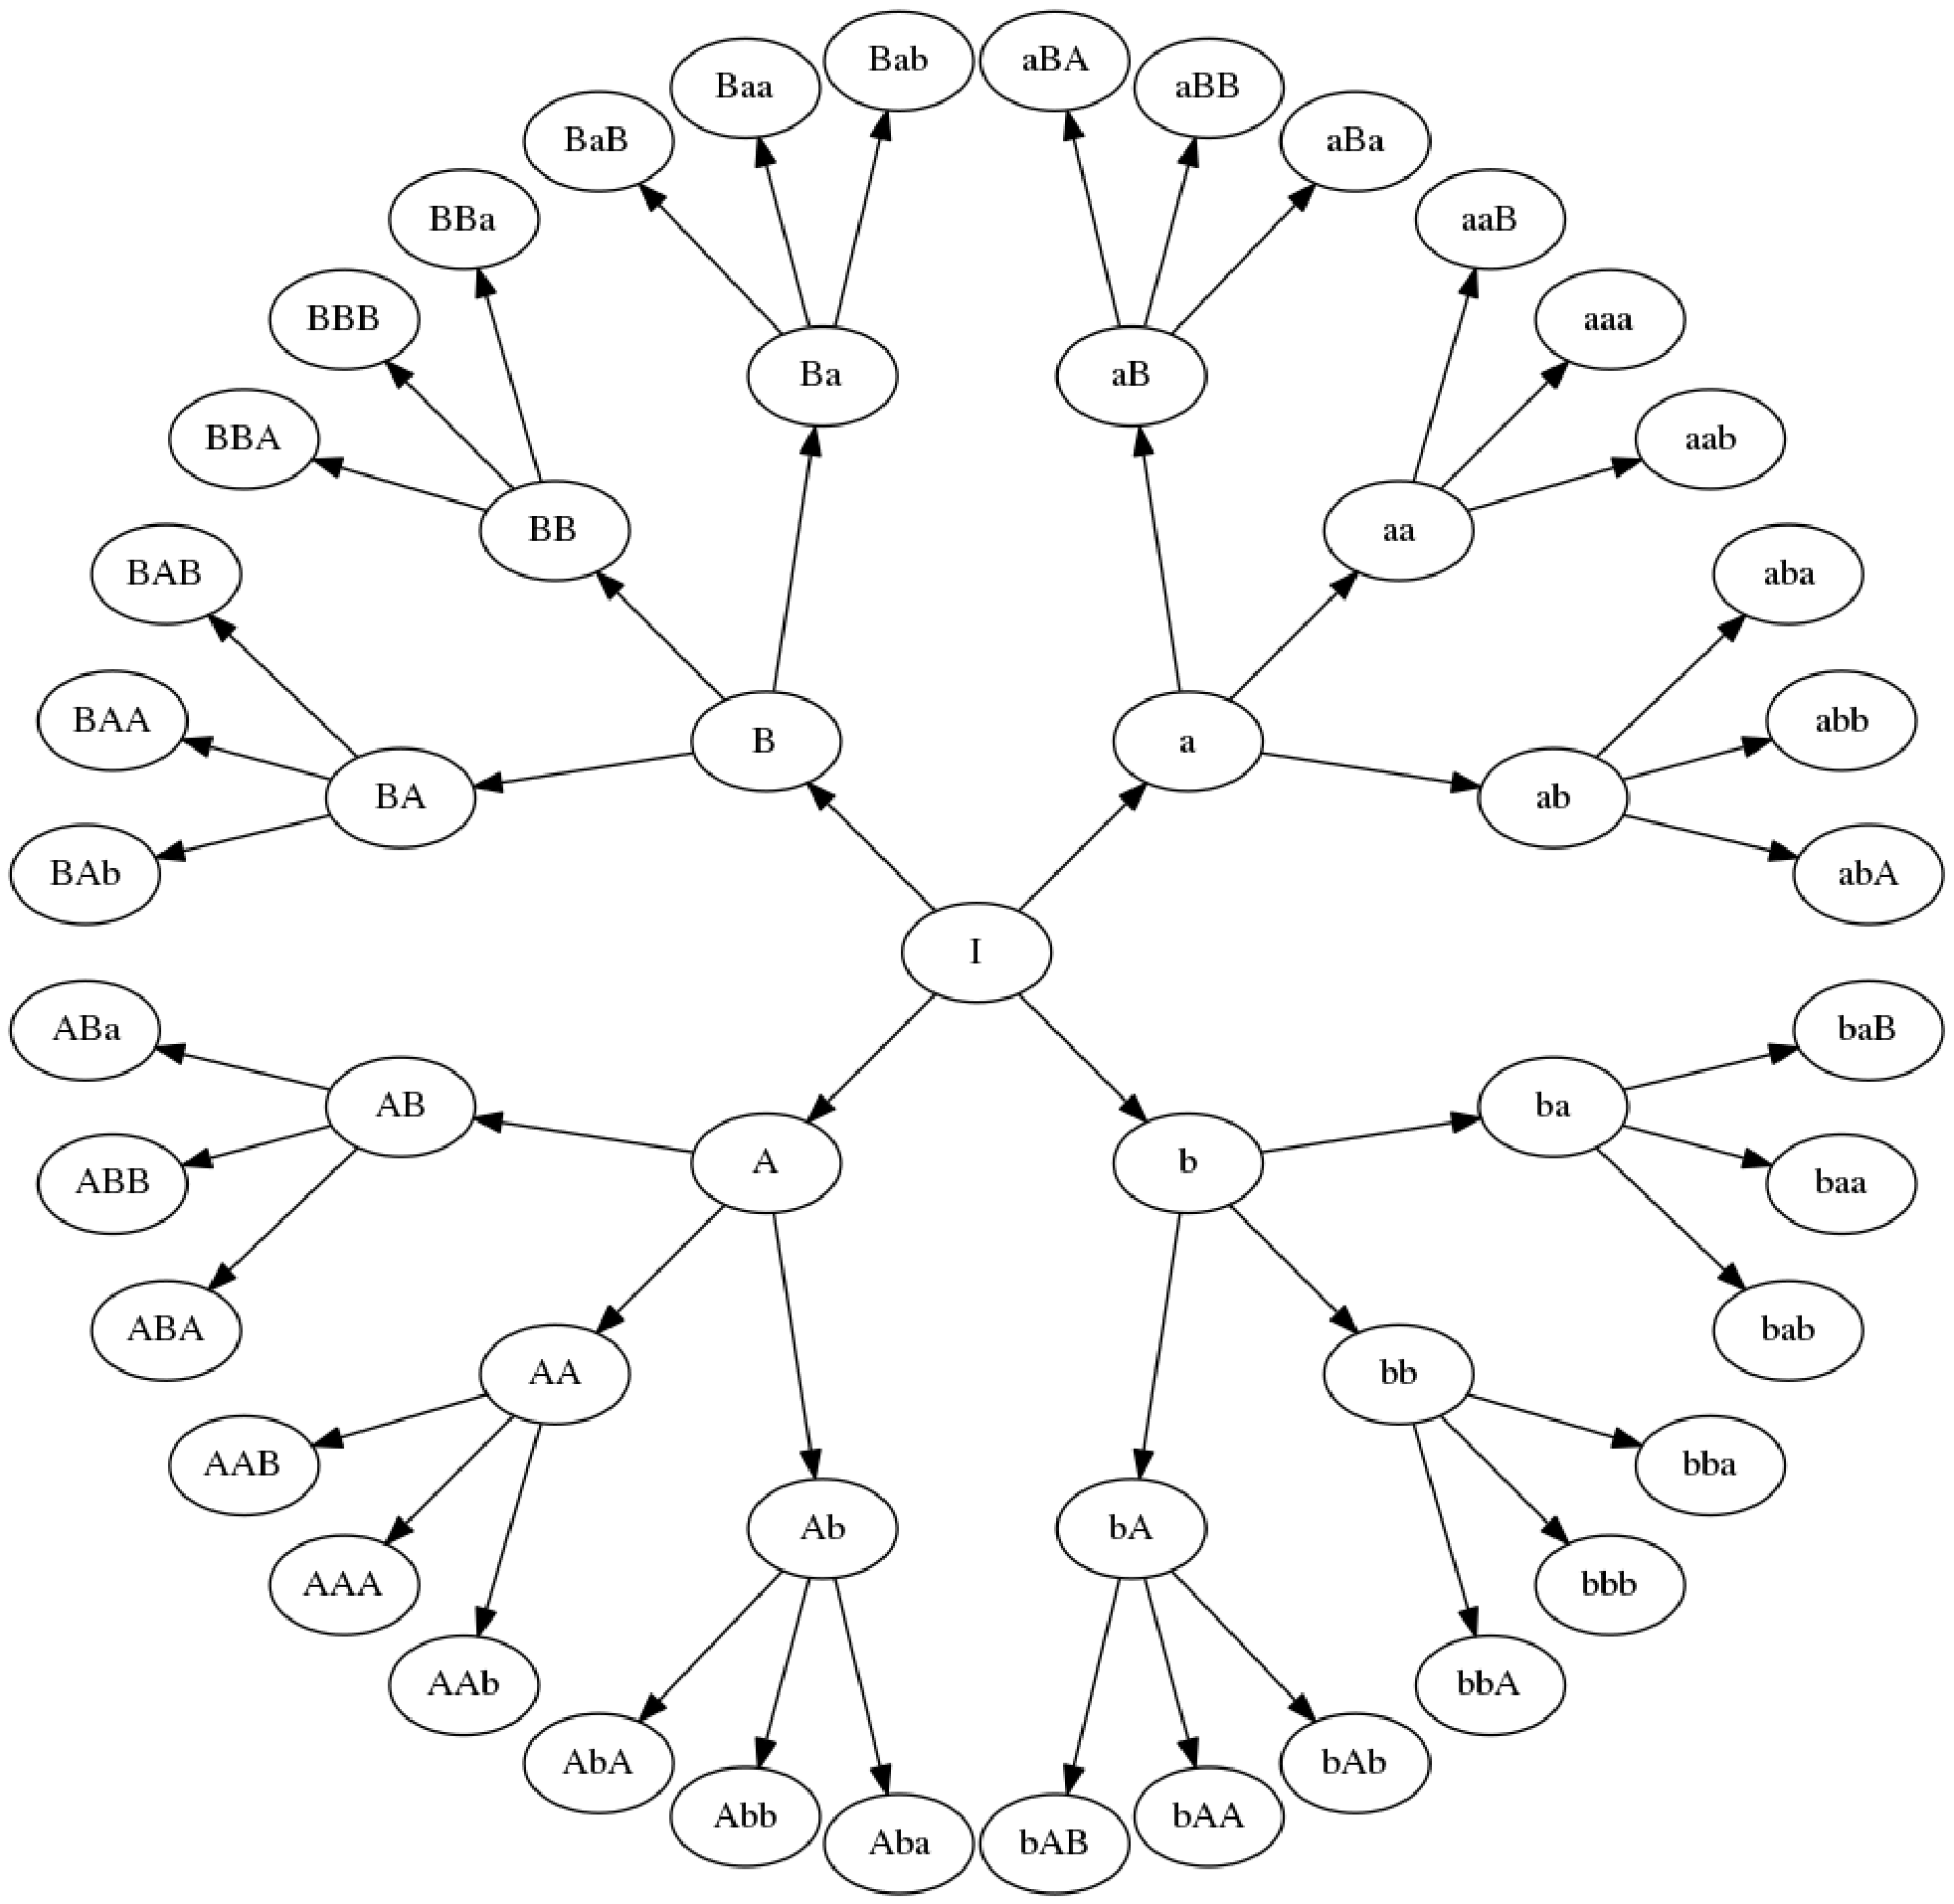
\includegraphics[width=3in, height=3in, keepaspectratio]{../img/klein/wordTree.pdf}
 \caption{Word Tree}
 \label{fig:wordTree}
\end{figure}

\subsubsection{The Orbit of Transformations}

群を可視化する方法の一つは群の軌道を描画するというものである.
図\ref{fig:schottky}に円の反転で構成される群の軌道を描いた.
四つの大きな円の内側にたくさんの円が入れ子状に描かれている.
これが円の軌道である.また,円列の極限を\emph{極限集合}(\textit{Limit set})と
よぶ.
円の反転は変換自体を円という図形で表現できるため,その作用を理解しやすい.
四つの円はそれぞれに円の反転の組み合わせが作用させられることにより,その内側へと移され
ていく.

図\ref{fig:orbit}には中央に描かれた六芒星の軌道を描いた.
これも六芒星が周囲の円による反転の組み合わせで移されている.
この軌道も極限集合へと収束していく.
\begin{figure}[htbp]
 \begin{minipage}{0.49\hsize}
  \center
  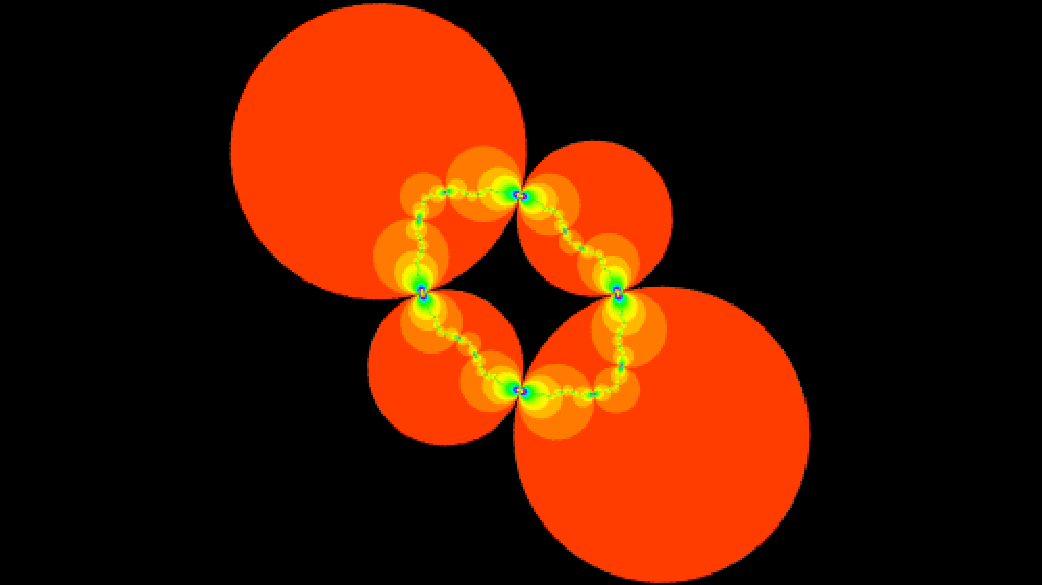
\includegraphics[width=3in, height=3in, keepaspectratio]{../img/klein/schottkyCircles.pdf}
  \caption{The orbit of circles}
  \label{fig:schottky}
 \end{minipage}
 \begin{minipage}{0.49\hsize}
  \center
  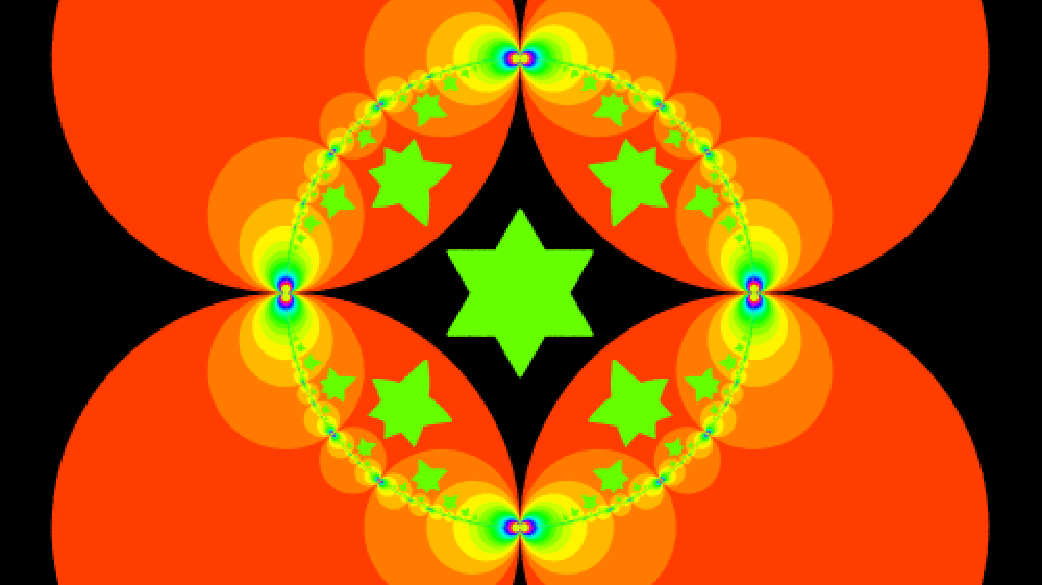
\includegraphics[width=3in, height=3in, keepaspectratio]{../img/klein/starOrbit.pdf}
  \caption{The orbit of hexagram}
  \label{fig:orbit}
 \end{minipage}
\end{figure}

図\ref{fig:schottky}のような円の軌道を計算する過程は以下のようになる.
\begin{enumerate}
 \item 図\ref{fig:level0}に示した四つの大きな円を反転円とよぶ.
       これらの円に関する反転を生成元とする群の軌道を描くことを考える.
 \item それぞれの反転円に関する反転は図\ref{fig:level0inv}のように,自分以外の反
       転円を自身の内側に移す.
 \item この操作を四つの反転円でおこなうと,それぞれの円の内側には三つの円が移
       され,図\ref{fig:level1}のように合せて12個の小円ができる.
 \item 次に,新たにできた小円に対してもその小円が属している反転円以外の反転を作
       用させる.図\ref{fig:level1inv}では,白く縁取りされた円に関する
       反転でその他の小円が移される様子を描いた.
 \item この操作も四つの反転円で行なうと,図\ref{fig:level2}のように小円の
       下に新たな小円ができる.
 \item このことを繰り返すと,最終的に図\ref{fig:levelMax}を得ることができる.
\end{enumerate}

\begin{figure}[htbp]
 \begin{minipage}{0.33\hsize}
  \center
  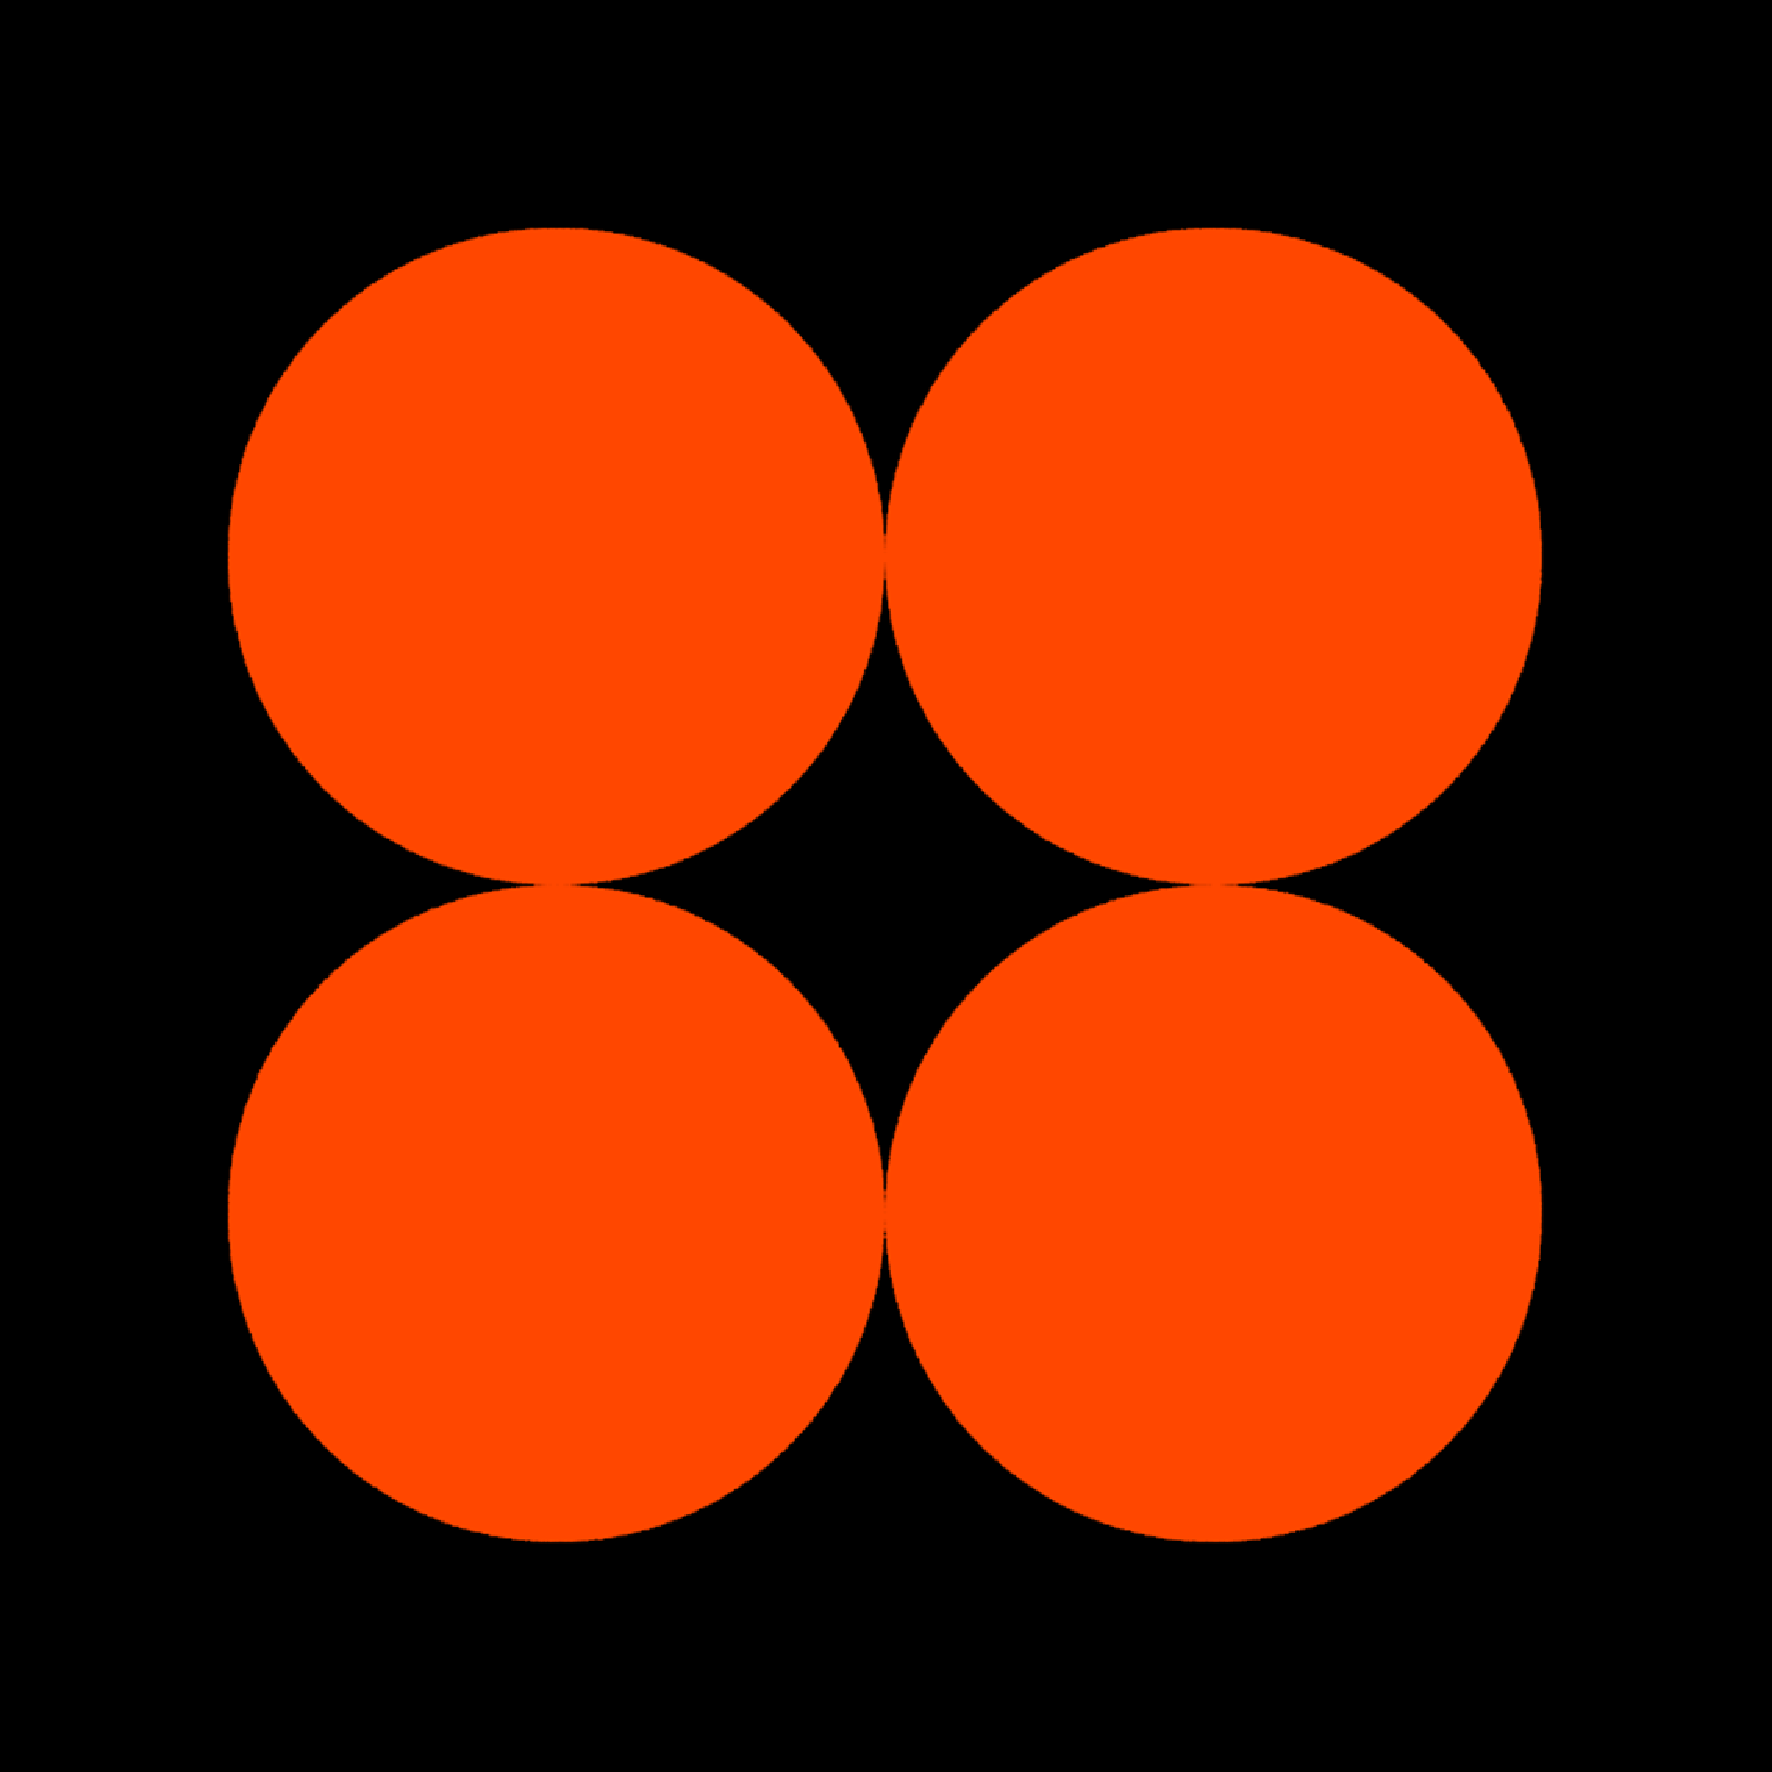
\includegraphics[width=2in, height=2in, keepaspectratio]{../img/klein/orbit/level0.pdf}
   \subcaption{}
  \label{fig:level0}
 \end{minipage}
 \begin{minipage}{0.33\hsize}
  \center
  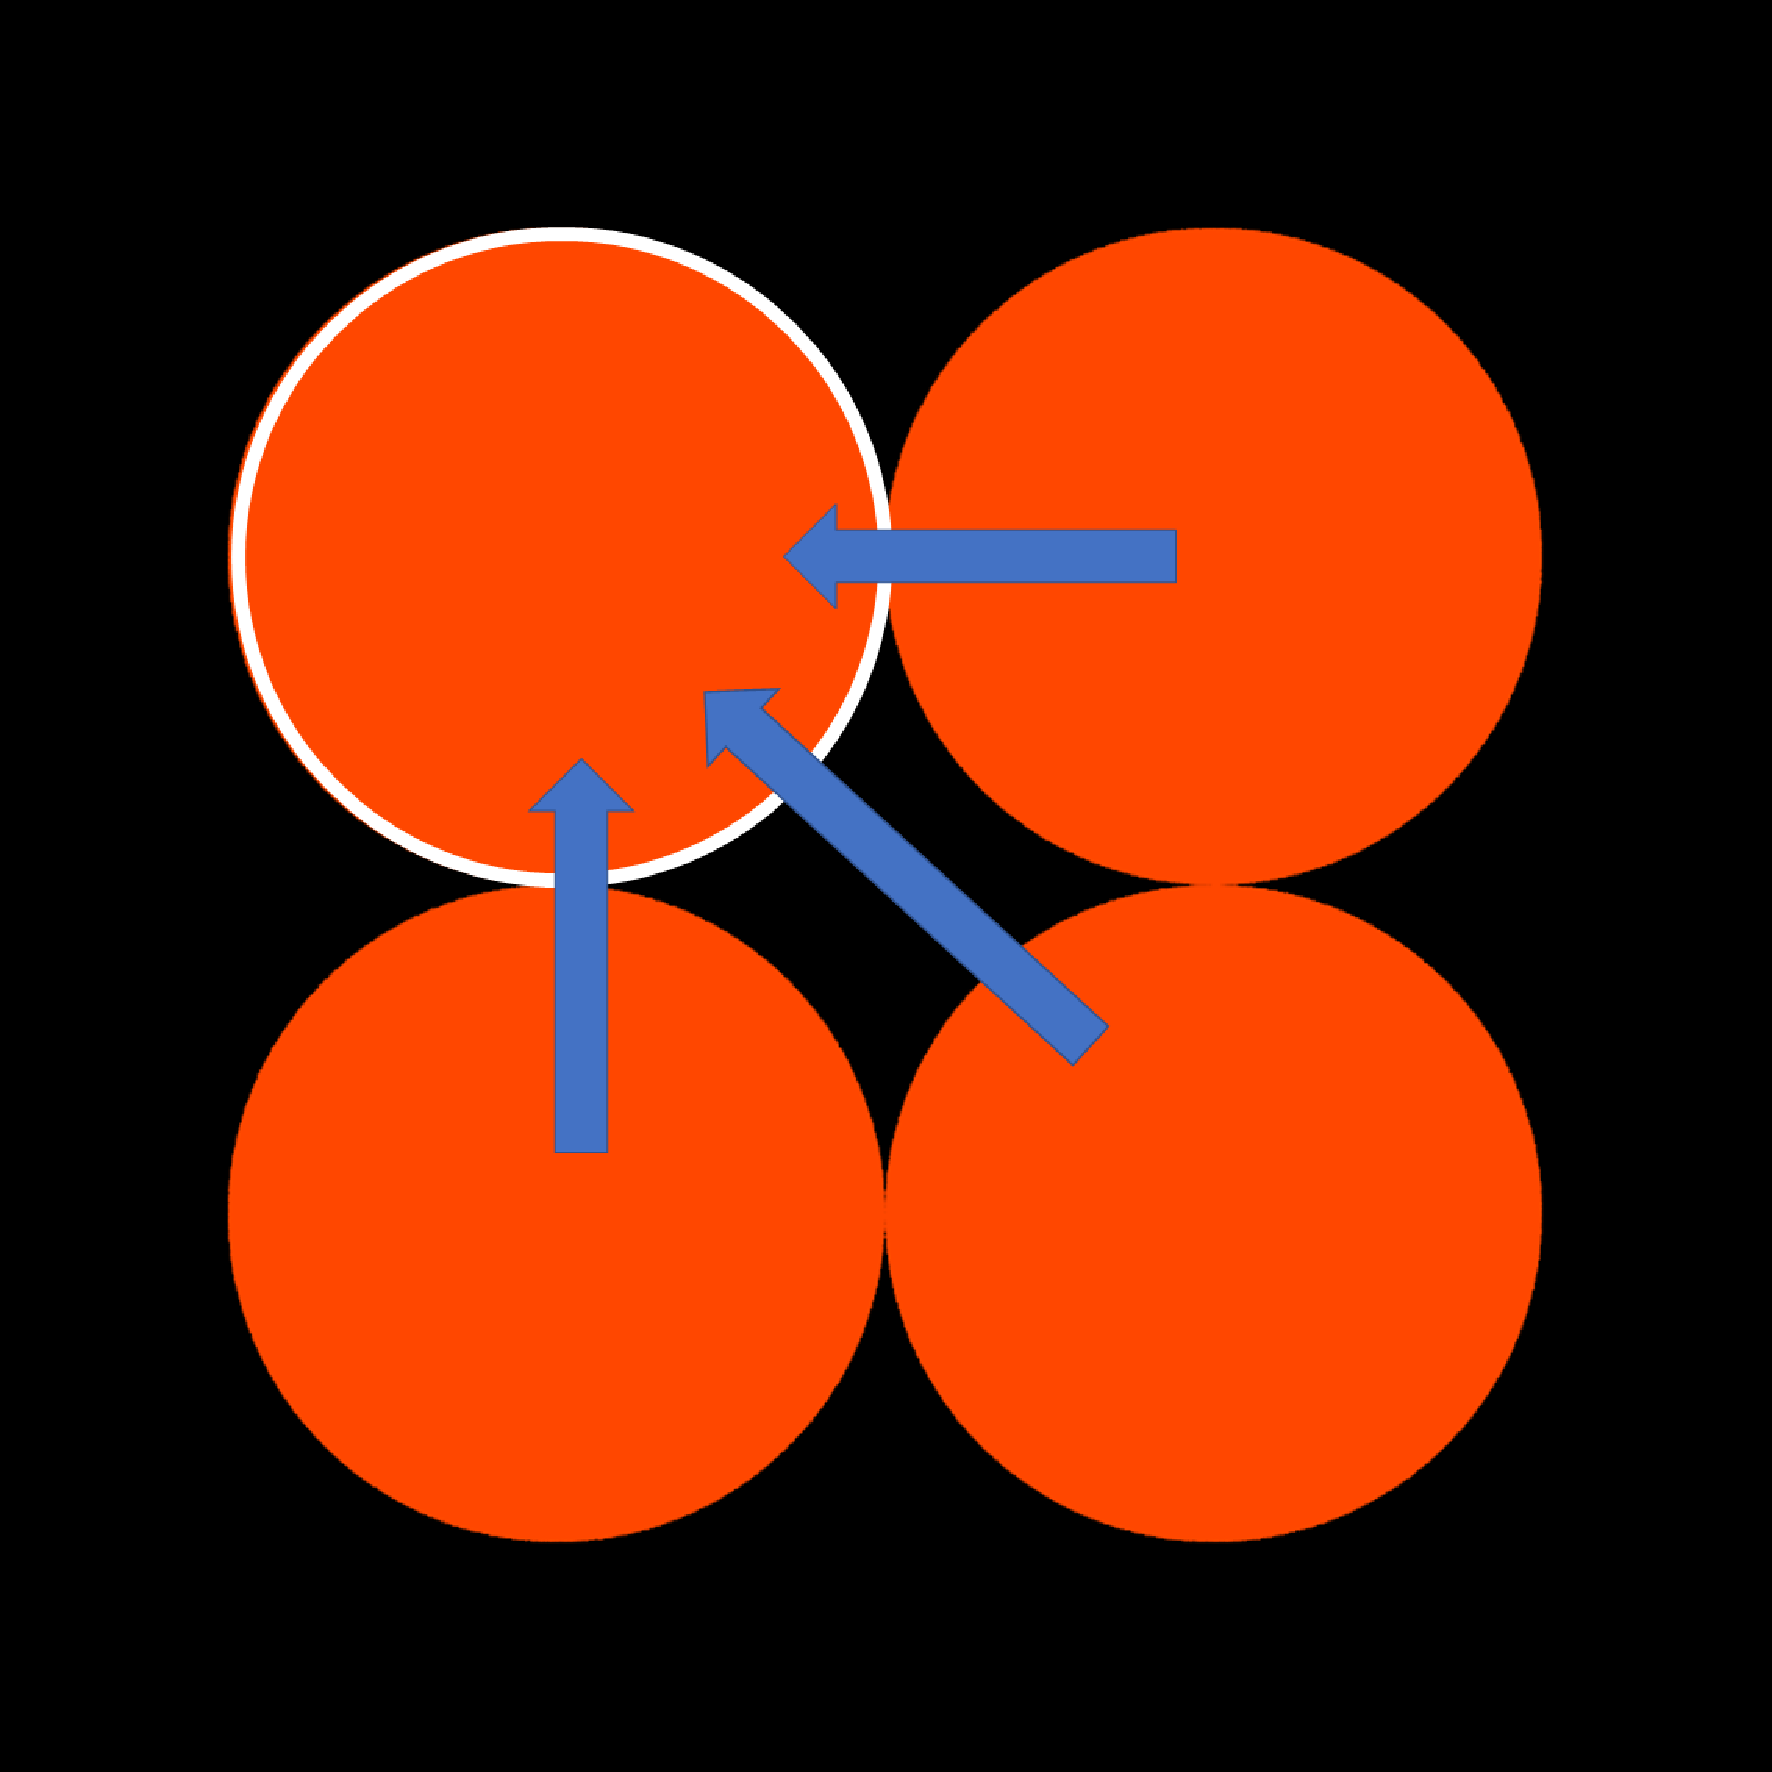
\includegraphics[width=2in, height=2in, keepaspectratio]{../img/klein/orbit/level0inv.pdf}
  \subcaption{}
   \label{fig:level0inv}
 \end{minipage}
 \begin{minipage}{0.33\hsize}
  \center
  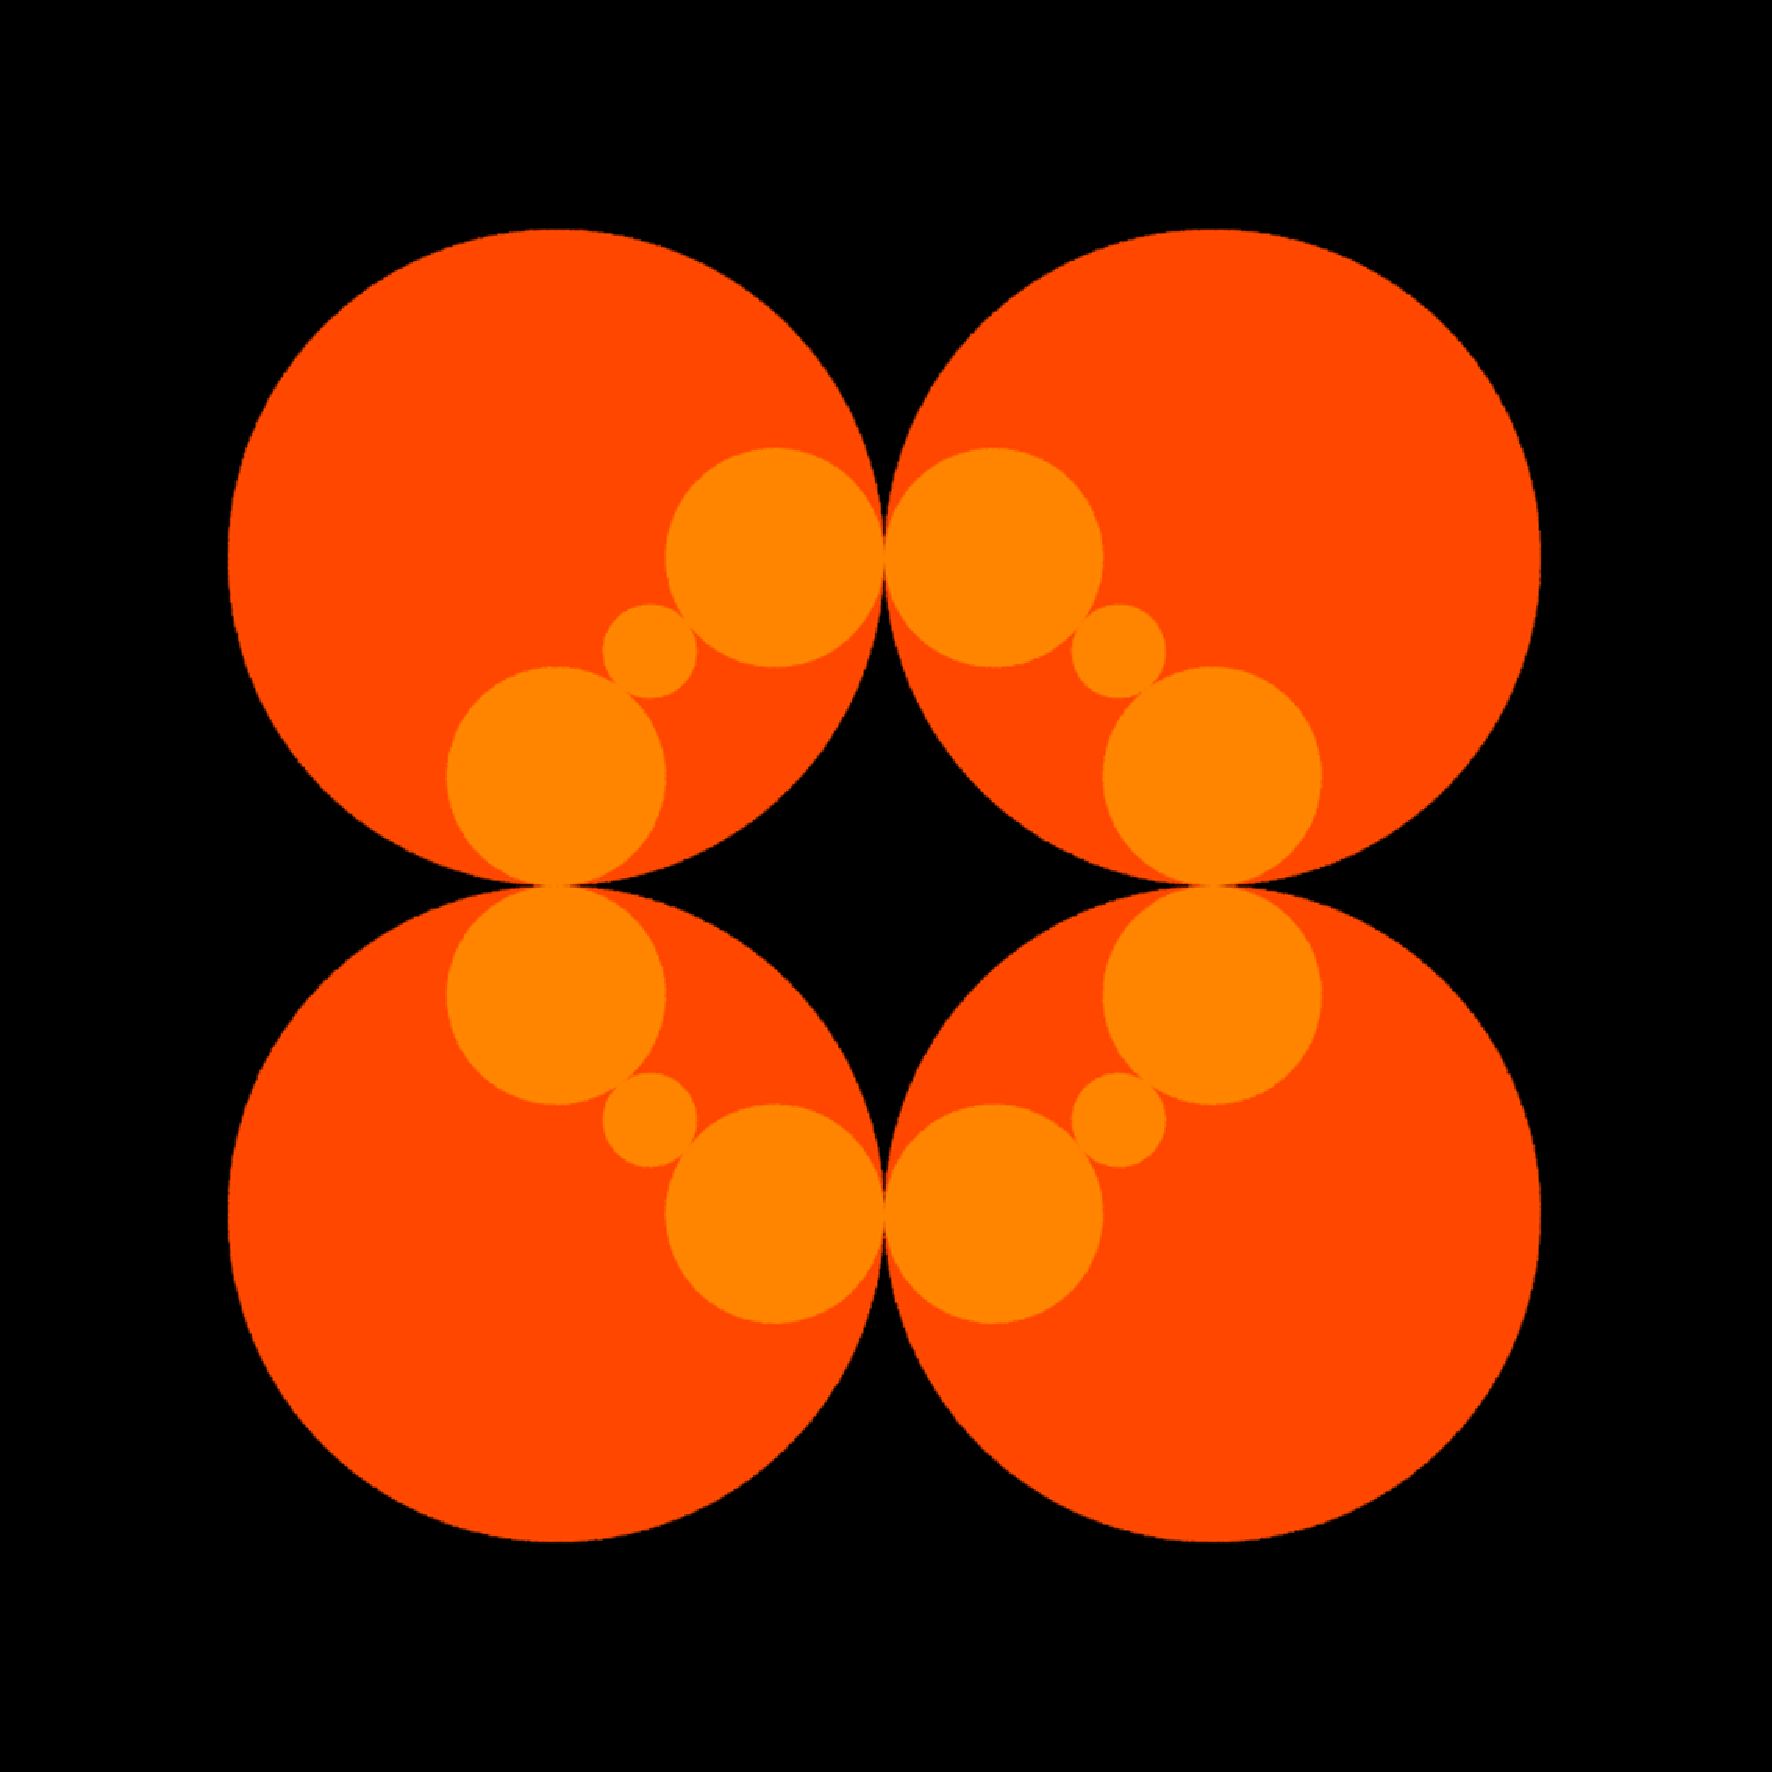
\includegraphics[width=2in, height=2in, keepaspectratio]{../img/klein/orbit/level1.pdf}
  \subcaption{}
   \label{fig:level1}
 \end{minipage}
 \begin{minipage}{0.33\hsize}
  \center
  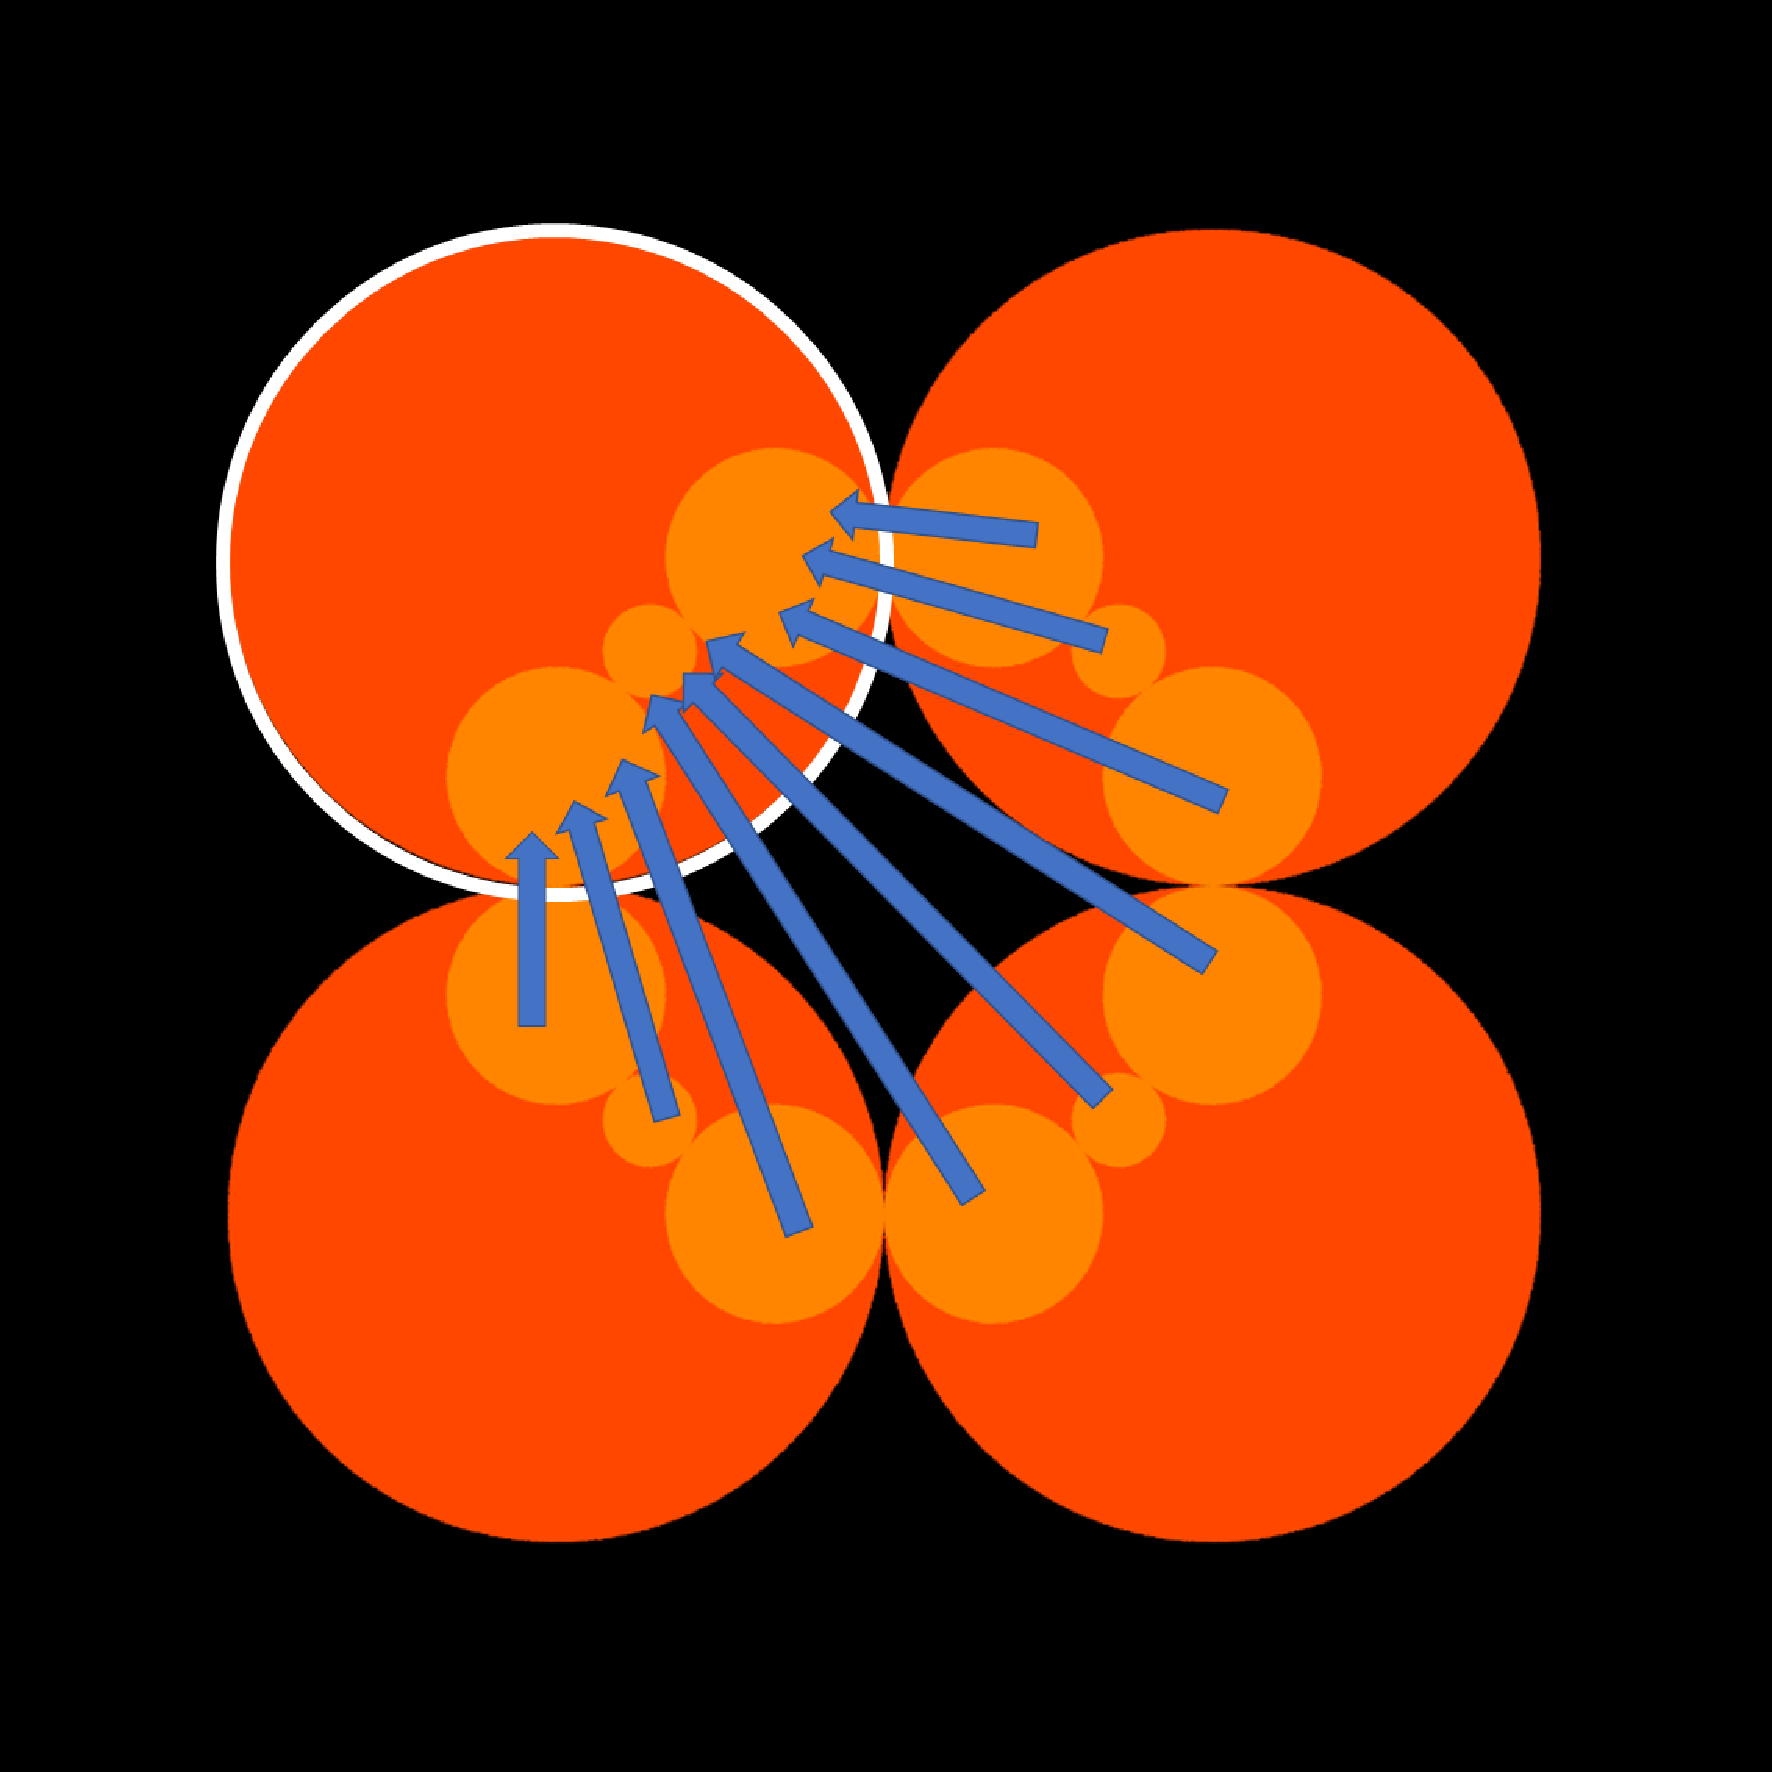
\includegraphics[width=2in, height=2in, keepaspectratio]{../img/klein/orbit/level1inv.pdf}
  \subcaption{}
  \label{fig:level1inv}
 \end{minipage}
 \begin{minipage}{0.33\hsize}
  \center
  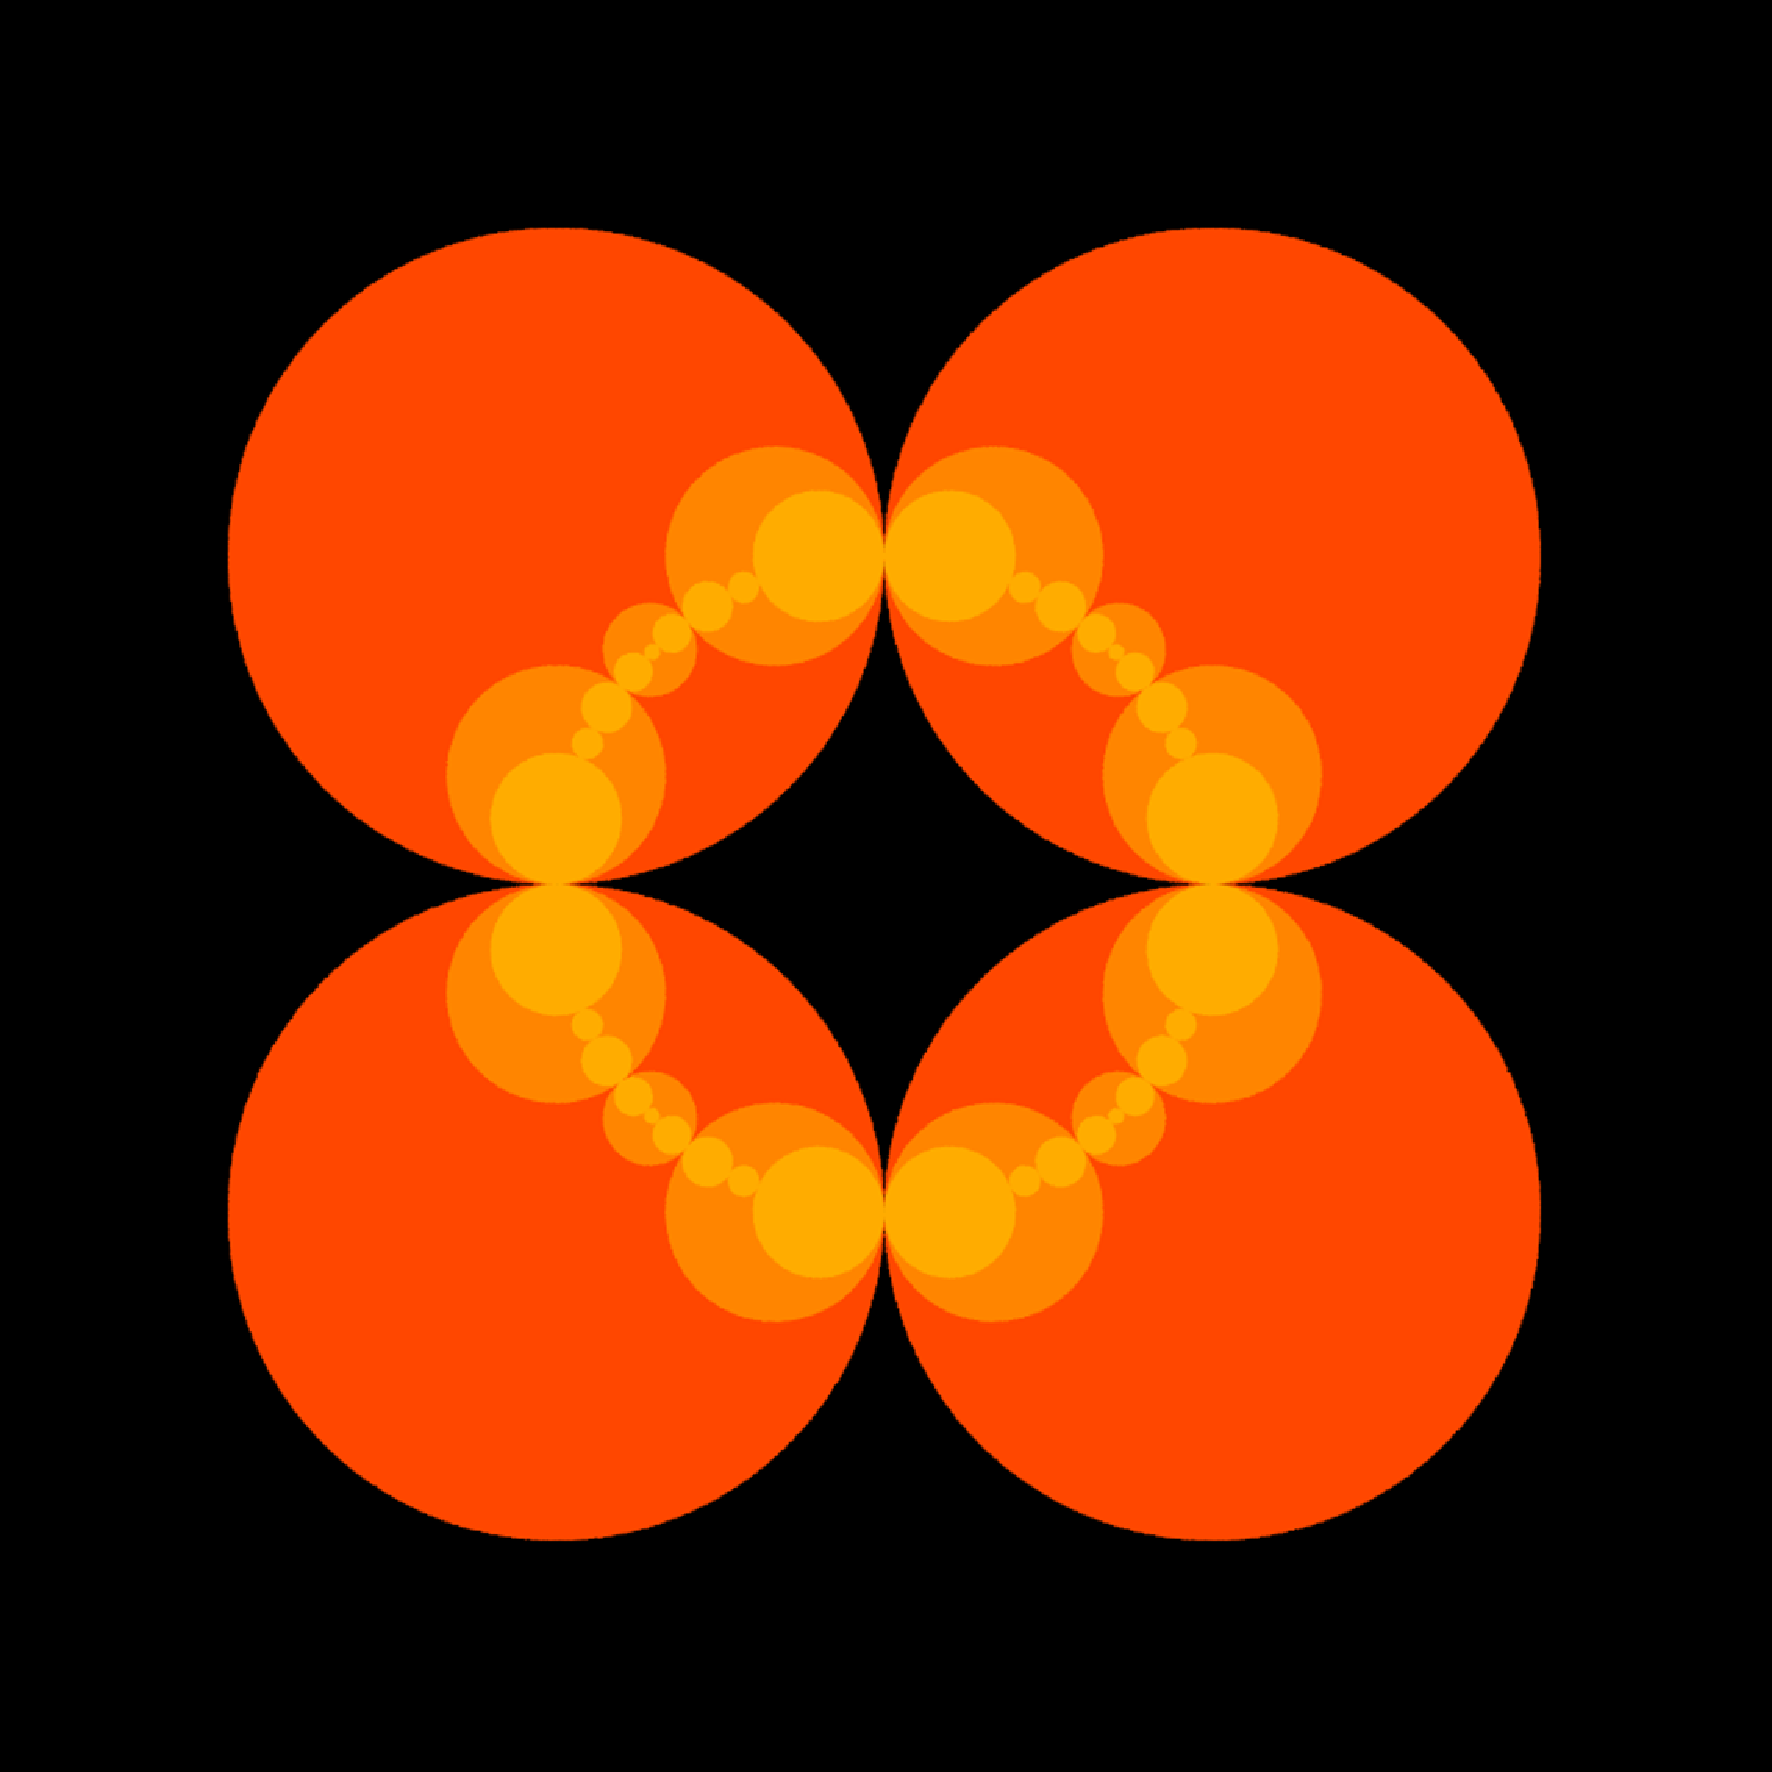
\includegraphics[width=2in, height=2in, keepaspectratio]{../img/klein/orbit/level2.pdf}
  \subcaption{}
  \label{fig:level2}
 \end{minipage}
 \begin{minipage}{0.33\hsize}
  \center
  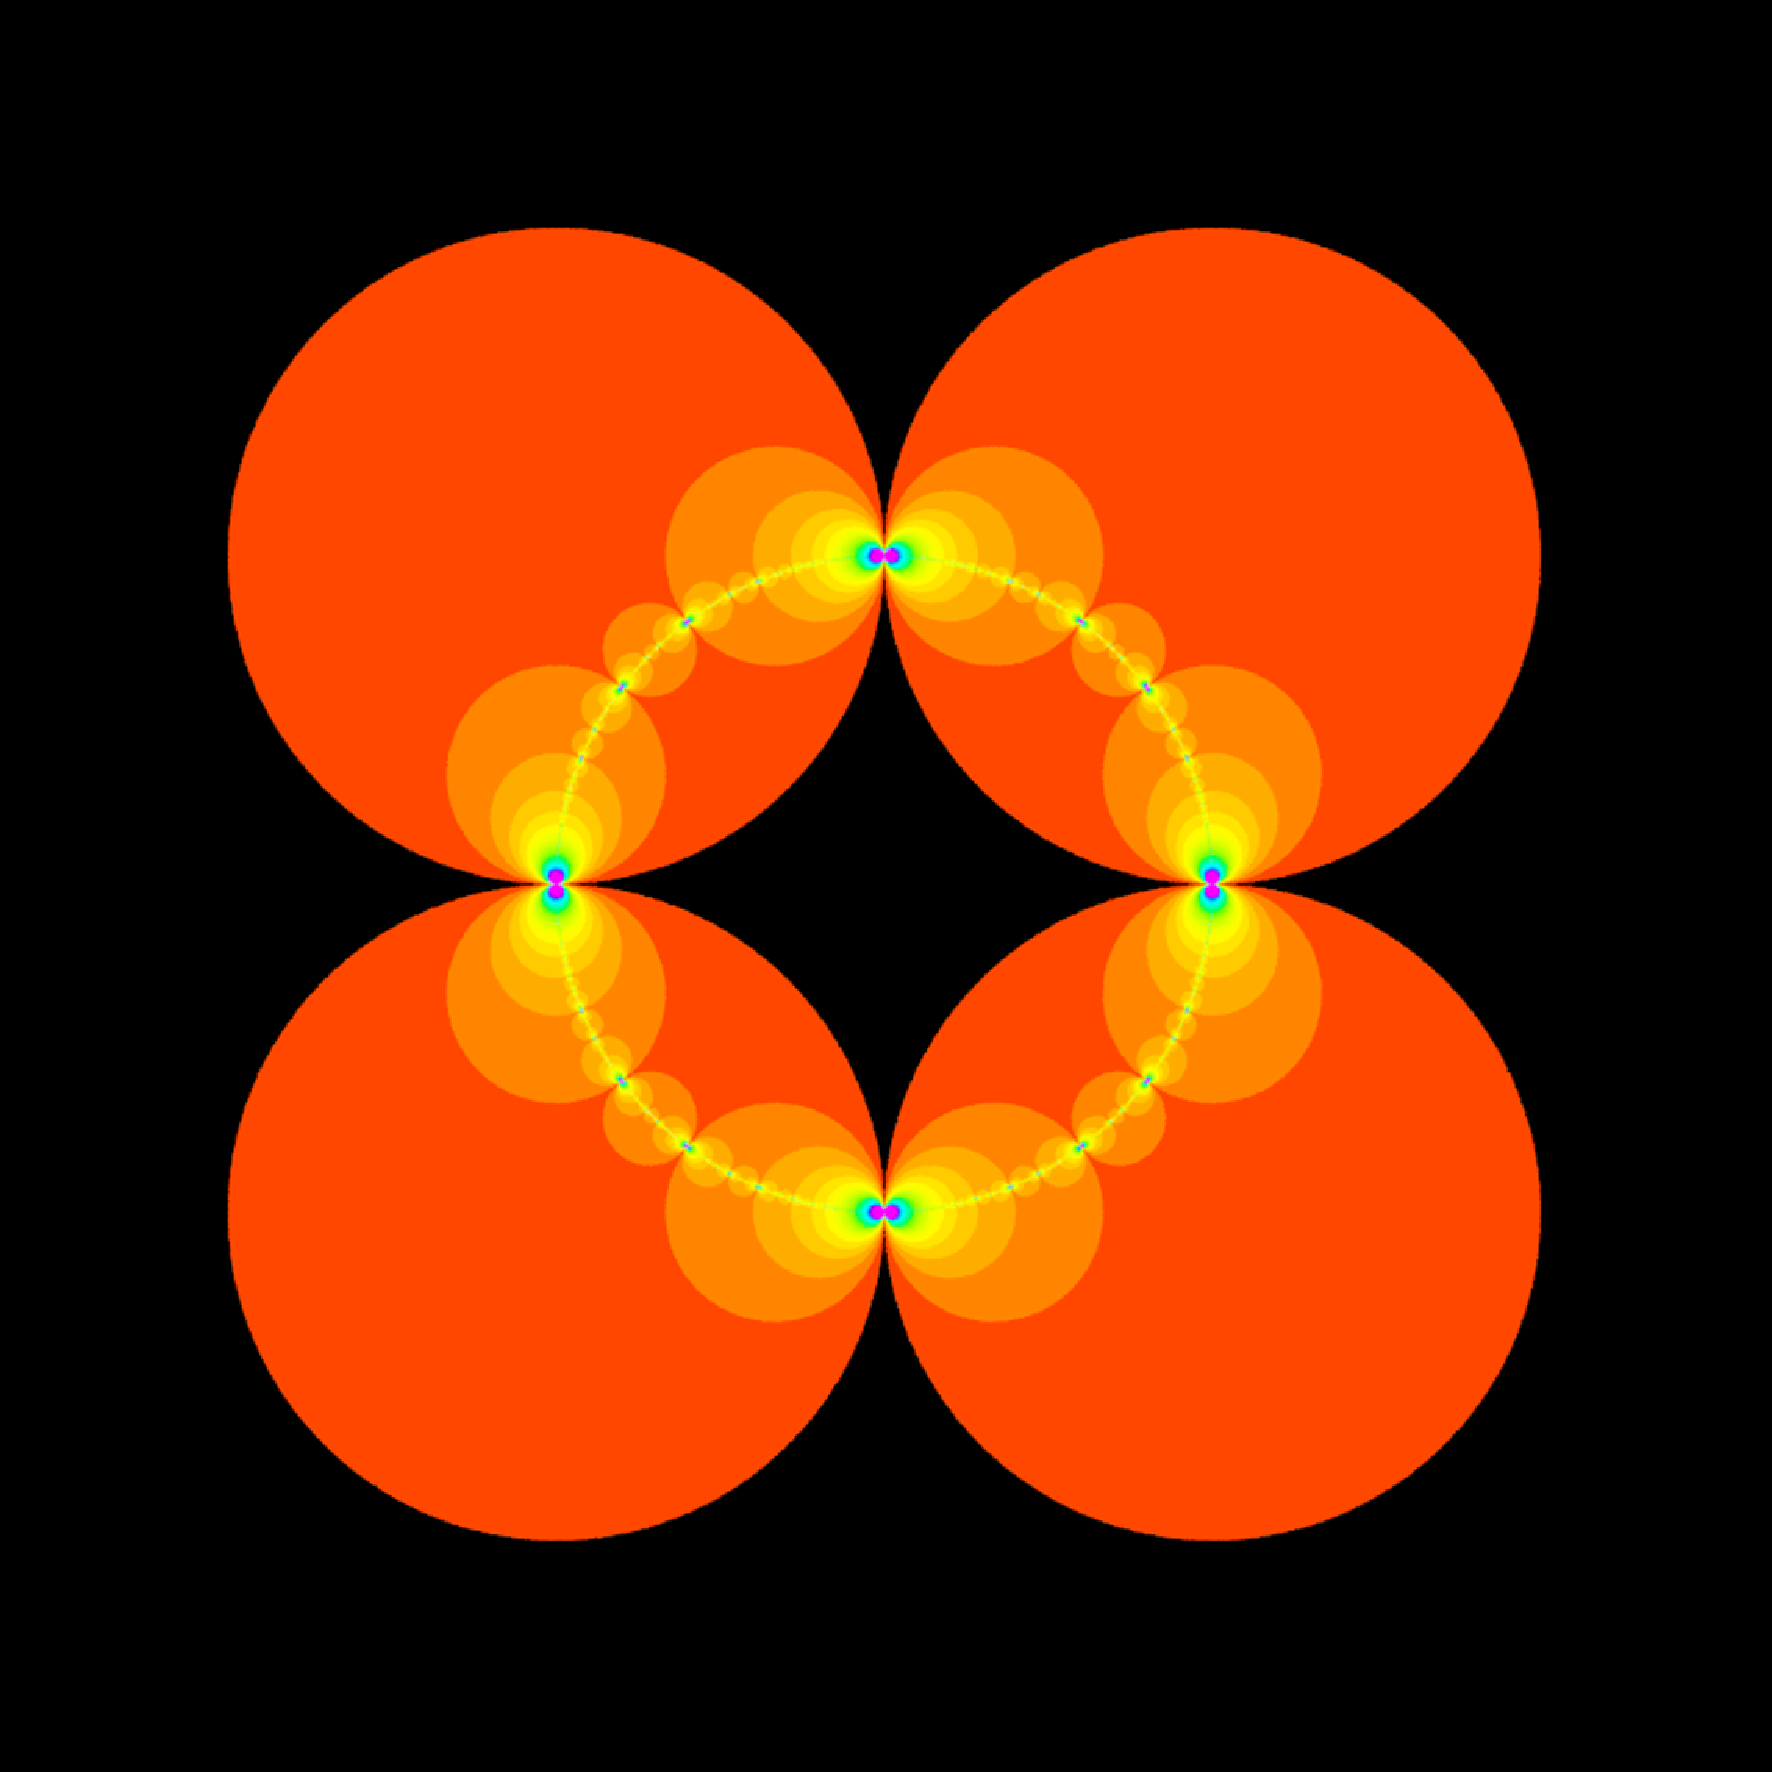
\includegraphics[width=2in, height=2in, keepaspectratio]{../img/klein/orbit/levelMax.pdf}
  \subcaption{}
  \label{fig:levelMax}
 \end{minipage}
 \caption{The process of rendering the orbit of circles}
\end{figure}

このアルゴリズムは変換で構成されるケーリーグラフを幅優先探索で探索するこ
とに等しい.
例えば,図\ref{fig:wordTree}の木を,語$a$のノードから時計回りに探索すると
$a,~b,~A,~B,~aB,~aa,~ab,~ba,~bb,~...$の順に合成された変換を得ることがで
きる.
あらかじめ決められた深さまで探索した後,得られたすべての合成変換を大本とな
る図形(図\ref{fig:orbit}においては中央の星)に対して作用させることで,その
図形の軌道を計算することができる.
このようにして描かれた図形の軌道をみることで,おおまかに生成元の作
用を観察することができる.

\subsubsection{Rendering the Limit Set}

群を可視化するためのもう一つの方法が,極限集合を描く方法である.
群の軌道を描く方法は,軌道の元となる図の位置によって得られる図が変わるこ
とや,計算量が大きいという欠点がある.
より複雑なメビウス変換群を可視化する際には極限集合を直接描く方法が使われる.

極限集合に含まれる点はケーリーグラフにおいて無限の深さのノードが表す合成変換に対応し
ている.しかし,現実にそれを求めることは不可能である.そこで,群の生成
元の固定点をある程度の長さをもった変換の語で移すことで極限集合に含まれる
点である極限点を求める.
例えば,変換$a$の固定点は任意の点に$a$を無限回作用させた点,つまり
$\overline{a}$を作用させた点と考えることができる.
そして,その点は極限集合に含まれる.
そのため,生成元の固定点を,グラフを探索して得られた合成変換で移すことで極
限集合に含まれる点を得ることができる.
一例を挙げると,合成変換$abbAAb\overline{a}$で表される点は$a$の固定点を合
成変換$abbAAb$で移すことで求めることができる.これも極限集合に含まれる.
このとき,$abbAAb$のように固定点に作用させる変換を\emph{接頭語}とよぶ.

接頭語を求める際には深さ優先探索が用いられる.
図\ref{fig:wordTree}の木を,語$a$のノードから時計回りに長さ3までの語を探索
すると$aBA,~aBB,~aBa,~aaB,~...$という順で接頭語が得られる.
これらの語に生成元の固定点を与えると極限点を求めることができる.
例えば,接頭語$aBA$を用いて$\overline{A},~\overline{b},~\overline{B}$の3つの固定
点を変換すると互いに近い3つの極限点が得られる.
$aab\overline{a}$と$aaa\overline{a}$のように隣同士の接頭語を持つ極限点や,
$aaa\overline{a}$と$aaa\overline{b}$のような同じ接頭語を持つ極限点同士は
近い位置にあることが証明されている.
そのため,得られた点同士を順番に結ぶと図\ref{fig:limitset}のようなフラクタル
構造を持つ曲線を得ることができる.
また,得られた点同士の距離によって,より深い語を探索するかどうかを判断し,
そこで計算を打ち切ることで探索を高速化することができる.

\begin{figure}[htbp]
 \begin{minipage}{0.5\hsize}
  \center
  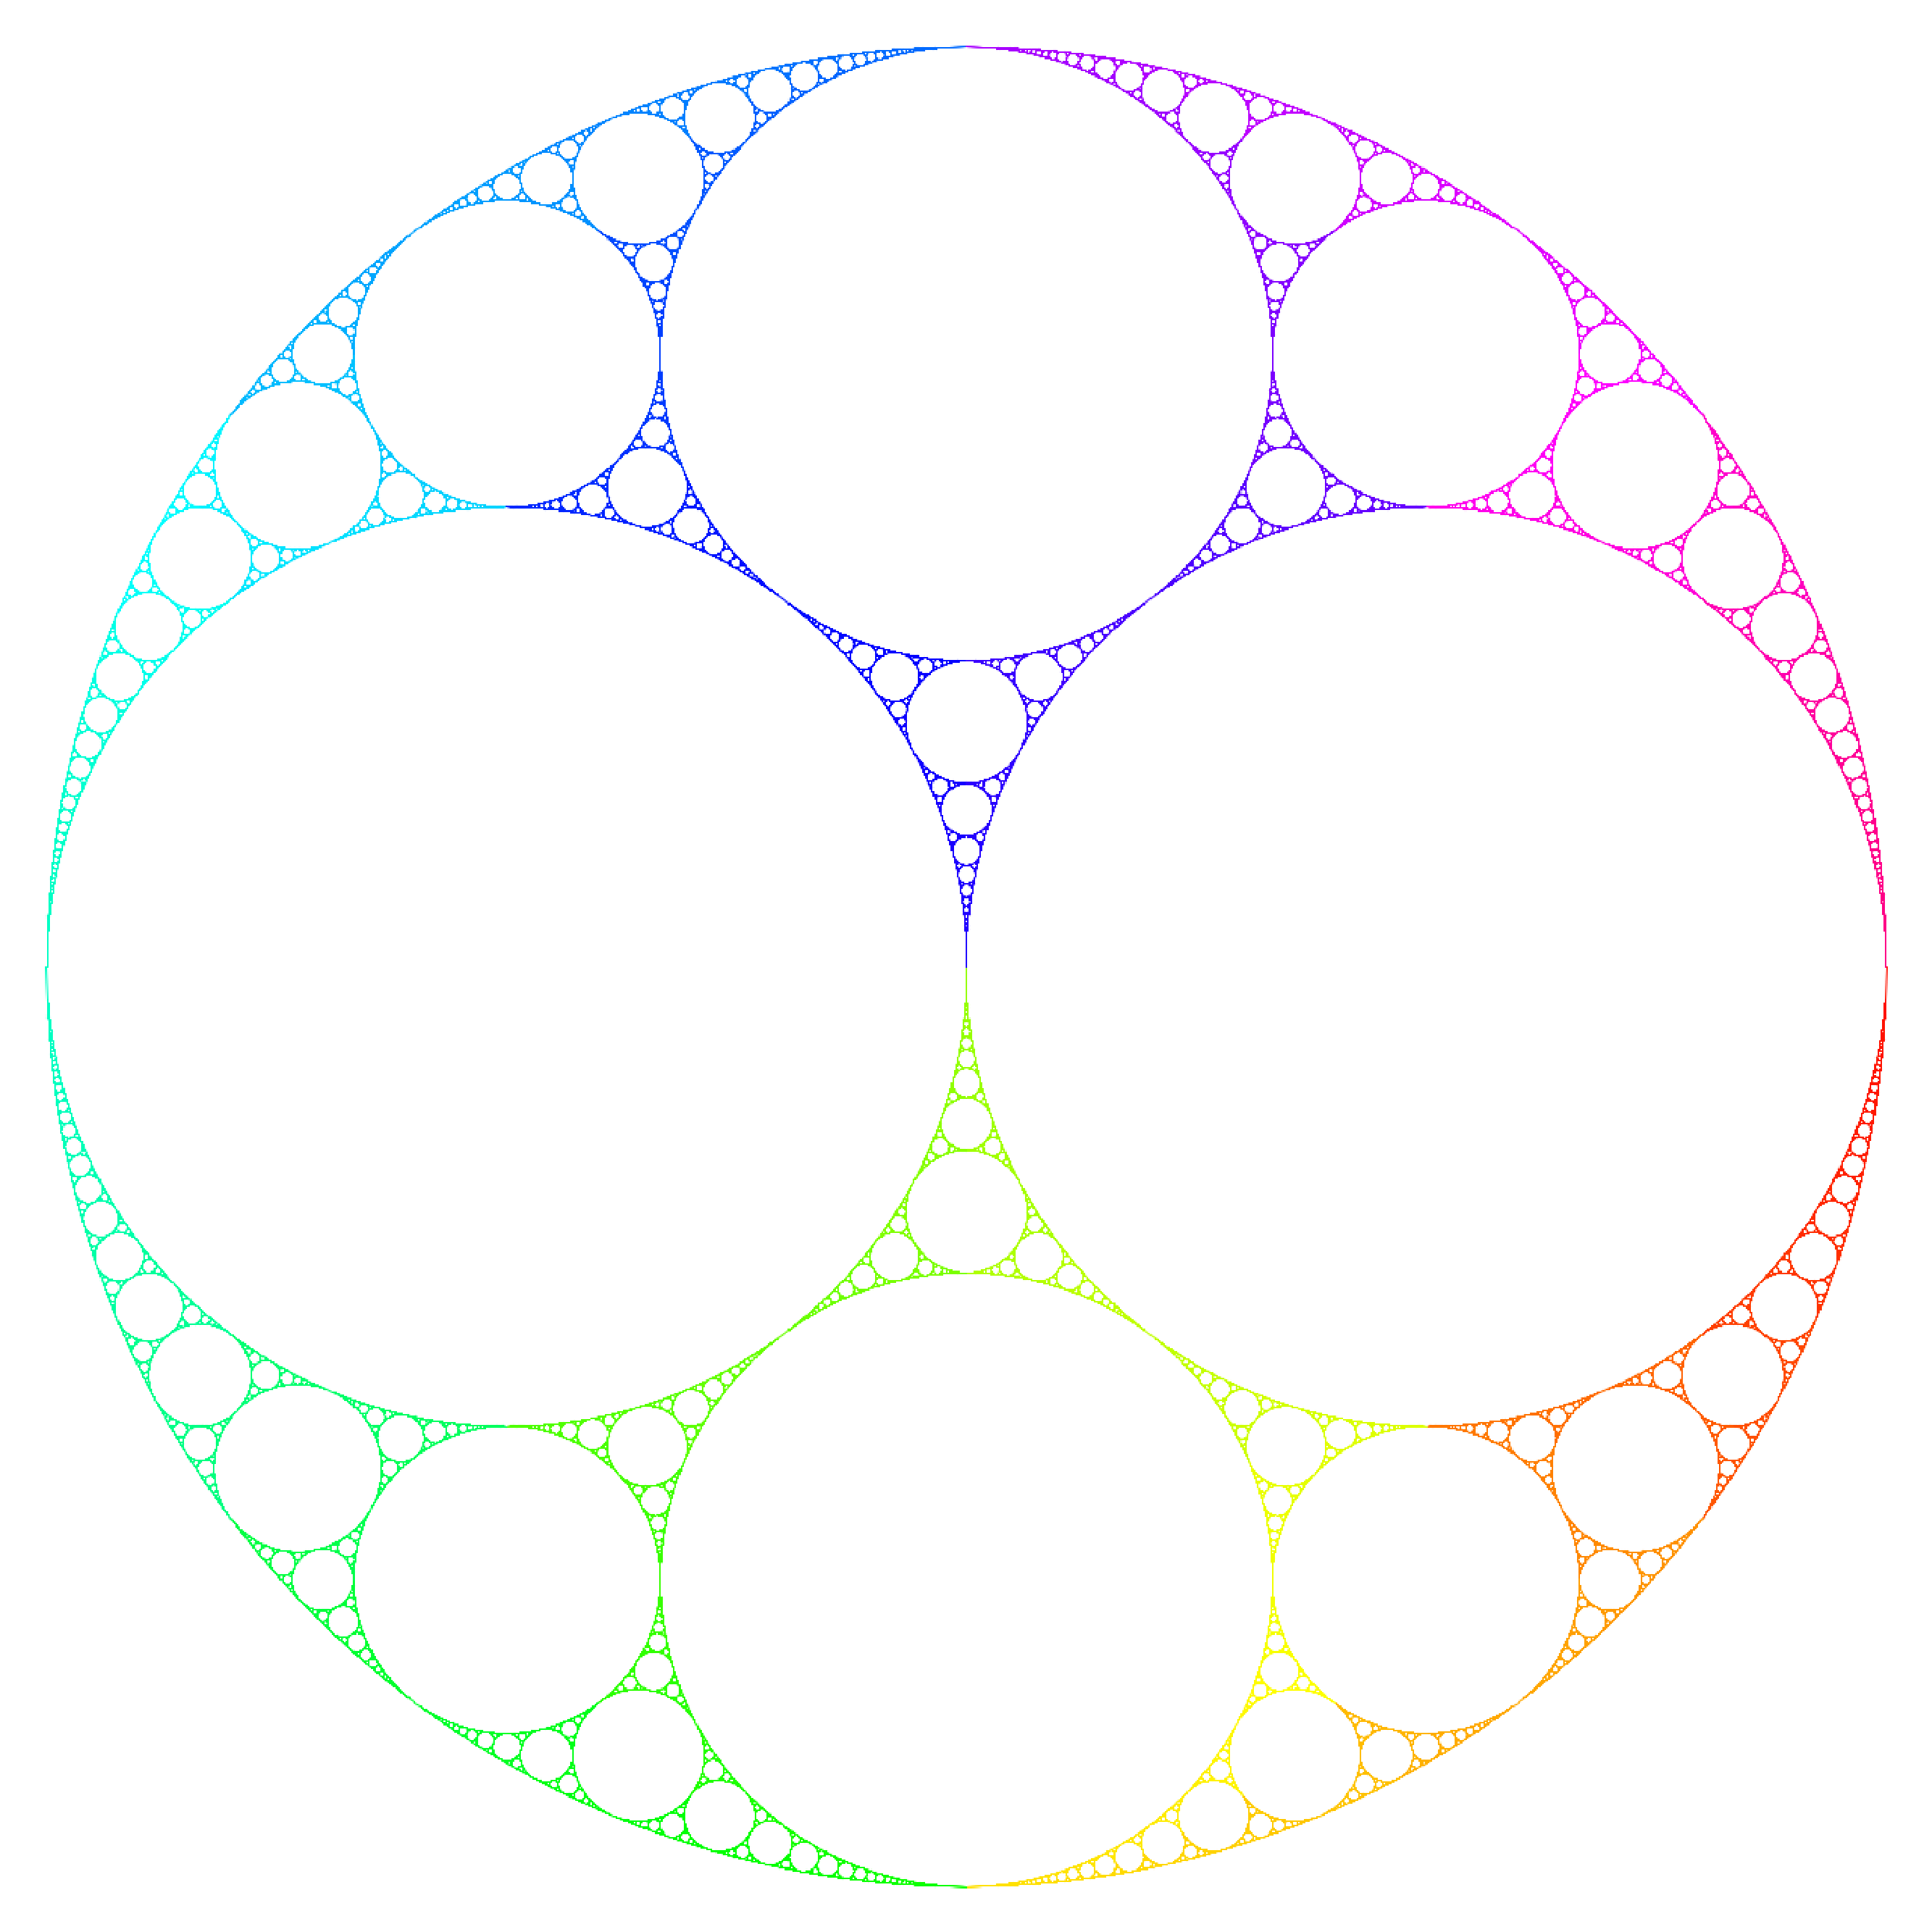
\includegraphics[ height=2.5in, keepaspectratio]{../img/klein/limitset/limit1.pdf}
  \subcaption{}
  \label{fig:limit1}
 \end{minipage}
 \begin{minipage}{0.5\hsize}
  \center
  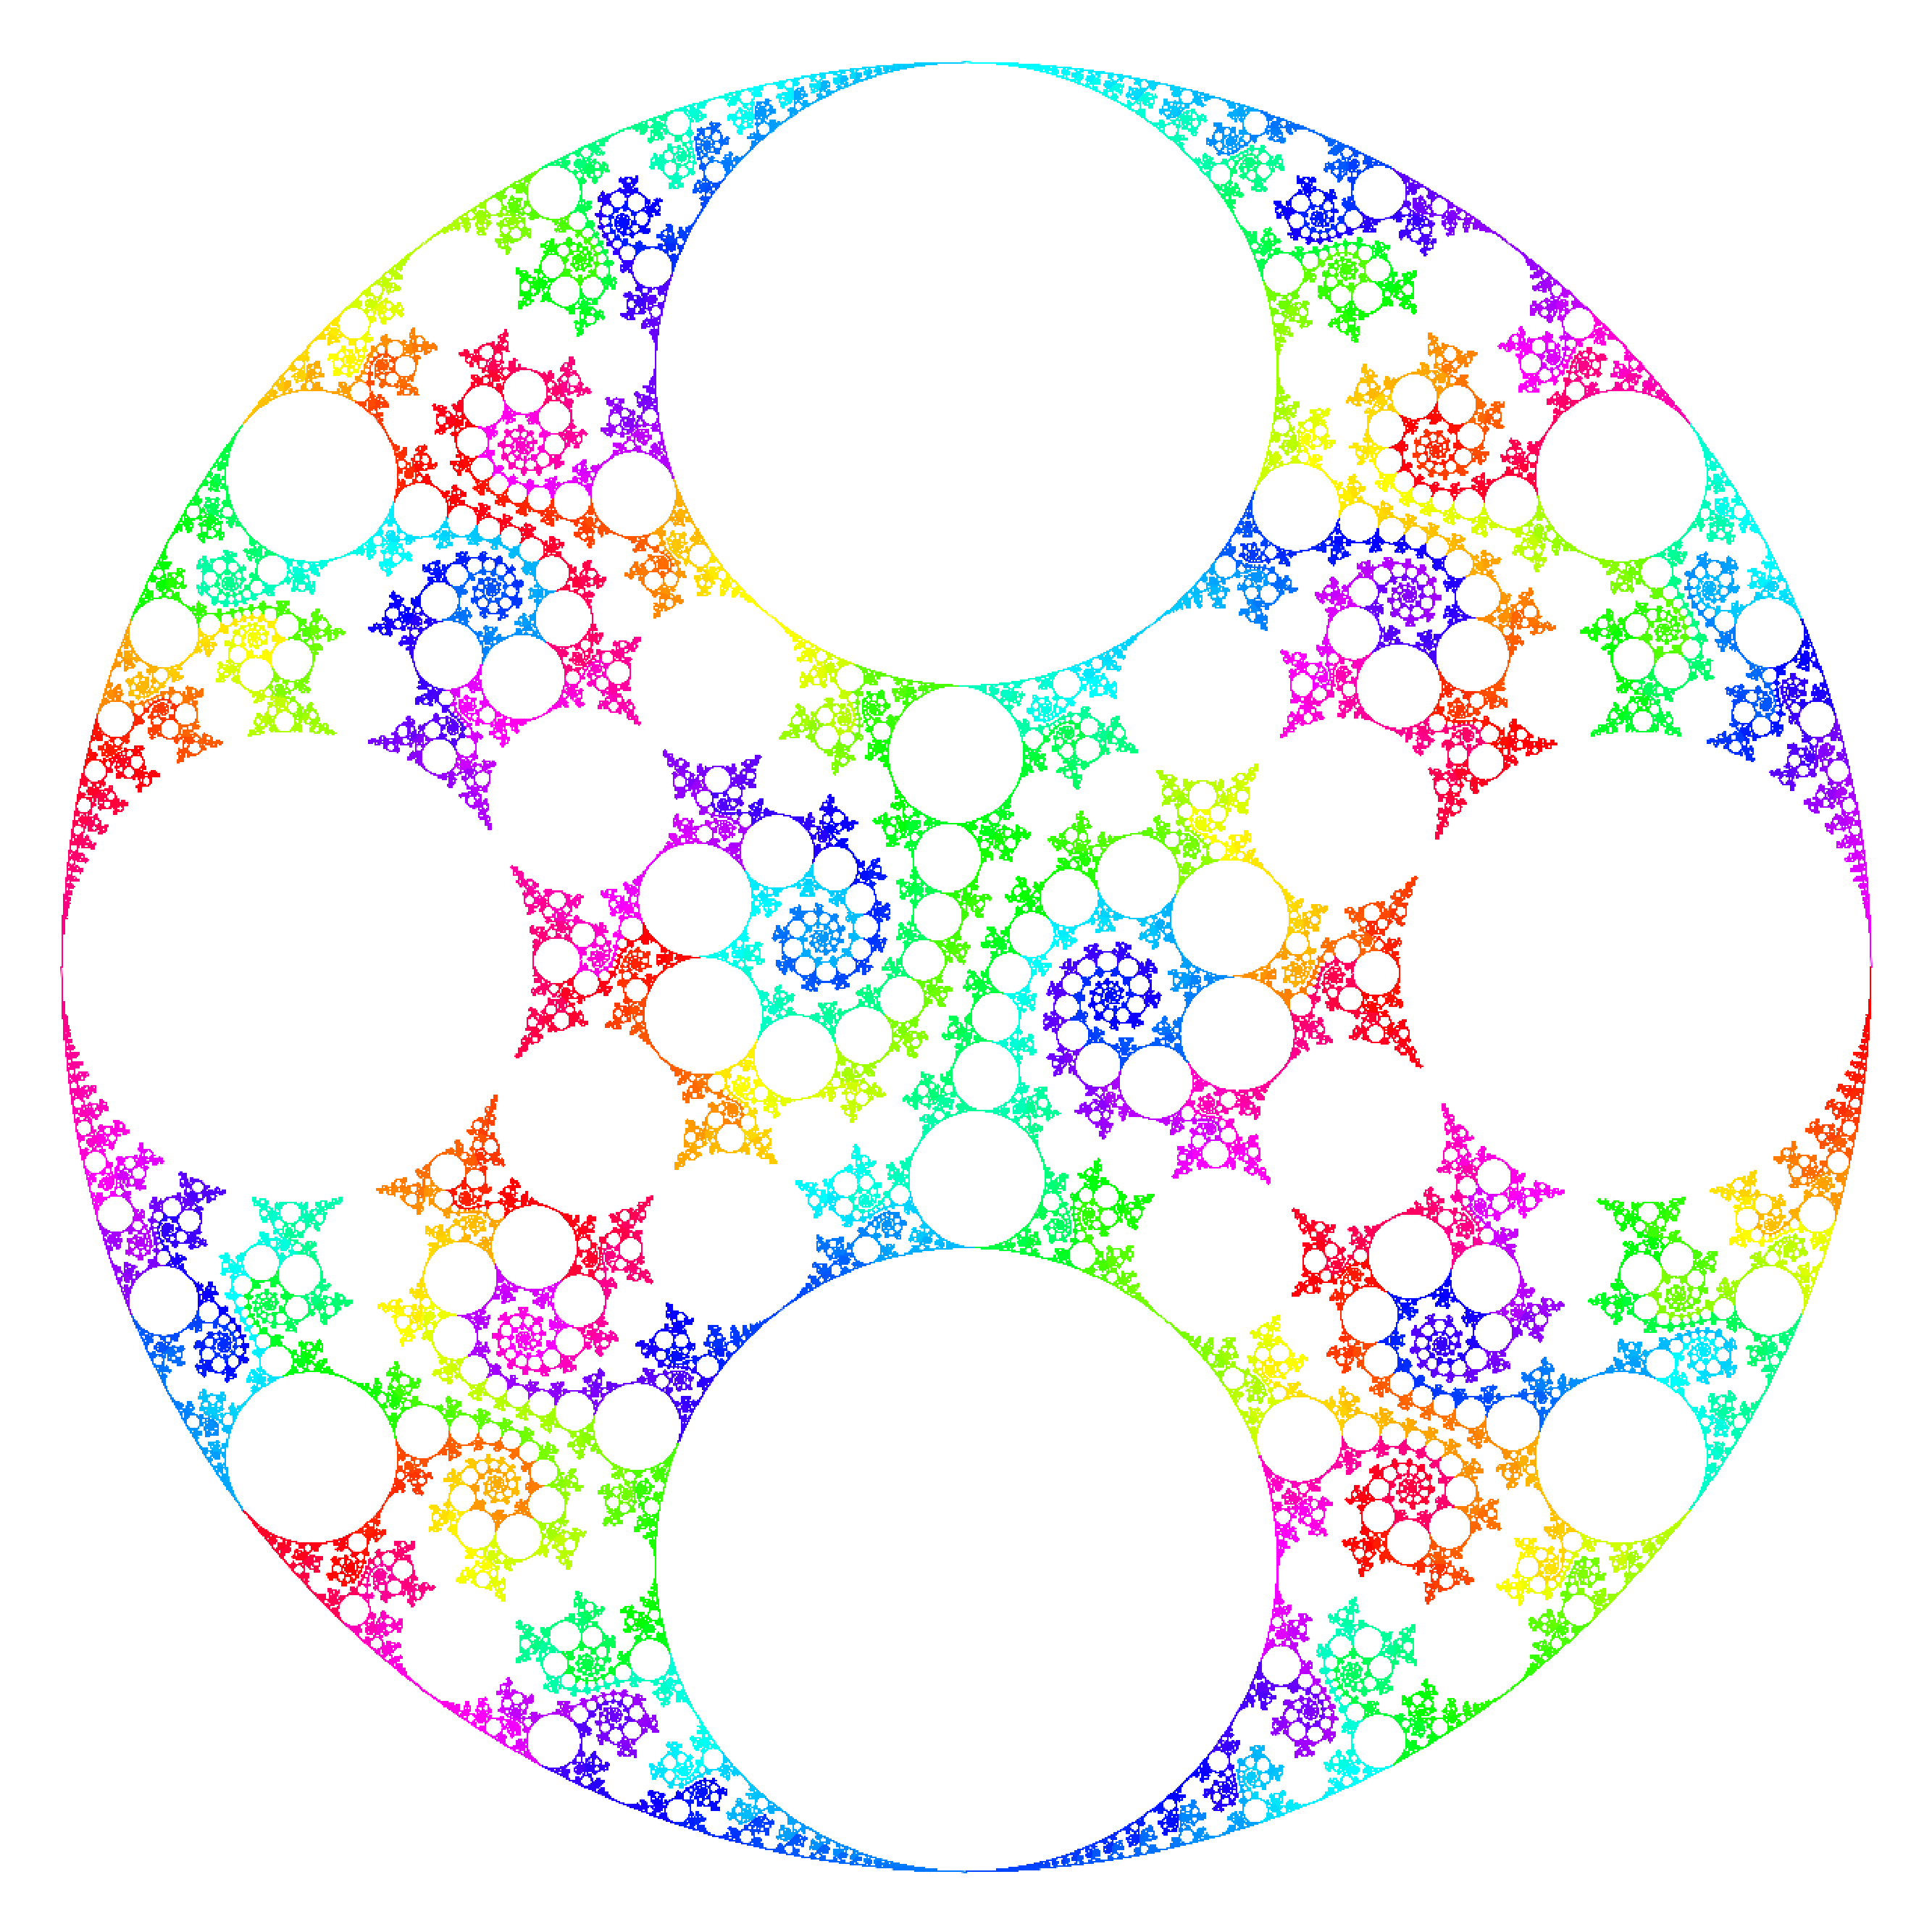
\includegraphics[ height=2.5in, keepaspectratio]{../img/klein/limitset/limit2.pdf}
  \subcaption{}
  \label{fig:limit2}
 \end{minipage}
 \begin{minipage}{0.5\hsize}
  \center
  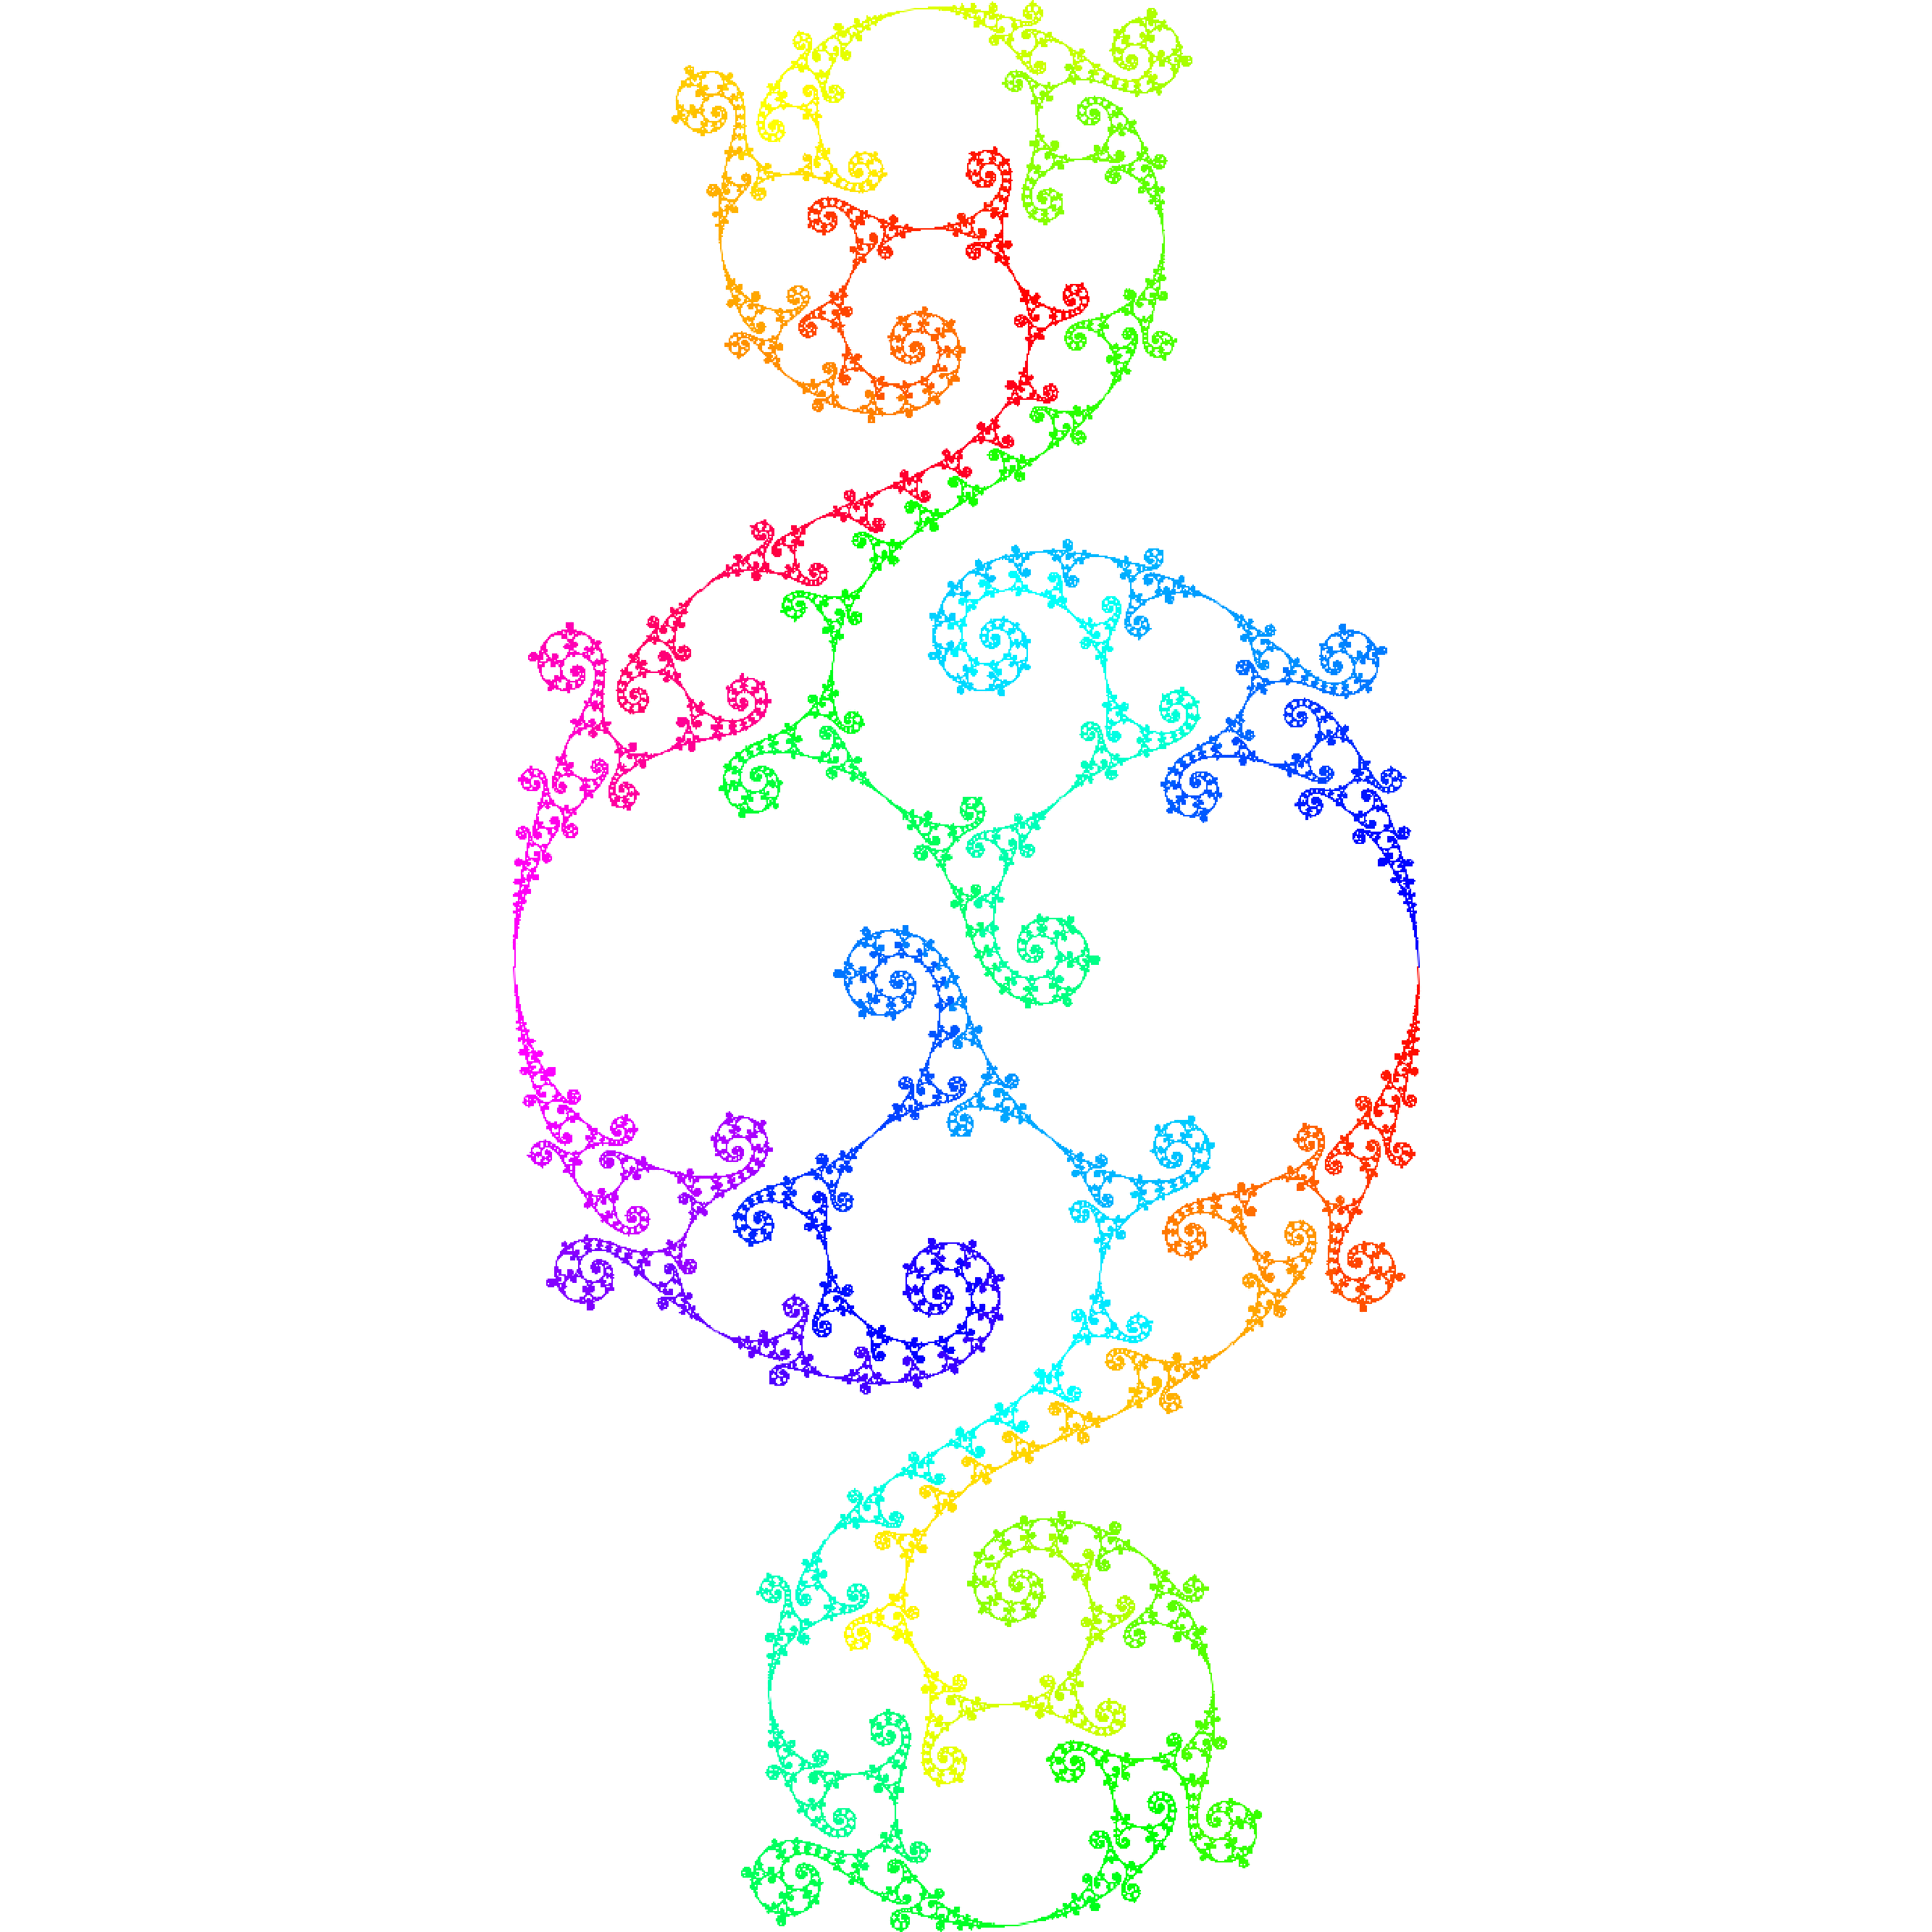
\includegraphics[ height=2.5in, keepaspectratio]{../img/klein/limitset/limit3.pdf}
  \subcaption{}
  \label{fig:limit3}
 \end{minipage}
 \begin{minipage}{0.5\hsize}
  \center
  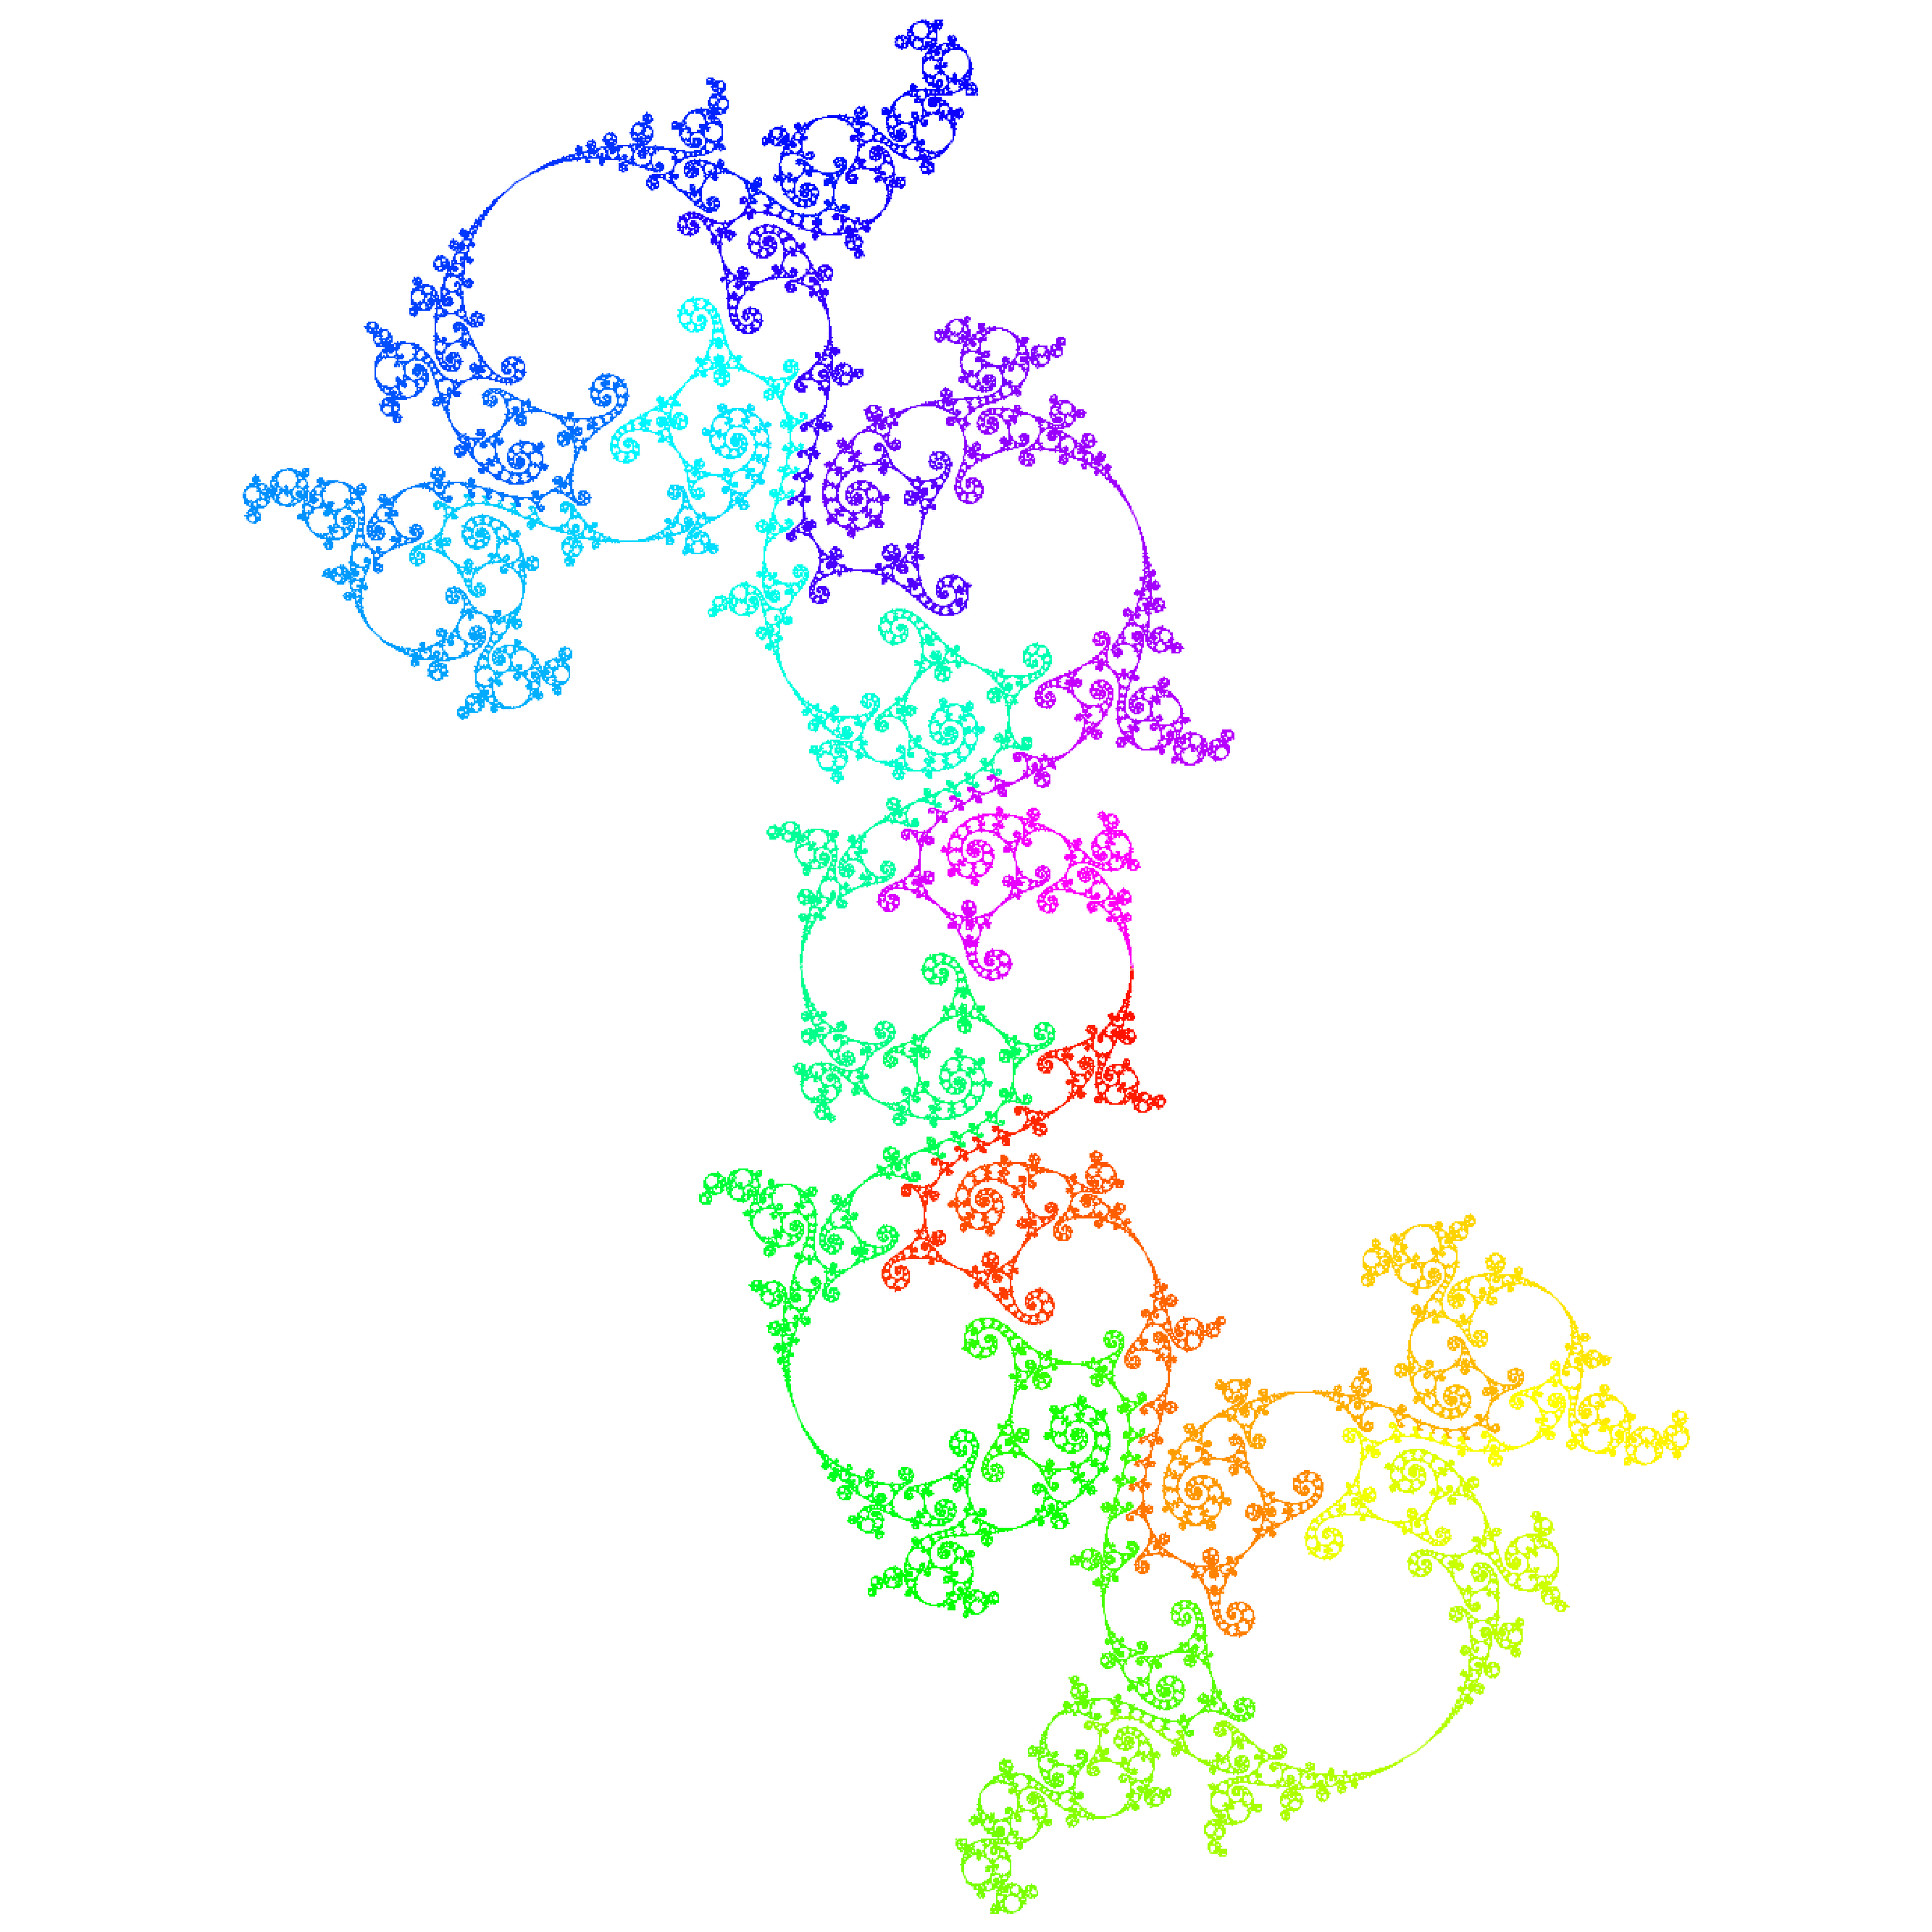
\includegraphics[ height=2.5in, keepaspectratio]{../img/klein/limitset/limit4.pdf}
  \subcaption{}
  \label{fig:limit4}
 \end{minipage}
 \caption{The limit set of Kleinian groups}
 \label{fig:limitset}
\end{figure}

ここまでに述べた方法のみで,極限集合を描画することは可能であるが,
より綺麗に,高速に描画するためには様々な工夫が必要となる.
例えば,放物型変換は固定点への収束に時間がかかるため,放物型変換の固定点付近
をうまく描画するためにグラフを深く探索しなければならない.
図\ref{fig:limit1}の右端をよく見ると直線で結ばれていることがわかる.
ここには放物型変換の固定点が存在しており収束が遅い.
そのため,この近辺の極限点を得るためにはより長い接頭語が必要となる.
『インドラの真珠』では放物型の生成元を特別視して扱う「特殊語アルゴリズム」と
よばれるアルゴリズムを用いることで.固定点近辺を直線で描くことで探索を効
率化する.

また,ある変換とその逆変換を合成してしまうと恒等変換になってしまうことは
自明であるが,特定の変換の組み合わせが恒等変換を生み出してしまうことがある.
例えば,語$a$を$f(z) = z + 1$,語$b$を$g(z) = z + i$とするとき,
abABという語が表す合成変換は恒等変換となってしまう.
このような語を$\dot{も}\dot{た}\dot{な}\dot{い}$群を\emph{自由群}と呼ぶ.
こういった語が存在するとケーリーグラフの探索の効率が悪くなってしまうた
め,これらを取り除く必要がある.
これには有限オートマトンが使われる.
有限オートマトンに関しては,ここで扱わないので『インドラの真珠』を参照されたい.
また,変換群に関する有限オートマトンを取り扱った書籍には\textit{Word
Processing InGroups}~\cite{Epstein:1992:wordProcessing}がある.

先に述べたように,メビウス変換群の離散部分群がクライン群となる.
群の中には描画すると極限集合が収束せず,図\ref{fig:non-discrete}
のように乱れるものがある.
このような群は\emph{非離散群}とよばれ,クライン群ではない.
メビウス変換群のなかで,どのようなパラメータを持つ群が離散的であるか,す
なわちクライン群となるかを調べることがクライン群の研究テーマの一つとなる.
離散,非離散を判定するために有用な定理として\emph{ポアンカレの多面体定理}
や\emph{ヨルゲンセン不等式定理}とよばれるものが存在する.

離散と非離散のパラメータ領域を描画した図は\emph{スライス}とよばれ,
スライスの離散と非離散の境界もしばしばフラクタル形状となる.
また,その境界付近のパラメータの群を描画すると極限集合がしばしば興味
深い形になる.
山下のウェブページ\footnote{Discreteness Locus:
\url{http://vivaldi.ics.nara-wu.ac.jp/~yamasita/Slice/}}では様々な
スライスの画像を見ることができる.

\begin{figure}[htbp]
 \begin{minipage}{0.5\hsize}
  \center
  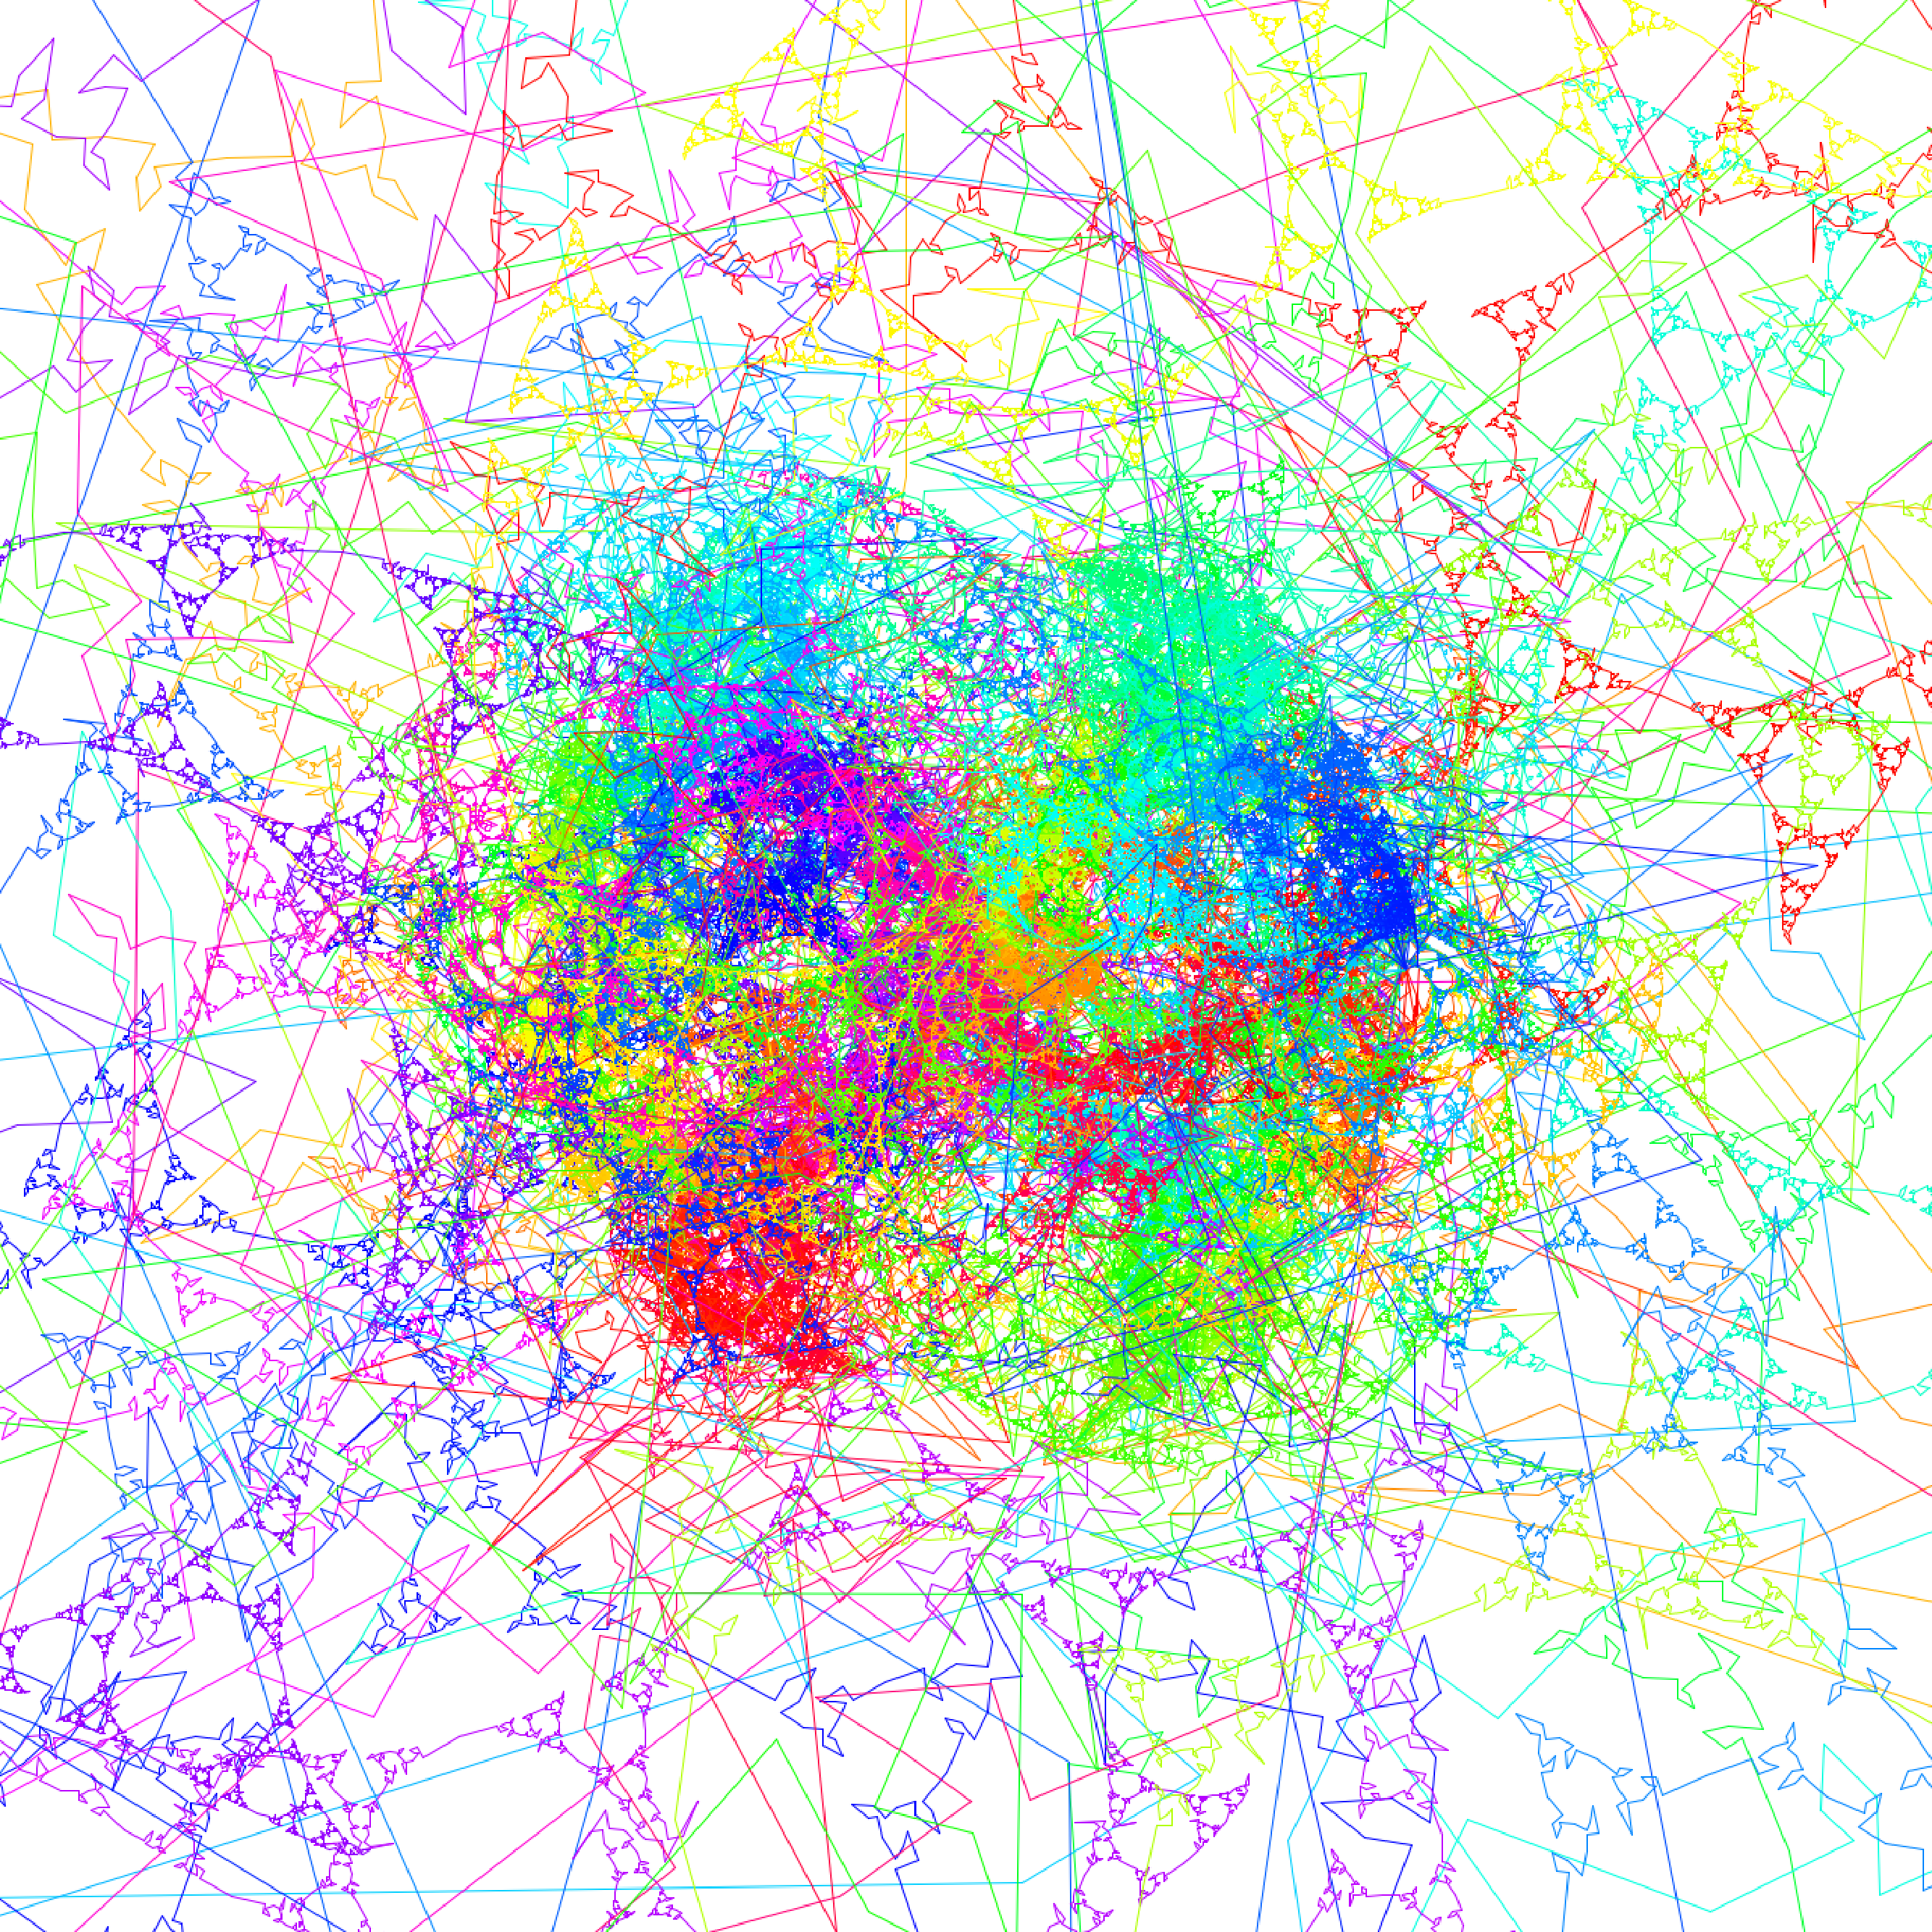
\includegraphics[ height=2.5in, keepaspectratio]{../img/klein/limitset/non-discrete1.pdf}
  \subcaption{}
 \end{minipage}
 \begin{minipage}{0.5\hsize}
  \center
  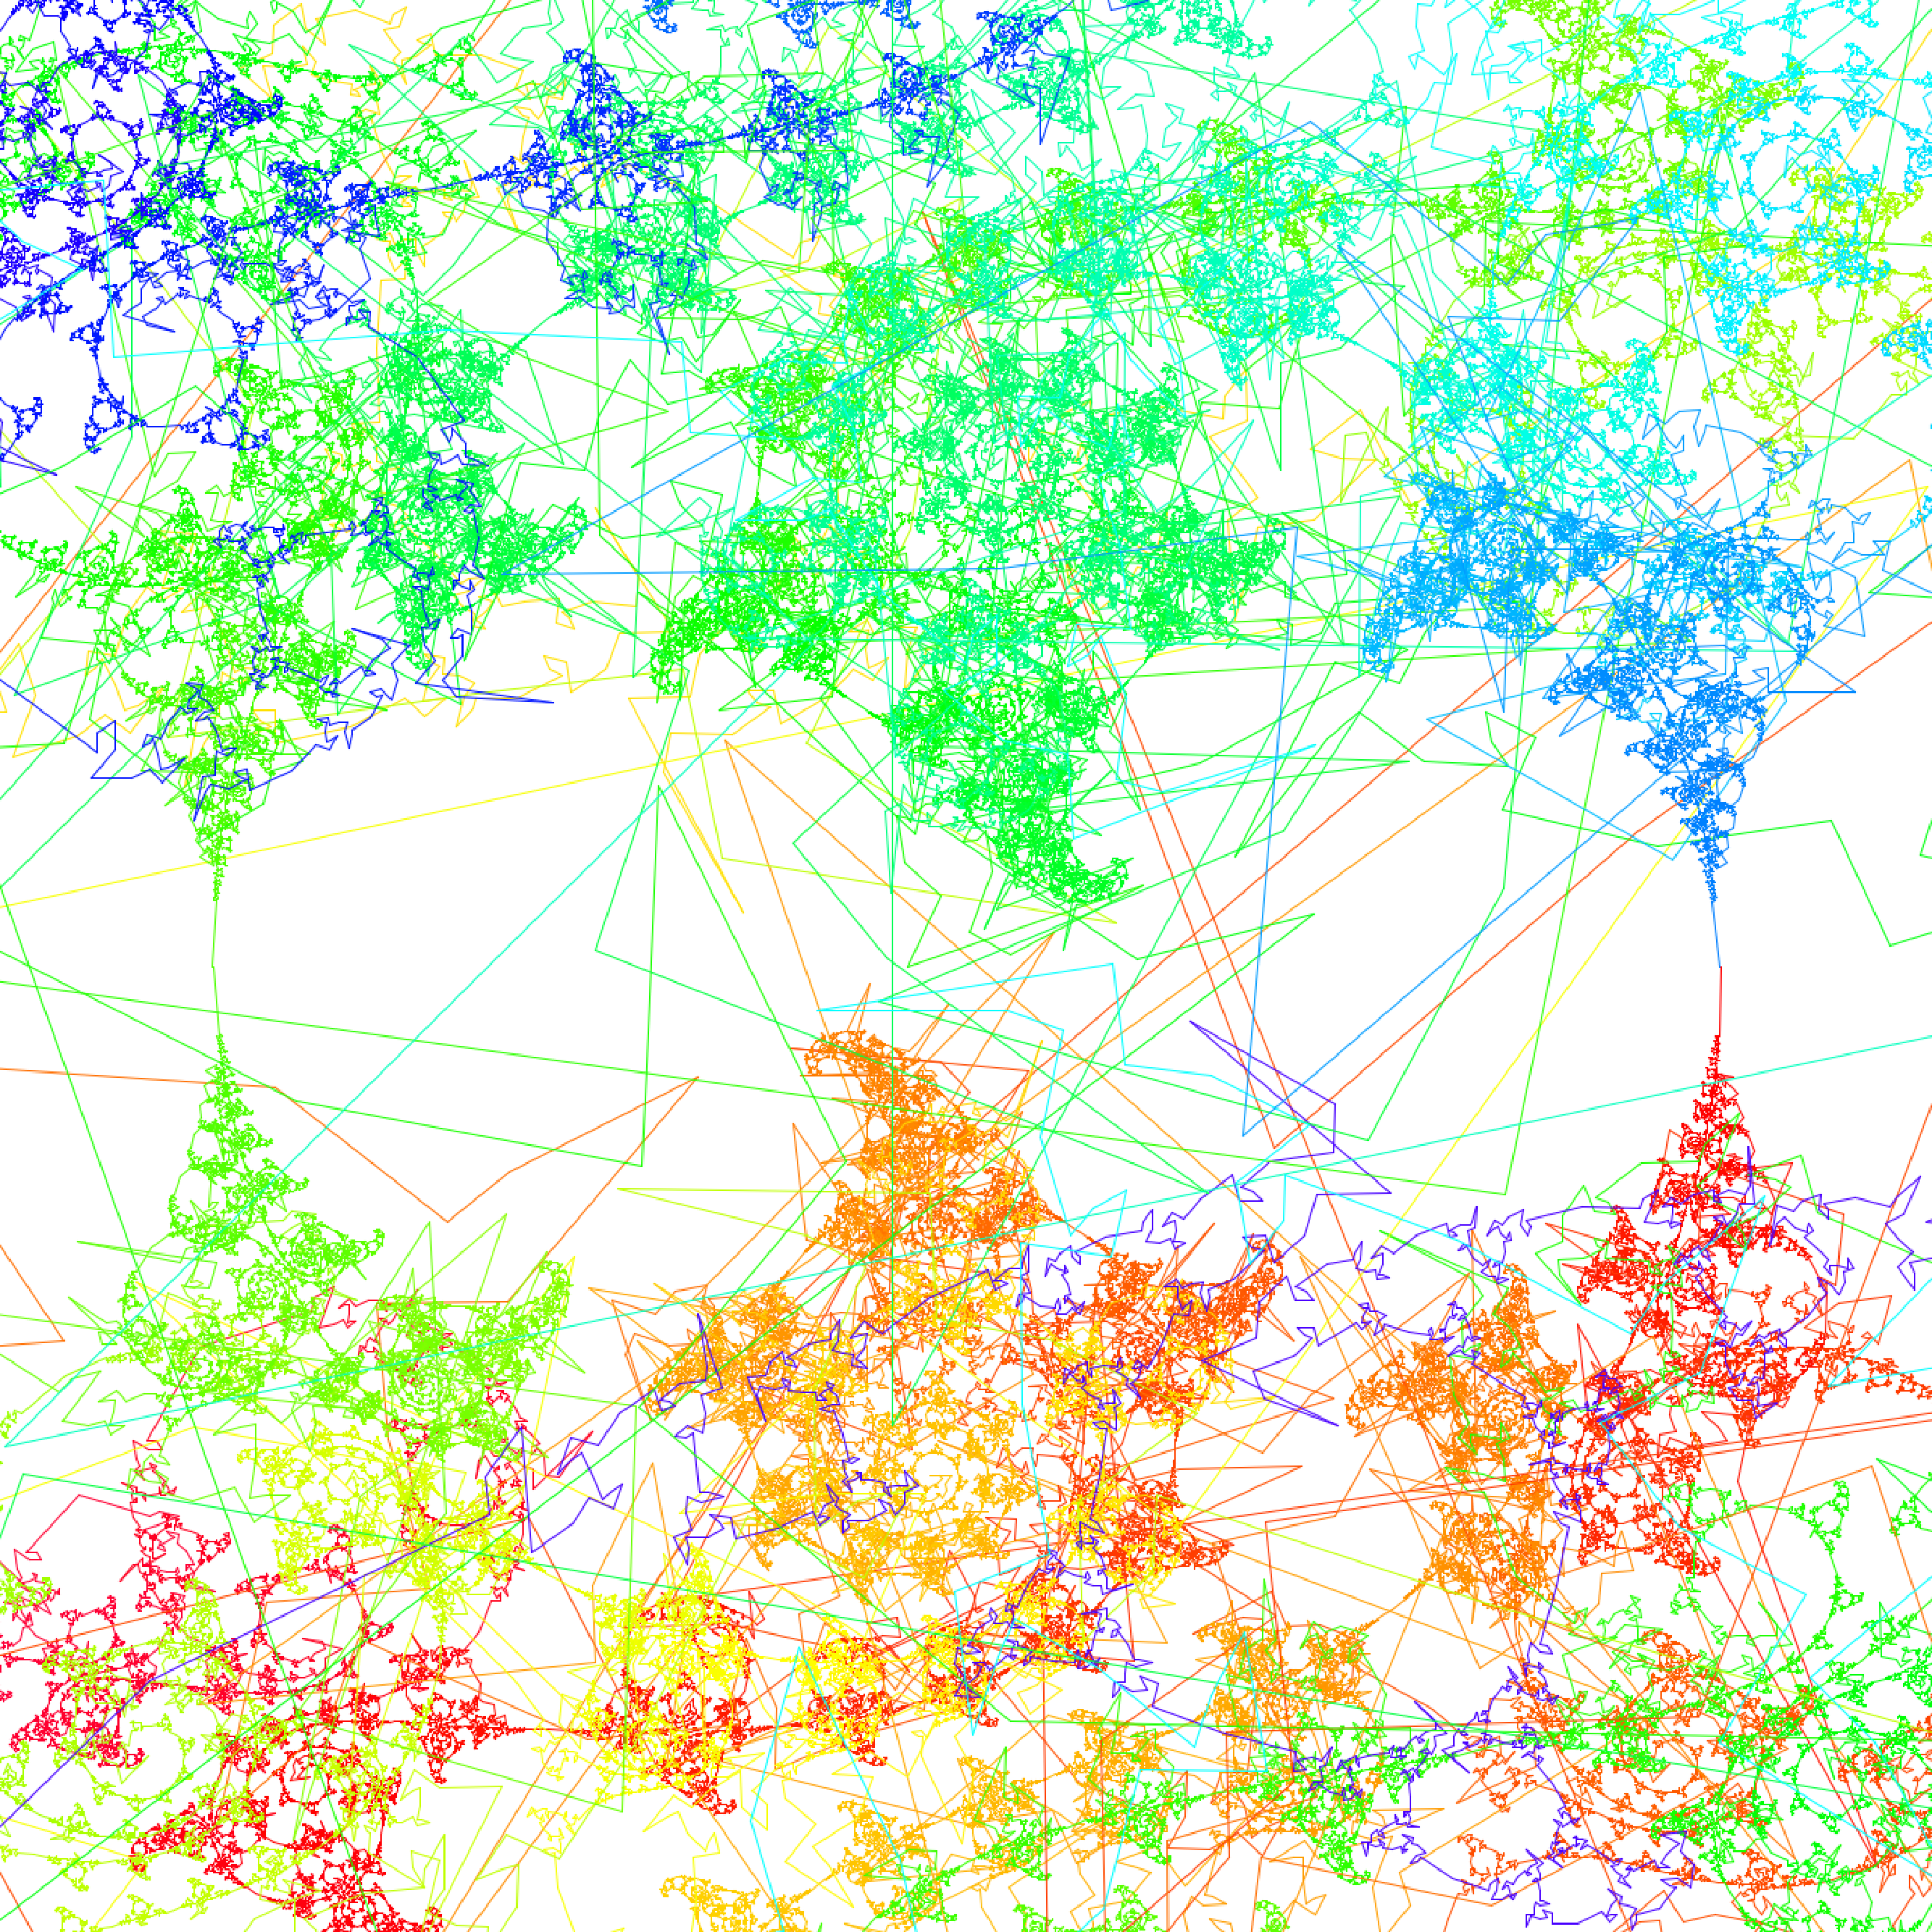
\includegraphics[ height=2.5in, keepaspectratio]{../img/klein/limitset/non-discrete2.pdf}
  \subcaption{}
 \end{minipage}
 \caption{The limit set of non-discrete groups}
 \label{fig:non-discrete}
\end{figure}

\subsubsection{Faults of Graph Traversal Approach}

ケーリーグラフを探索する方法にはいくつかの欠点がある.
まず,生成元の数を増やしたり,探索を深くしたりするごとに指数オーダーで計
算量が増えてしまうことが挙げられる.
さらに,木構造の探索はそもそも並列化に向かないため,高速化が難しい.
また,部分的に図を拡大したい場合に無駄な部分を計算しないといった処
理にも手間がかかる.
このような欠点を避けるため,木構造の探索に頼らない方法がいくつか考案され
ている.

しかしながら,最新のOpenCLやCUDAといった並列計算プラットフォームでは
Dynamic Parallelismという機能を用いることで,木構造探索の並列計算を効率
よく行うことが可能である.
ただし,最新のハードウェアに依存した機能のため,どの計算機環境でも使える
とはいえない.

\subsection{Iterated Inversion System}

ケーリーグラフの探索に依らないアルゴリズムを考案するにあたり,
筆者らは1章でみた,シェーダを用いたフラクタルのレンダリングアルゴリズム
を参考にした.
そして,円や球の反転で構成される群の軌道を高速に描画するためのアル
ゴリズム,\textit{Iterated Inversion System (IIS)}~\cite{bridges2016-367}
を開発した.
円や球の座標と半径を直接計算するこれまでのアプローチに対して,このアルゴ
リズムは任意の点が属する円や球の深さを特定する.
これはスクリーンスペースのピクセルそれぞれに対して独立に計算することがで
きるので,シェーダによる並列計算と描画を行うことができる.

\subsubsection{The Algorithm}

アルゴリズムは非常にシンプルである.
図\ref{fig:iis-orb}のような四つの反転円の軌道を描くことを考える.
ここで,すべての円の外側である黒い領域を\emph{基本領
域}(\textit{fundamental domain})とよぶ.

IISは平面状の全ての点に対して計算を行う.
ある点がいずれかの反転円に属している時にその反転円に関する反転を作用させ
る.
この操作を反転後の点が基本領域に移されるまで繰り返す.
最終的に行なった反転の回数が,その点が属している円盤の深さとなる.
図\ref{fig:iis-orb}では青い点を反転を繰り返して移した軌道を描いている.
この点は2回の反転によって基本領域に到達したので,下から2番目の円に属し
ている.反転の回数に応じて色を変えて点を塗ることで円列が可視化される.

実際に,このアルゴリズムを用いてすべての点を基本領域へと移動させるためには,
無限回の反転が必要である. そのため,あらかじめ最大の反転回数を決めてお
く必要がある.
それぞれの計算は最大の反転回数と反転円の数の多項式時間で描画することができる.
また,画面に入っている部分のみを計算するので,無駄な部分は計算されない.

反転円同士が接触しているとき,極限集合は平面を二つに分割する.
極限集合の内側の点はIISによって内側の基本領域に移され,極限集
合の外側の点は外側の基本領域に移される.
そのため,内側の基本領域に移された点のみを描画することで図
\ref{fig:schottkyEdge}のように極限集合の境界を描くことも可能である.

\begin{figure}[htbp]
 \begin{minipage}{0.5\hsize}
  \center
  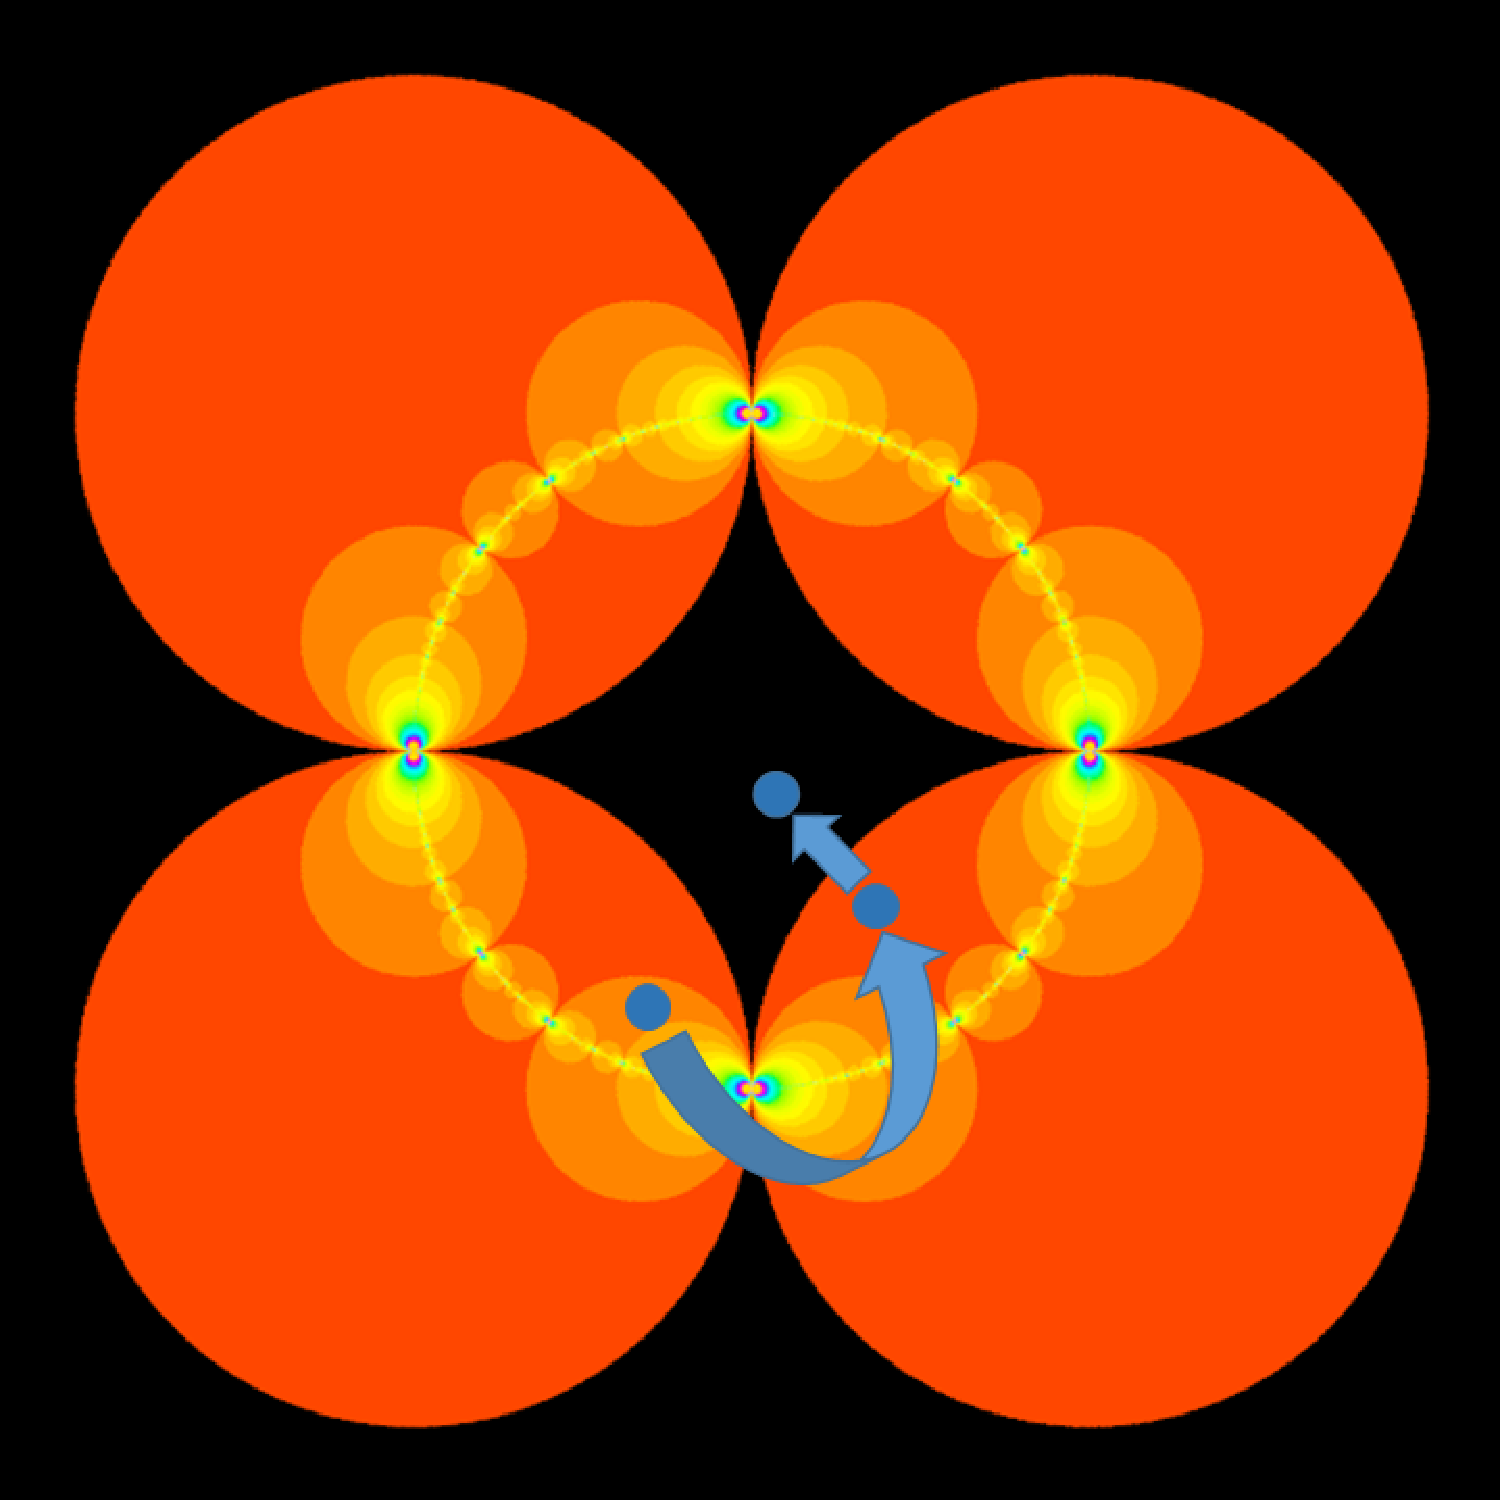
\includegraphics[ height=2.5in, keepaspectratio]{../img/klein/iisOrb.pdf}
  \caption{The process of IIS}
  \label{fig:iis-orb} 
 \end{minipage}
 \begin{minipage}{0.5\hsize}
  \center
  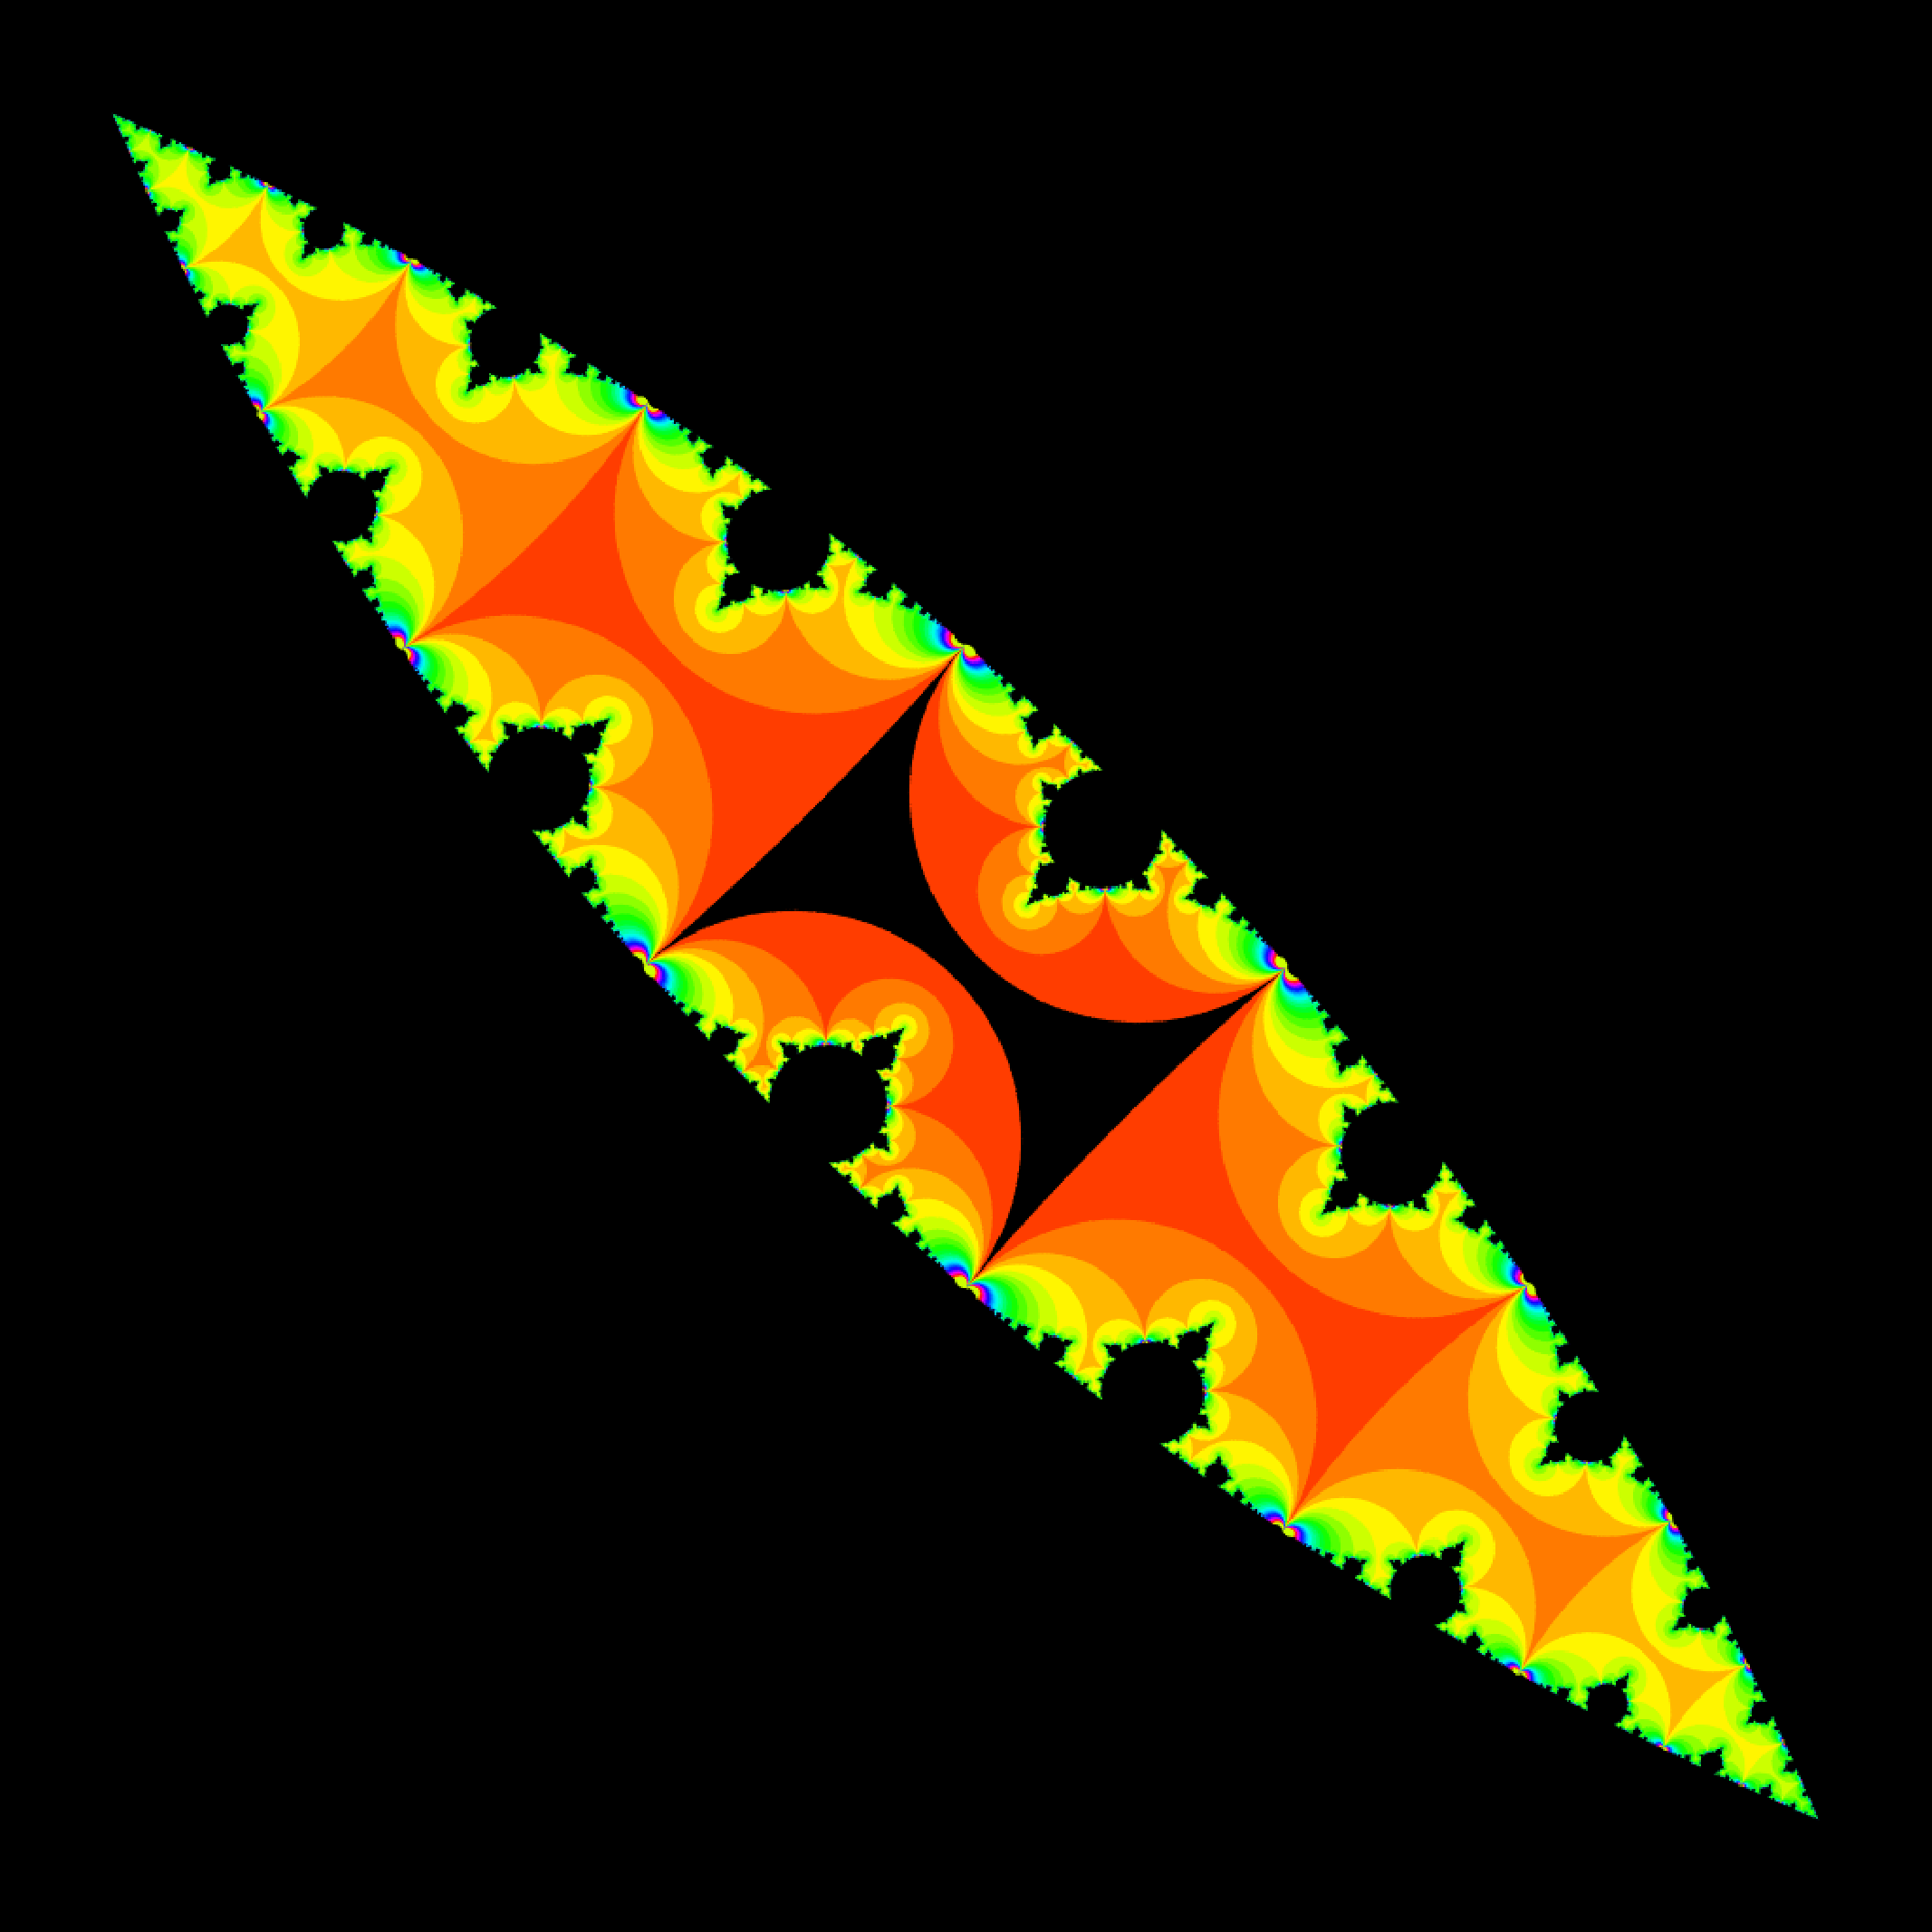
\includegraphics[ height=2.5in, keepaspectratio]{../img/klein/schottkyEdgeRect.pdf}
  \caption{The edge of the limit set}
  \label{fig:schottkyEdge}
 \end{minipage}
\end{figure}

IISの擬似コードをアルゴリズム\ref{alg:iis2d}に示す.
後に,我々は単純な円の反転以外の生成元を導入する.
そのため,基本領域上にある点に対しては恒等変換を,その他の点に対しては反
転,もしくは反転の合成を作用させる写像$G$を用いて,これを記述した.

 \begin{algorithm}
  \caption{Iterated Inversion System (IIS)}
  \label{alg:iis2d}
  \begin{algorithmic}
   \REQUIRE count $= 0$ and coordinates $=$ position determined by
   pixel
   \FOR{$i=0$ to \texttt{MAX\char`_INVERSION}}
   \STATE inFundamentalDomain $\leftarrow$ \TRUE
   \FOR{ each map $G$ in Maps }
   \IF{$G$ is available to coordinates}
   \STATE coordinates $\leftarrow$ $G(\text{coordinates})$
   \STATE INCREMENT count
   \STATE inFundamentalDomain $\leftarrow$ \FALSE
   \ENDIF
   \ENDFOR
   \IF {inFundamentalDomain}
   \STATE BREAK for
   \ENDIF
   \ENDFOR
   \STATE RETURN count
  \end{algorithmic}
 \end{algorithm}

\subsubsection{3D Extension}

このアルゴリズムは三次元空間における球の反転に対しても用いることができる.
空間上の点に対しても点が属している球の深さを計算することができるが,球に
よる反転の軌道は球の内側に入り込むため,二次元の場合と同様に描画するには
手間がかかる.
そこで我々は軌道の元となる球を用意し,その球を球の反転の組み合わせで
移した軌道を描画する.
図\ref{fig:3baseSphereGen}に描かれている三つの緑の球をすべての灰色の球の
反転の組み合わせで移した軌道が図\ref{fig:3baseSphereOrb}のようになる.
ここで,図\ref{fig:3baseSphereGen}における灰色の球を\emph{反転球},緑色
の球を\emph{基本球}とよぶ.

\begin{figure}[htbp]
 \begin{minipage}{0.5\hsize}
  \center
  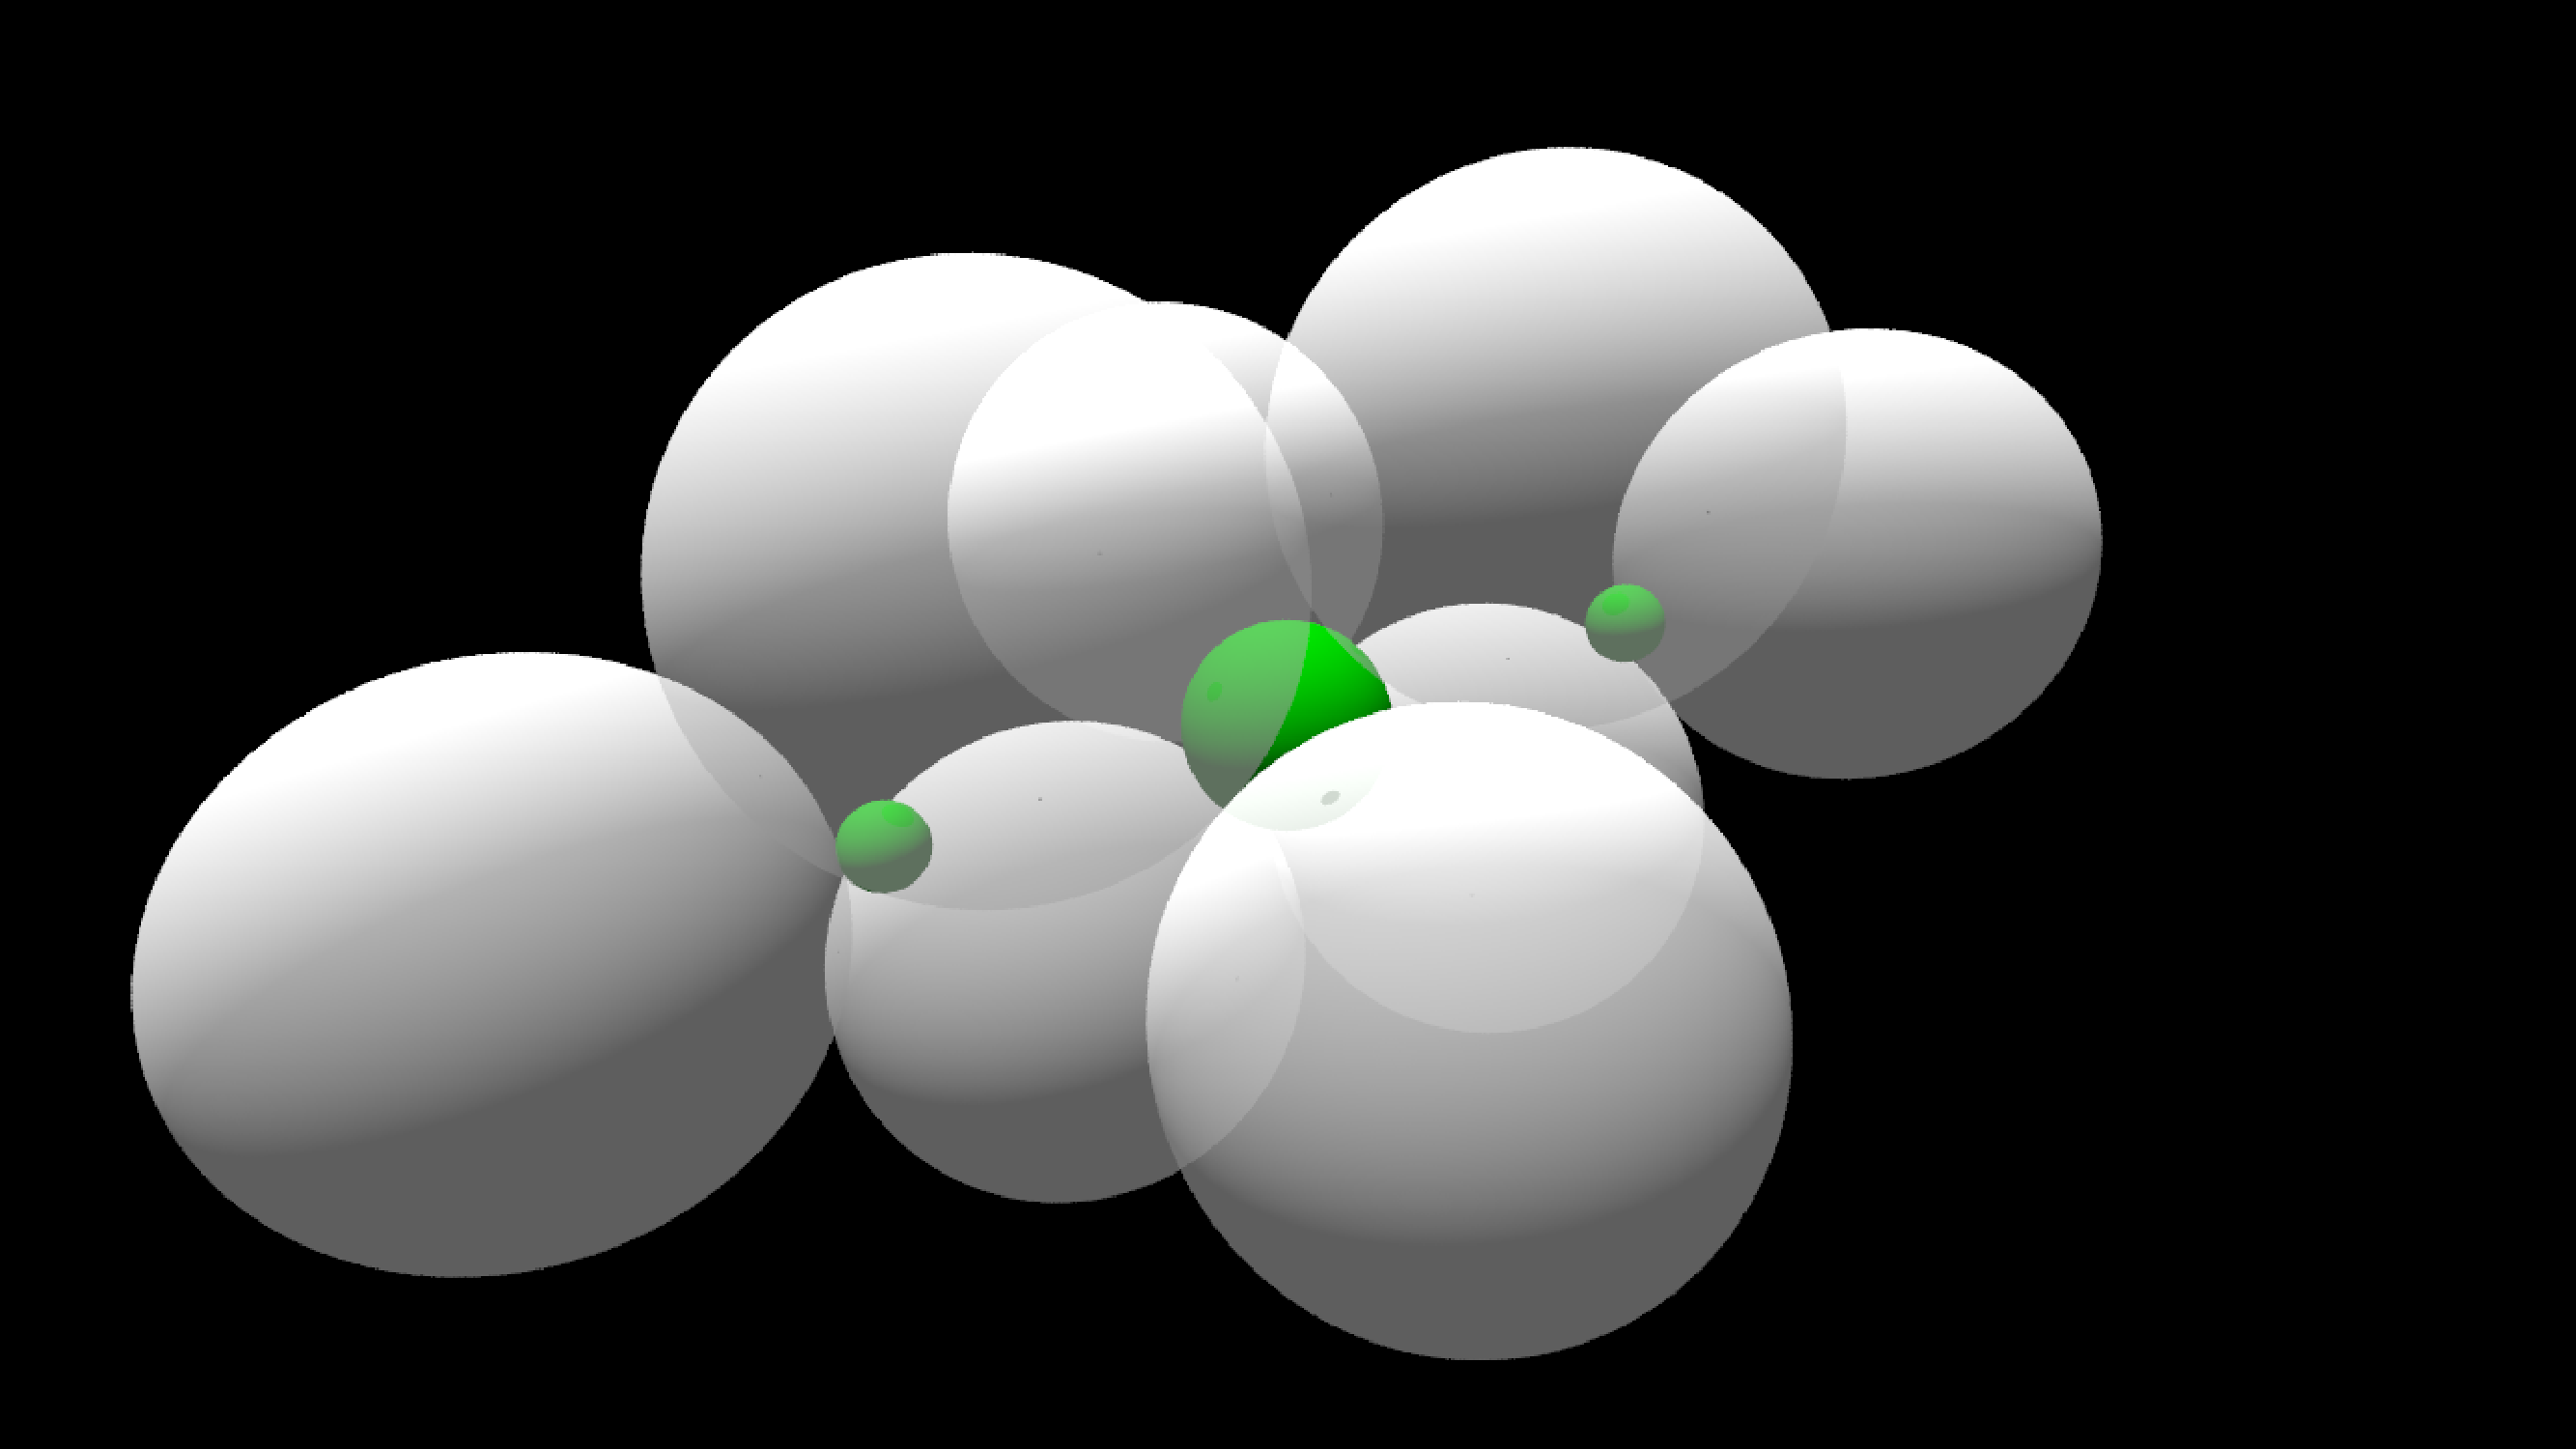
\includegraphics[ height=1.7in, keepaspectratio]{../img/klein/3baseGen.pdf}
  \subcaption{Generator}
  \label{fig:3baseSphereGen}
 \end{minipage}
 \begin{minipage}{0.5\hsize}
  \center
  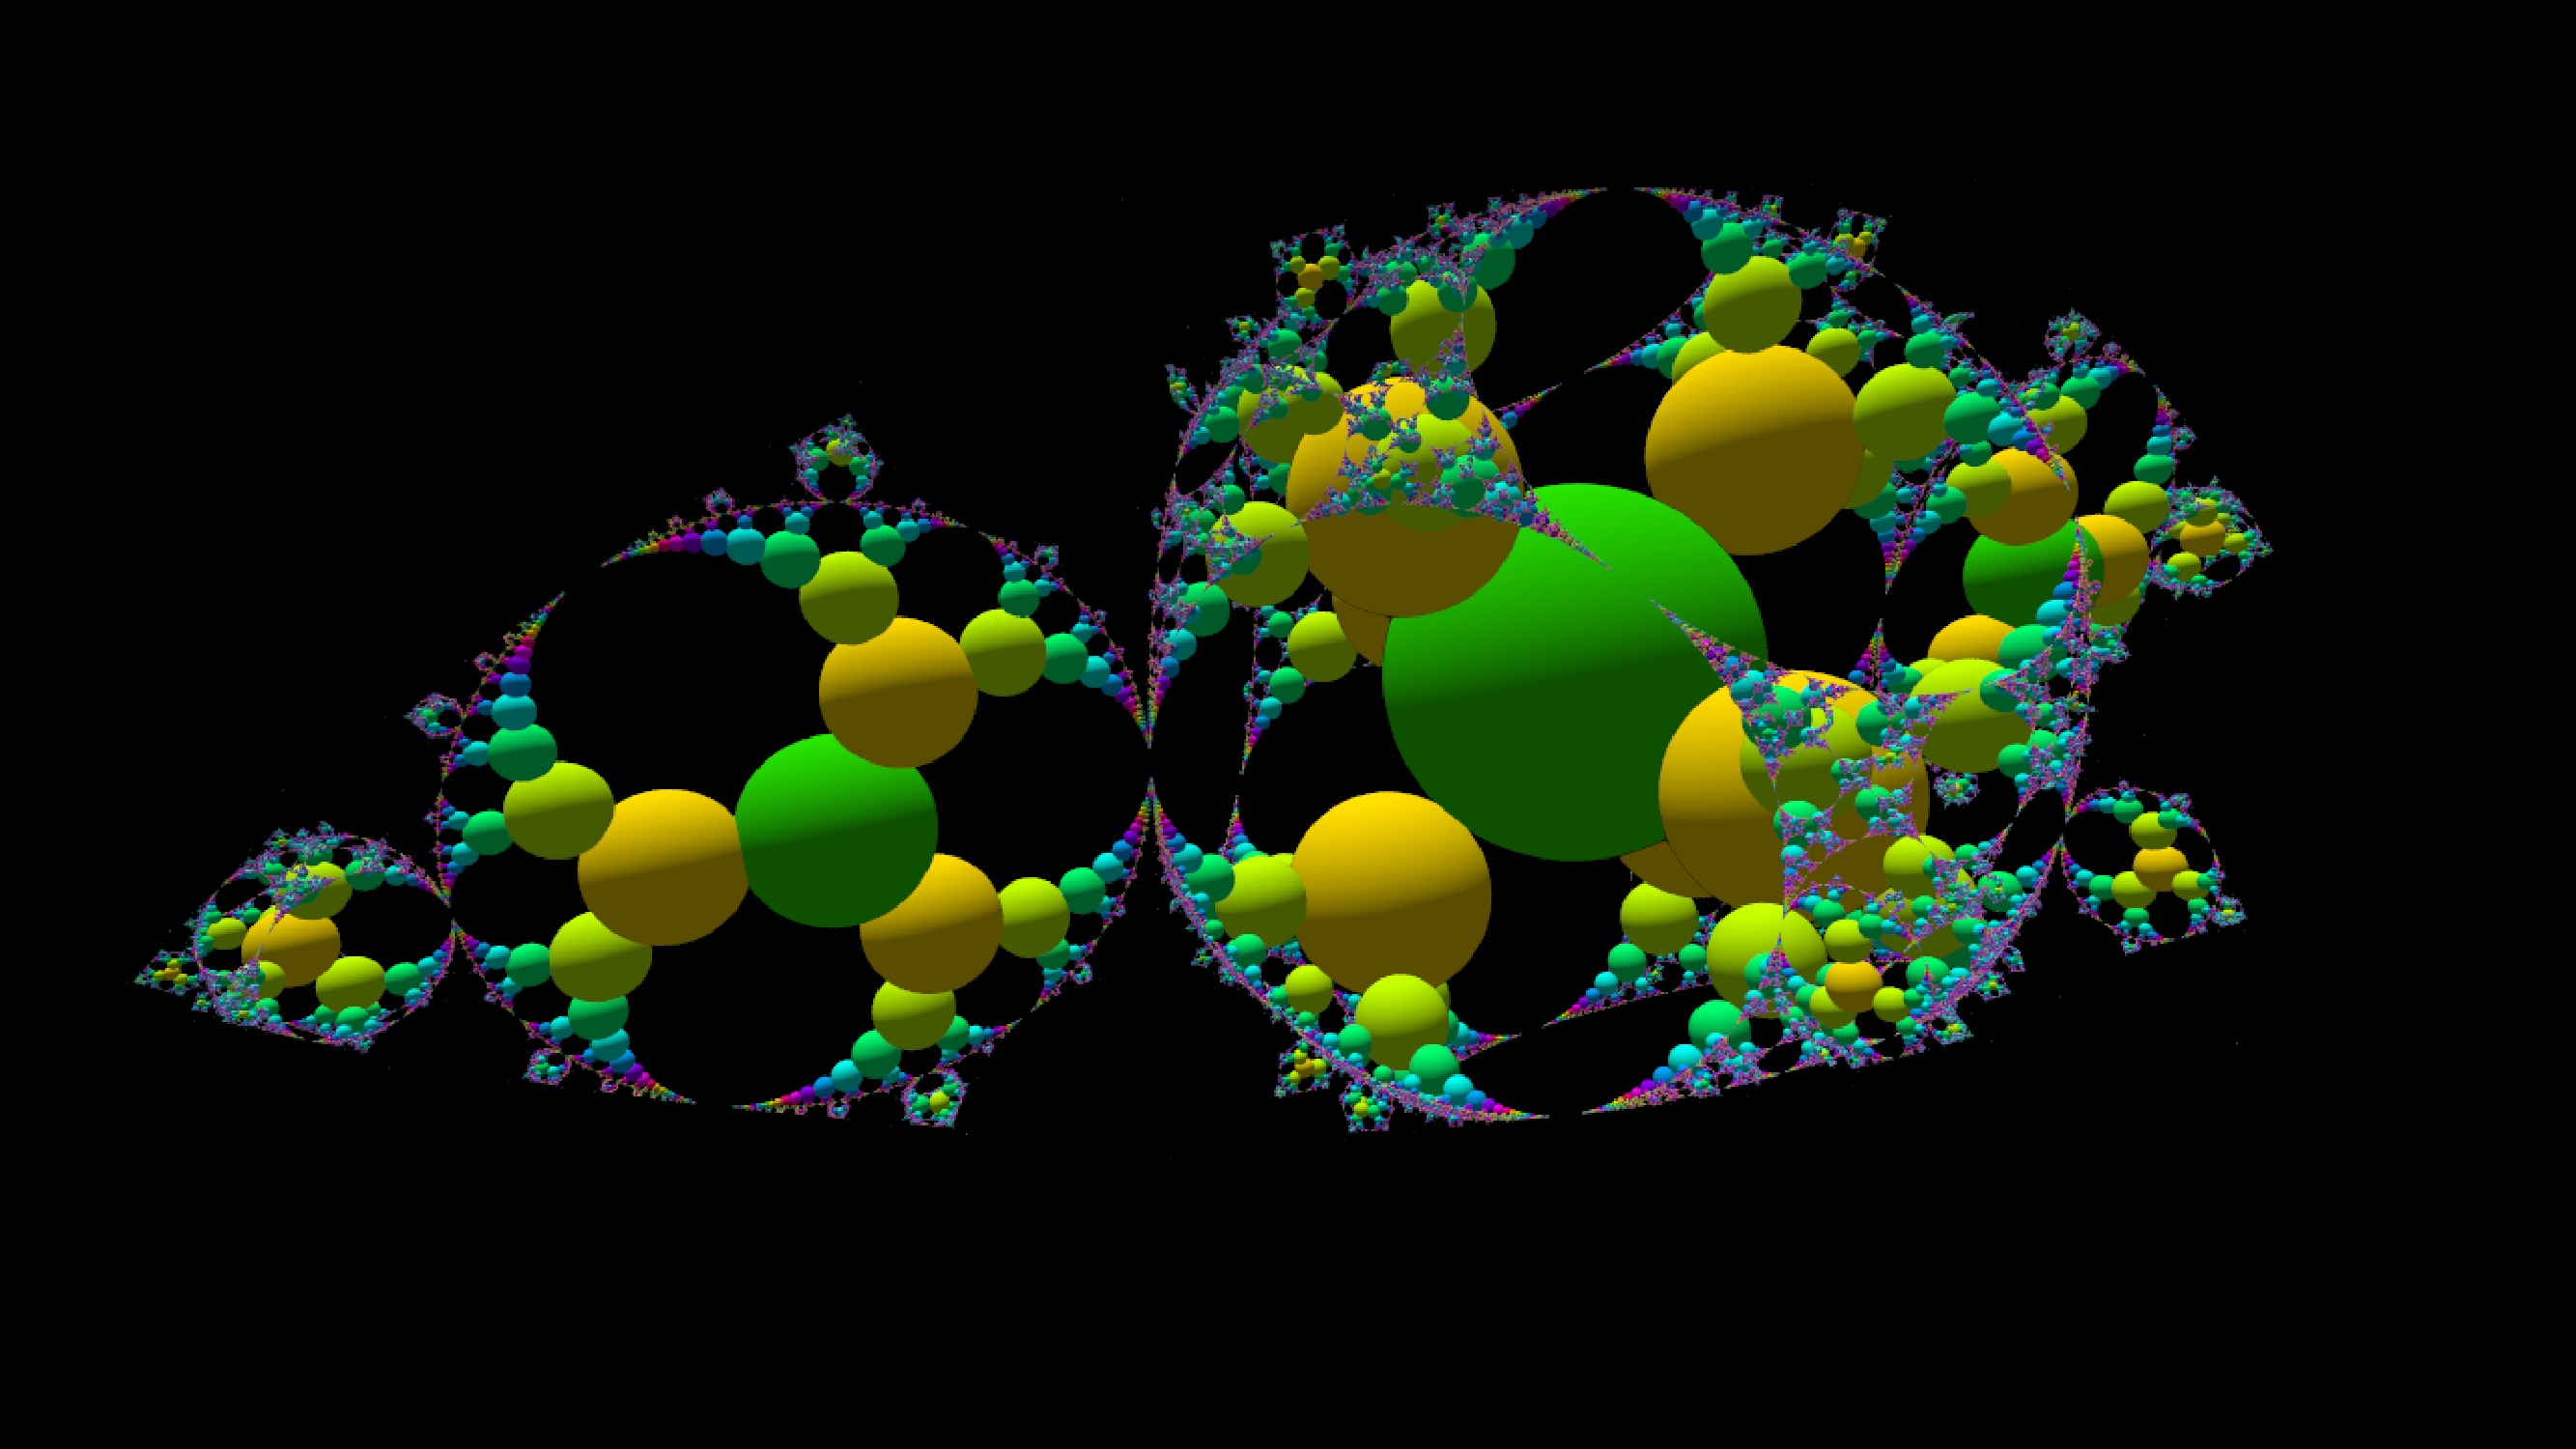
\includegraphics[ height=1.7in, keepaspectratio]{../img/klein/3baseOrb.pdf}
  \subcaption{Orbit}
  \label{fig:3baseSphereOrb}
 \end{minipage}
 \caption{The orbit of 3 base spheres}
 \label{fig:3baseSphere}
\end{figure}

これはレイマーチングとDistance Estimationを用いることで高速に描画するこ
とができる.レイマーチングに用いる距離関数を導出するため,ここから図
\ref{fig:simple3diis}に示されるような六つの反転球と一つの基本球による
軌道を考える.
簡単のために,この図のXY平面での断面を図\ref{fig:xySlice}に示した.
反転球の軌道の断面は図\ref{fig:levelMax}と同様の円列となる.
また,基本球の軌道の断面は\ref{fig:simpleOrb3d}と同様の色をつけた.
白の点$P2$はレイの先端であり,これに最も近い球は$S2$である.
白の点$P1$は$P2$の属する反転球で$P2$を反転した像である.
また,$S1$は$S2$をそれが属する反転球で移した像であり,基本球でもある.
距離関数は$P2$から$S2$までの距離を返す必要がある.
しかし,$S2$の位置と半径は分からない.
そこで,我々は球の反転のヤコビアンを用いて,点$P1$と基本球である$S1$から求
める距離を逆算する.
求める距離を$d$,$S1$の半径と中心をそれぞれ$S1r,~S1c$とすると,$d$は次の
式で近似することができる.
\begin{align*}
 d \approx \frac{distance(P1,~S1c) - S1r}{Jacobian}
\end{align*}
これは1章でみたDistance Estimationと同様のアプローチである.
ここで,反転球の中心を$S$,その半径を$R$,反転を作用させる前の点を$P$と
おくと,球の反転のヤコビアンは次のように計算できる.
\begin{align*}
 Jacobian = \frac{R^2}{distance(P,~S)^2}
\end{align*}
また,半径が無限大の球の反転のヤコビアンは1であることに注意する.

実際の距離関数ではレイの先端にIISを作用させる過程で,球の反転を行う毎にそ
のヤコビアンをかけ合わせていく.
最終的に,基本領域上に移された点から基本球への距離を,ヤコビアンの積で割ること
で近似された距離を求めることができる.
ただし,球から点が離れすぎてしまうと誤差が大きくなってしまうことに注意が
必要である.

また,もう一つ考慮すべき事がある.
レイの先端が図\ref{fig:xySlice}における極限集合より外側にあるとき,その
点は球の反転によって反転球の外側に移されてしまう.
そのため距離関数は実際の最短距離よりも大きな距離を返してしまい,
レイはオブジェクトを突きぬけてしまう.
このことは,図\ref{fig:artifact}に描かれるような乱れを生み出す.
軌道の前面が正しくレンダリングされていないことがわかる.
この不具合を避けるため,算出された距離に定数をかけて縮小する方法をとる.
レイマーチングのステップ数は増えてしまうが,正しく描画することができる.
距離の縮小率は球の大きさによって実験的に決める.

この描画方法では基本球の大きさを反転球と重なりあうように大きくすることで,
反転球の軌道の形状を変形することができる.
図\ref{fig:limitSetOnSphere}は基本球の半径を球面が極限集合と被るような大
きさにしたときのものである.
球の上に極限集合をみることができる.
図\ref{fig:limitObj}はそこから基本球の大きさをさらに大きくした図である.
その形状に数学的な意味はないが,興味深い形になる.

ここでみた距離関数を一般化した擬似コードをアルゴリズム
\ref{alg:iis3d}に示した.

\begin{figure}[htbp]
  \begin{minipage}[]{0.49\hsize}
   \center
   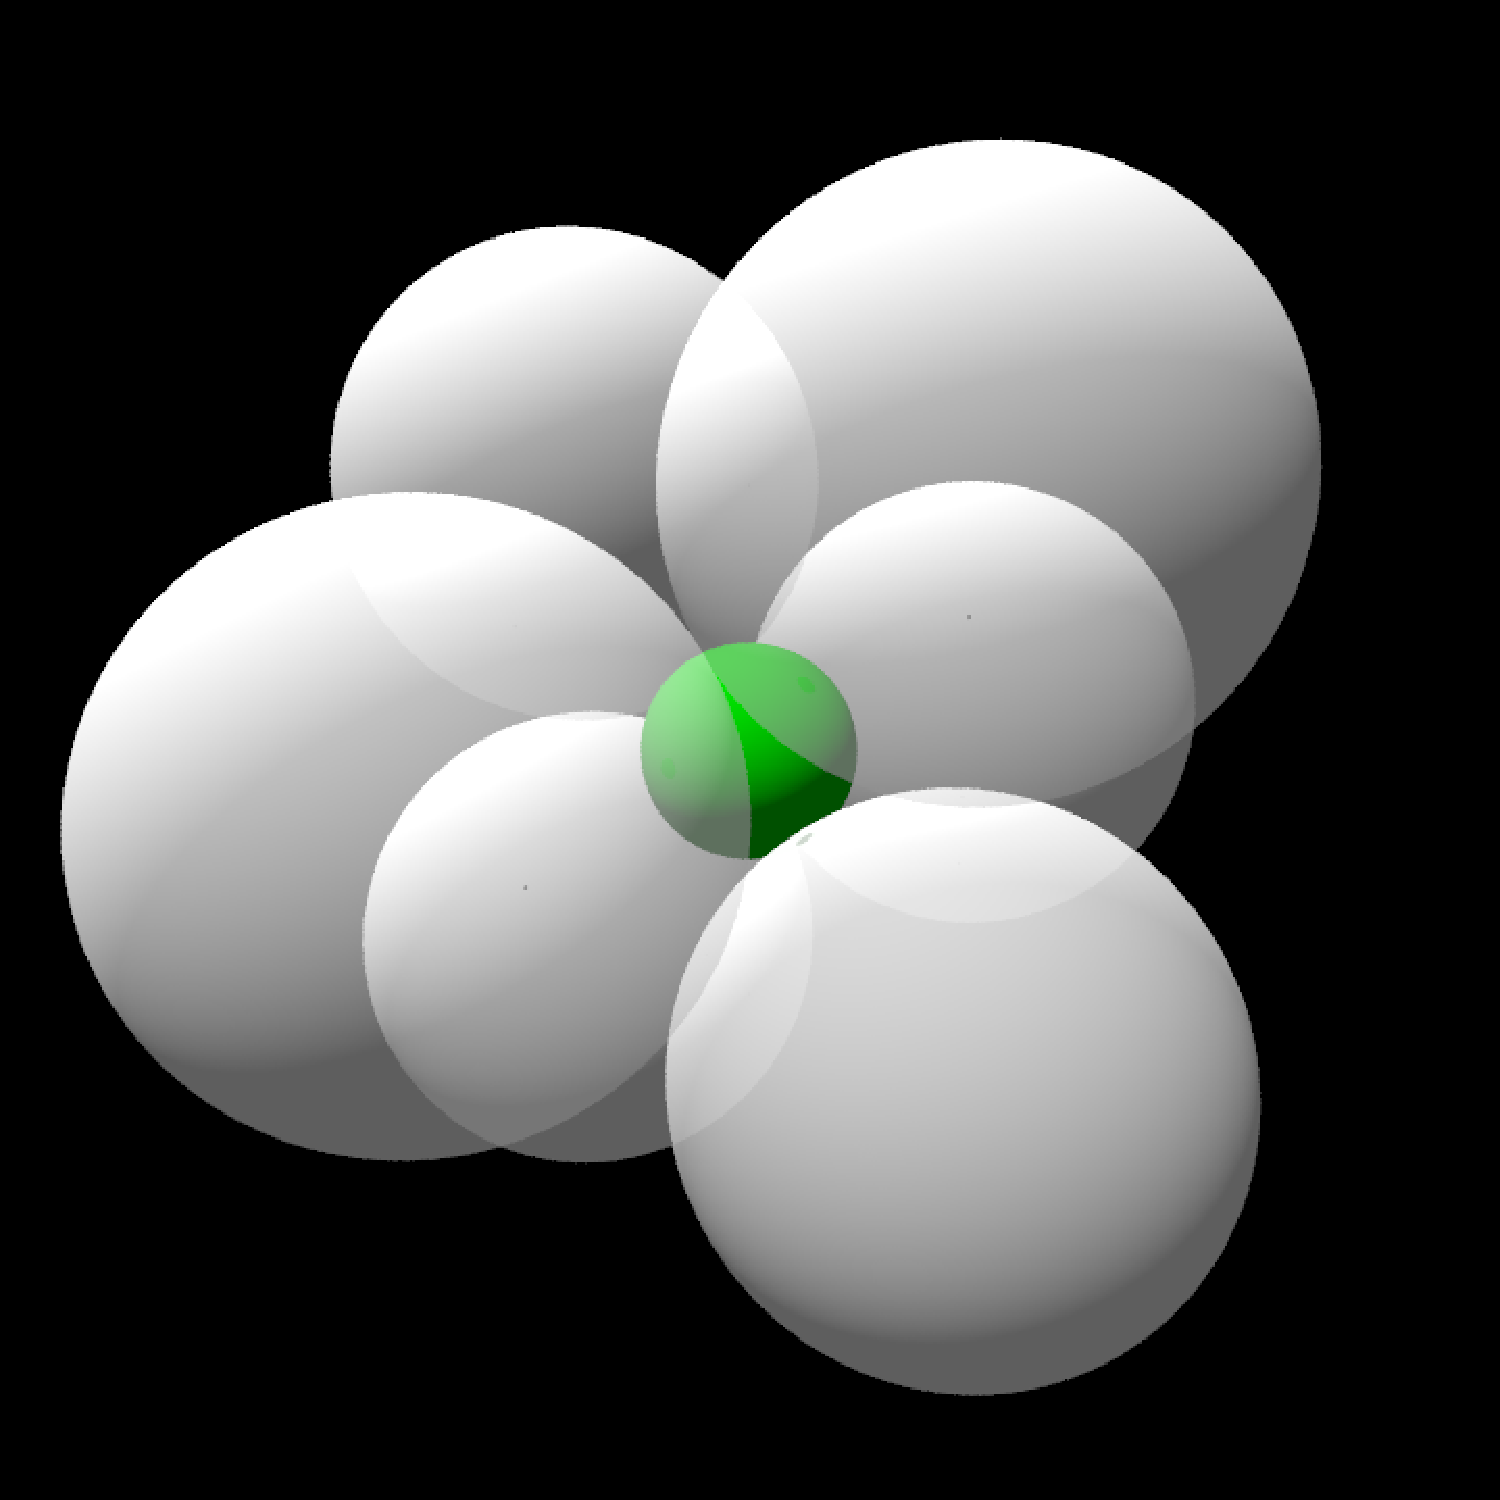
\includegraphics[ height=2.5in, keepaspectratio]{../img/klein/simpleGen.pdf}
   \subcaption{Generator}
   \label{fig:simpleGen3d}
  \end{minipage}
  \begin{minipage}[]{0.49\hsize}
   \center
   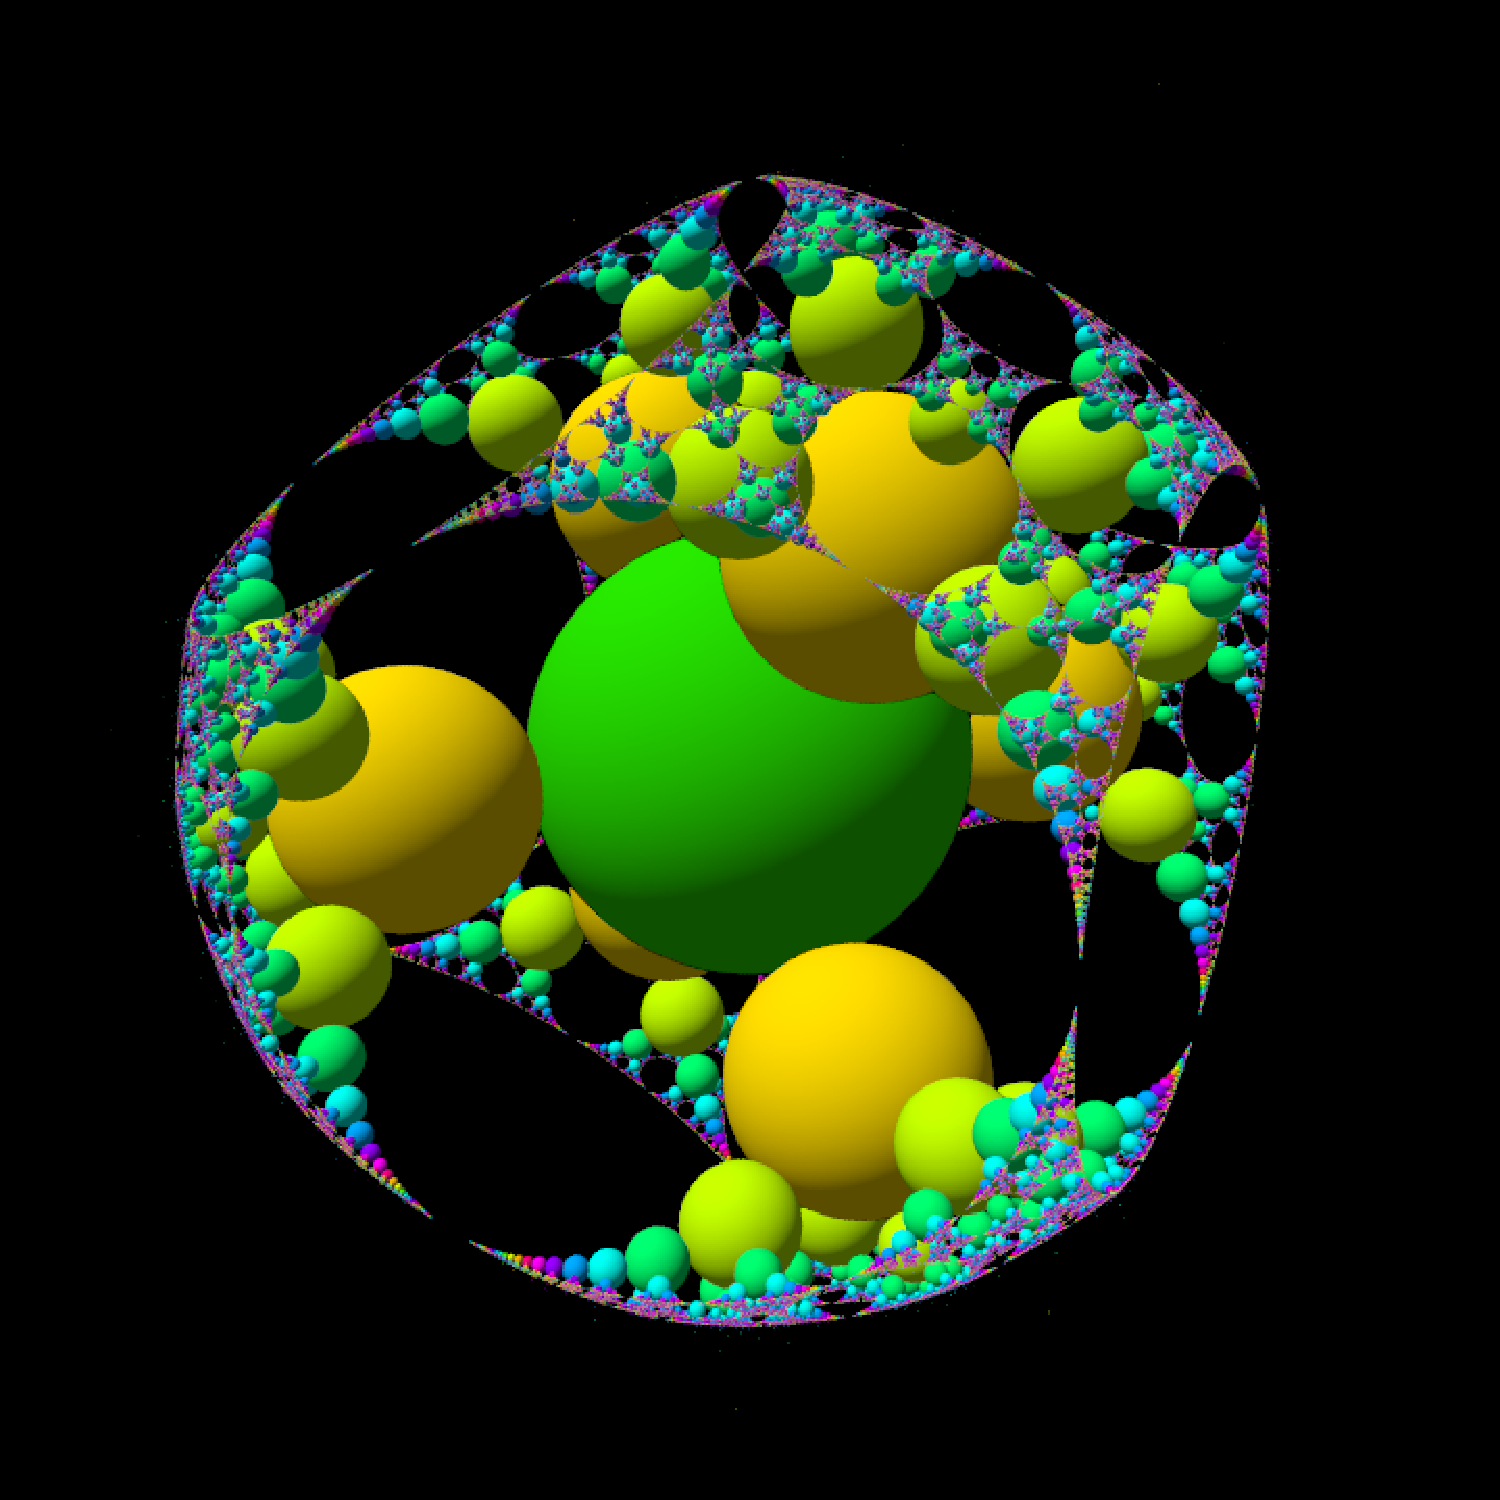
\includegraphics[ height=2.5in, keepaspectratio]{../img/klein/simpleOrbit.pdf}
   \subcaption{Orbit}
   \label{fig:simpleOrb3d}
  \end{minipage}
  \caption{The orbit of the green sphere}
  \label{fig:simple3diis}
\end{figure}

\begin{figure}[htbp]
 \begin{minipage}{0.5\hsize}
  \center
  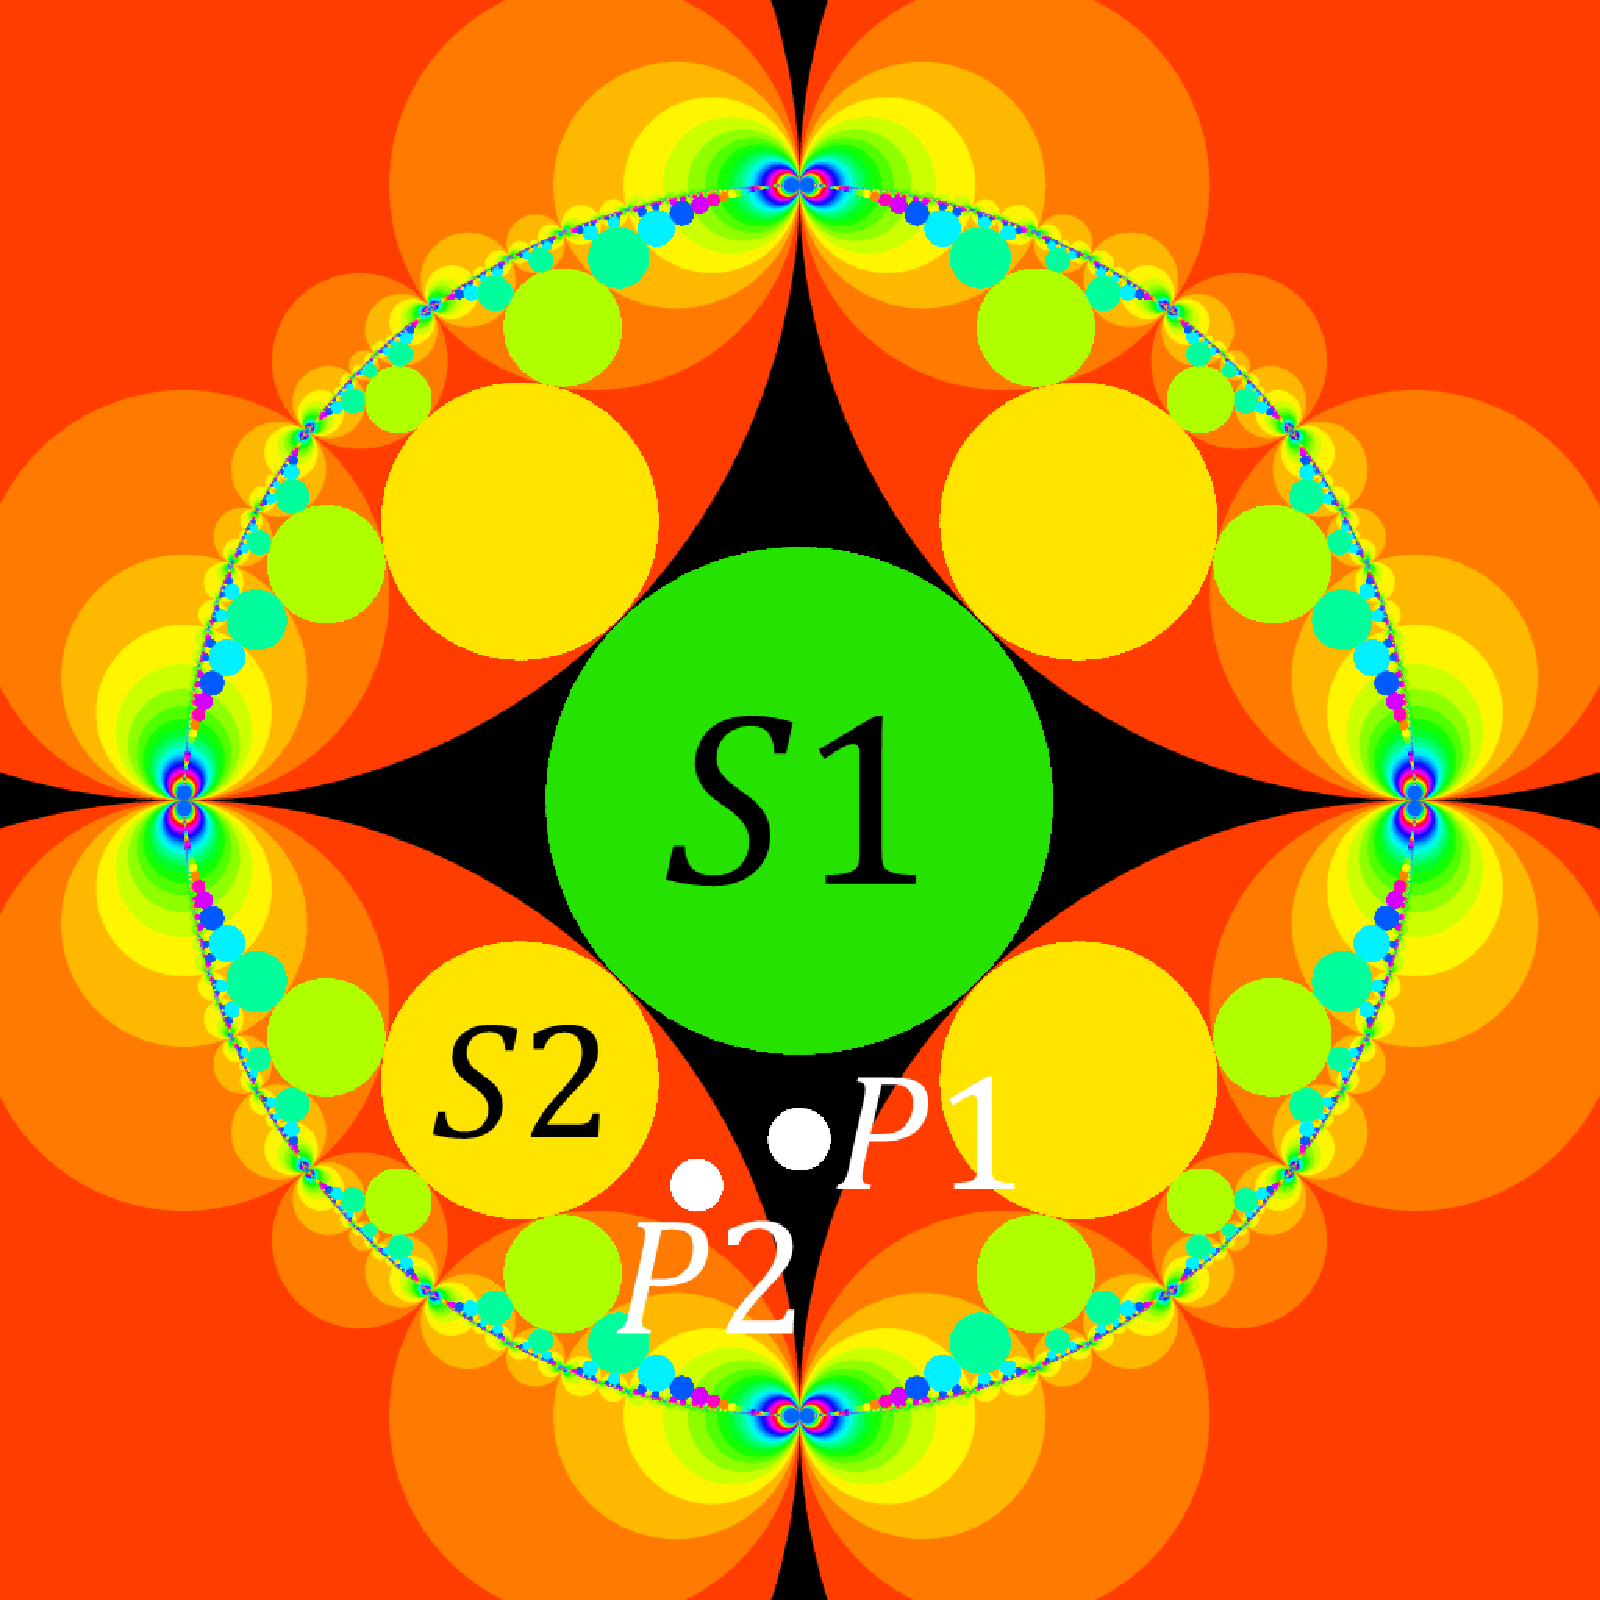
\includegraphics[ width=2.5in, keepaspectratio]{../img/klein/sliceRect.pdf}
  \caption{XY-slice image of Figure \ref{fig:simple3diis}}
  \label{fig:xySlice}
 \end{minipage}
 \begin{minipage}{0.5\hsize}
  \center
  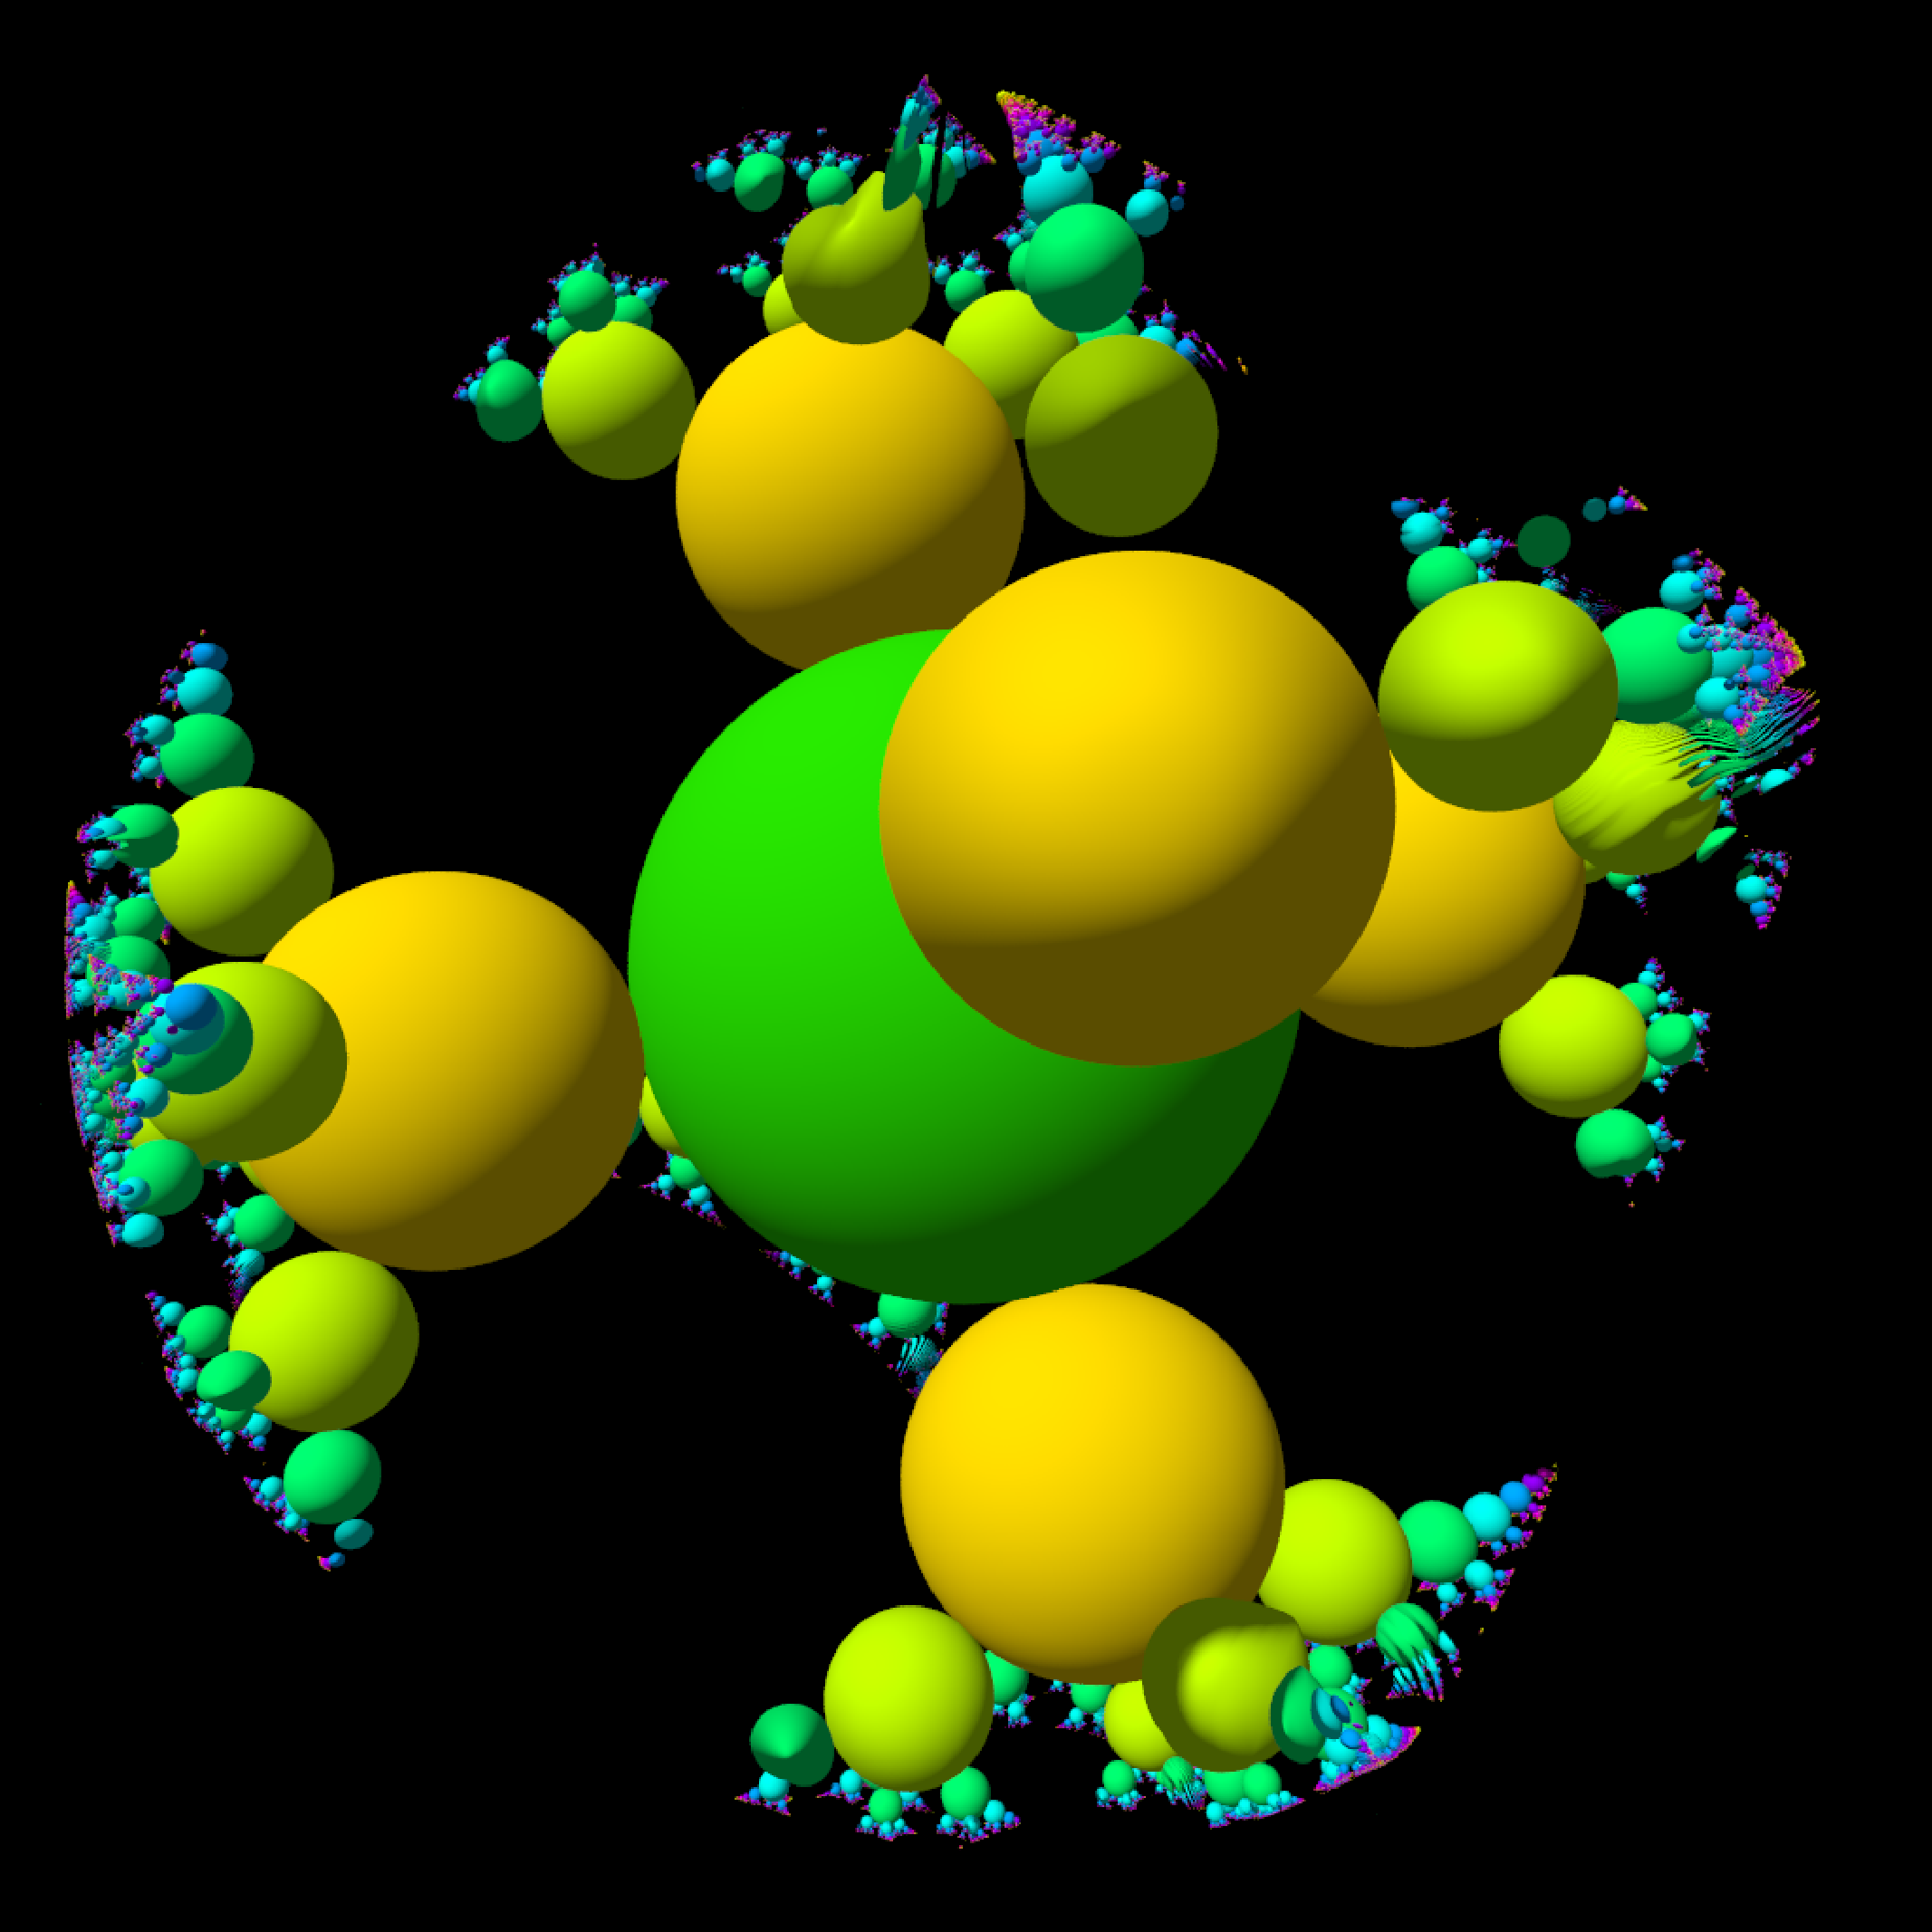
\includegraphics[ width=2.5in, keepaspectratio]{../img/klein/artifactRect.pdf}
  \caption{The Artifact}
  \label{fig:artifact}
 \end{minipage}
\end{figure}

\begin{figure}[htbp]
 \begin{minipage}{0.5\hsize}
  \begin{minipage}{0.24\hsize}
   \center
   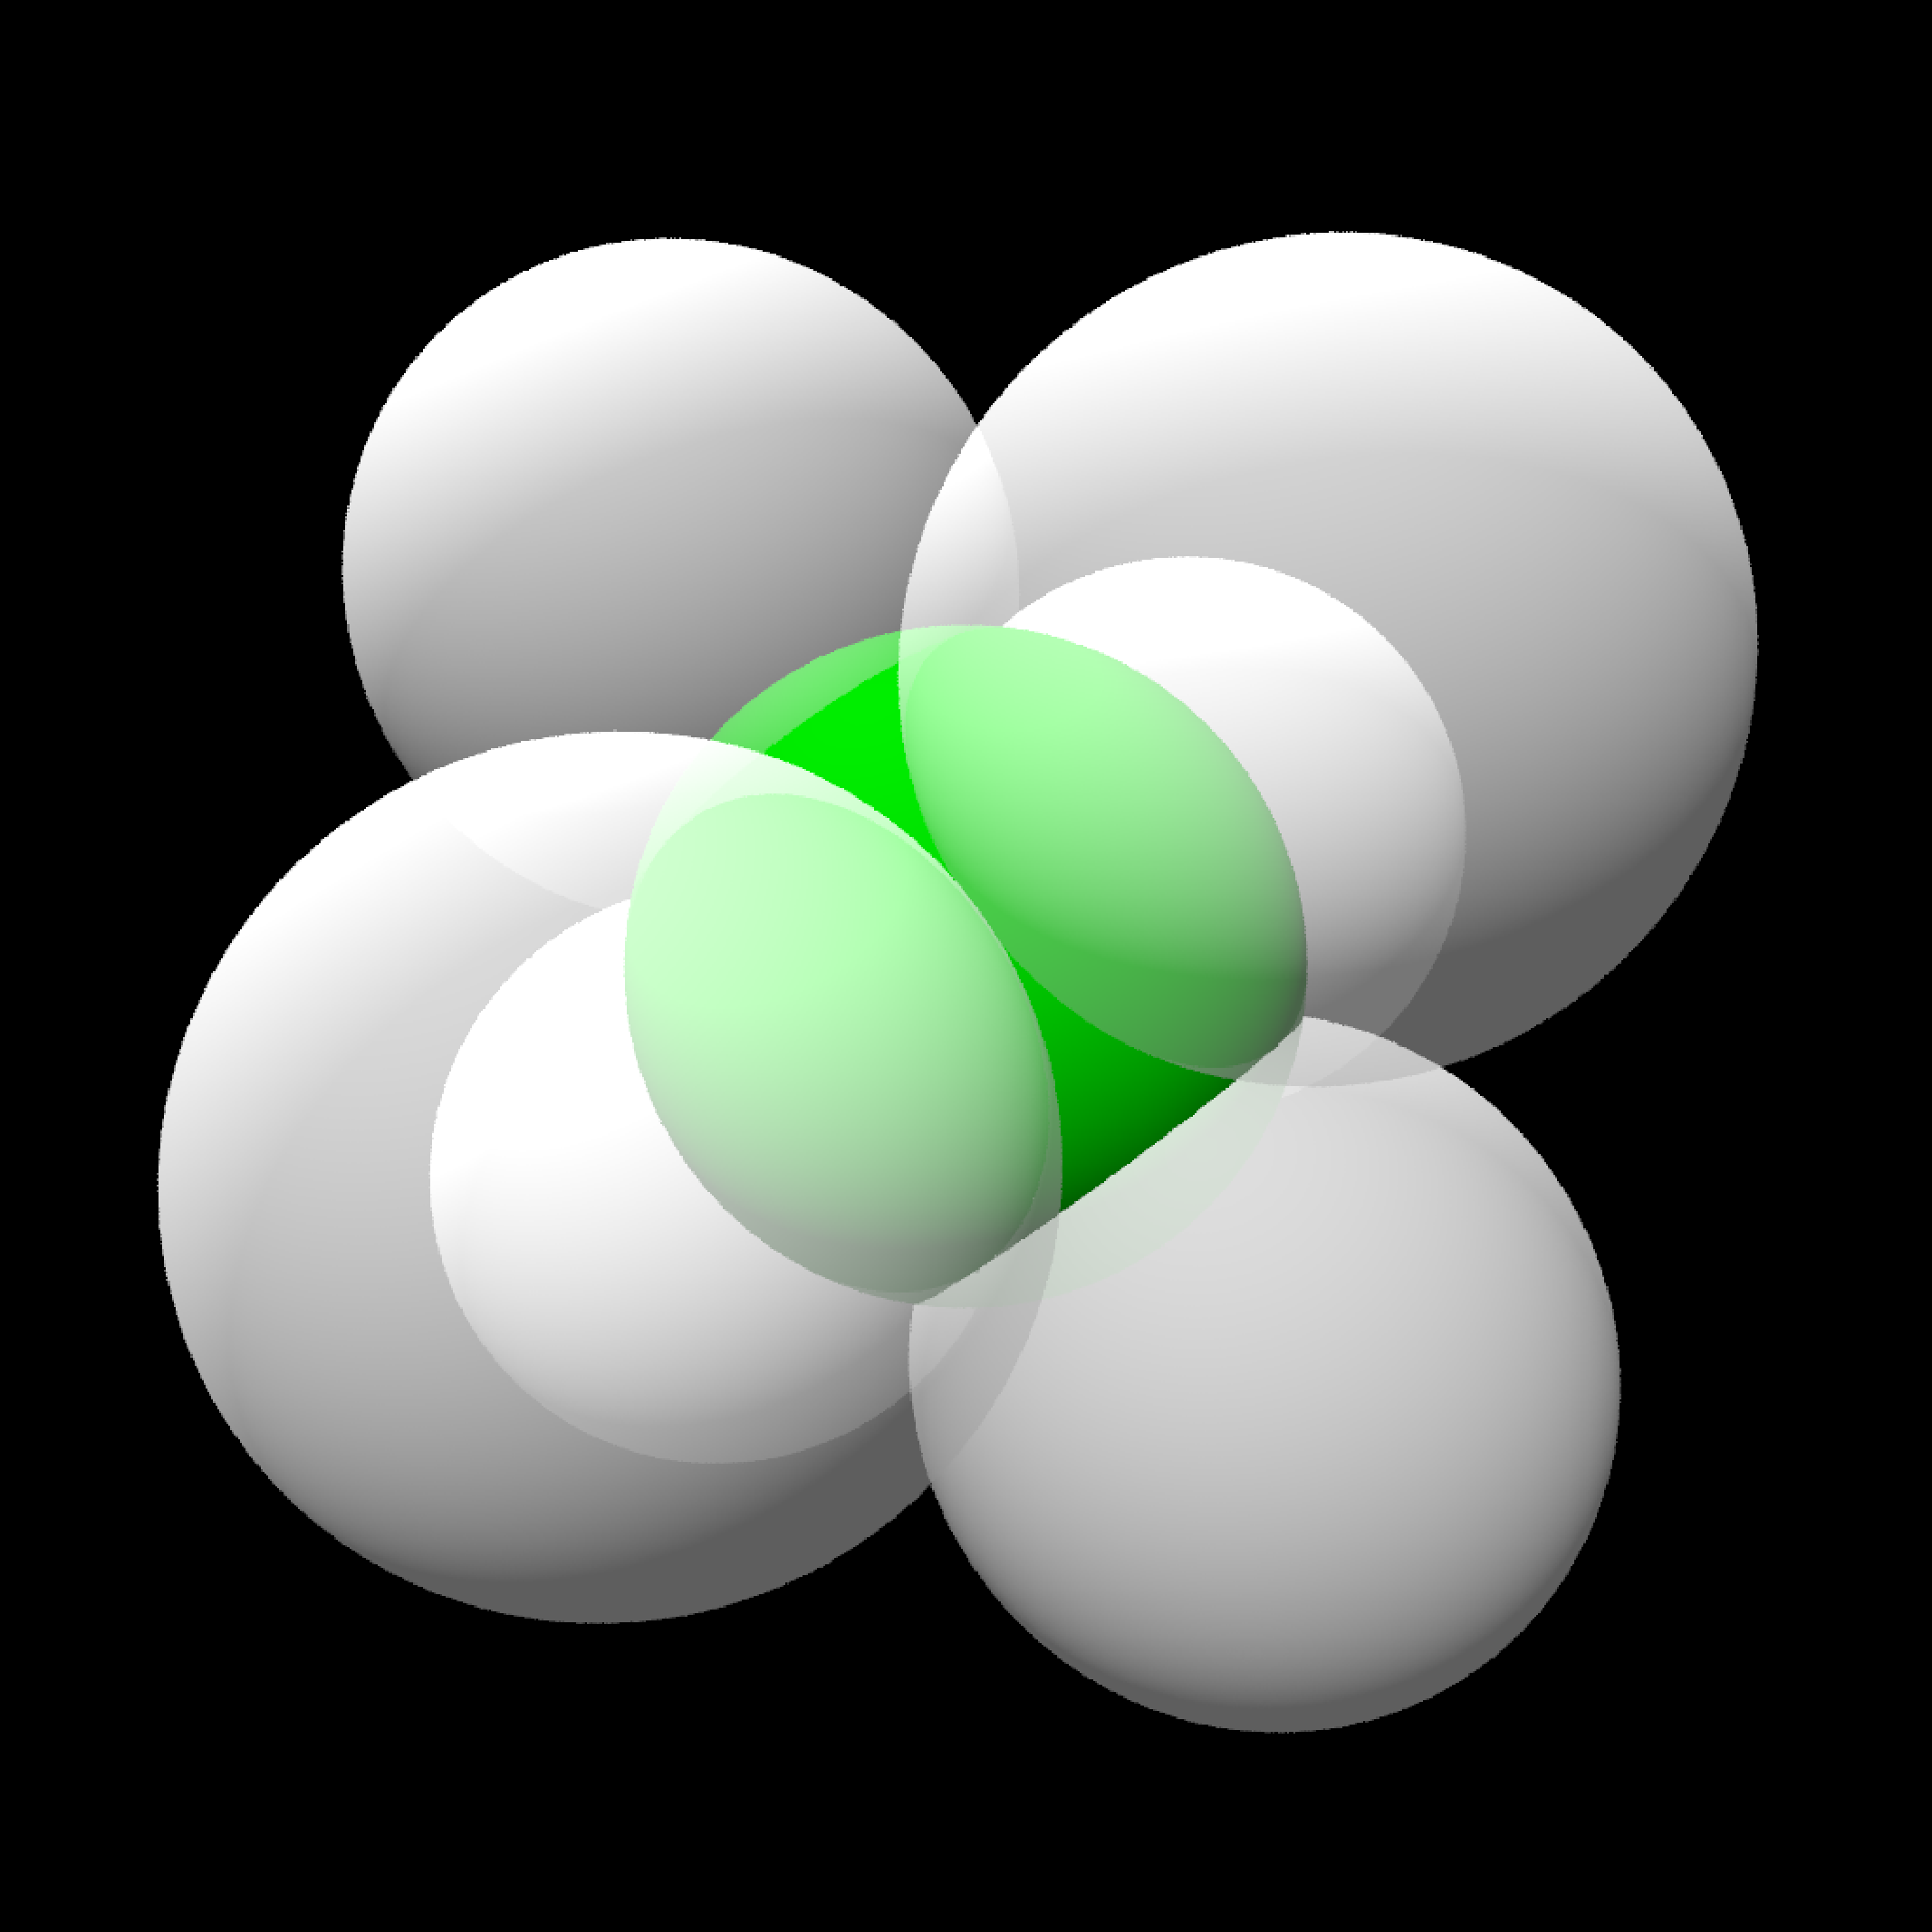
\includegraphics[ height=1.5in, keepaspectratio]{../img/klein/limitSetOnSphereGen.pdf}
   \subcaption{Generator}
  \end{minipage}
 \hspace*{\fill}
  \begin{minipage}{0.24\hsize}
   \center
   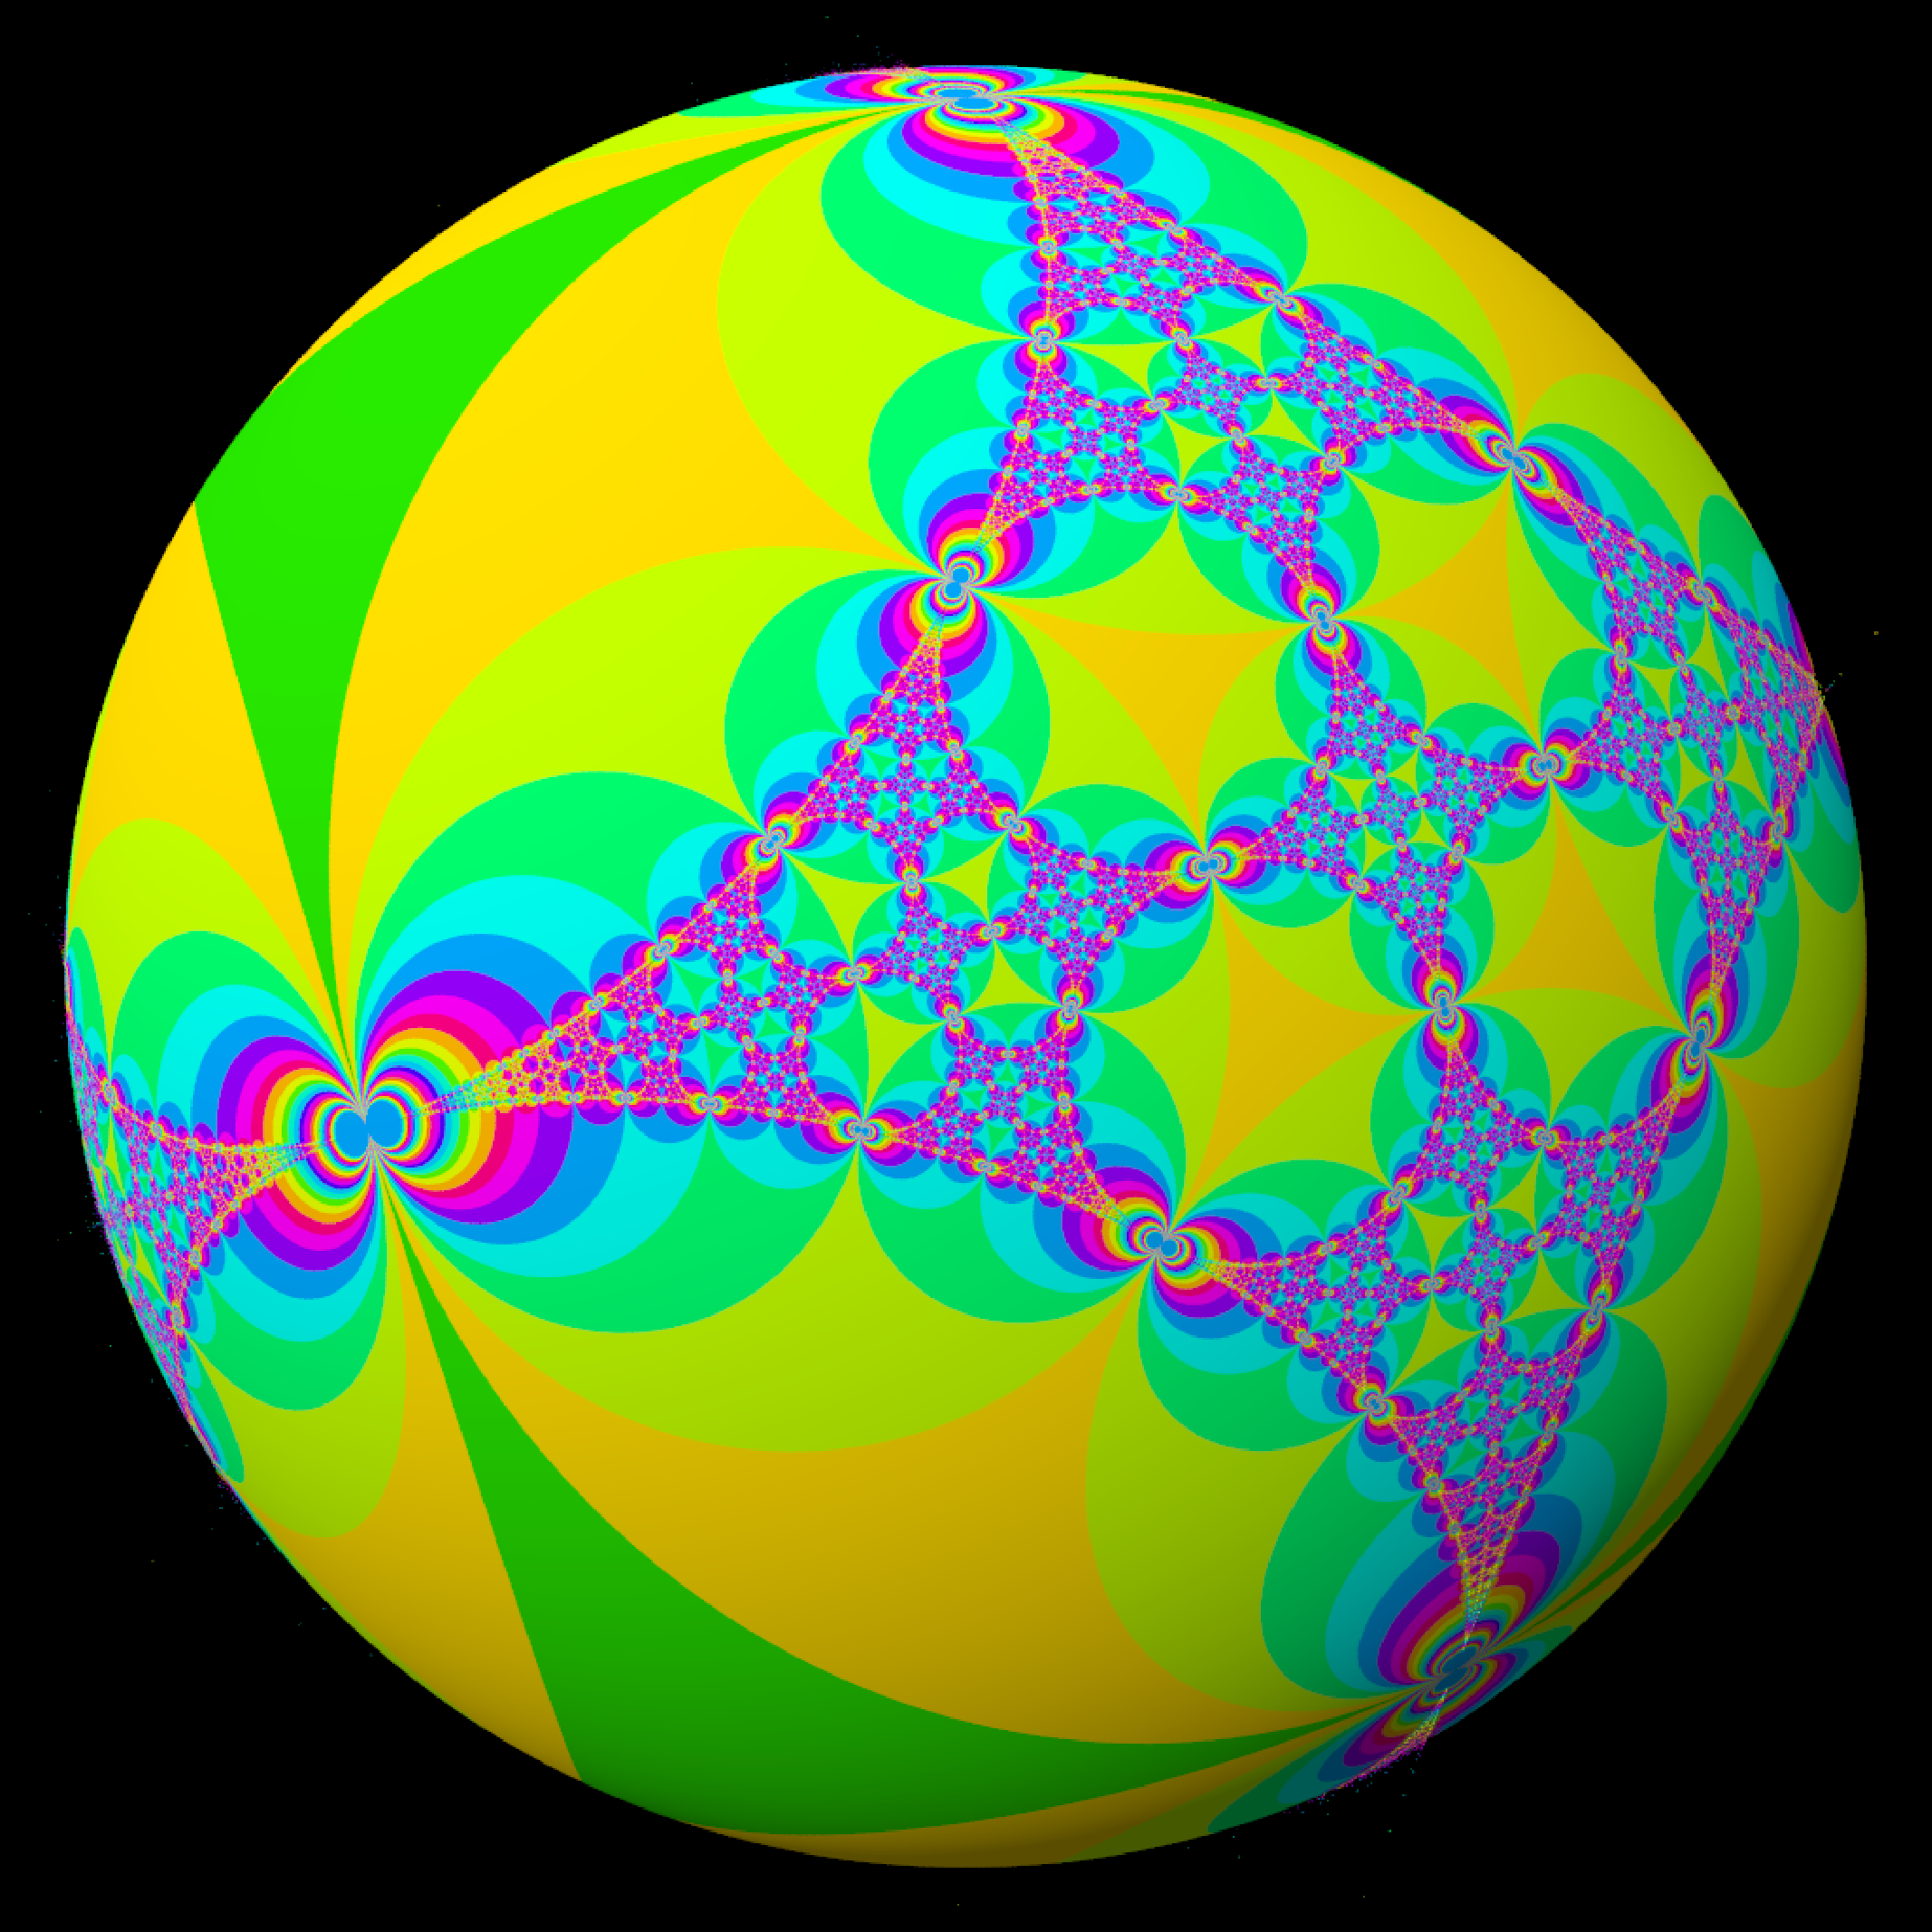
\includegraphics[ height=1.5in, keepaspectratio]{../img/klein/limitSetOnSphere.pdf}
   \subcaption{Orbit}
  \end{minipage}
  \hspace*{\fill}
  \caption{The limit set on the sphere}
  \label{fig:limitSetOnSphere}
 \end{minipage}
 \begin{minipage}{0.5\hsize}
  \begin{minipage}{0.24\hsize}
   \center
   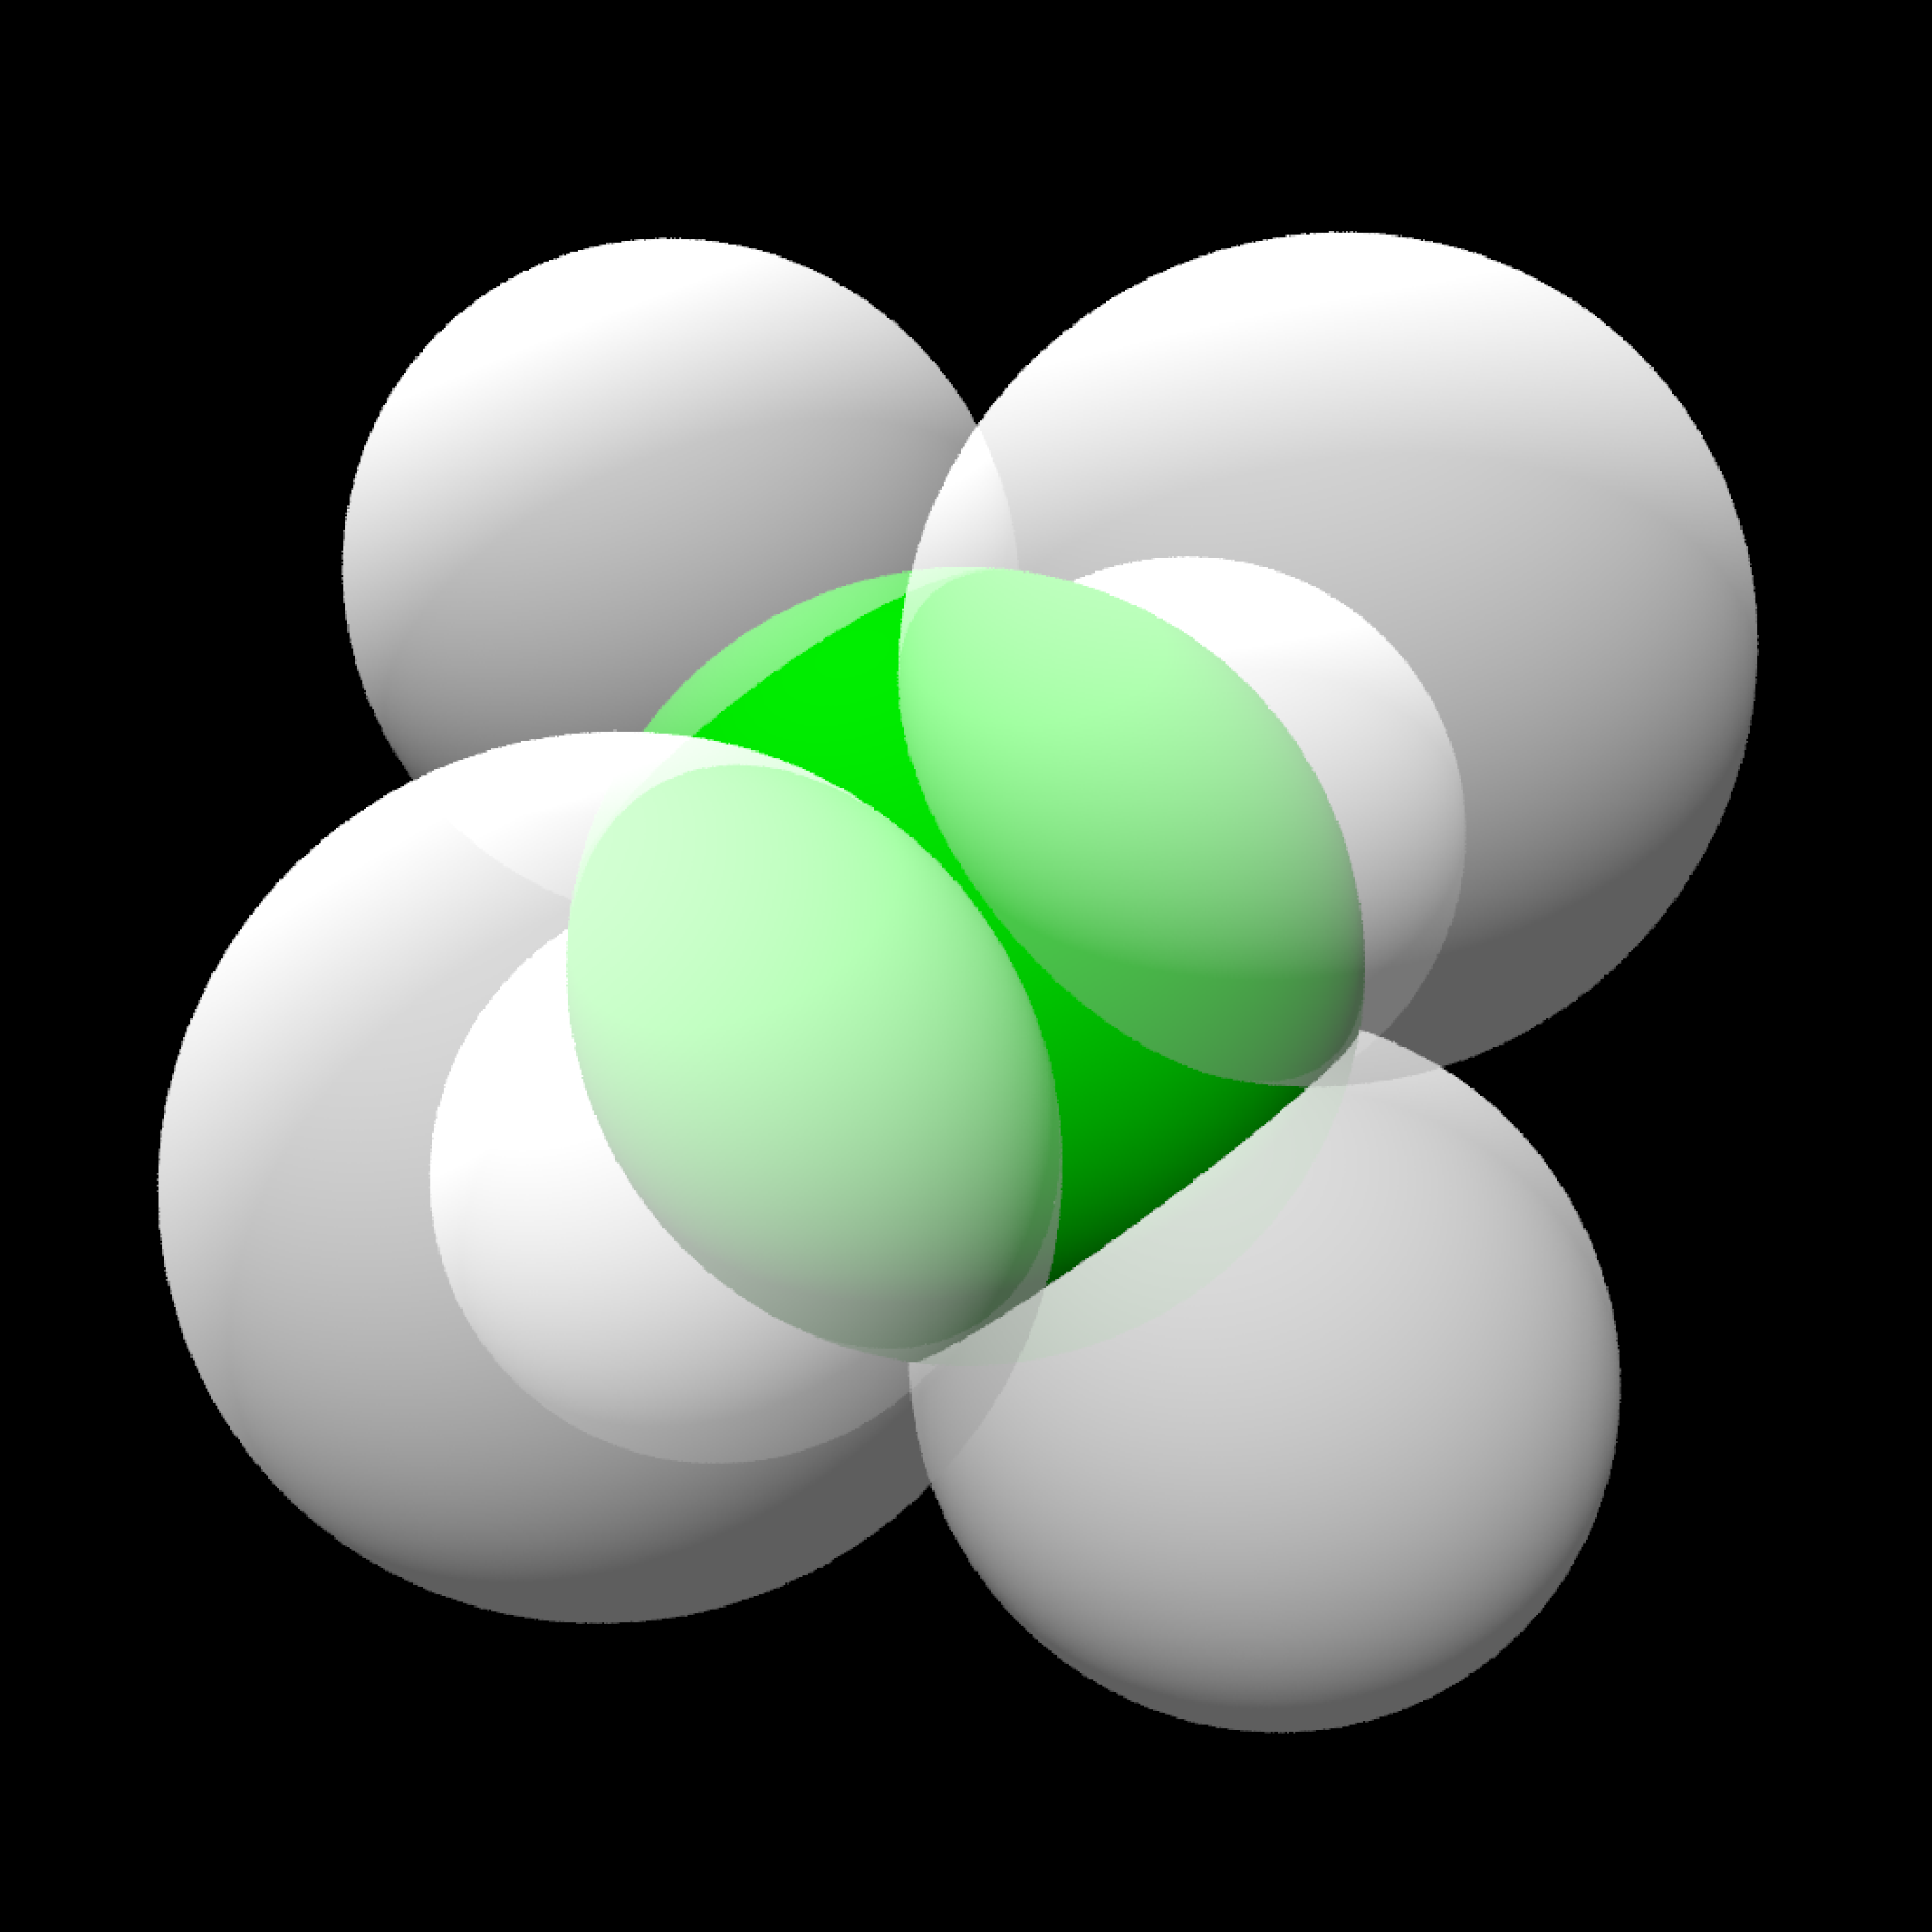
\includegraphics[ height=1.5in, keepaspectratio]{../img/klein/limitObjGen.pdf}
   \subcaption{Generator}
  \end{minipage}
 \hspace*{\fill}
  \begin{minipage}{0.24\hsize}
   \center
   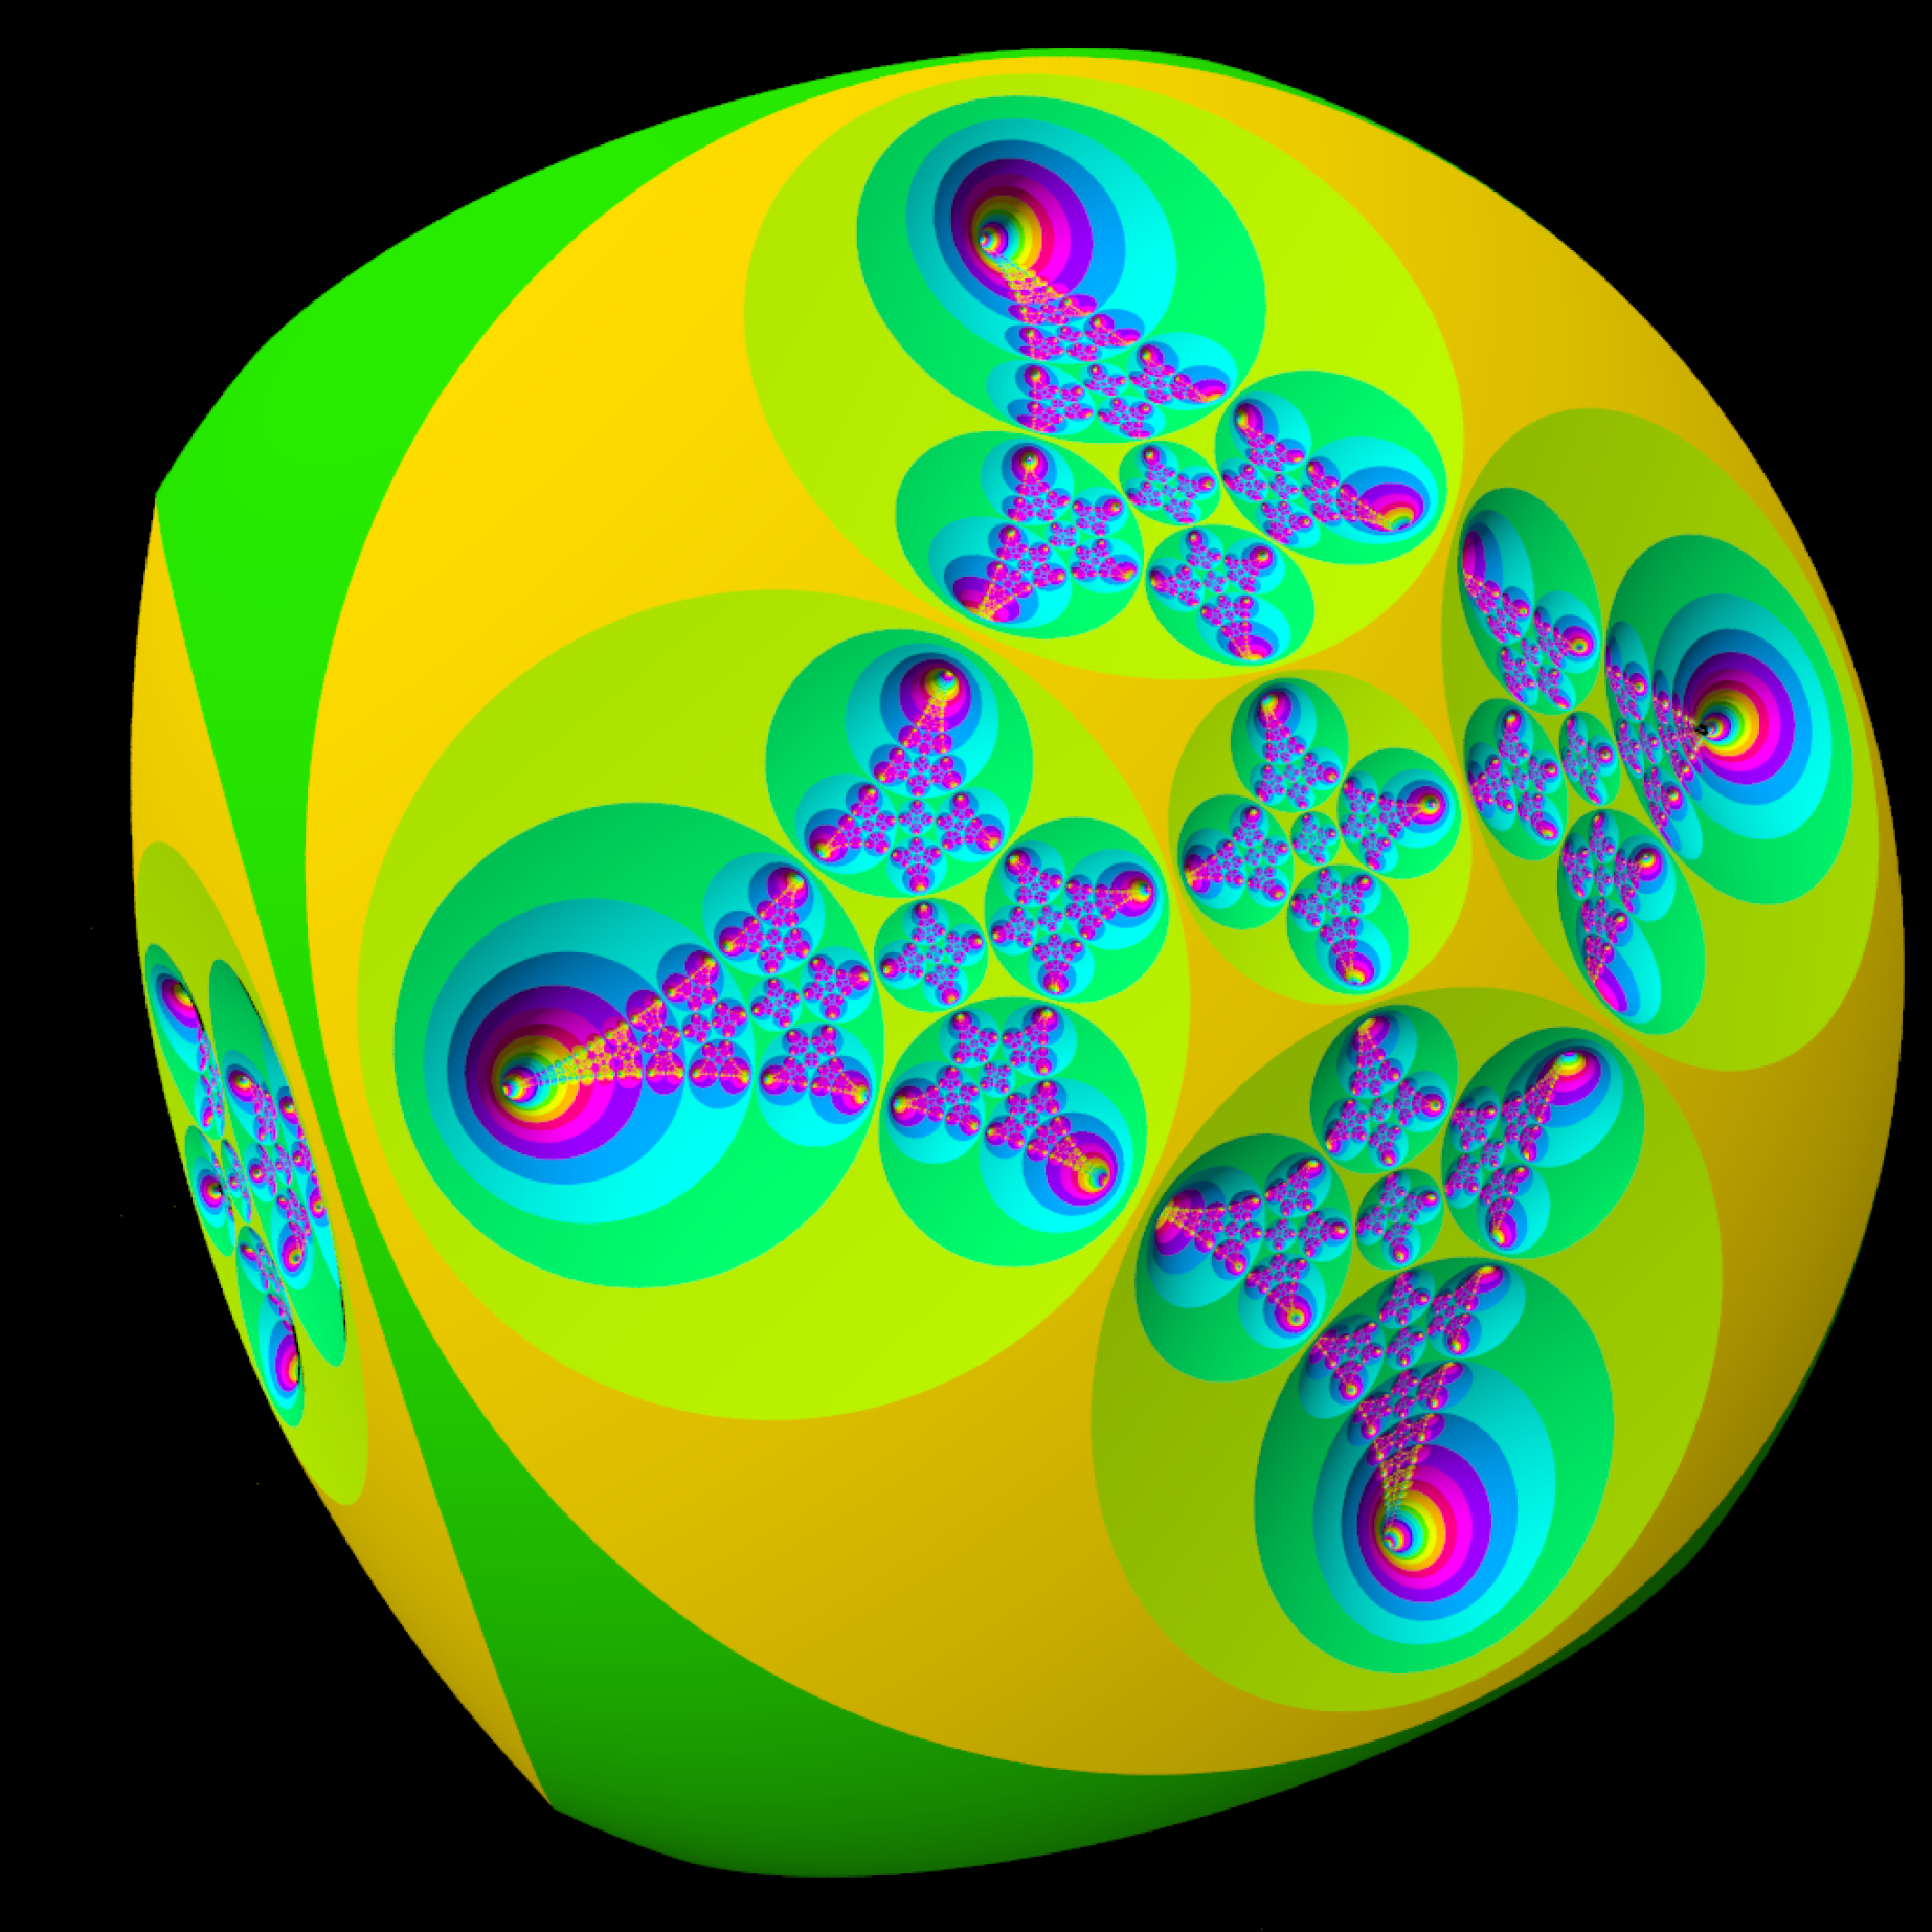
\includegraphics[ height=1.5in, keepaspectratio]{../img/klein/limitObj.pdf}
   \subcaption{Orbit}
  \end{minipage}
 \hspace*{\fill}
  \caption{More large radius}
  \label{fig:limitObj}
 \end{minipage}
\end{figure}

\begin{algorithm}
 \caption{Distance function}
 \label{alg:iis3d}
 \begin{algorithmic}
  \REQUIRE count $= 0,~d = $ \texttt{MAX\char`_DISTANCE} $,~dr = 1.0,~$and coordinates $=$ tipping
  point of the ray
  \FOR{$i=0$ to \texttt{MAX\char`_INVERSION}}
  \STATE inFundamentalDomain $\leftarrow$ \TRUE
  \FOR{ each Map $G$ in Maps}
  \IF{$G$ is available to coordinates}
  \STATE coordinates $\leftarrow$ $G(\text{coordinates})$
  \STATE $dr \leftarrow dr~*~$($Jacobian$ of $G(\text{coordinates})$)
  \STATE INCREMENT count
  \STATE inFundamentalDomain $\leftarrow$ \FALSE
  \ENDIF
  \ENDFOR
  \IF {isInFundamentalDomain}
  \STATE BREAK for
  \ENDIF
  \ENDFOR
  \FOR{ each BaseSphere $S$ in BaseSpheres}
  \STATE $d \leftarrow$ min($d,$~scalingFactor$~*~(distance$(coordinate$,~S.center$) $-$
  $S.radius$) $/$ (absolute value of $dr$))
  \ENDFOR
  \RETURN $d$
 \end{algorithmic}
\end{algorithm}

\subsection{Geometrical Representation of M\"obius Transformations}

多くの場合,メビウス変換は行列を用いて代数的に扱う.
しかし,行列表現でメビウス変換を操作することは直観が得にくい.
例えば,行列による変換の表現から変換の作用を推測することは非常に難しい.
このことは高次元のクライン群を扱う際に顕著となる.
三次元空間に作用するメビウス変換を考えることで,高次元のクライン群
を構成することができる.
このようなメビウス変換の軌道は,三次元空間での捻れを持ち,非常に興味深い
形状である.しかし,それらは四元数行列で表現されるため,さらに複雑な代数
計算が必要となる.

代数計算によって,クライン群の生成元のレシピを考案することは非常に難しい
研究テーマである.クライン群の極限集合の形状はアートとしてみても非常に魅
力的であるが,美しい極限集合を生成するオリジナルのレシピを作ることはアー
ティストにできることではない.

しかしながら,図\ref{fig:schottky}や図\ref{fig:simple3diis}に描かれるよ
うな,円や球の反転による軌道には,その形から幾何学的な直
観が働く.そのため,生成元と可視化される図形の間の関係を容易に理解するこ
とができる.そこで筆者はすべてのメビウス変換を円や球の反転で構成し,その
軌道を描くことを考えた.
群の軌道を描く処理は計算量が大きいものであったが,IISを用いることで複雑
な生成元をもつ群も高速に描くことができるようになった.
群の生成元を直観的に構成し,リアルタイムに可視化することは研究者だけでな
く,フラクタルアーティストにも有益なことである.

この節では,二次元と三次元のメビウス変換を円と球の反転の合成で構成し,そ
の軌道をIISで描画するための手法をまとめる.この内容は\textit{Bridges
2017}に投稿中である.
また,筆者は円や球の反転で構成される群をインタラクティブに構成するウェブアプリ
ケーション,{\it Schottky Link} \footnote{Schottky Link:
\url{https://schottky.jp}}を開発している.

\subsubsection{2D Generators}

まずは二次元の生成元からみていく.
複素平面に作用するメビウス変換は円の反転を合成することで構成することがで
きる.二次元の群は反転円自身の軌道を描画することで可視化する.

\noindent\textbf{Simple Inversion.}

先に述べたように,円に関する反転は複素平面の向きを変えるので,メビウス変
換ではない.
二つの反転円がペアとなってはじめてメビウス変換となるため,偶数個の円が必
要である.
しかし,アルゴリズム上は奇数個の円の反転による群も可視化することができる
ので,一つの円の反転もメビウス変換として扱うことにする.

二つの円をペアにする変換は特に\emph{ショットキー変換}(\textit{Schottky
transformation})とよばれる.
ショットキー変換は片方の円の外側をもう片方の円の内側へと移す変換であり,
これは円の反転と同一視することができる.
また,円のペアによるショットキー変換で構成された群を\emph{古典的ショット
キー群}(\textit{classical Schottky groups})とよぶ.

\noindent\textbf{Inversion of a Circle with Infinite Radius.}

無限の半径をもつ円はその円弧を直線として表すことができるので,その反転は
直線に関する反転として扱うことができる.
図\ref{fig:infCircle}では中央の直線による反転で,左右対称の軌道をみること
ができる.

\noindent\textbf{Rotation.}

二つの交差する直線の反転の組み合わせは回転を表わす.回転角は二直線のなす
角の二倍である.図\ref{fig:rotation}において,二直線は45度で交わっている
ので90度回転を表している. また,軌道の円同士がお互いに
重なりあわないようにするためには,回転角は有理角である必要がある.

\noindent\textbf{Parallel Translation.}

平行な二直線による反転の組は直線の垂直方向への平行移動を表す.
図\ref{fig:translation2d}では二つの無限の半径をもつ円が向かい合っている.
これらの円の反転が繰り返されることにより,中央の4つの反転円はX軸方向に
平行移動される.
平行移動の固定点は無限遠点であり,これは放物型変換となる.

\begin{figure}[h!tbp]
 \begin{minipage}[t]{0.3\hsize}
  \center
   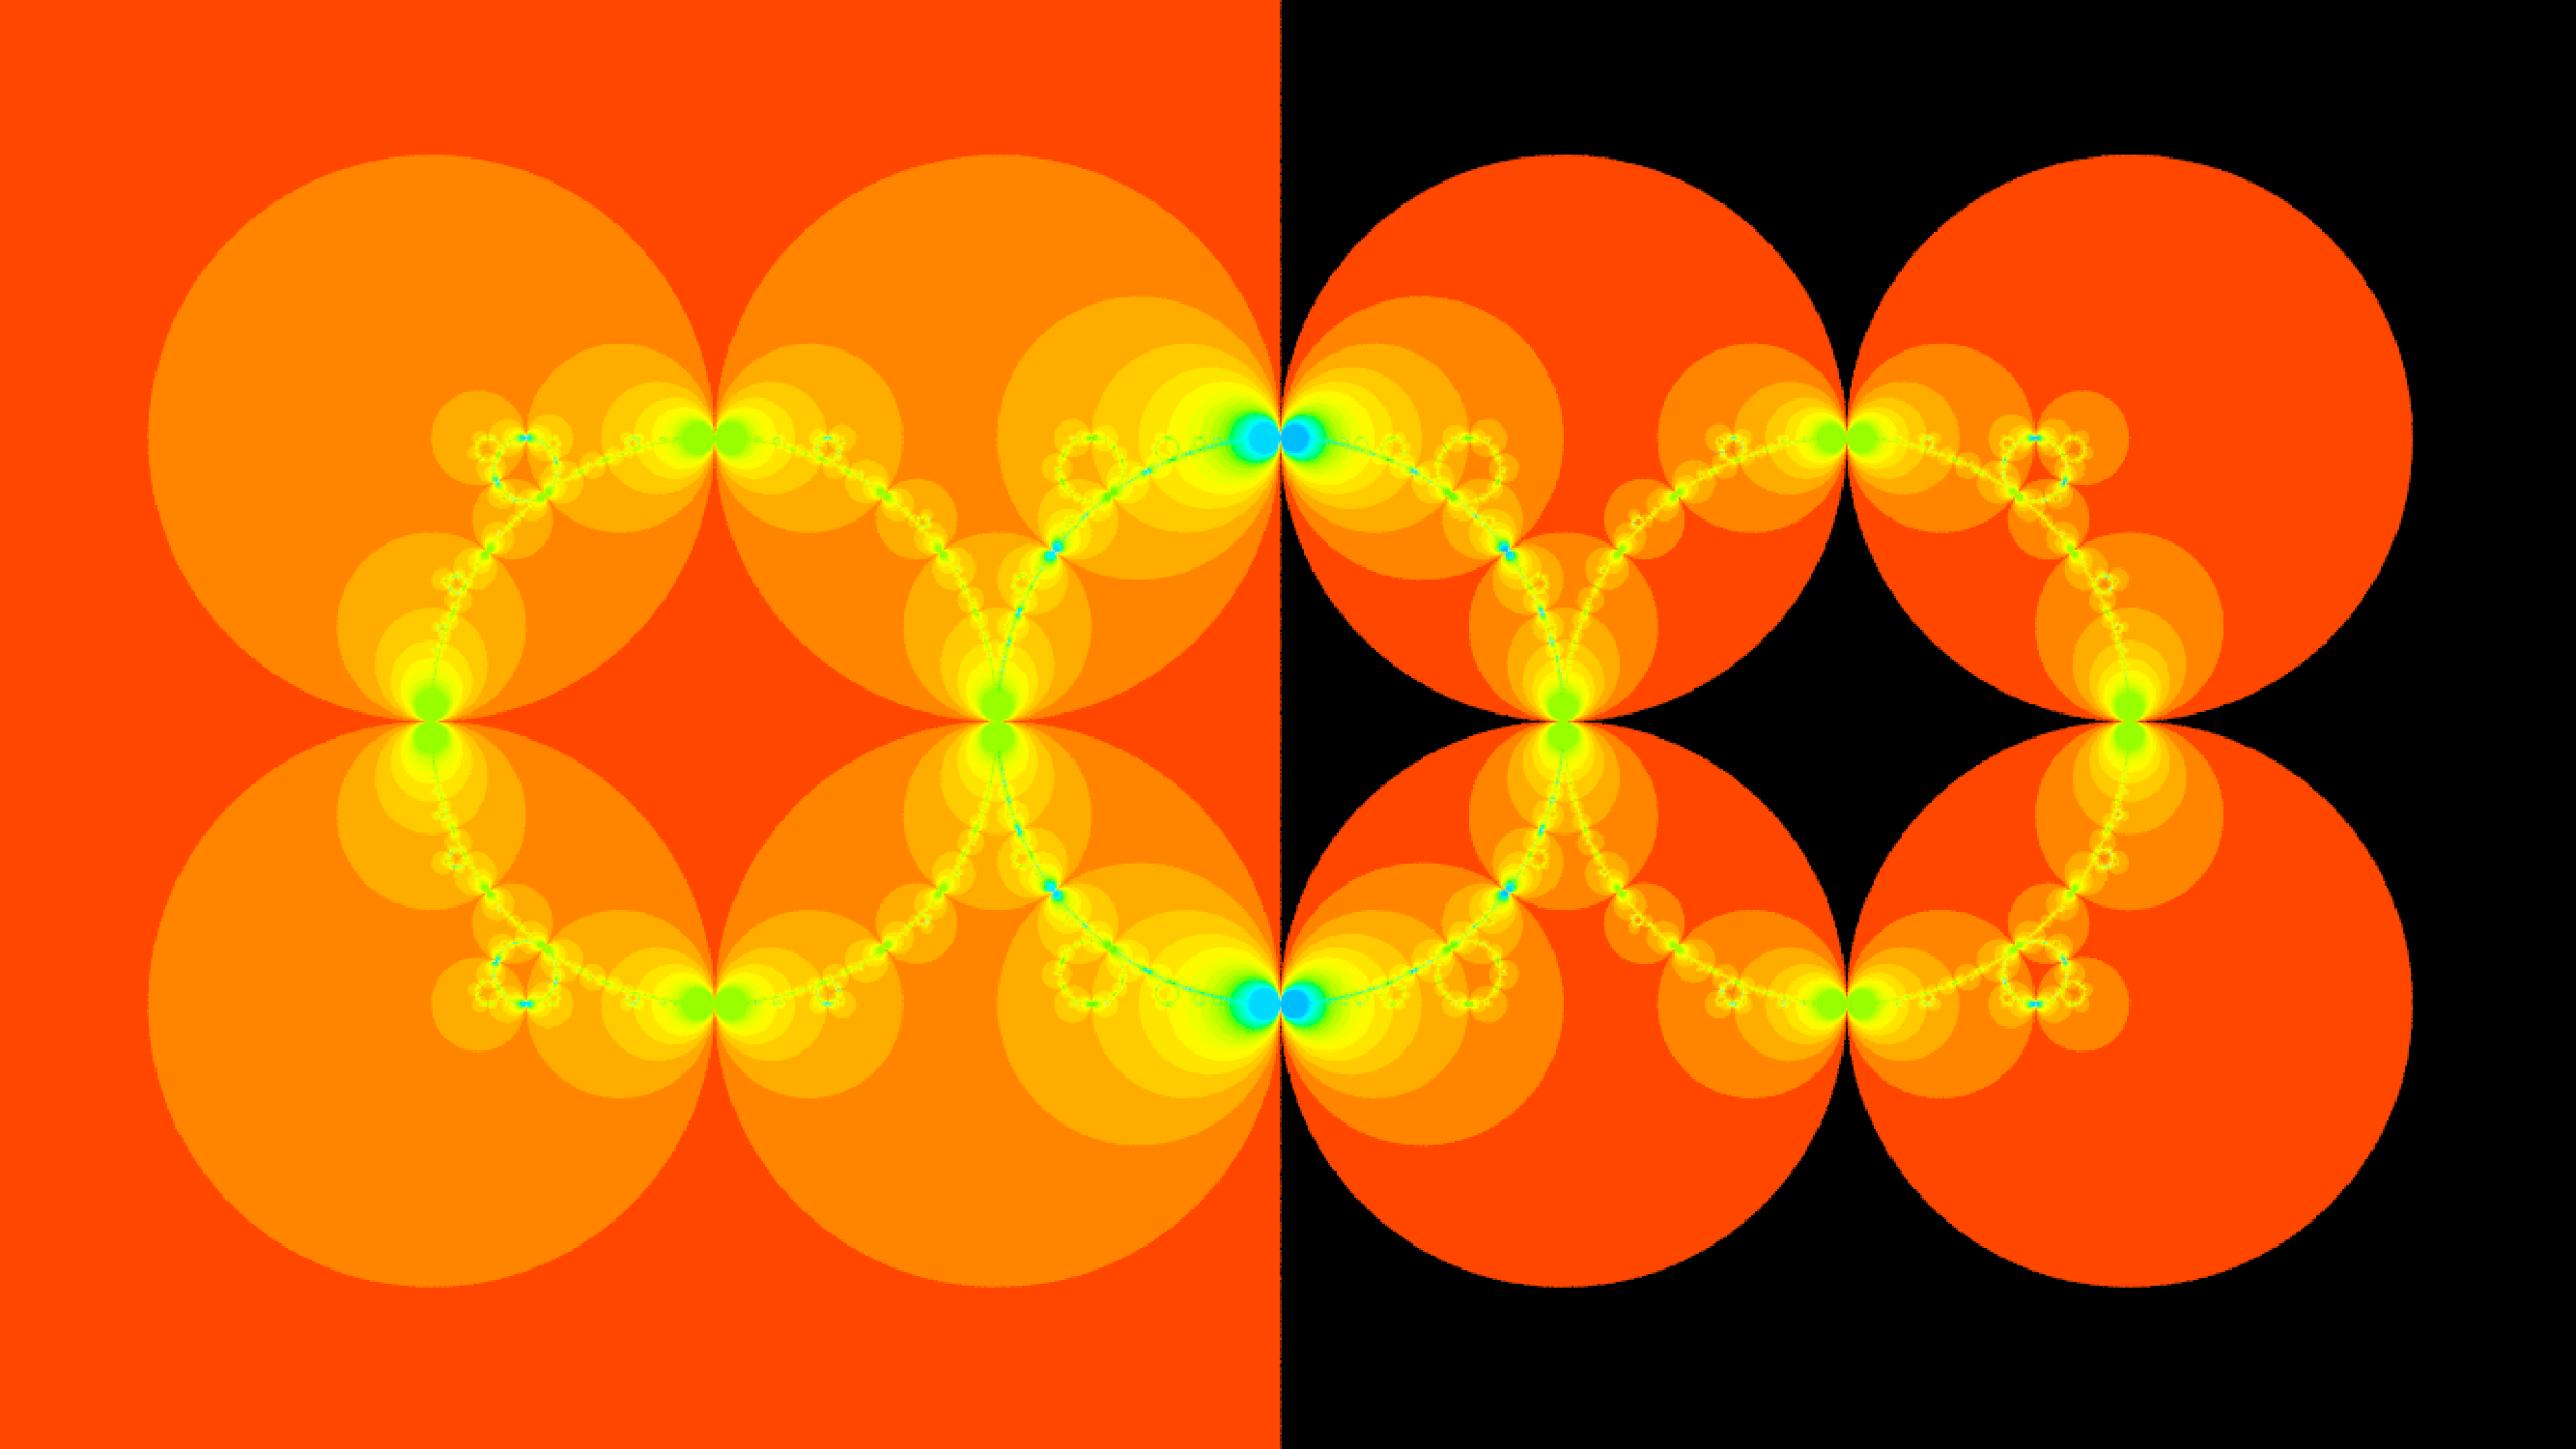
\includegraphics[width=2in, height=2in, keepaspectratio]{../img/klein/2diis/infCircle.pdf}
  \caption{Inversion of the circle with infinite radius}
  \label{fig:infCircle}
 \end{minipage}
 \hspace*{\fill}
 \begin{minipage}[t]{0.3\hsize}
  \center
  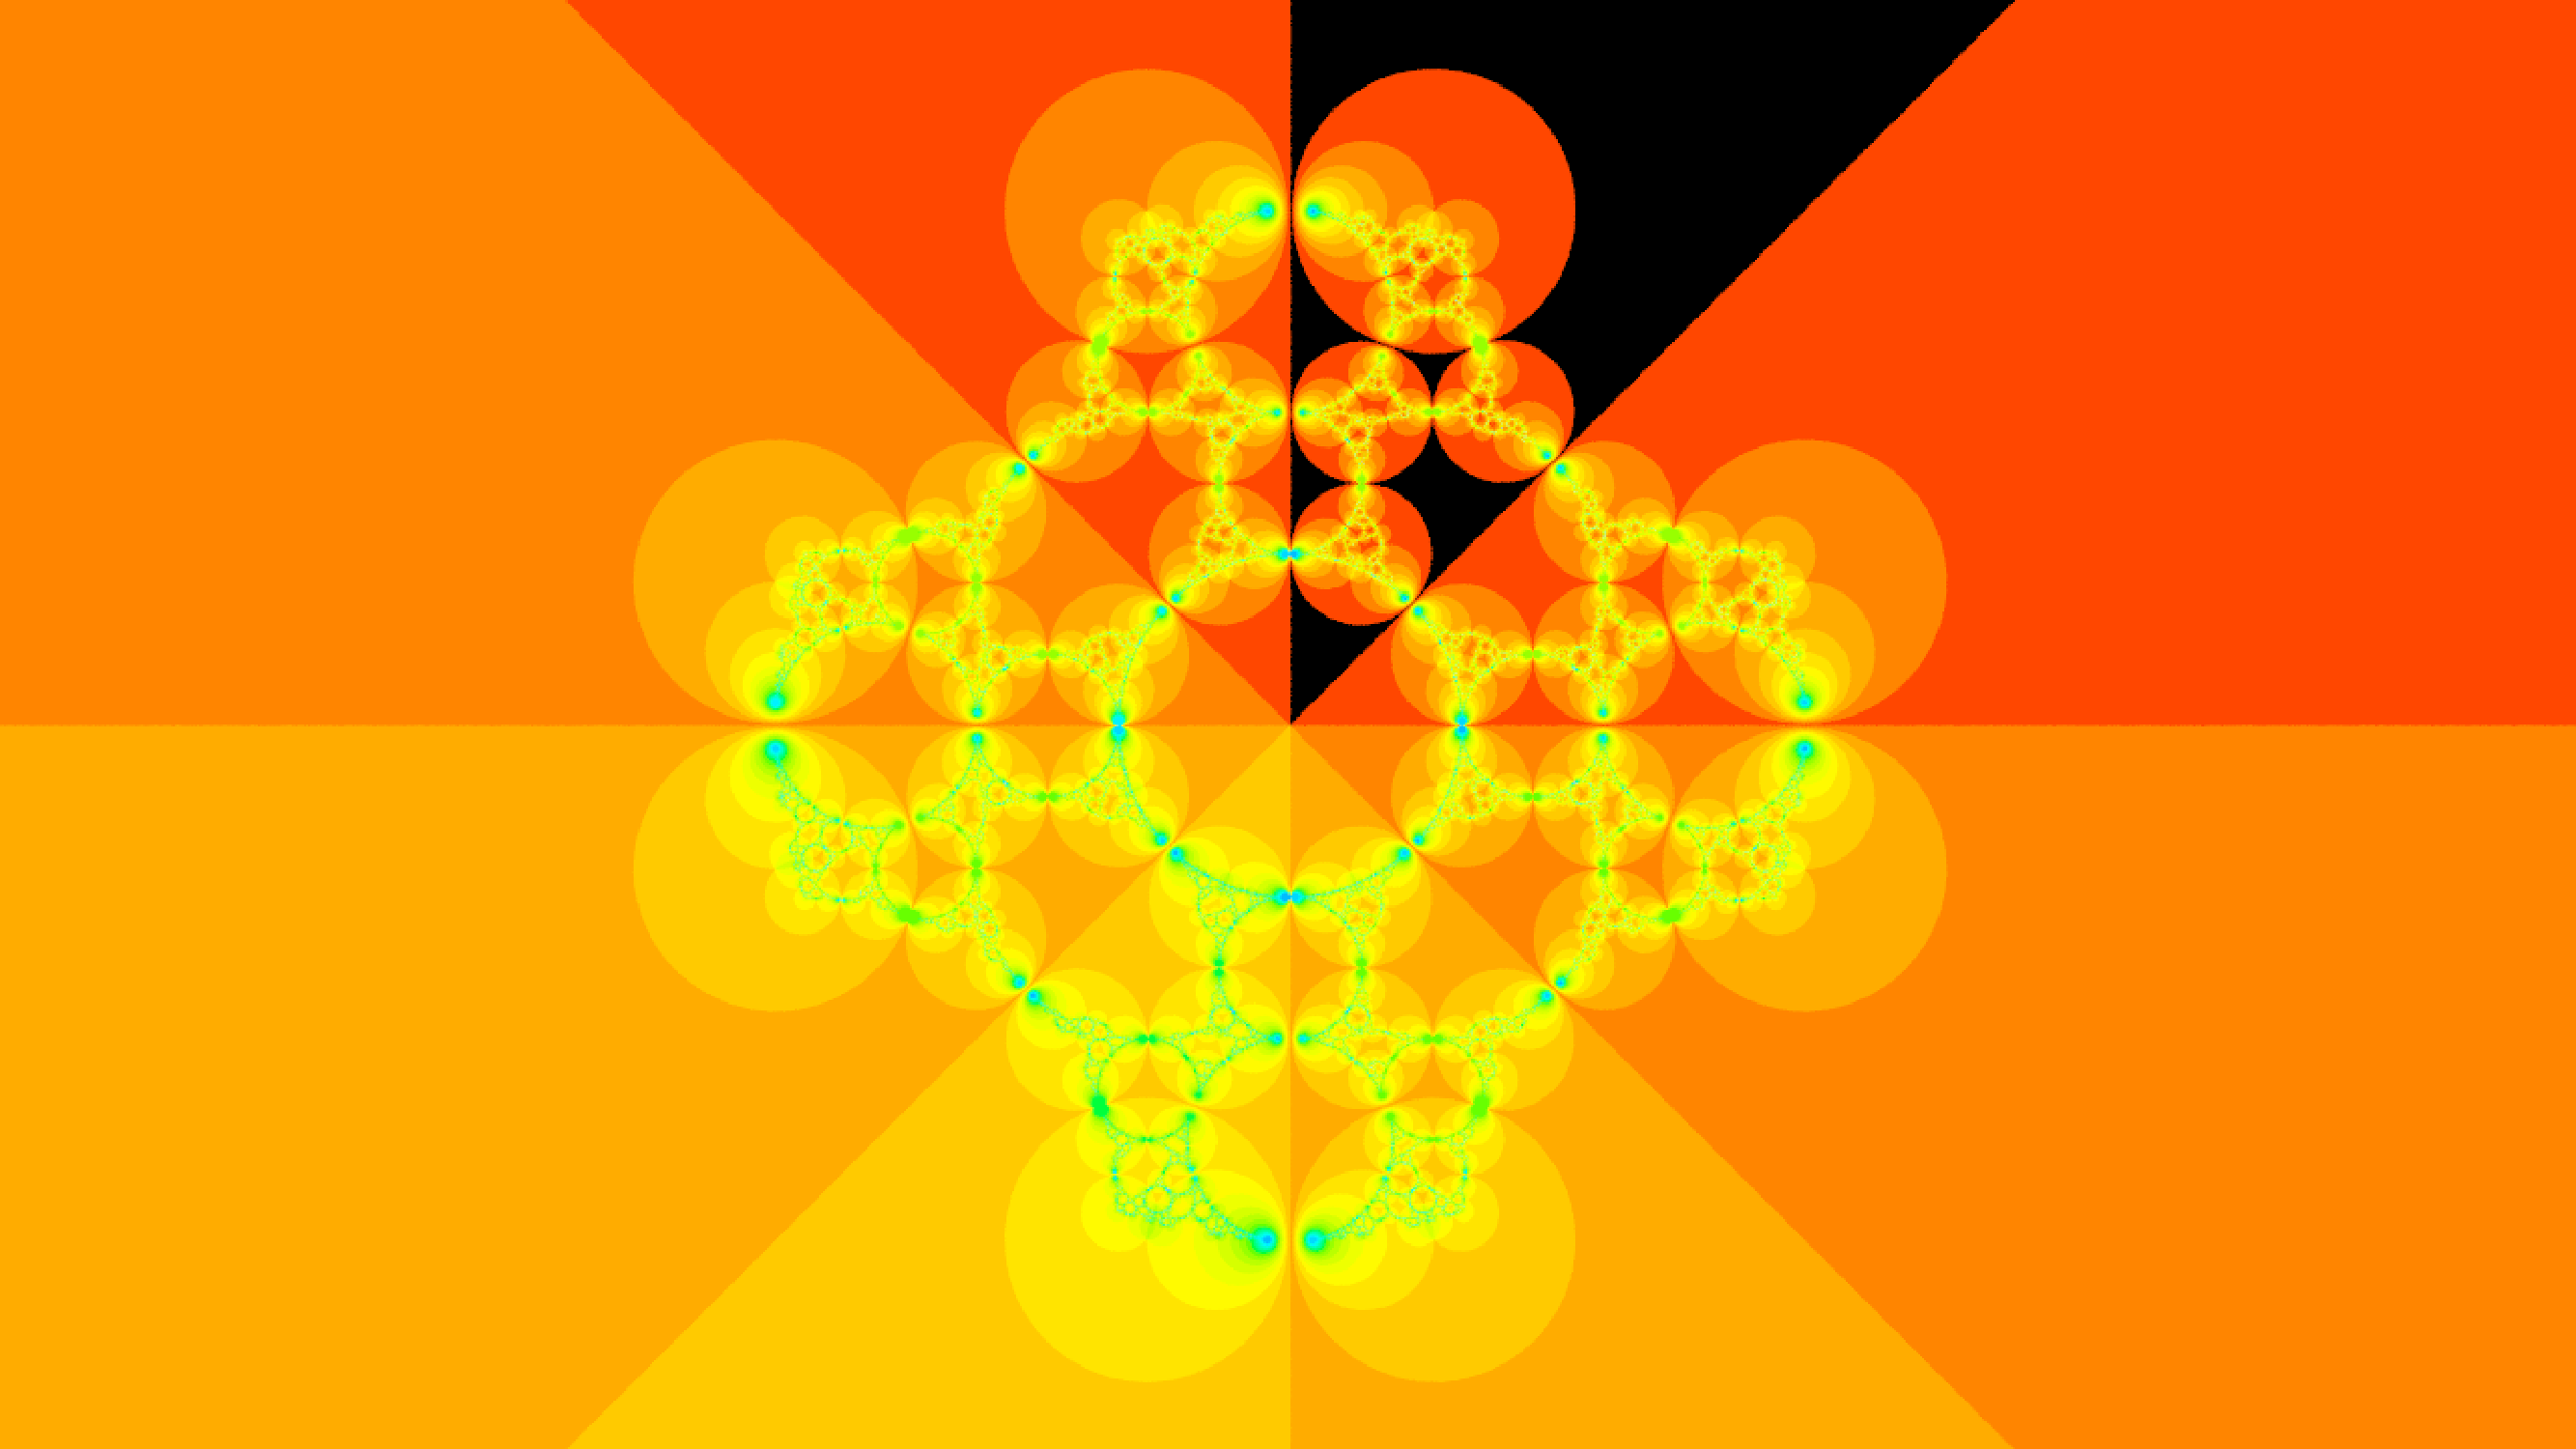
\includegraphics[width=2in, height=2in, keepaspectratio]{../img/klein/2diis/rotation.pdf}
  \caption{Rotation}
  \label{fig:rotation}
 \end{minipage}
 \hspace*{\fill}
 \begin{minipage}[t]{0.3\hsize}
  \center
  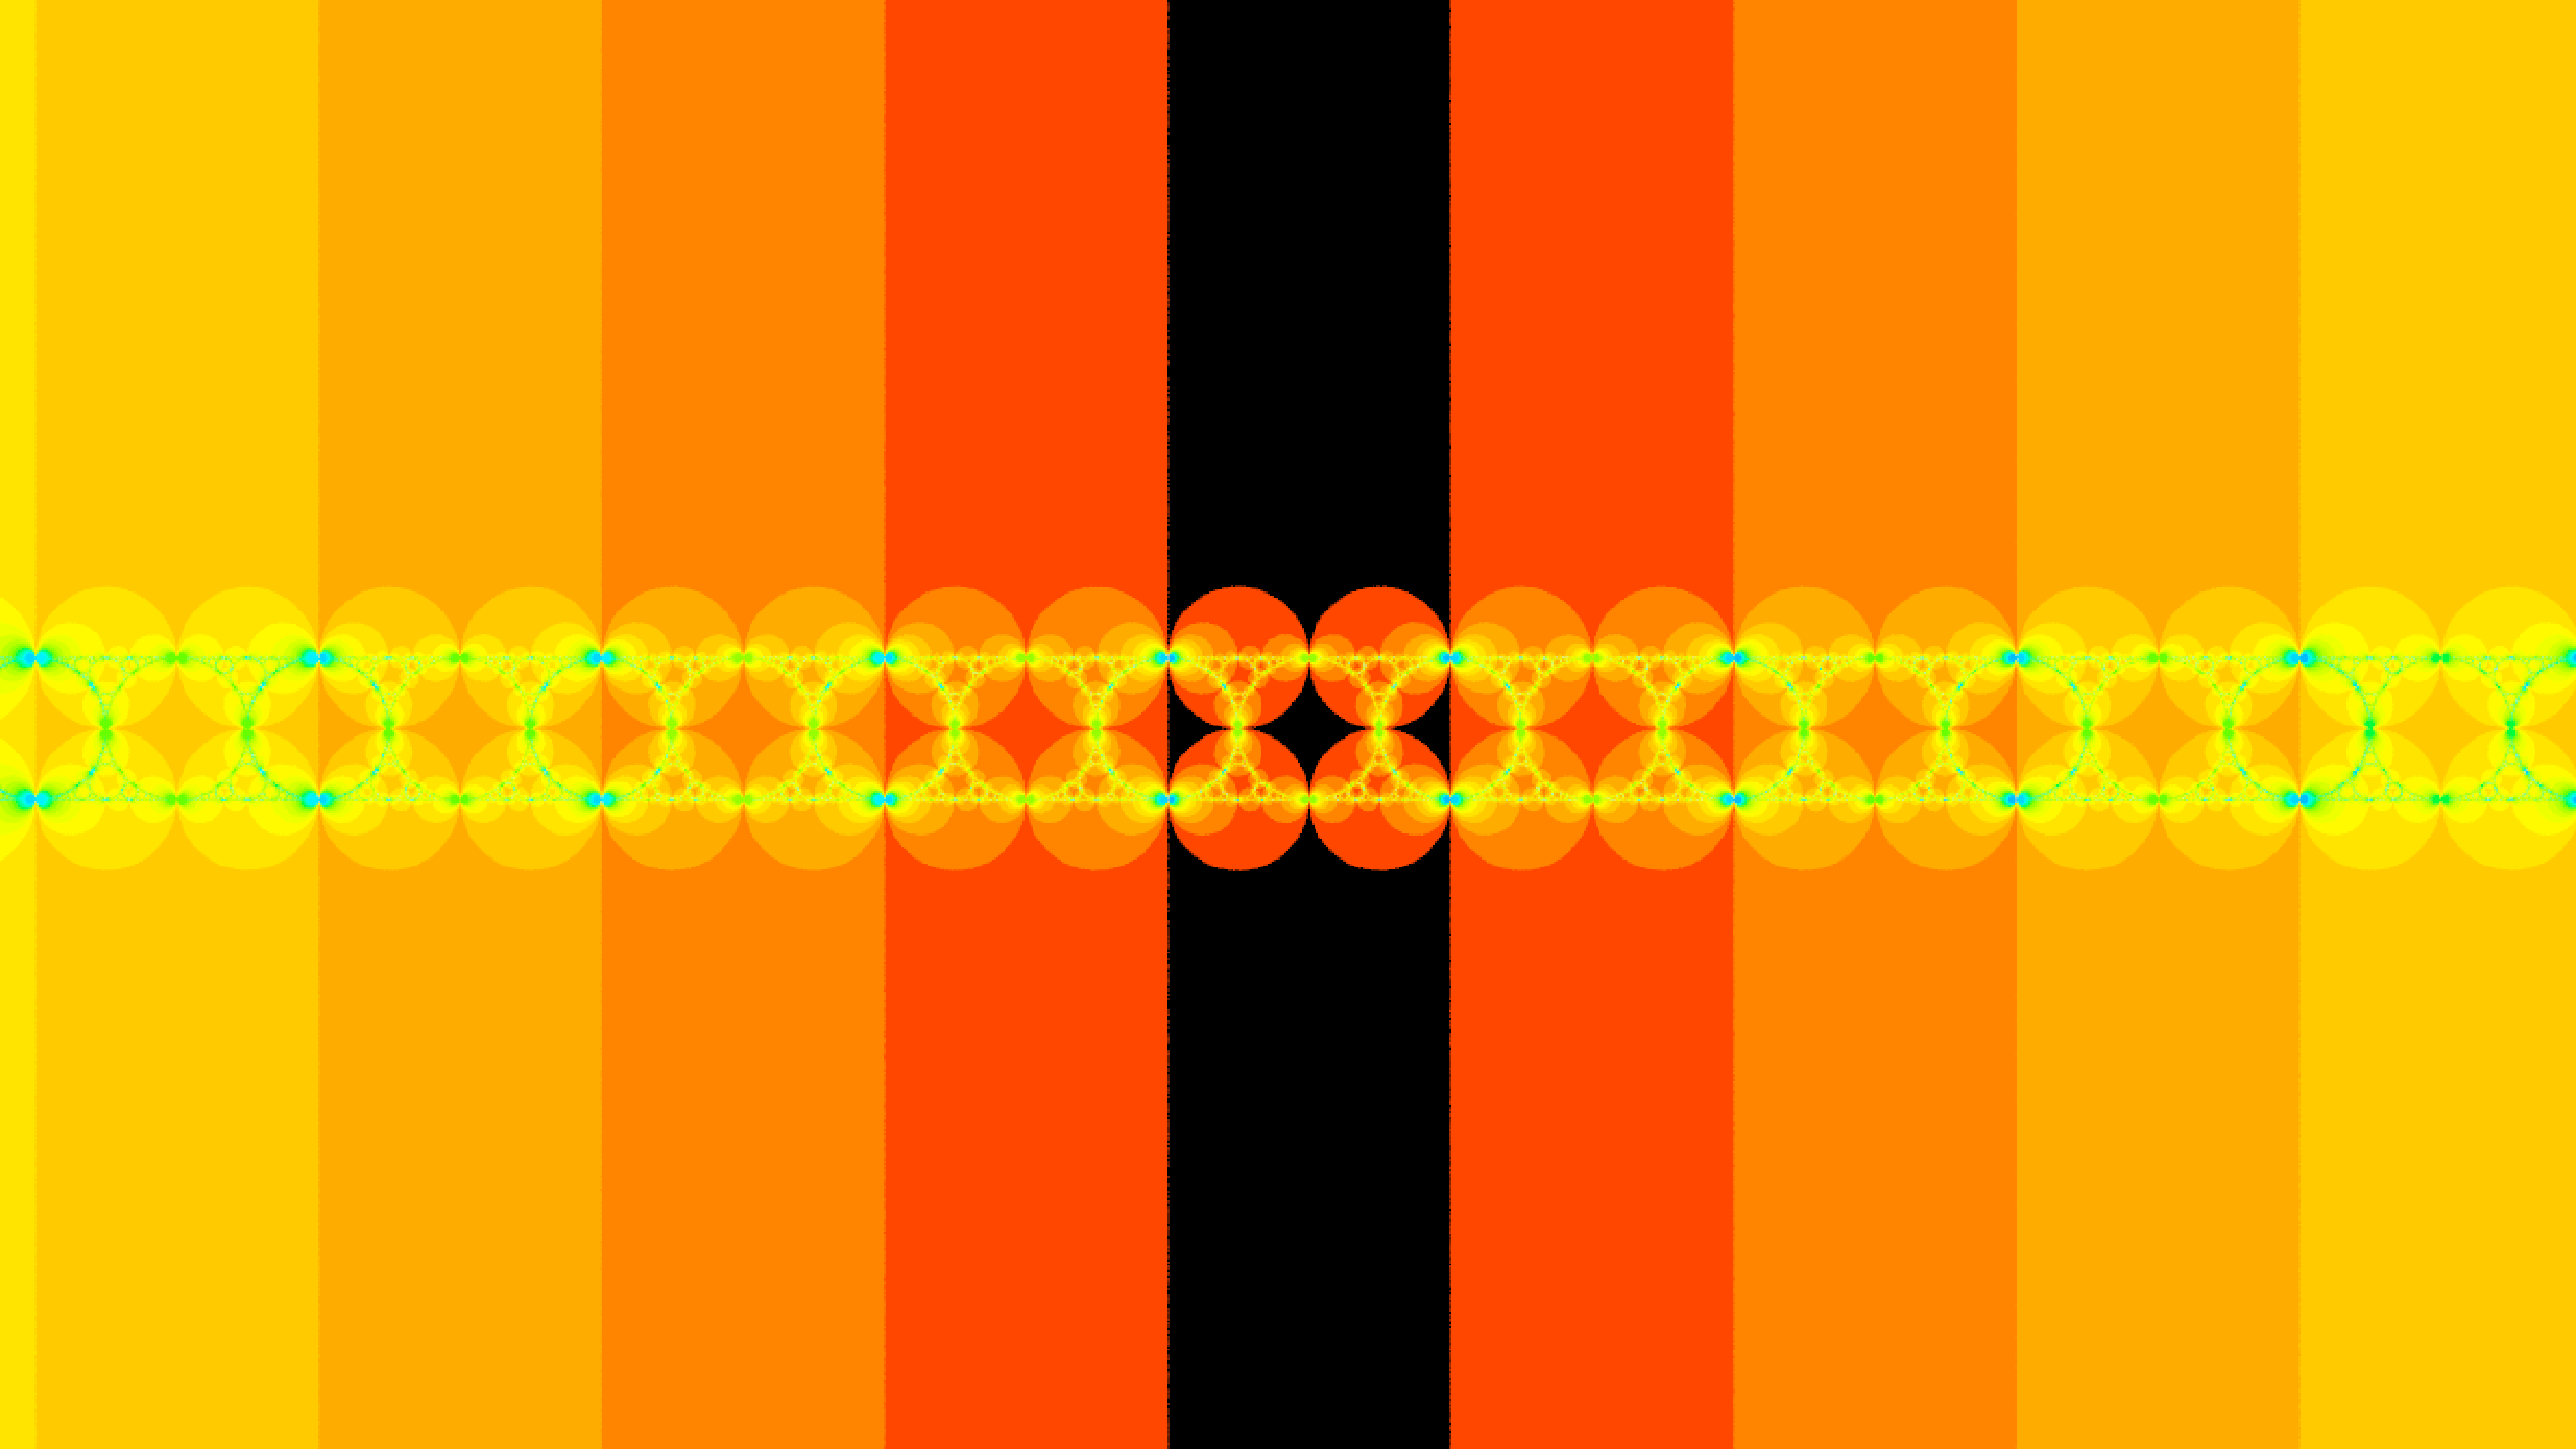
\includegraphics[width=2in, height=2in, keepaspectratio]{../img/klein/2diis/translation.pdf}
  \caption{Parallel translation}
  \label{fig:translation2d}
 \end{minipage}
\end{figure}

\noindent\textbf{Composition of Two Circles.}

二つの同心円による反転を合成することで,実数倍による拡縮
を表すことができる.これは双曲型変換となる.
図\ref{fig:scaling2d}における赤の円を$C1$,緑の円を$C2$,そして青の円を
$C1'$とよぶ.ここで$C1'$は$C1$を$C2$による反転で移した像である.
図\ref{fig:scaling2d}では,白い縁をもつ二つの円の軌道を描いている.
固定点は円の中心と無限遠点である.

IISに用いる写像$G$は以下のように定義される.
また,接頭辞$I$は反転を表わす.
例えば,$I_{C1}$は$C1$による反転を表わす.
\begin{align*}
 G =
  \begin{cases}
   I_{C2} \circ I_{C1} & (\text{The point is inside of } C1) \\
   I_{C1} \circ I_{C2} & (\text{The point is outside of } C1')
  \end{cases}
\end{align*}
$G$を点に繰り返し作用させることで,その点を基本領域へと移動させることができる.
この種類の生成元の基本領域は図\ref{fig:scaling2d}における青と緑の領域で
ある.つまり$C1'$の内側かつ$C1$の外側の領域である.
完全な円の軌道をIISを用いて描くには,反転円をこの領域内に配置す
る必要がある.

次に,$C1$を少し動かすと,図\ref{fig:hyperbolic2d}のような軌道が得られる.
無限遠点の固定点は有限の点に移り,有限の固定点は,$C1$の内部で移動する.
二つの円が交差しない限り,これも双曲型変換である.

$C1$と$C2$が接触する時,図\ref{fig:parabolic2d}のように固定点はその交点で重なりあい,放物型変換となる.

\begin{figure}[htbp]
  \begin{minipage}[]{0.3\hsize}
   \center
   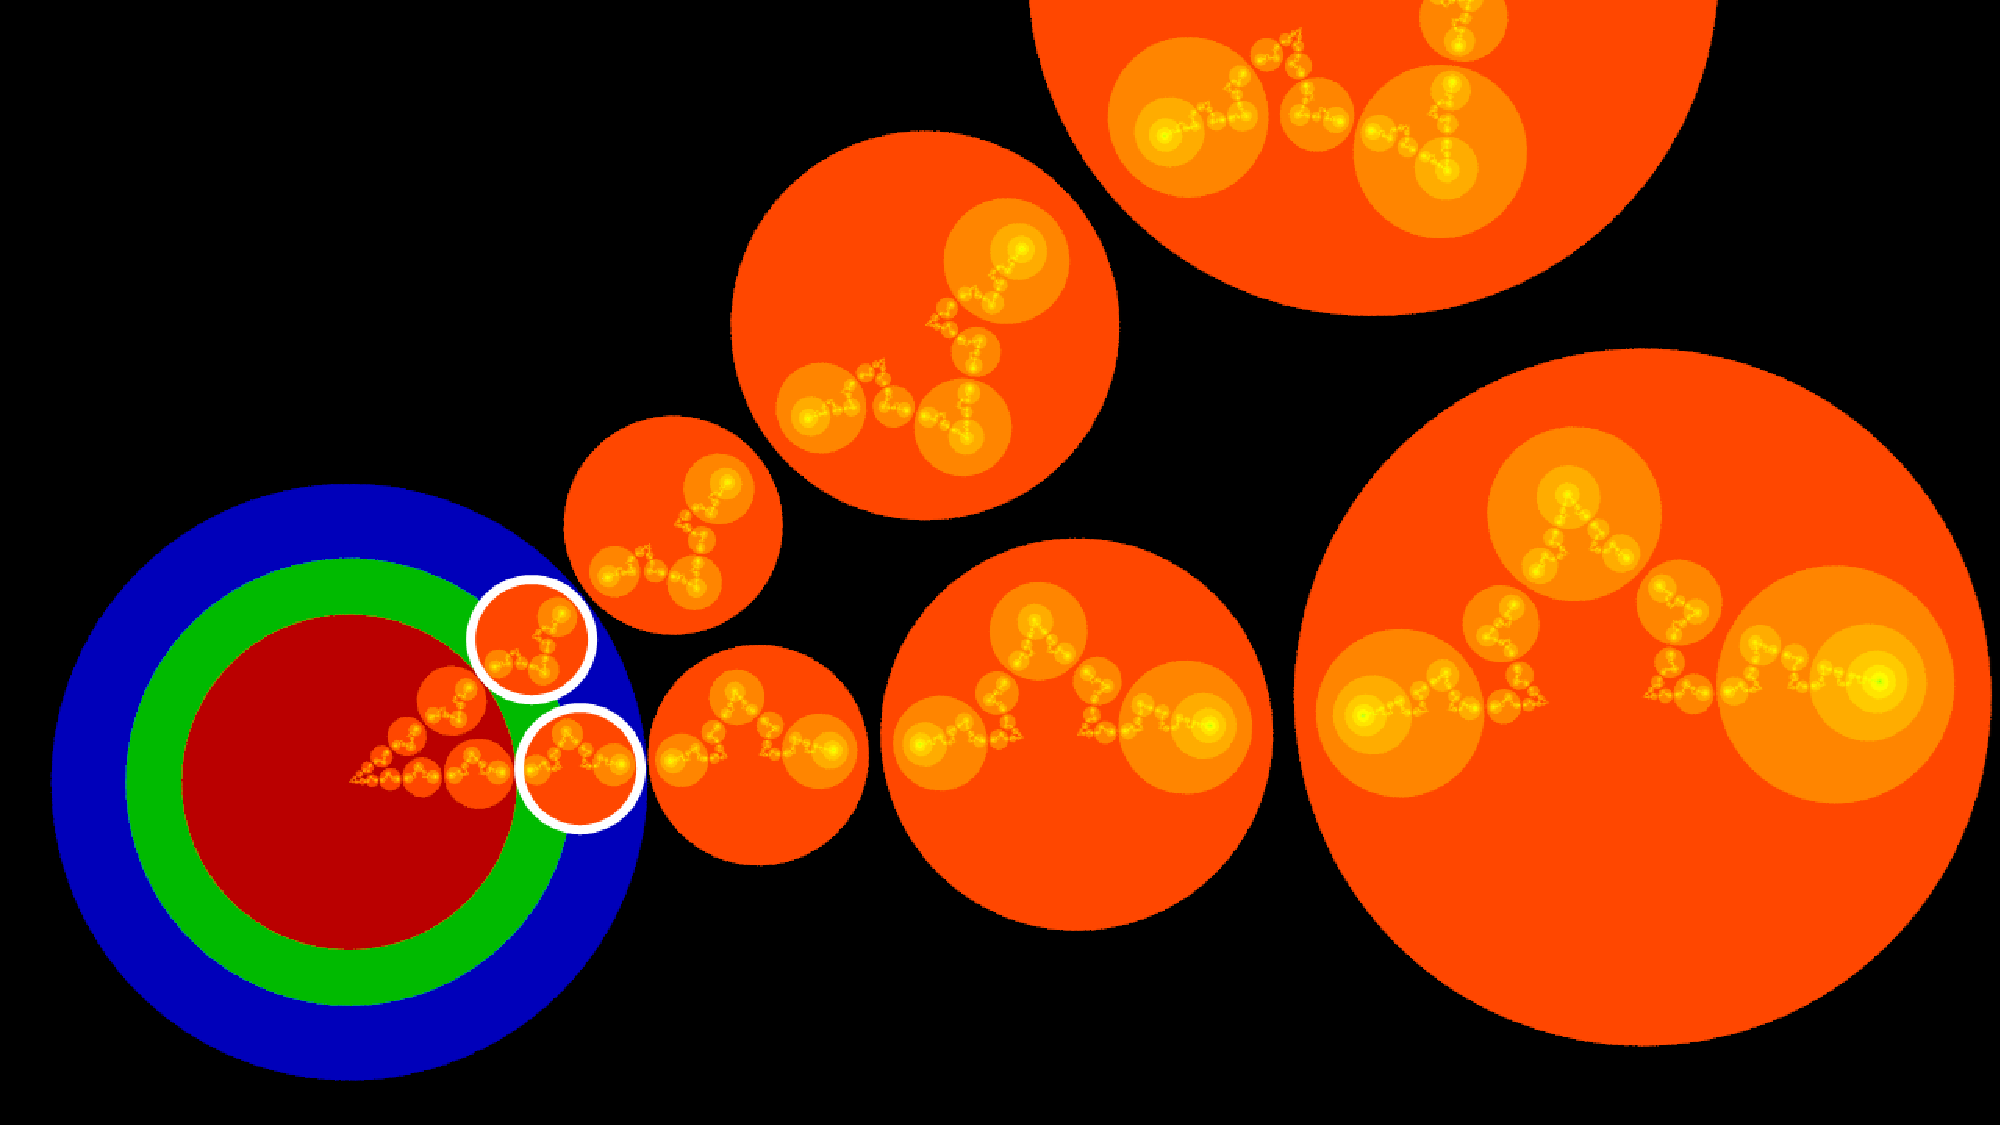
\includegraphics[width=2in, height=2in, keepaspectratio]{../img/klein/2diis/scaling.pdf}
   \subcaption{Scaling}
   \label{fig:scaling2d}
  \end{minipage}
 \hspace*{\fill}
  \begin{minipage}[]{0.3\hsize}
   \center
   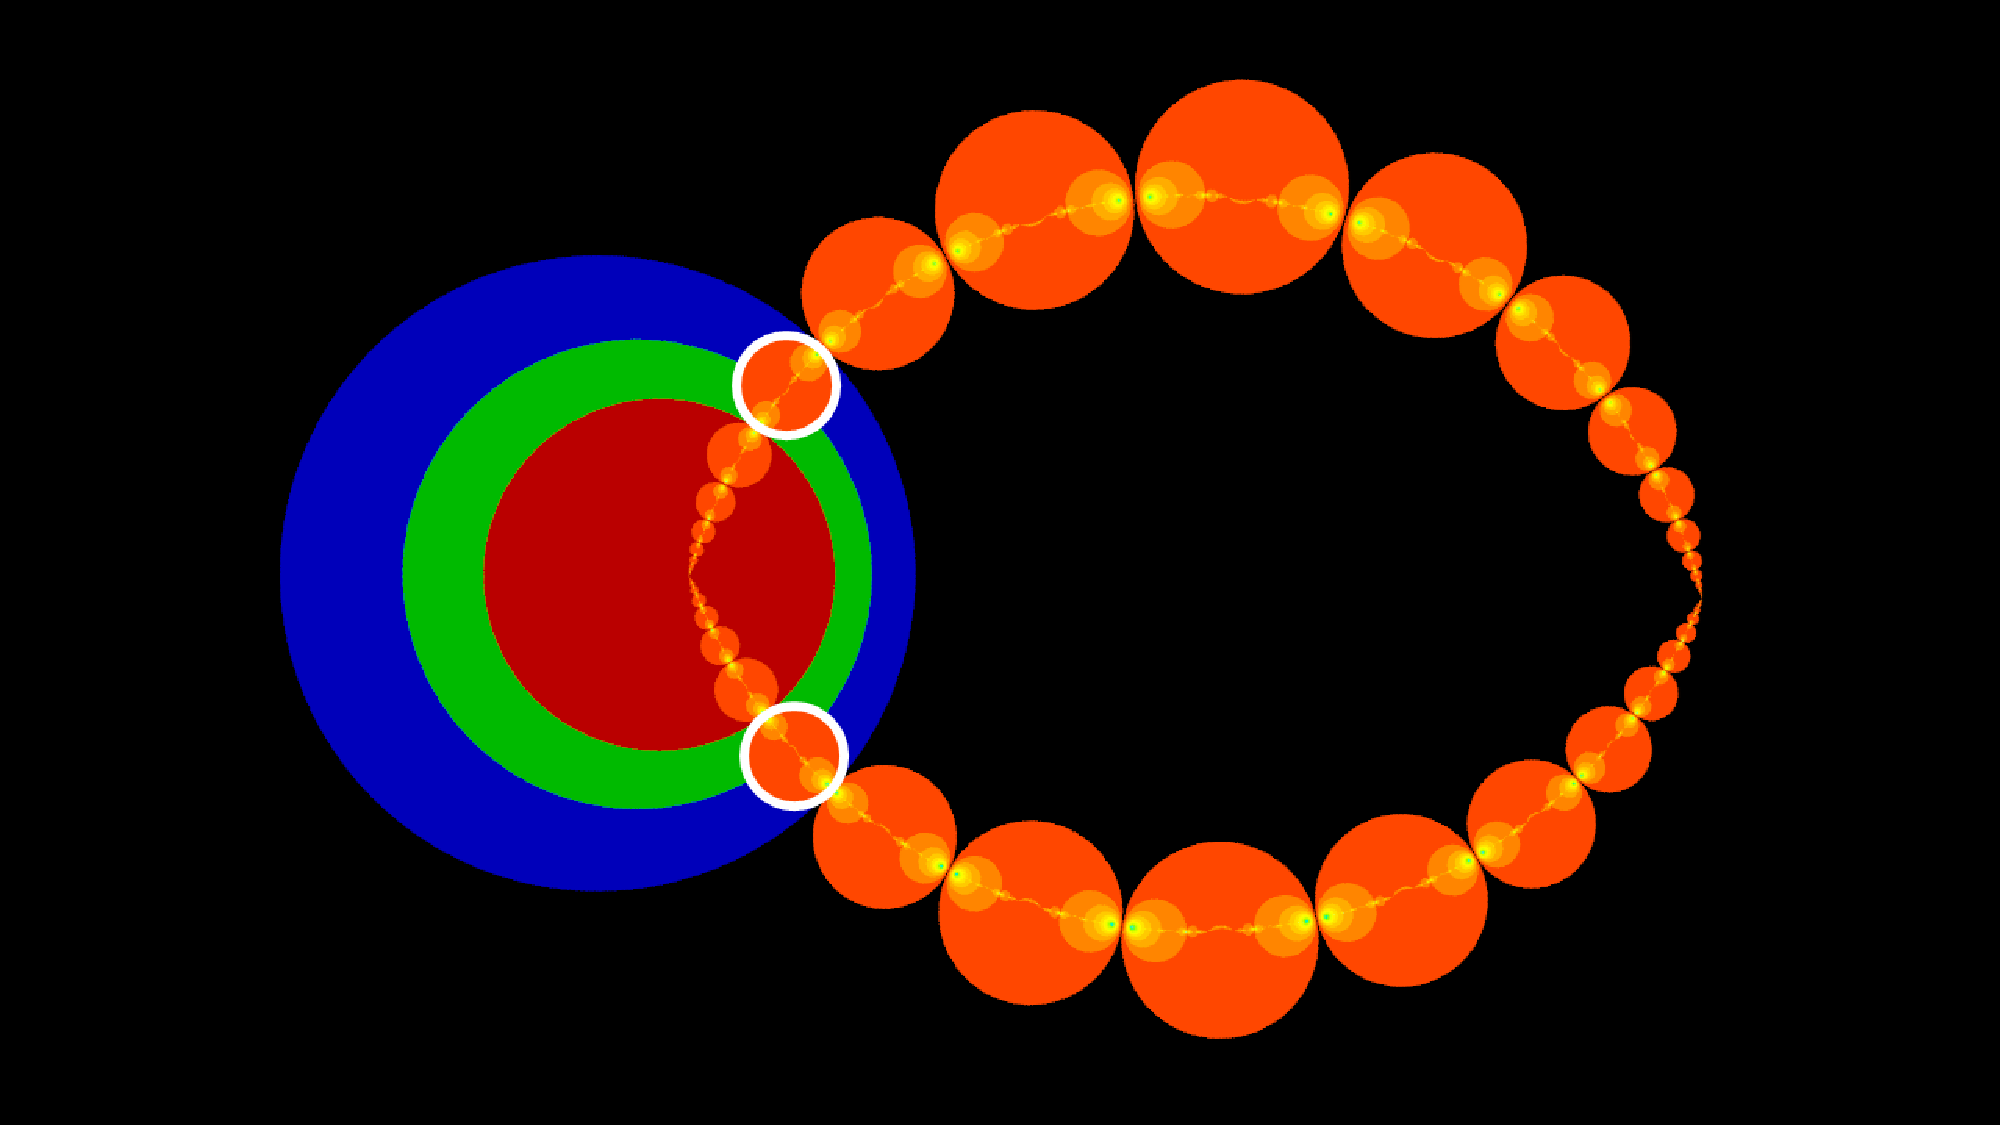
\includegraphics[width=2in, height=2in, keepaspectratio]{../img/klein/2diis/hyperbolic.pdf}
   \subcaption{Hyperbolic}
   \label{fig:hyperbolic2d}
  \end{minipage}
 \hspace*{\fill}
  \begin{minipage}[]{0.3\hsize}
   \center
   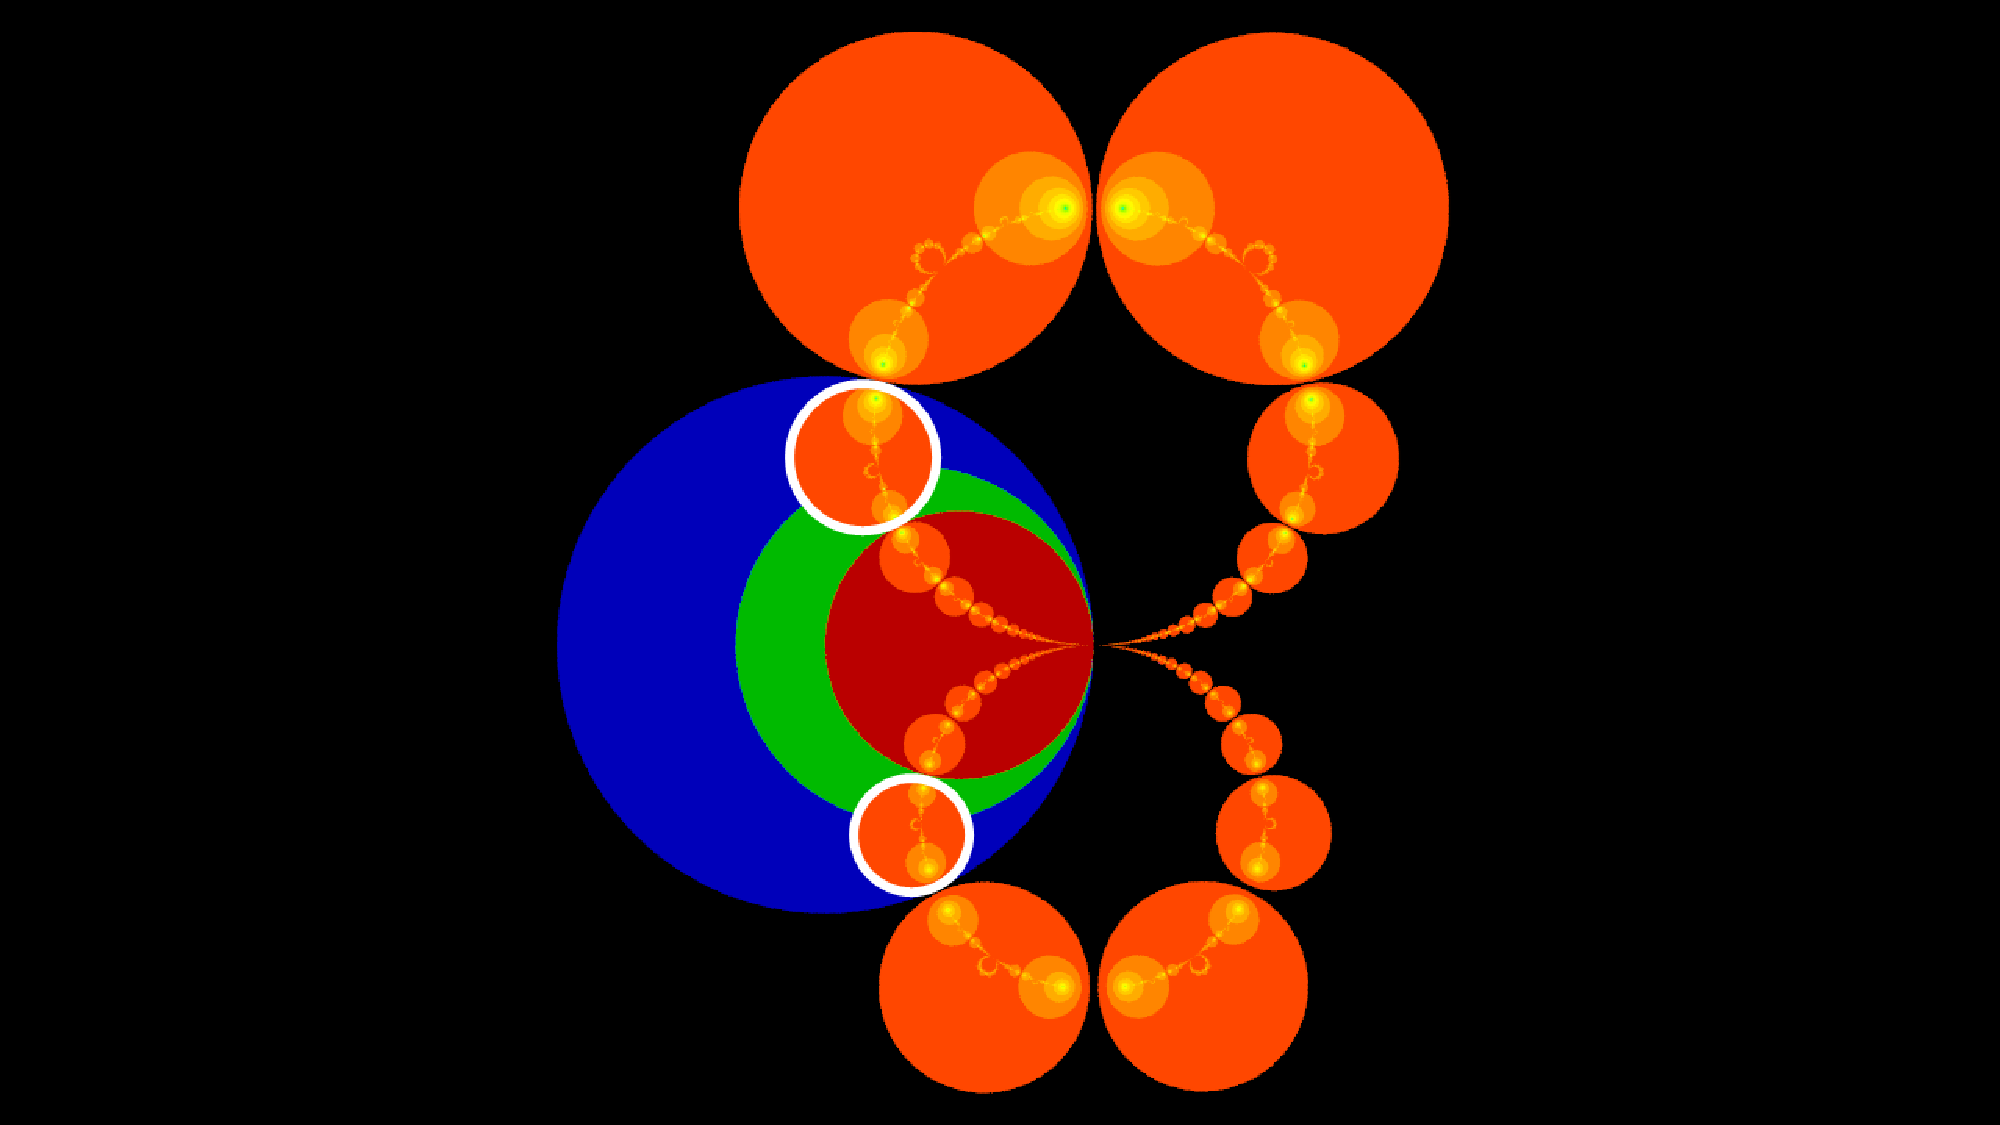
\includegraphics[width=2in, height=2in, keepaspectratio]{../img/klein/2diis/parabolic.pdf}
   \subcaption{Parabolic}
   \label{fig:parabolic2d}
  \end{minipage}
  \caption{Composition of two circles}
  \label{fig:twoCircles}
\end{figure}

\noindent\textbf{Loxodromic.}

上記の二つの円による反転の合成変換は実数による拡縮と共役であった.
この生成元にさらに二つの反転を加えることでその軌道に捻りを加えることができる.
図\ref{fig:loxodromic2d}における$C1$と$C2$の中心を通る白い直線を$L$,
黄色の円を$C3$,そして水色の点を$P$とよぶ.
$P$は制御点であり,この点に$C1$の反転を作用させて得られた点を$P'$,$C2$の
反転を作用させて得られた点を$P''$とする.
$C3$は$P,~P',~P''$の三点から定義される.
$L$と$C3$の反転の合成は双曲型変換の軌道に捻りを加える回転となる.
また,固定点は$L$と$C3$の交点である.

写像$G$は以下のようになる.
\begin{align*}
G =
\begin{cases}
 (I_{C2} \circ I_{C1}) \circ (I_{C3} \circ I_L) & (\text{The point is inside of } C1) \\
 (I_L \circ I_{C3}) \circ (I_{C1} \circ I_{C2}) & (\text{The point is outside of }C1')
\end{cases}
\end{align*}

また,二つの固定点からこの種類の生成元を得ることもできる.
このときの生成元を図\ref{fig:loxoFixed}に示した.
図においてふたつ赤色の点を固定点$FP1$,$FP2$とする.
ふたつの桃色の点を制御点$Q1$,$Q2$,水色の点を制御点$P$とする.
変換を構成する円と直線である$C1,~C2,~C3,~L$は以下のように求めることがで
きる.
\begin{align*}
 L &= line(FP1,~FP2)\\
 C3 &= circle(P,~FP1,~FP2)\\
 C1 &= circle(Q1,~I_{C3}(Q1),~I_{L}(Q1))\\
 C2 &= circle(Q2,~I_{C3}(Q2),~I_{L}(Q2))
\end{align*}

\begin{figure}[htbp]
 \begin{minipage}[t]{0.5\hsize}
  \center
   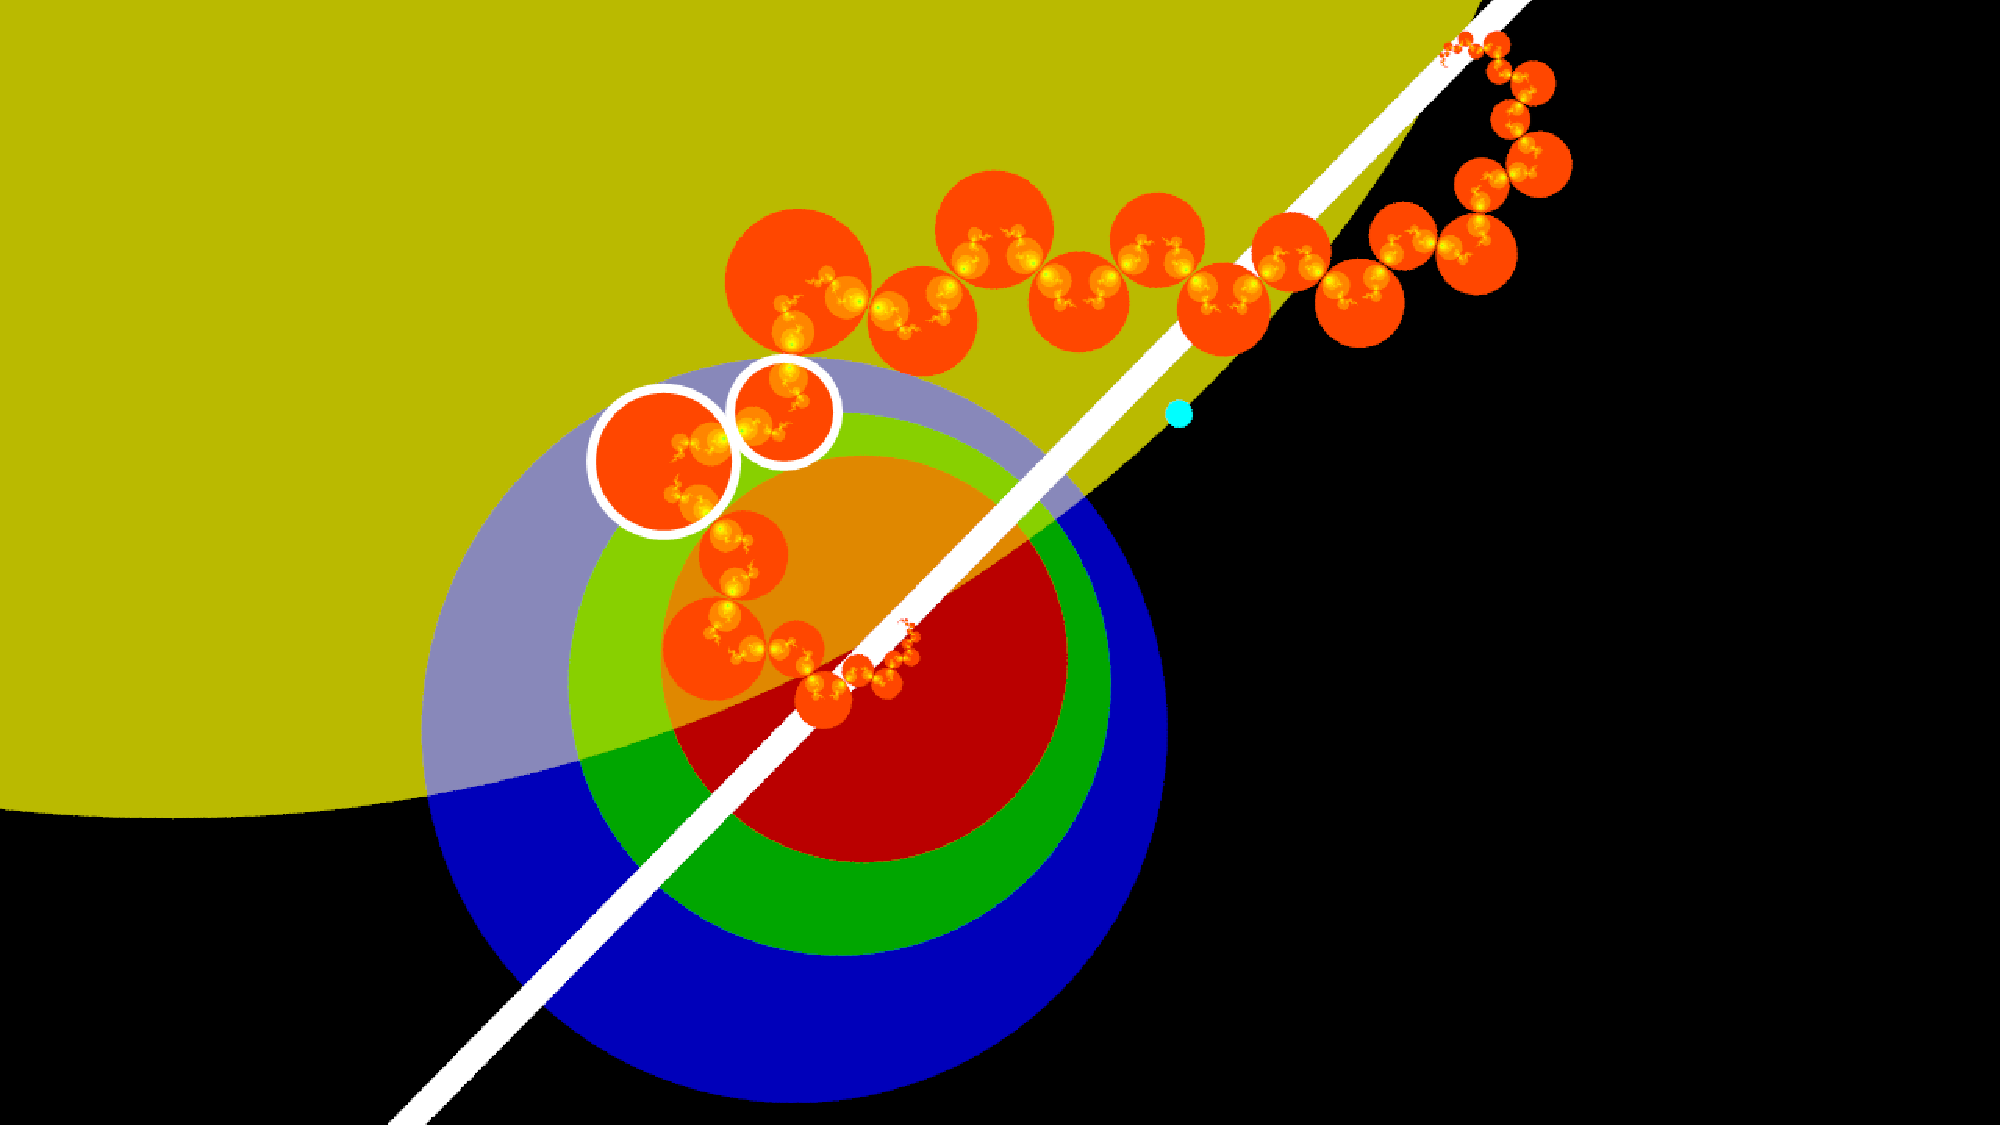
\includegraphics[width=2in, height=2in, keepaspectratio]{../img/klein/2diis/loxoEdged.pdf}
   \caption{Loxodromic transformation}
   \label{fig:loxodromic2d}
 \end{minipage}
 \begin{minipage}[t]{0.5\hsize}
  \center
  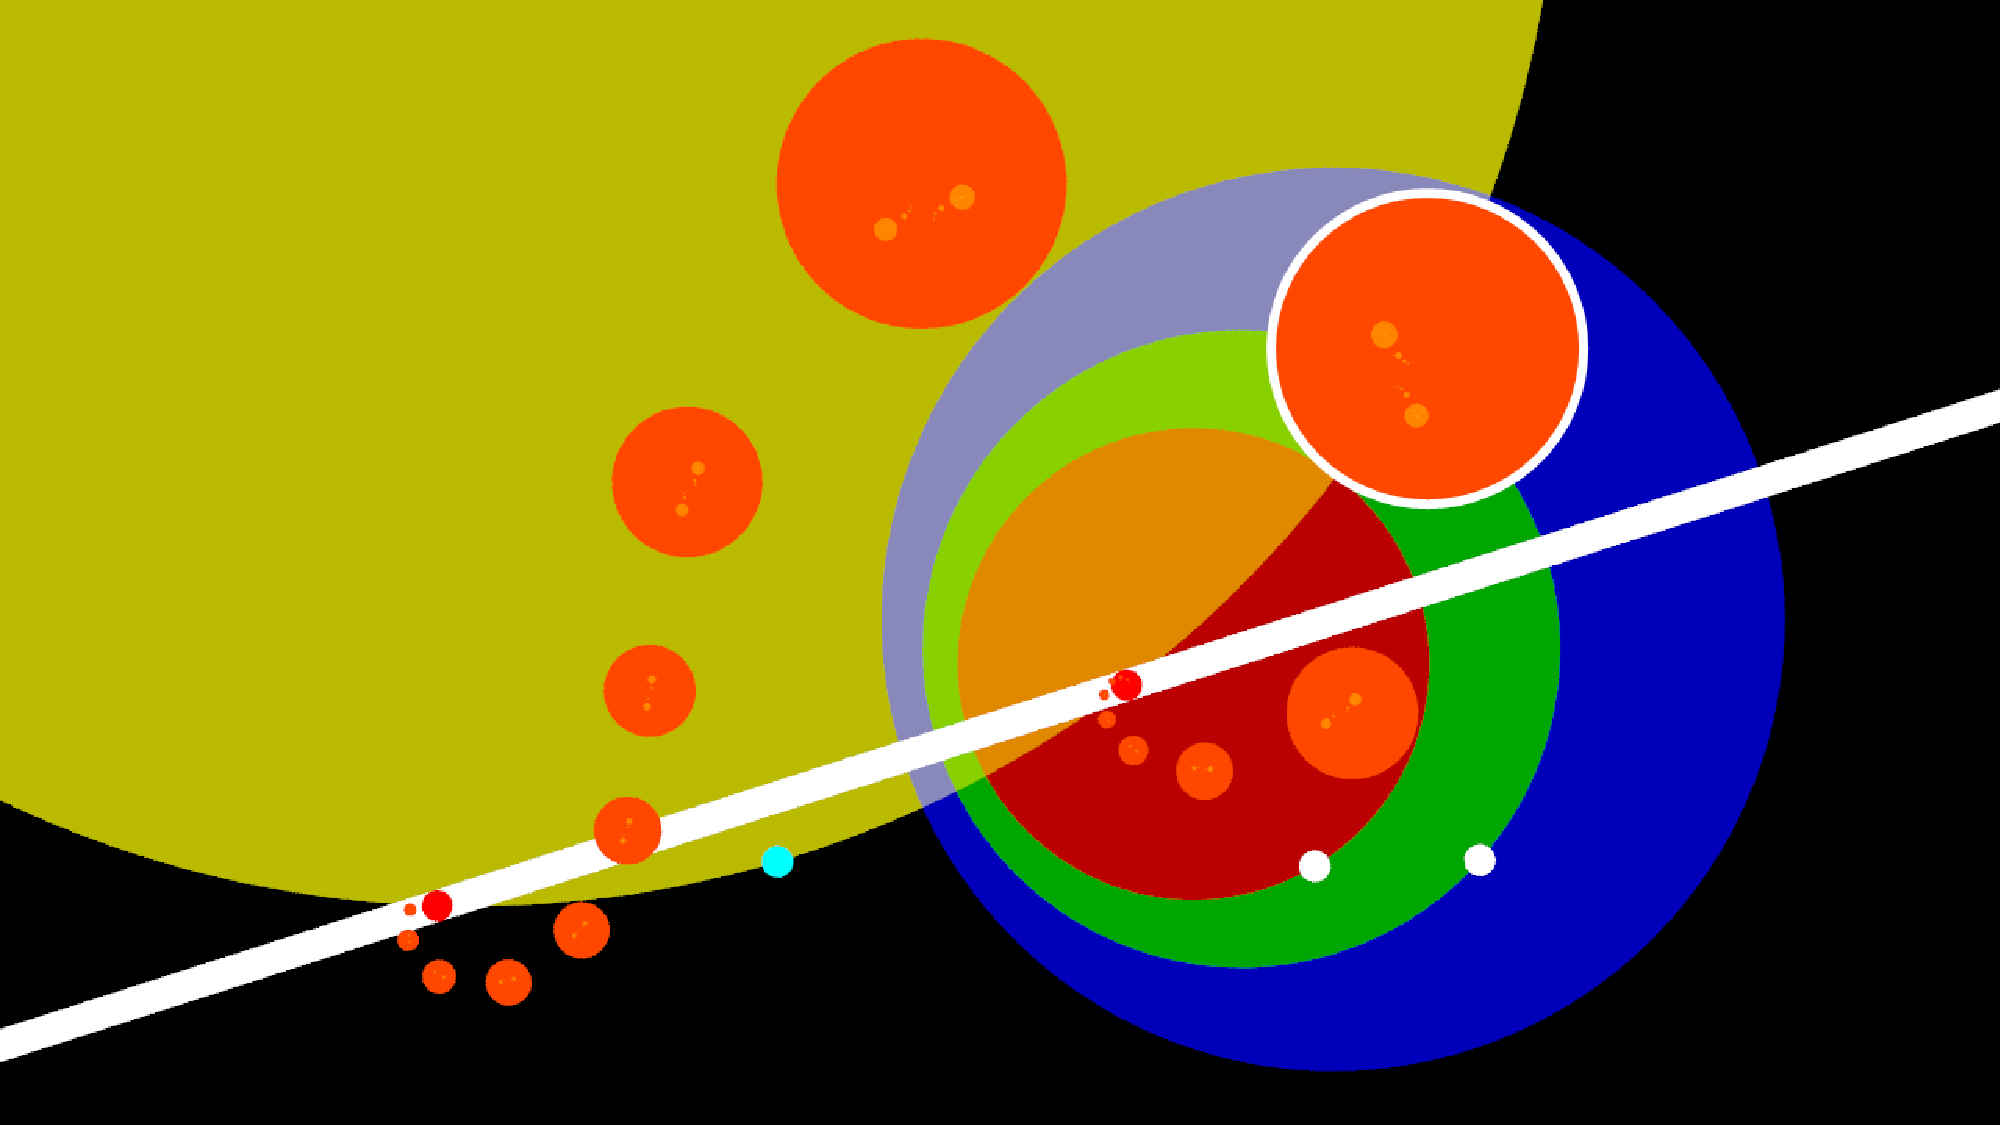
\includegraphics[width=2in, height=2in,
  keepaspectratio]{../img/klein/2diis/loxoFixedEdged.pdf}
  \caption{Loxodromic transformation defined by two fixed points}
  \label{fig:loxoFixed}
 \end{minipage}
\end{figure}

\subsubsection{3D Generators}

球に関する反転の合成で三次元空間に作用するメビウス変換を得る.
ほとんどの三次元の生成元は円を球に拡張することで自然に導くことが
できる.三次元の群は基本球を反転球による反転の組み合わせで移した軌道を
描画することで可視化する.

\noindent\textbf{Simple Inversion.}

二次元の場合と同様に球の反転単体はメビウス変換ではなく,二つの球のペアに
よる反転がメビウス変換である.

\noindent\textbf{Inversion of a Sphere with Infinite Radius.}

半径が無限大の球の面は平面とみることができるので,その反転は平面による反
転として表すことができる.
図\ref{fig:infSphereGen}では青い板が半径が無限の球を表現している.
図\ref{fig:infSphereOrb}における右側の球の軌道はこの板によって左側へと
移されているため,軌道の左右に対称性をみることができる.

\noindent\textbf{Rotation.}

二次元の場合と同様にして,互いに交わる二つの平面の反転によって
回転を表すことができる.
回転軸は二枚の平面の交線で,なす角の二倍が回転角となる.
図\ref{fig:rotation3d}では180度の回転を示した.

\noindent\textbf{Parallel Translation.}

図\ref{fig:translation3d}に示されるような二枚の平行な平面による反転の組
は平面の法線方向への平行移動を表わす.
これは無限遠点に固定点をもつ放物型変換である.
基本領域は二枚の平面の間になる.

\noindent\textbf{Compound Parabolic.}

更に,三次元では平行移動の軌道に捻りを加えることができる.
図\ref{fig:compParabolic}では軌道に平行移動が作用されるたびに回転
が加えられていることがわかる.
この生成元は\emph{複合放物型変換}(\textit{Compound Parabolic})とよばれ,
高次元特有のものである.

\begin{figure}[h!tbp]
 \begin{minipage}[]{0.49\hsize}
  \begin{minipage}[]{0.24\hsize}
   \center
   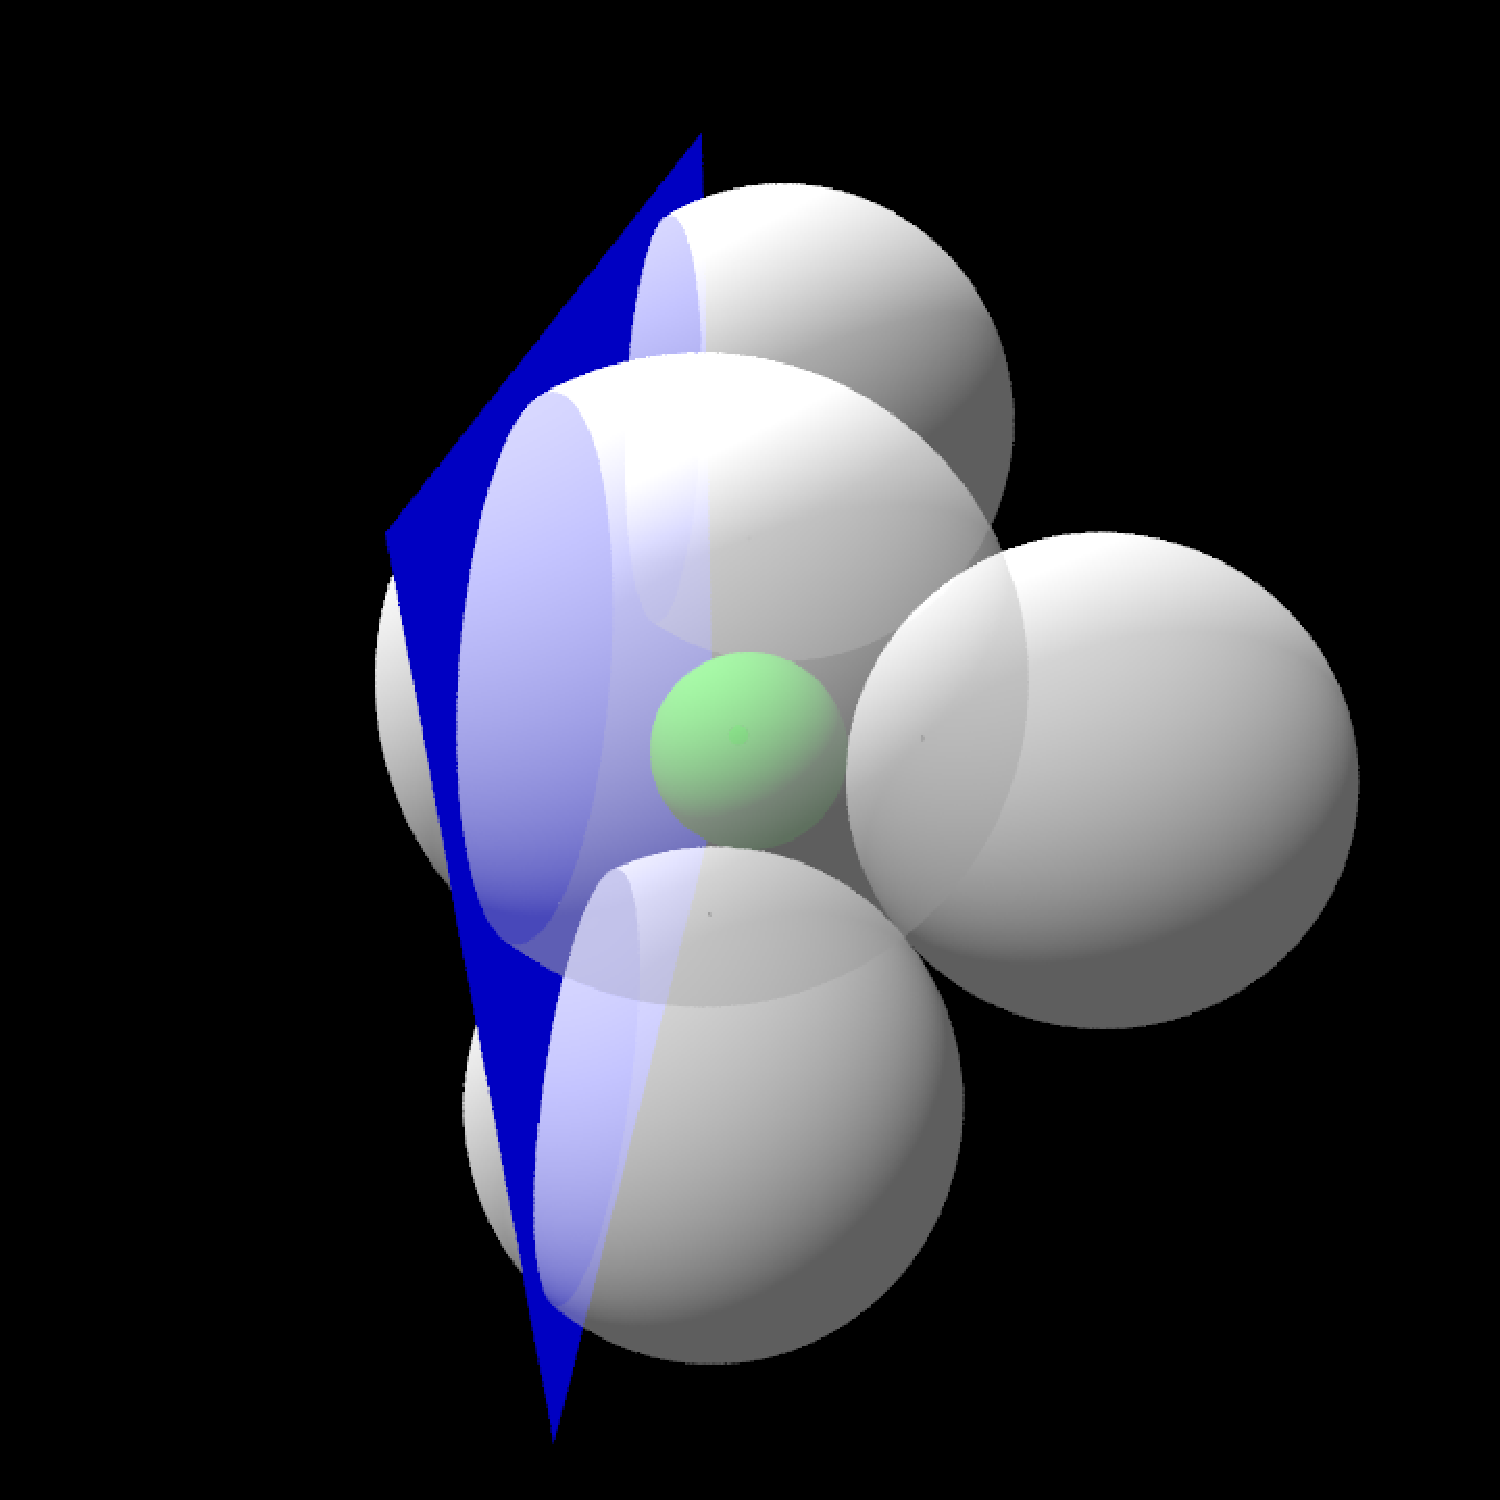
\includegraphics[width=1.5in, height=1.5in, keepaspectratio]{../img/klein/3diis/infSphereGen.pdf}
   \subcaption{Generator}
   \label{fig:infSphereGen}
  \end{minipage}
  \hspace*{\fill}
  \begin{minipage}[]{0.24\hsize}
   \center
   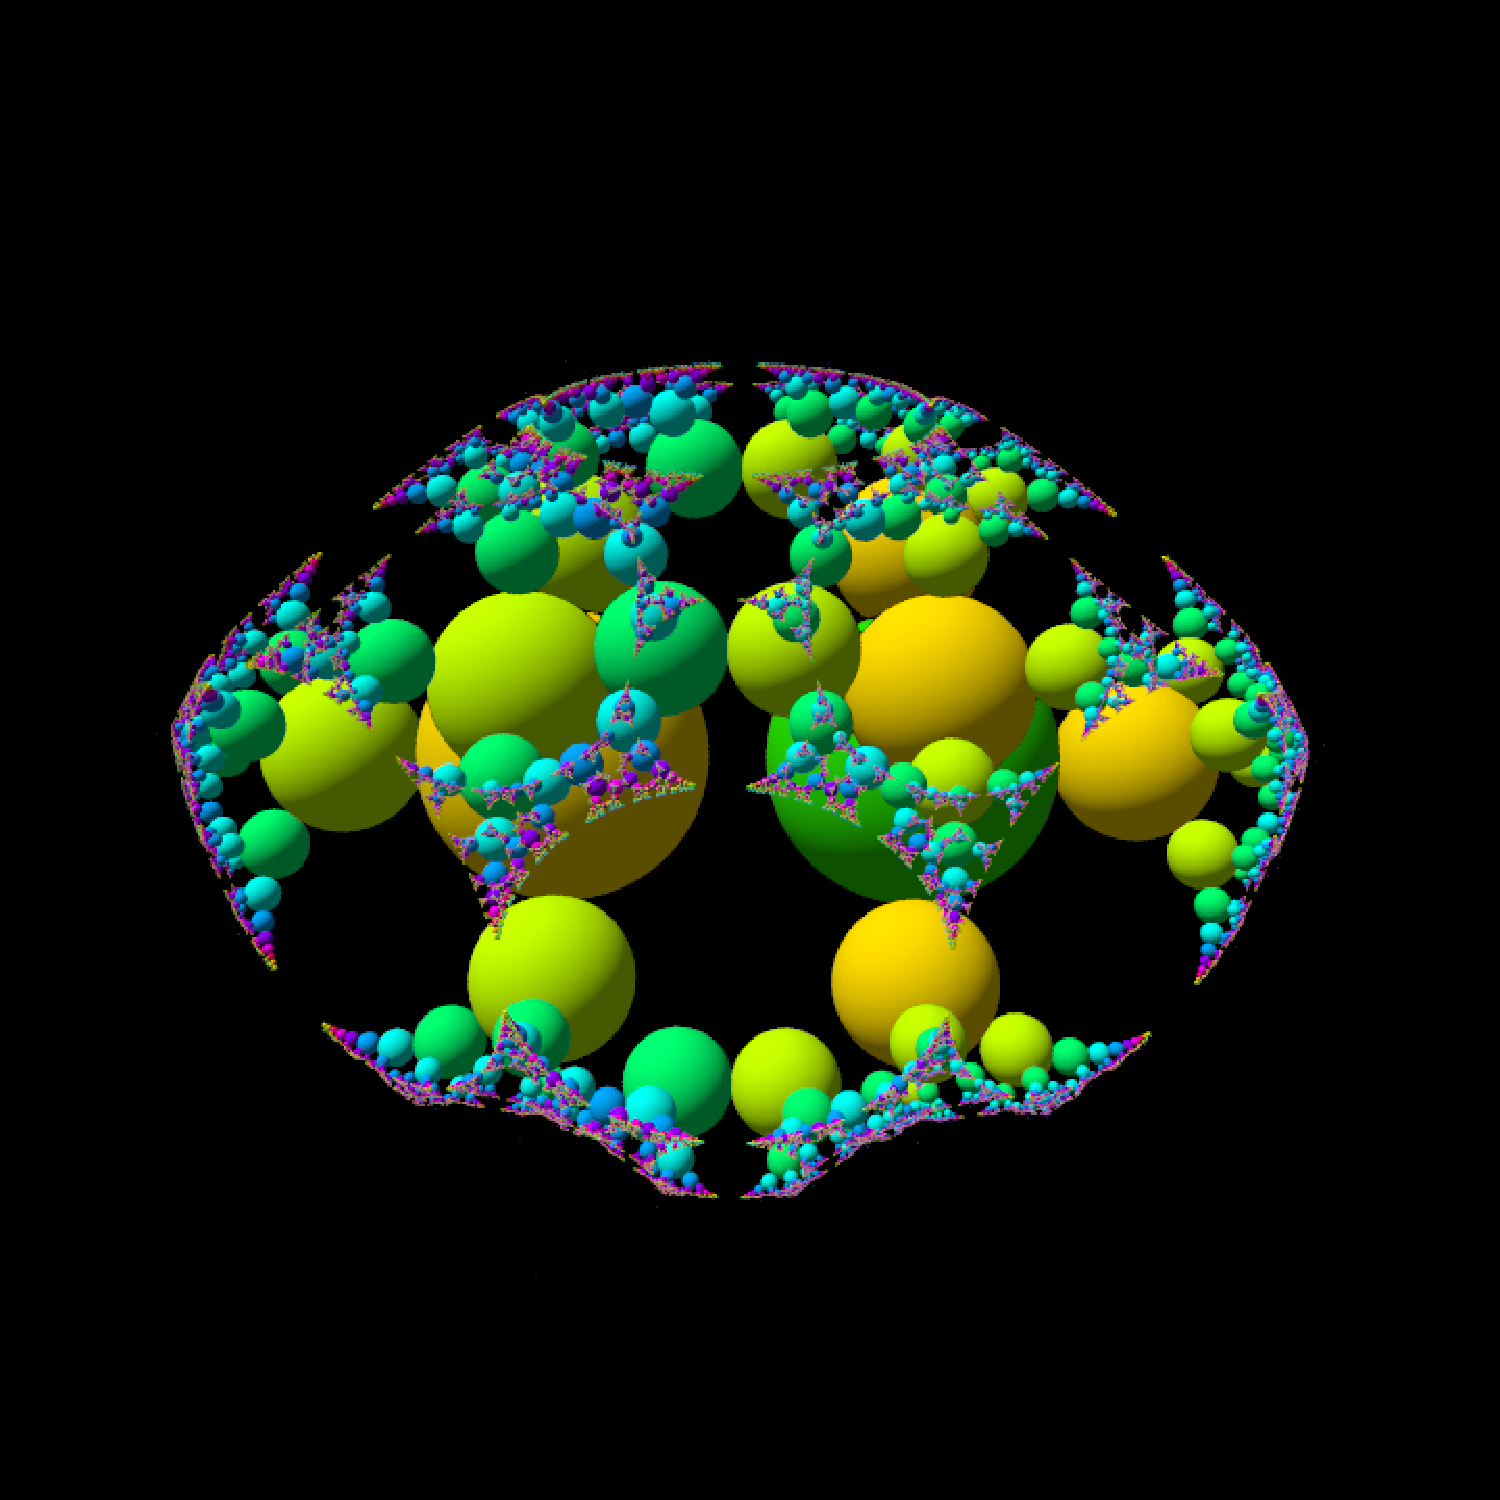
\includegraphics[width=1.5in, height=1.5in, keepaspectratio]{../img/klein/3diis/infSphereOrbit.pdf}
   \subcaption{Orbit}
   \label{fig:infSphereOrb}
  \end{minipage}
  \hspace*{\fill}
  \caption{Inversion of the Sphere with infinite radius}
  \label{fig:infSphere}
 \end{minipage}
 \begin{minipage}[]{0.49\hsize}
  \begin{minipage}[]{0.24\hsize}
   \center
   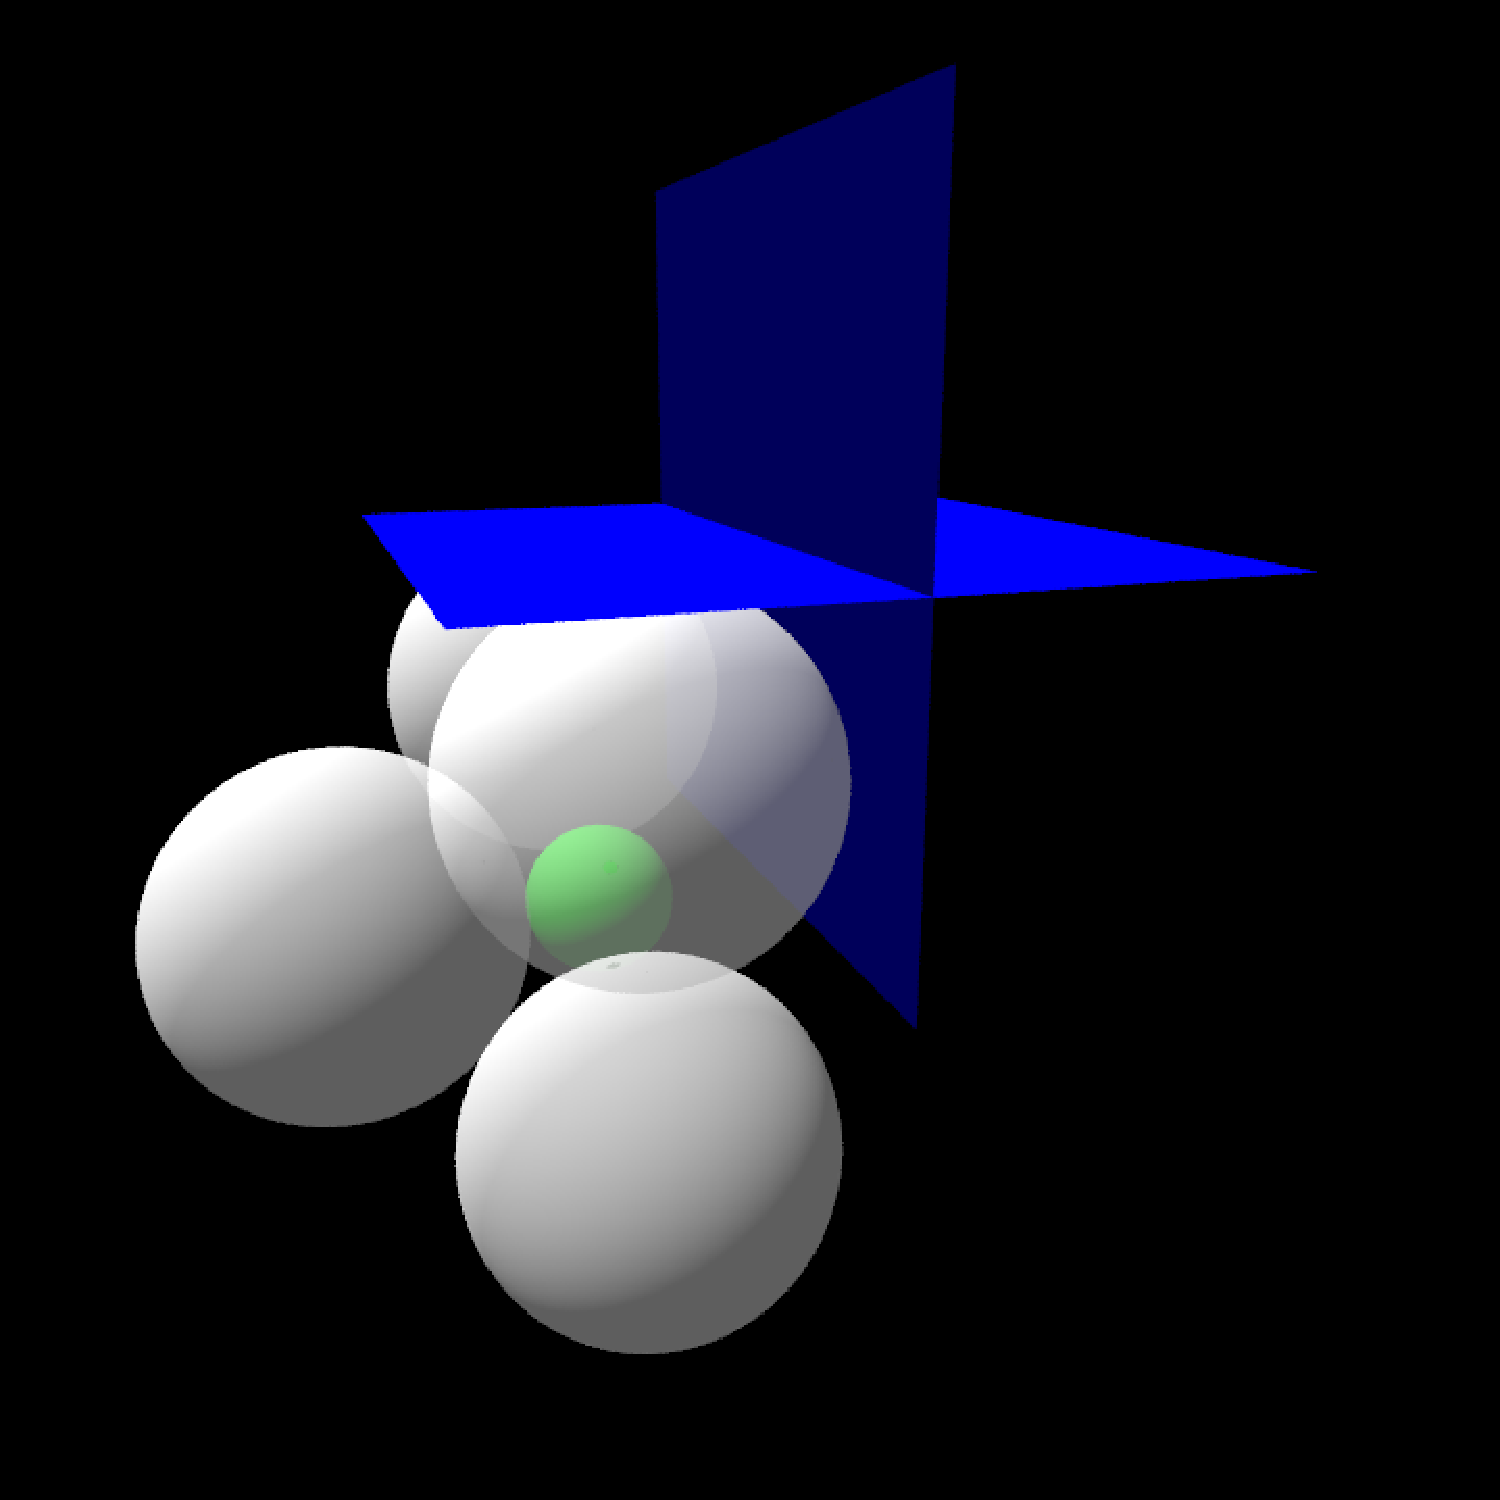
\includegraphics[width=1.5in, height=1.5in, keepaspectratio]{../img/klein/3diis/rotationGen.pdf}
   \subcaption{Generator}
   \label{fig:rotationGen}
  \end{minipage}
  \hspace*{\fill}
  \begin{minipage}[]{0.24\hsize}
   \center
   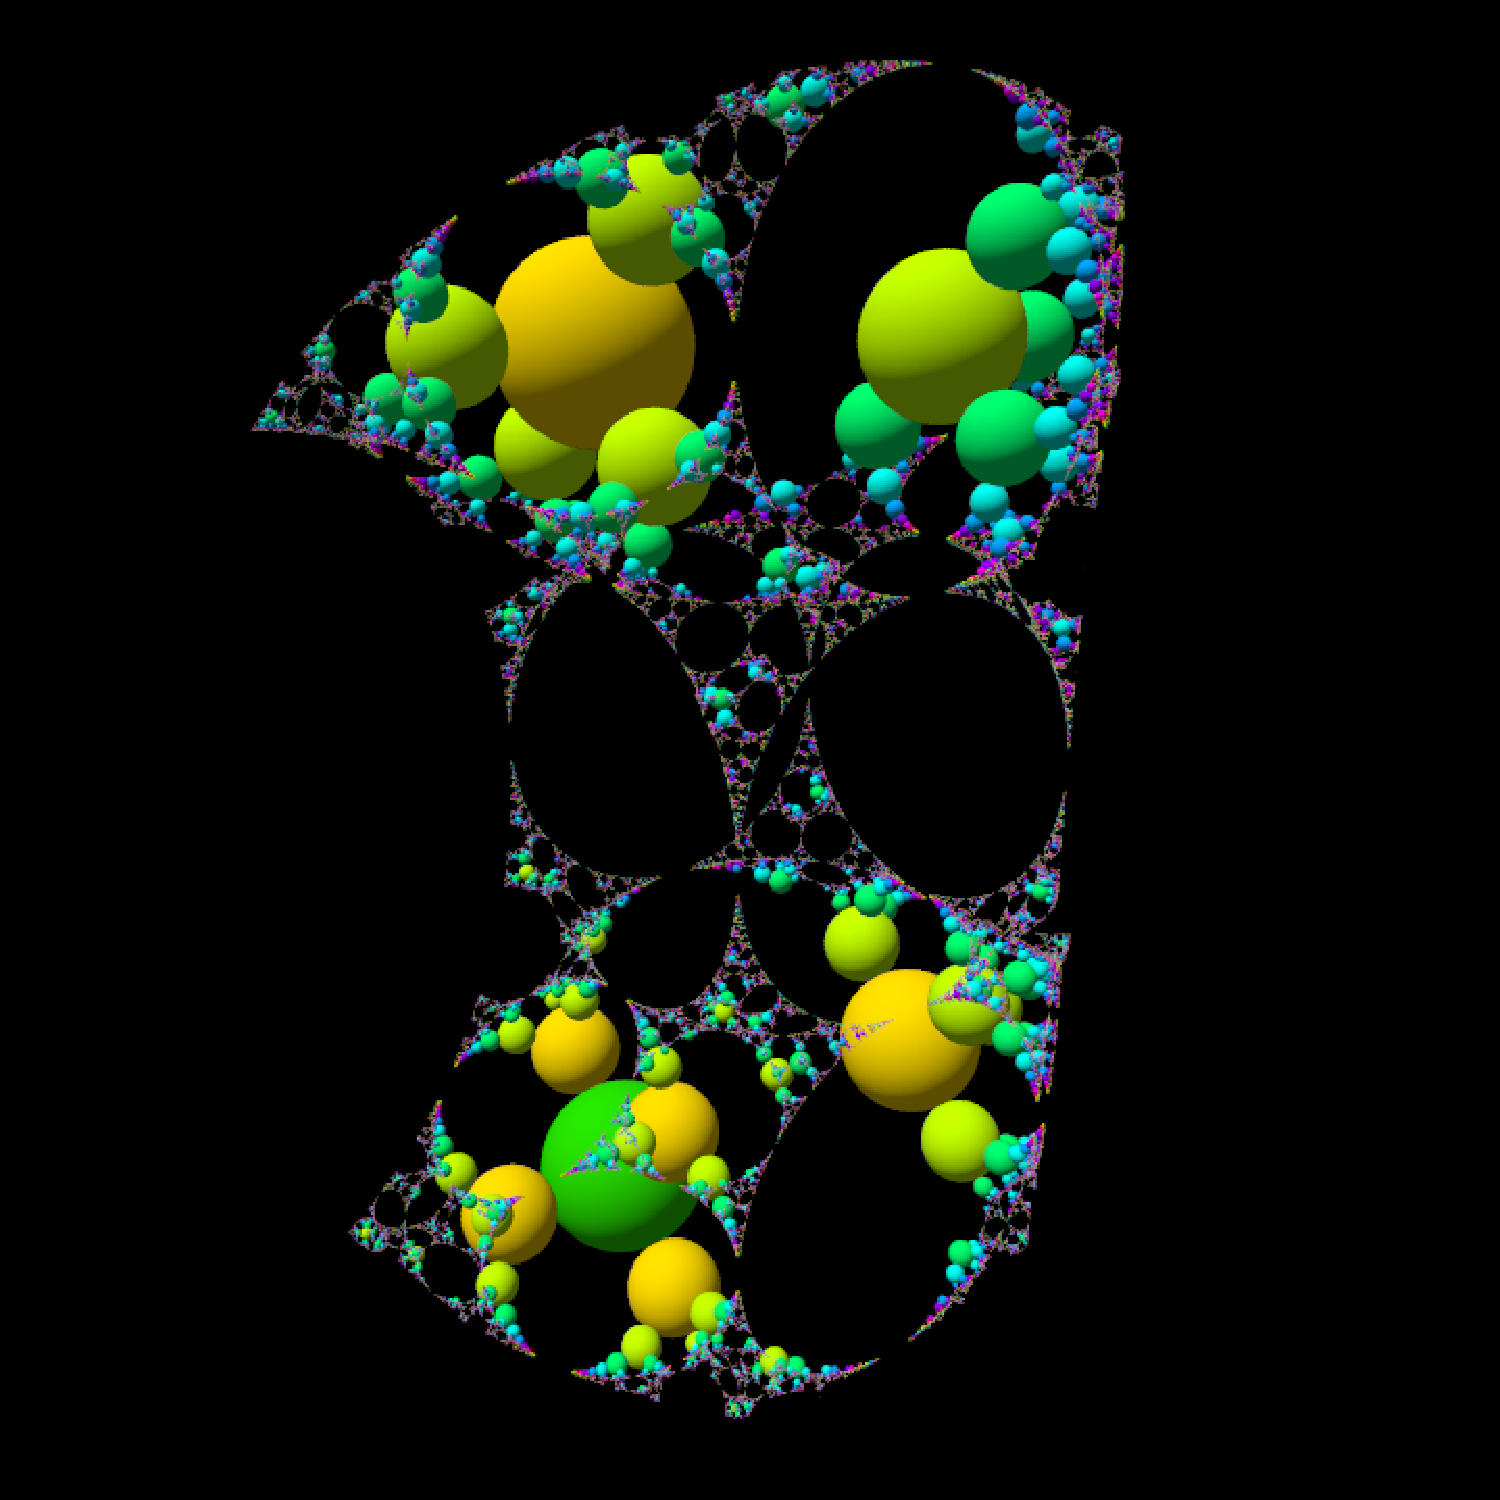
\includegraphics[width=1.5in, height=1.5in, keepaspectratio]{../img/klein/3diis/rotationOrb.pdf}
   \subcaption{Orbit}
   \label{fig:rotationOrb}
  \end{minipage}
  \hspace*{\fill}
  \caption{Rotation}
  \label{fig:rotation3d}
 \end{minipage}
\end{figure}

\begin{figure}[h!tbp]
 \begin{minipage}{0.49\hsize}
  \begin{minipage}{0.24\hsize}
   \center
   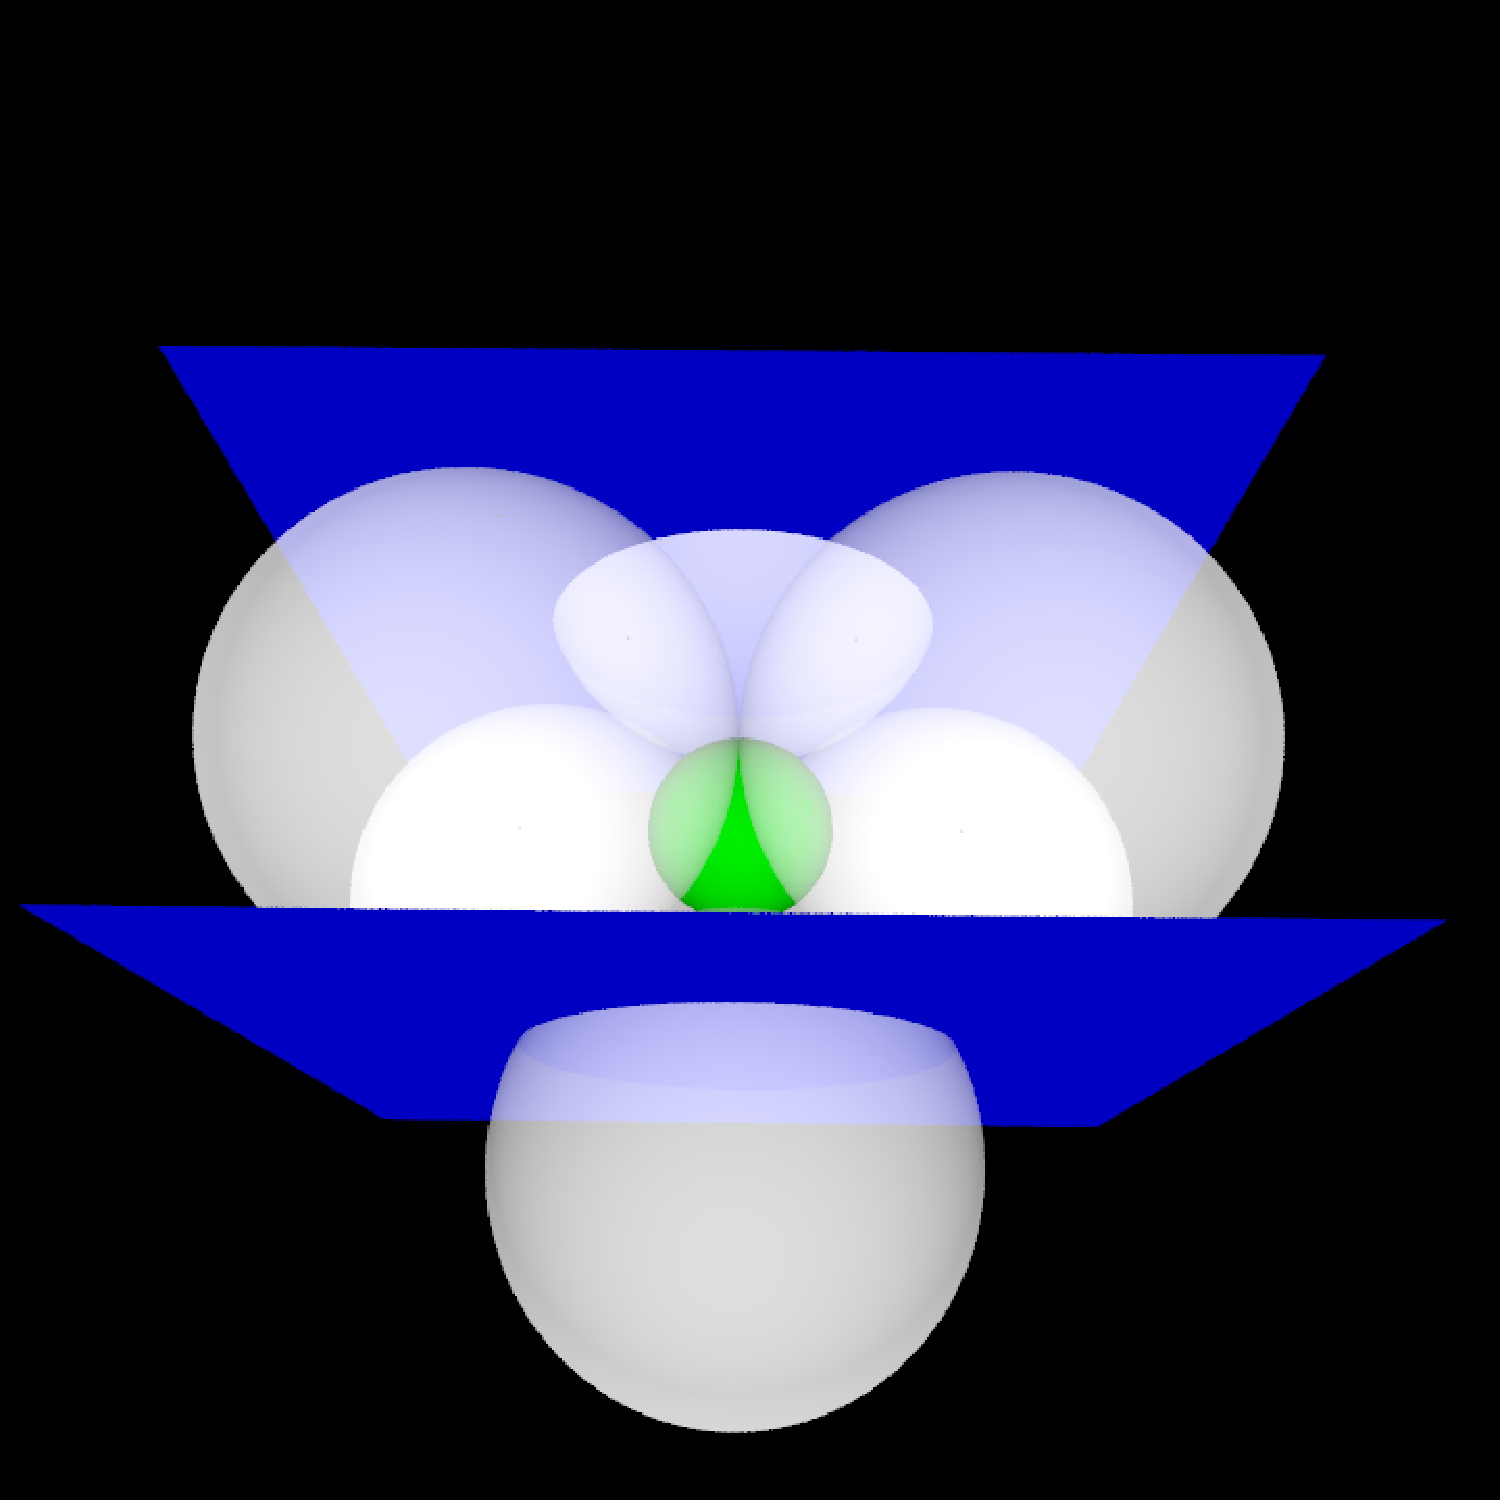
\includegraphics[width=1.5in, height=1.5in, keepaspectratio]{../img/klein/3diis/translationGen.pdf}
   \subcaption{Generator}
   \label{fig:translationGen}
  \end{minipage}
  \hspace*{\fill}
  \begin{minipage}{0.24\hsize}
   \center
   \includegraphics[width=1.5in, height=1.5in, keepaspectratio]{../img/klein/3diis/translationOrbit.pdf}
   \subcaption{Orbit}
   \label{fig:translationOrb}
  \end{minipage}
  \hspace*{\fill}
  \caption{Parallel translation}
  \label{fig:translation3d}
 \end{minipage}
 \begin{minipage}{0.49\hsize}
  \begin{minipage}{0.24\hsize}
   \center
   \includegraphics[width=1.5in, height=1.5in, keepaspectratio]{../img/klein/3diis/compParabolicGen.pdf}
   \subcaption{Generator}
   \label{fig:compParabolicGen}
  \end{minipage}
  \hspace*{\fill}
  \begin{minipage}{0.24\hsize}
   \center
   \includegraphics[width=1.5in, height=1.5in, keepaspectratio]{../img/klein/3diis/compParabolicOrb.pdf}
   \subcaption{Orbit}
   \label{fig:compParabolicOrb}
  \end{minipage}
  \hspace*{\fill}
  \caption{Compound parabolic transformation}
  \label{fig:compParabolic}
 \end{minipage}
\end{figure}

\noindent\textbf{Composition of Two Spheres}

二次元の場合と同様に二つの球の反転を組み合わせた生成元を定義することができる.
図\ref{fig:loxoGen3d}に示される赤い球を$S1$,黄緑の球を$S2$,
青い球を$S1'$とよぶとき,写像$G$は以下のようになる.
\begin{align*}
G =
\begin{cases}
 I_{S2} \circ I_{S1} & (\text{The point is inside of } S1) \\
 I_{S1} \circ I_{S2} & (\text{The point is outside of }S1')
\end{cases}
\end{align*}
$S1$と$S2$に接触がない場合,この生成元は斜航型変換となる.
軌道は図\ref{fig:loxoOrb3d}に示した.
この生成元に6つの反転球を加えた群の軌道が\ref{fig:loxoOrbSch3d}のようになる.

図\ref{fig:parabolicGen3d}のように,$S1$と$S2$が一点で接触するとき,この
生成元は放物型変換となる.
固定点は球同士の接点となり,軌道は図\ref{fig:parabolicOrb3d}のように一点
に収束する.

\noindent\textbf{Compound Loxodromic}

最後に,$S1$と$S2$に直交する二つの球を追加する.
図\ref{fig:compLoxoGen}に示される桃色の球を$S3$,黄色の球を$S4$,
3つの制御点を$P,Q1,Q2$とよぶ.
$P$に$S1$の反転を作用させて得られた点と,$S2$の
反転を作用させて得られた点をそれぞれ$P'$,$P''$とする.
そして,写像$G$は以下のようになる.
\begin{align*}
S3 &= sphere(P,~P',~P'',~Q1) \\
S4 &= sphere(P,~P',~P'',~Q2) \\
G &=
\begin{cases}
 (I_{S4} \circ I_{S3}) \circ (I_{S1} \circ I_{S2}) & (\text{The point is inside of } S1) \\
 (I_{S2} \circ I_{S1}) \circ (I_{S3} \circ I_{S4}) & (\text{The point is
 outside of } S1')\\
\end{cases}
\end{align*}
$S3$と$S4$の反転の合成は回転を表す.
この生成元の軌道を示した図\ref{fig:compLoxoOrb}では,二次元における斜航
型変換のような三次元空間における捻じれた軌道をみることができる.
この生成元は\emph{複合斜航型変換}(Compound Loxodromic)とよばれ,高次元特
有のメビウス変換である.

\begin{figure}[h!tbp]
 \begin{minipage}{0.24\hsize}
  \center
  \includegraphics[width=1.5in, height=1.5in, keepaspectratio]{../img/klein/3diis/loxoGenSimple.pdf}
  \subcaption{Generator}
  \label{fig:loxoGen3d}
 \end{minipage}
 \hspace*{\fill}
 \begin{minipage}{0.24\hsize}
  \center
   \includegraphics[width=1.5in, height=1.5in, keepaspectratio]{../img/klein/3diis/loxoOrbSimple.pdf}
   \subcaption{Orbit}
   \label{fig:loxoOrb3d}
 \end{minipage}
 \hspace*{\fill}
 \begin{minipage}{0.24\hsize}
  \center
  \includegraphics[width=1.5in, height=1.5in, keepaspectratio]{../img/klein/3diis/loxoSchottkyGen.pdf}
  \subcaption{Generator}
  \label{fig:loxoOrbSchGen3d}
 \end{minipage}
 \hspace*{\fill}
 \begin{minipage}{0.24\hsize}
  \center
  \includegraphics[width=1.5in, height=1.5in, keepaspectratio]{../img/klein/3diis/loxoOrbSch.pdf}
  \subcaption{Orbit}
  \label{fig:loxoOrbSch3d}
 \end{minipage}
 \caption{Loxodromic transformation}
 \label{fig:loxodromic3d}
\end{figure}

\begin{figure}[h!tbp]
  \begin{minipage}{0.24\hsize}
   \center
   \includegraphics[width=1.5in, height=1.5in, keepaspectratio]{../img/klein/3diis/parabolicOneGen.pdf}
   \subcaption{Generator}
   \label{fig:parabolicGen3d}
  \end{minipage}
  \hspace*{\fill}
  \begin{minipage}{0.24\hsize}
   \center
   \includegraphics[width=1.5in, height=1.5in, keepaspectratio]{../img/klein/3diis/parabolicOneOrb.pdf}
   \subcaption{Orbit}
   \label{fig:parabolicOrb3d}
  \end{minipage}
  \hspace*{\fill}
  \begin{minipage}{0.24\hsize}
   \center
   \includegraphics[width=1.5in, height=1.5in, keepaspectratio]{../img/klein/3diis/parabolicGen.pdf}
   \subcaption{Generator}
   \label{}
  \end{minipage}
 \hspace*{\fill}
 \begin{minipage}{0.24\hsize}
  \center
  \includegraphics[width=1.5in, height=1.5in, keepaspectratio]{../img/klein/3diis/parabolicOrb.pdf}
  \subcaption{Orbit}
   \label{}
 \end{minipage}
 \hspace*{\fill}
  \caption{Parabolic transformation}
 \label{}
\end{figure}

\begin{figure}[h!tbp]
  \begin{minipage}{0.24\hsize}
   \center
   \includegraphics[width=1.5in, height=1.5in, keepaspectratio]{../img/klein/3diis/compLoxoOneGen.pdf}
   \subcaption{Generator}
   \label{fig:compLoxoGen}
  \end{minipage}
 \hspace*{\fill}
 \begin{minipage}{0.24\hsize}
  \center
  \includegraphics[width=1.5in, height=1.5in, keepaspectratio]{../img/klein/3diis/compLoxoOneOrb.pdf}
  \subcaption{Orbit}
   \label{fig:compLoxoOrb}
 \end{minipage}
 \hspace*{\fill}
  \begin{minipage}{0.24\hsize}
   \center
   \includegraphics[width=1.5in, height=1.5in, keepaspectratio]{../img/klein/3diis/compLoxoGen.pdf}
   \subcaption{Generator}
   \label{}
  \end{minipage}
 \hspace*{\fill}
 \begin{minipage}{0.24\hsize}
  \center
  \includegraphics[width=1.5in, height=1.5in, keepaspectratio]{../img/klein/3diis/compLoxoOrb.pdf}
  \subcaption{Orbit}
   \label{}
 \end{minipage}
 \hspace*{\fill}
  \caption{Compound loxodromic transformation}
 \label{fig:compLoxo}
\end{figure}

\subsubsection{Optimization}

写像$G$を用いて点を基本領域へ移すためには$G$を繰り返し点に作用させる必要
がある.
しかし,いくつかの写像は適切な共役をとることによって点を一度の操作で基本
領域に移動させることができる.
このような最適化は特に固定点への収束が遅い放物型変換の軌道を描くこ
とに役立つ.
この節では二次元の生成元の最適化についてまとめる.
もちろん,三次元の生成元に関しても以下で述べる方法と同様のアプローチで最
適化することができる.

\noindent\textbf{Parallel Translation.}

まずは図\ref{fig:translation2d}と同様の平行な二直線の組による平行移動を
考える.
繰り返し二直線に関する反転を作用させる代わりに剰余を用いて点を移すこと
ができる.

まず始めに,平行移動と回転の合成によって
平行な二直線の一方をX軸に垂直に,もう一方の直線がY軸に沿うようにする共役
変換$T$を求める.
共役変換で移された生成元は図\ref{fig:translationMod}に示した.
写像に与えられた点$P$を$T$で移した点$T(P)$を基本領域上の点である$P'$に移
すことを考える.
$w$を二直線の距離,$i$を平行移動によって移された半径無限の円の指数,
$d$と$d'$をY軸からの距離とする.
$d$を$w$で割ることにより,剰余$d'$と商$i$を得ることができる.
$d'$を用いて$T(P)$から$P'$を計算し,これを$T^{-1}$で元の座標に戻す.
以上の操作を一度行うことで,平面上の全ての点を平行移動の生成元の基本領域
に移すことができる.
また,$i$から,通常の反転を何回行なうことで基本領域へと移すことができる
かを求めることができる.

\noindent\textbf{Parabolic.}

次に図\ref{fig:parabolic2d}のような放物型変換を考える.
まず共役変換$T$をこの放物型変換の固定点を中心とする円の反転とする.
$T$を$C1,~C2,~C1'$に対して適用すると,固定点は無限遠点に移るので,三本の平行な直
線を得ることができる.
それぞれの直線を$TC1,~TC2,~TC1'$とよぶ.
図\ref{fig:parabolicMod}にこれらの直線を示した.
赤の直線$TC1$と青の直線$TC1'$が平行移動を表す.

最適化された写像の操作過程は以下のようになる.
まず,写像に与えられた点${P}$に$T$を作用させた点$T(P)$を得る.
そして,$T(P)$を前述の平行移動と同様の操作で移し,点$P'$を得る.
最後にもう一度$T(= T^{-1})$を$P'$に作用させて元の座標に移すことで基本領
域上の点を得る.

\noindent\textbf{Loxodromic.}

最後に図\ref{fig:hyperbolic2d}のような双曲型変換を考える.
この変換の片方の固定点を中心にもつ円に関する反転を共役変換$T$とする.
そして,$T$を$C1,~C2,~C1'$に作用させて得られた円をそれぞれ
$TC1,~TC2,~TC1'$とよぶ.
これらは変換のもう一方の固定点に$T$を作用させた点を中心にもつ同心円となる.

これらの円を図\ref{fig:hyperbolicMod}に示した.
これまで同様に写像に与えられた点$P$を$T$で移した点$T(P)$を基本領域上の点
である$P'$に移すことを考える.
図において,$r$と$r'$を$TC1$と$TC1'$の半径,$d$を$T(P)$と同心円の中心か
らの距離,$d'$を$P'$と同心円の中心からの距離とする.
$k$を倍数,$q$を指数係数,$i$を円列の指数とする.
これらは以下のように計算される.
 \begin{align*}
  k& = \frac{r'}{r}\\
  q& = \log_{k} \frac{d}{r}\\
  d'& = r \cdot k^{fracionalPart(q)}\\
  i& = floor(q)
 \end{align*}
$d'$を用いて$T(P)$を基本領域へと移した点である$P'$を計算することが
できる.また,$i$から最適化前の変換を何度点に作用させると基本領域へと移
せるかがわかる.

ここで,考える変換が図\ref{fig:loxodromic2d}のような斜航型変換であるとき,
$T$を$L$と$C3$にも作用させることでこの変換も最適化することができる.
$T$によって得られた$L$と$C3$の像をそれぞれ$TL$と$TC3$とよぶ.
$L$と$C3$は二つの固定点を通るので,$TL$と$TC3$は同心円の中心で交わる二直
線となり,これらの反転の組み合わせが同心円の中心を回転中心とする回転を表
す.

$T$によって移された生成元を図\ref{fig:loxodromicMod}に示した.
白の直線が$TL$,黄色の直線が$TC3$である.
斜航型変換では$P'$を得た後で$P'$に回転を与えて$P''$を得る.
回転角を$\varphi$,$TL$と$TC3$のなす角を$\theta$と
すると,$\varphi$は$\varphi = 2 \theta i$で計算することができる.

上記の処理をまとめると以下のようになる.
まず,$T$を与えられた点$P$に適用し,$T(P)$を得る.
$TC1$,$TC1'$から$d'$を算出し,$P'$を計算する.
もしも$TL$,$TC3$があれば,同心円の中心を回転中心として$P'$を$\varphi$回転
させ,$P''$を得る.
最後にもう一度$T$を$P'$もしくは$P''$に作用させ,元の座標に戻すことで基本
領域上の点を得る.

\begin{figure}[h!tbp]
 \begin{minipage}[t]{0.24\hsize}
  \center
  \includegraphics[width=1.5in, height=1.5in, keepaspectratio]{../img/klein/2diis/translationModTP.pdf}
  \caption{Parallel translation}
  \label{fig:translationMod}
 \end{minipage}
 \hspace*{\fill}
 \begin{minipage}[t]{0.24\hsize}
  \center
  \includegraphics[width=1.5in, height=1.5in, keepaspectratio]{../img/klein/2diis/parabolicModTP.pdf}
  \caption{Inverted parabolic generator}
  \label{fig:parabolicMod}
 \end{minipage}
 \hspace*{\fill}
 \begin{minipage}[t]{0.24\hsize}
  \center
  \includegraphics[width=1.5in, height=1.5in, keepaspectratio]{../img/klein/2diis/hyperbolicMod.pdf}
  \caption{Inverted hyperbolic generator}
  \label{fig:hyperbolicMod}
 \end{minipage}
 \hspace*{\fill}
 \begin{minipage}[t]{0.24\hsize}
  \center
  \includegraphics[width=1.5in, height=1.5in, keepaspectratio]{../img/klein/2diis/loxodromicModRotation.pdf}
  \caption{Inverted loxodromic generator}
  \label{fig:loxodromicMod}
  \hspace*{\fill}
 \end{minipage}
\end{figure}

\subsection{Other Topics}

ここまでは『インドラの真珠』における話題と筆者による成果をまとめた.
この節ではクライン群の研究の中でも興味深い図像を見ることができる先行研
究とその他の可視化手法を簡単に紹介する.

\subsubsection{Quasi Fuchsian 3D Fractals}

阿原・荒木は擬フックス群を三次元に拡張した4次元クライン群を考案した
\cite{ahara2003sphairahedral}\cite{ahara2003sphaira}.
これはQuasi Fuchsian 3D Fractalsとよばれ,
フラクタルコミュニティに大きな影響を与えたといわれている.

図\ref{fig:schottky}において,中央の円盤に囲まれた基本領域を\emph{円辺形}と
よぶ.
擬フックス群は円辺形を囲む円の組から生成元を得ることができる.
そこで円辺形を三次元に拡張した\emph{球面体}(\textit{Sphairahedron})を定義
することで三次元の擬フックス群を構成することができる.

図\ref{fig:sphairahedron}には6つの球に囲まれた球面体を示した.
この球面体をそれを囲む球の反転で移していくことで極限集合を得ることができ
る.図\ref{fig:quasiFuchsian}にその極限集合を示した.
円辺形による擬フックス群の極限集合は円の和集合となる.したがって,球面体
による擬フックス群の極限集合は球の和集合となる.

阿原・荒木による動画\footnote{Quasi-fuchsian fractals:
\url{https://www.youtube.com/watch?v=3lcO9zRCv-4}}ではこのフラクタルの構
成過程をみることができる.

また,レイマーチングとDistance Estimationによる高速描画のアルゴリズムが
2012年にKnightyによって開発された
\footnote{Another 3D Kleinian:
 \url{http://www.fractalforums.com/ifs-iterated-function-systems/another-3d-kleinian/}}
 .
図\ref{fig:quasi-fuchsian-3d}はKnightyによるFragmentariumのスクリプトを用
いてレンダリングした.


荒木はこのフラクタル図形の物質化についてまとめている
\cite{araki2006materializing}.
円辺形や球面体の数学的な事項については蔭山
がまとめている\cite{kageyama2016masterSphaira}.


\begin{figure}[htbp]
 \begin{minipage}{0.49\hsize}
  \center
  \includegraphics[width=3in, height=3in, keepaspectratio]{../img/klein/sphairahedron1.pdf}
  \subcaption{}
 \end{minipage}
 \hspace*{\fill}
 \begin{minipage}{0.49\hsize}
  \center
  \includegraphics[width=3in, height=3in, keepaspectratio]{../img/klein/sphairahedron2.pdf}
  \subcaption{}
 \end{minipage}
 \caption{Sphairahedron}
 \label{fig:sphairahedron}
\end{figure}

\begin{figure}[htbp]
 \begin{minipage}{0.49\hsize}
  \center
  \includegraphics[width=2.5in, height=2.5in, keepaspectratio]{../img/klein/quasi-fuchsian.pdf}
  \subcaption{}
 \end{minipage}
 \hspace*{\fill}
 \begin{minipage}{0.49\hsize}
  \center
  \includegraphics[width=2.5in, height=2.5in, keepaspectratio]{../img/klein/quasi-fuchsian2.pdf}
  \subcaption{}
 \end{minipage}
 \caption{Quasi Fuchsian}
 \label{fig:quasiFuchsian}
\end{figure}

\subsubsection{Other 4D Kleinian Groups}

『インドラの真珠』でみるクライン群は複素平面に作用するメビウス変換から構成されている.
現在,このようなクライン群はほぼ研究され尽されてしまった.
しかし,高次元のクライン群はまだわかっていないことが多い.
先に述べたように三次元空間に作用するメビウス変換は四元数を用い
て定義することができる.
これは$Sp^k(1,~1)$とよばれ,2x2の四元数行列で表現される.
四元数で構成されるメビウス変換とその分類は佐久川による
\cite{sakugawa2007master}や\cite{sakugawa2009accidental}にまとまっている.
これらの論文において,佐久川は複合放物型変換を含む群のレシピを考案
している.
図\ref{fig:sakugawa}はそのレシピで生成された群の極限集合を描画したものである.

\begin{figure}[h!tbp]
 \begin{minipage}{0.49\hsize}
  \center
  \includegraphics[width=3in, height=3in, keepaspectratio]{../img/klein/sakugawa1.pdf}
  \subcaption{}
 \end{minipage}
 \hspace*{\fill}
 \begin{minipage}{0.49\hsize}
  \center
  \includegraphics[width=3in, height=3in, keepaspectratio]{../img/klein/sakugawa2.pdf}
  \subcaption{}
 \end{minipage}
 \begin{minipage}{0.49\hsize}
  \center
  \includegraphics[width=3in, height=3in, keepaspectratio]{../img/klein/sakugawa3.pdf}
  \subcaption{}
 \end{minipage}
 \hspace*{\fill}
 \begin{minipage}{0.49\hsize}
  \center
  \includegraphics[width=3in, height=3in, keepaspectratio]{../img/klein/sakugawa4.pdf}
  \subcaption{}
 \end{minipage}
 \caption{The limit set of the 4D Kleinian Groups}
 \label{fig:sakugawa}
\end{figure}

また,荒木・糸はマスキット群を高次元に拡張することで四次元クライン群のレ
シピを考案した\cite{araki2008extension}
\footnote{4-dimensional Kleinian punctured torus groups:
\url{http://www.math.nagoya-u.ac.jp/~itoken/3d-maskit/3d-maskit.html}}.
この論文中では幾何学的性質をうまく使うことで,四元数の計算を避けている.
佐久川はこの群の四元数表示を導出した\cite{sakugawa2010limit}.

三浦は3つ以上の生成元による4次元クライン群をモジュラー群から構成するこ
とを試みた\cite{miura2015master}.
筆者はこの論文における数値実験と可視化を行った.

\subsubsection{Once Punctured Torus Groups}

クライン群の部分群である一点穴開きトーラス群({\it Once Punctured Torus Groups})は
和田による{\it OPTi}\footnote{OPTi:
\url{http://delta-mat.ist.osaka-u.ac.jp/OPTi/index.html}}という描画ソフ
トウェアによって大きく研究が進んだ.
描画や離散性判定のためのアルゴリズムが開発者の和田によりまとめられている
\cite{wada2003optiDrawingLimit}\cite{wada2006optiDiscreteness}.
この群の極限集合は図\ref{fig:opt}のようになる.

 \begin{figure}[htbp]
  \begin{minipage}{0.5\hsize}
   \center
   \includegraphics[width=3in, height=3in,
   keepaspectratio]{../img/klein/opt1N.pdf}
   \subcaption{}
  \end{minipage}
  \begin{minipage}{0.5\hsize}
   \center
   \includegraphics[width=3in, height=3in,
   keepaspectratio]{../img/klein/opt2N.pdf}
   \subcaption{}
  \end{minipage}
  \caption{The Limit Set of the once punctured torus groups}
  \label{fig:opt}
 \end{figure}

\subsubsection{Other Rendering Approach}

ここまでに述べたクライン群の可視化手法とは別のアルゴリズムも存在する.

Aaron MontagはIterated Inversion Systemを用いて極限集合を描画する方法を
提案した\cite{Montag2014hyperbolicIFS}
\footnote{Kleinian Groups WebGL:
 \url{https://www-m10.ma.tum.de/bin/view/Lehrstuhl/AaronMontagKleinian}}.
これはテクスチャベースで実装されており,GPUで高速に描画される.

また,Jos Ley,Knightyはマスキット群におけるEscape-timeアルゴリズムの式
とDistance Estimationを考案した
\footnote{An escape time algorithm for Kleinian group limit set:\\ \quad
\quad
\url{http://www.fractalforums.com/3d-fractal-generation/an-escape-tim-algorithm-for-kleinian-group-limit-sets/}}
.
このアルゴリズムは二次元だけでなく,三次元の極限集合の描画にも対応している.
荒木・糸\cite{araki2008extension}が考えた群と同様に,一方に平行移動を含
む2つの放物型変換による群を考えている.
詳細なアルゴリズムに関してはJos Leyがまとめている
\footnote{Mathematical Imagery, An escape-time algorithm for a family of
Kleinian groups:\\ \quad \quad \url{http://www.josleys.com/article_show.php?id=221}}.

\subsection{Further Readings}

この章の最後に,クライン群の数学的な背景を学習するための書籍をいくつか挙げておく.
クライン群論は双曲幾何学という分野に属している.
双曲幾何学の入門書には『双曲幾何学への招待』
\cite{taniguchi_okumura199610invitation}や
『双曲幾何』\cite{mitani200409hyperbolicGeometry}がある.
クライン群の数学的内容に踏み込んだ書籍には『双曲多様体とクライン群』
\cite{taniguchi_matsuzaki_hyperbolicManifold}や『Outer Circles』
\cite{Marden200705outerCircles}がある.
また,レクチャーノート集に『Kleinian Group and Hyperbolic 3-Manifolds』
\cite{Y._V._C.200311}や
『Spaces of Kleinian Groups』\cite{Yair_Makoto_Caroline200606}がある.

\clearpage